%%%%%%%%%%%%%%%%%%%%%%%%%%%%%%%%%%%%%%%%%
% Thesis 
% LaTeX Template
% Version 1.3 (21/12/12)
%
% This template has been downloaded from:
% http://www.latextemplates.com
%
% Original authors:
% Steven Gunn 
% http://users.ecs.soton.ac.uk/srg/softwaretools/document/templates/
% and
% Sunil Patel
% http://www.sunilpatel.co.uk/thesis-template/
%
% License:
% CC BY-NC-SA 3.0 (http://creativecommons.org/licenses/by-nc-sa/3.0/)
%
% Note:
% Make sure to edit document variables in the Thesis.cls file
%
%%%%%%%%%%%%%%%%%%%%%%%%%%%%%%%%%%%%%%%%%

%----------------------------------------------------------------------------------------
%	PACKAGES AND OTHER DOCUMENT CONFIGURATIONS
%----------------------------------------------------------------------------------------

\documentclass[11pt, a4paper, oneside]{Thesis} % Paper size, default font size and one-sided paper

\makeatletter								
\newcommand{\vo}[1]{\vec{#1}\@ifnextchar{^}{\,}{}} %function to draw vectors such that the arrow doesn't overlap with the next superscipt
\makeatother


\def\be{\begin{equation}}

\def\ee{\end{equation}}


\graphicspath{{./Pictures/}} % Specifies the directory where pictures are stored

\usepackage[square, numbers, comma, sort&compress]{natbib} % Use the natbib reference package - read up on this to edit the reference style; if you want text (e.g. Smith et al., 2012) for the in-text references (instead of numbers), remove 'numbers' 
\usepackage{color}
\usepackage{verbatim}
\usepackage{graphicx}

\hypersetup{urlcolor=blue, colorlinks=true} % Colors hyperlinks in blue - change to black if annoying
\title{\ttitle} % Defines the thesis title - don't touch this

\begin{document}

\frontmatter % Use roman page numbering style (i, ii, iii, iv...) for the pre-content pages

\setstretch{1.3} % Line spacing of 1.3

% Define the page headers using the FancyHdr package and set up for one-sided printing
\fancyhead{} % Clears all page headers and footers
\rhead{\thepage} % Sets the right side header to show the page number
\lhead{} % Clears the left side page header

\pagestyle{fancy} % Finally, use the "fancy" page style to implement the FancyHdr headers

\newcommand{\HRule}{\rule{\linewidth}{0.5mm}} % New command to make the lines in the title page

% PDF meta-data
\hypersetup{pdftitle=\ttitle}
\hypersetup{pdfsubject=\subjectname}
\hypersetup{pdfauthor=\authornames}
\hypersetup{pdfkeywords=\keywordnames}

%----------------------------------------------------------------------------------------
%	TITLE PAGE
%----------------------------------------------------------------------------------------

\begin{titlepage}
\begin{center}

\textsc{\LARGE \univname}\\[1.5cm] % University name
\textsc{\Large \ttitle}\\[0.5cm] % Thesis type

\HRule \\[0.4cm] % Horizontal line
{\huge \bfseries \ttitle}\\[0.4cm] % Thesis title
\HRule \\[1.5cm] % Horizontal line
 
\begin{minipage}{0.4\textwidth}
\begin{flushleft} \large
\emph{Author:}\\
\href{http://www.johnsmith.com}{\authornames} % Author name - remove the \href bracket to remove the link
\end{flushleft}
\end{minipage}
\begin{minipage}{0.4\textwidth}
\begin{flushright} \large
\emph{Supervisor:} \\
\href{http://www.jamessmith.com}{\supname} % Supervisor name - remove the \href bracket to remove the link  
\end{flushright}
\end{minipage}\\[3cm]
 
\large \textit{A Minor Dissertation submitted in partial fulfilment of the requirements\\ for the degree of \degreename}\\[0.3cm] % University requirement text
\textit{in the}\\[0.4cm]
\groupname\\\deptname\\[2cm] % Research group name and department name
 
{\large \today}\\[4cm] % Date
%\includegraphics{Logo} % University/department logo - uncomment to place it
 
\vfill
\end{center}

\end{titlepage}

%----------------------------------------------------------------------------------------
%	DECLARATION PAGE
%	Your institution may give you a different text to place here
%----------------------------------------------------------------------------------------

\Declaration{

\addtocontents{toc}{\vspace{1em}} % Add a gap in the Contents, for aesthetics

I, \authornames, declare that this thesis titled, '\ttitle' and the work presented in it are my own. I confirm that:
\begin{itemize} 
\item[\tiny{$\blacksquare$}] This work was done wholly or mainly while in candidature for a research degree at this University.
\item[\tiny{$\blacksquare$}] Where any part of this thesis has previously been submitted for a degree or any other qualification at this University or any other institution, this has been clearly stated.
\item[\tiny{$\blacksquare$}] Where I have consulted the published work of others, this is always clearly attributed.
\item[\tiny{$\blacksquare$}] Where I have quoted from the work of others, the source is always given. With the exception of such quotations, this thesis is entirely my own work.
\item[\tiny{$\blacksquare$}] I have acknowledged all main sources of help.
\item[\tiny{$\blacksquare$}] Where the thesis is based on work done by myself jointly with others, I have made clear exactly what was done by others and what I have contributed myself.\\
\end{itemize}
 
Signed:\\
\rule[1em]{25em}{0.5pt} % This prints a line for the signature
 
Date:\\
\rule[1em]{25em}{0.5pt} % This prints a line to write the date
}

\clearpage % Start a new page

%----------------------------------------------------------------------------------------
%	QUOTATION PAGE
%----------------------------------------------------------------------------------------

\pagestyle{empty} % No headers or footers for the following pages

\null\vfill % Add some space to move the quote down the page a bit

\textit{``Thanks to my solid academic training, today I can write hundreds of words on virtually any topic without possessing a shred of information, which is how I got a good job in journalism."}

\begin{flushright}
Dave Barry
\end{flushright}

\vfill\vfill\vfill\vfill\vfill\vfill\null % Add some space at the bottom to position the quote just right

\clearpage % Start a new page

%----------------------------------------------------------------------------------------
%	ABSTRACT PAGE
%----------------------------------------------------------------------------------------

\addtotoc{Abstract} % Add the "Abstract" page entry to the Contents

\abstract{\addtocontents{toc}{\vspace{1em}} % Add a gap in the Contents, for aesthetics

The Thesis Abstract is written here (and usually kept to just this page). The page is kept centered vertically so can expand into the blank space above the title too\ldots
}
Hints as to what to include in your abstract:
Aim and objectives: What are the main themes, ideas or areas of theory being investigated?
Boundaries: What is the context and background to this dissertation? 
In what areas of theory or business practice should the reader concentrate their attention?
Methodology: What was/were the main method(s) employed to generate the results?
Results: What were your main findings?
Conclusions: What are the main conclusions that you arrive at when viewing the entire dissertation?
Recommendations: (if appropriate) What solutions do you offer in answer to the problems posed in the research objectives? 
\clearpage % Start a new page

%----------------------------------------------------------------------------------------
%	ACKNOWLEDGEMENTS
%----------------------------------------------------------------------------------------

\setstretch{1.3} % Reset the line-spacing to 1.3 for body text (if it has changed)

\acknowledgements{\addtocontents{toc}{\vspace{1em}} % Add a gap in the Contents, for aesthetics
No man is an island; nor is this thesis.
None of this would have happened if not for being introduced to machine learning by my supervisor Prof. Bruce Bassett.
Thank you for welcoming me in to the AIMS Cosmology group.
Your knowledge, patience and advice were invaluable when wading into unknown territory.
To Dr. Arun Kumar, thank you for always being willing to help with all the technical details, your advice and casual discussions helped me retain what sanity I have remaining.
To Kai Staats, thank you for bouncing around ideas with me, the office humour and surfing lessons.
To Lise du Buisson, this thesis builds on all the work you did in your MSc.Thesis.
Thank you for providing me with the grand tour of the data and all your research.
To the team at the SKA, in particular Laura Richter and Nadeem Ozeer, thank you for the warm welcome to the SKA world and access to computing resources.
Without your help my models would still be training.
To my girlfriend Francesca Favero thank you for checking every single word and concept and pushing me to complete this thesis.
Without you this thesis would never have left my laptop.
Last but not least, I am always indebted to my family and friends for their support.
}


\clearpage % Start a new page

%----------------------------------------------------------------------------------------
%	LIST OF CONTENTS/FIGURES/TABLES PAGES
%----------------------------------------------------------------------------------------

\pagestyle{fancy} % The page style headers have been "empty" all this time, now use the "fancy" headers as defined before to bring them back

\lhead{\emph{Contents}} % Set the left side page header to "Contents"
\tableofcontents % Write out the Table of Contents

\lhead{\emph{List of Figures}} % Set the left side page header to "List of Figures"
\listoffigures % Write out the List of Figures

\lhead{\emph{List of Tables}} % Set the left side page header to "List of Tables"
\listoftables % Write out the List of Tables

%----------------------------------------------------------------------------------------
%	ABBREVIATIONS
%----------------------------------------------------------------------------------------

\clearpage % Start a new page

\setstretch{1.5} % Set the line spacing to 1.5, this makes the following tables easier to read

\lhead{\emph{Abbreviations}} % Set the left side page header to "Abbreviations"
\listofsymbols{ll} % Include a list of Abbreviations (a table of two columns)
{
%\textbf{LAH} & \textbf{L}ist \textbf{A}bbreviations \textbf{H}ere \\

\textbf{AGN}  	& \textbf{A}ctive \textbf{G}alactic \textbf{N}uclei \\
\textbf{AI} 	& \textbf{A}rtificial \textbf{I}ntelligence \\
\textbf{ANN} 	& \textbf{A}rtificial \textbf{N}eural \textbf{N}etwork \\
\textbf{AUC} 	& \textbf{A}rea \textbf{U}nder \textbf{C}urve \\
\textbf{CNN} 	& \textbf{C}onvolutional \textbf{N}eural \textbf{N}etwork \\
\textbf{DL} 	& \textbf{D}eep \textbf{L}earning \\
\textbf{DNN} 	& \textbf{D}eep \textbf{N}eural \textbf{N}etwork\\
\textbf{FN} 	& \textbf{F}alse \textbf{N}egatives \\
\textbf{FP} 	& \textbf{F}alse \textbf{P}ositive \\
\textbf{FPR} 	& \textbf{F}alse \textbf{P}ositive \textbf{R}ate \\
\textbf{GPU} 	& \textbf{G}raphics \textbf{P}rocessing \textbf{U}nit \\
\textbf{LDSS} 	& \textbf{L}ow \textbf{D}ispersion \textbf{S}urvey \textbf{S}pectrograph \\
\textbf{LSST} 	& \textbf{L}arge \textbf{S}ynoptic \textbf{S}urvey \textbf{T}elescope \\
\textbf{ML} 	& \textbf{M}achine \textbf{L}earning \\
\textbf{MLP} 	& \textbf{M}ulti-\textbf{L}ayer \textbf{P}erceptron \\
\textbf{MSE} 	& \textbf{M}ean-\textbf{S}quared \textbf{E}rror \\
\textbf{RMS} 	& \textbf{R}oot \textbf{M}ean \textbf{S}quared \\
\textbf{ROC} 	& \textbf{R}eciever \textbf{O}perating \textbf{C}haracteristic \\
\textbf{SDSS} 	& \textbf{S}loan \textbf{D}igital \textbf{S}ky \textbf{S}urvey \\
\textbf{SGD} 	& \textbf{S}tochastic \textbf{G}radient \textbf{D}escent \\
\textbf{SN} 	& \textbf{S}uper\textbf{n}ova \\
\textbf{SNe} 	& \textbf{S}uper\textbf{n}ova\textbf{e} \\
\textbf{TN} 	& \textbf{T}rue \textbf{N}egatives \\
\textbf{TP} 	& \textbf{T}rue \textbf{P}ositives \\
\textbf{TPR} 	& \textbf{T}rue \textbf{P}ositive \textbf{R}ate \\

%\textbf{Acronym} & \textbf{W}hat (it) \textbf{S}tands \textbf{F}or \\
}

%----------------------------------------------------------------------------------------
%	PHYSICAL CONSTANTS/OTHER DEFINITIONS
%----------------------------------------------------------------------------------------

\clearpage % Start a new page

\lhead{\emph{Physical Constants}} % Set the left side page header to "Physical Constants"

\listofconstants{lrcl} % Include a list of Physical Constants (a four column table)
{
Speed of Light & $c$ & $=$ & $2.997\ 924\ 58\times10^{8}\ \mbox{ms}^{-\mbox{s}}$ (exact)\\
% Constant Name & Symbol & = & Constant Value (with units) \\
}

%----------------------------------------------------------------------------------------
%	SYMBOLS
%----------------------------------------------------------------------------------------

\clearpage % Start a new page

\lhead{\emph{Symbols}} % Set the left side page header to "Symbols"

\listofnomenclature{lll} % Include a list of Symbols (a three column table)
{
$a$ & distance & m \\
$P$ & power & W (Js$^{-1}$) \\
% Symbol & Name & Unit \\

& & \\ % Gap to separate the Roman symbols from the Greek

$\omega$ & angular frequency & rads$^{-1}$ \\
% Symbol & Name & Unit \\
}

%----------------------------------------------------------------------------------------
%	DEDICATION
%----------------------------------------------------------------------------------------

\setstretch{1.3} % Return the line spacing back to 1.3

\pagestyle{empty} % Page style needs to be empty for this page

\dedicatory{For/Dedicated to/To my\ldots} % Dedication text

\addtocontents{toc}{\vspace{2em}} % Add a gap in the Contents, for aesthetics

%----------------------------------------------------------------------------------------
%	THESIS CONTENT - CHAPTERS
%----------------------------------------------------------------------------------------

\mainmatter % Begin numeric (1,2,3...) page numbering

\pagestyle{fancy} % Return the page headers back to the "fancy" style

% Include the chapters of the thesis as separate files from the Chapters folder
% Uncomment the lines as you write the chapters

% Chapter 1

\chapter{Introduction} % Main chapter title

\label{1_Introduction} % For referencing the chapter elsewhere, use \ref{Chapter1} 

\lhead{\emph{Introduction}} % This is for the header on each page - perhaps a shortened title

%----------------------------------------------------------------------------------------
\begin{comment}
The Introduction to the dissertation should set out the background to the research study and address the following areas:
The context in which the research took place
- What is the background, the context, in which the research took place?
- Why is this subject or issue important
- Who are the key participants and/or ‘actors’ in the area under investigation?
- Are there important trends or pivotal variables of which the reader needs to be made aware?

- A clear and succinct statement of the aims and objectives that the dissertation is going to address.
- Have you presented a clear and unambiguous exposition of your research aim, the objectives you will address to meet this aim and your research questions?

The reasons why this study was carried out
- Was this study undertaken for example in order to test some aspect of professional or business practice or theory or framework of analysis?
- Was the research carried out to fulfil the demands of a business organisation?


This chapter may be between 500 to 750 words although in some subjects or topics the justification of the subject and scope may change the length of this chapter.


Introduction – brief overview explaining the background and importance of the study

3. Statement of Problem – specifically what the researcher wants to know; 

4. Purpose of the Study – explanation of the problem and what the researcher hopes to achieve by conducting the study

5. Theoretical framework, research questions, or objectives – used to guide the direction of the research;
\end{comment}
%Supernovae

%CONTEXT - Astronomy
Future astronomical surveys will generate far too much data for astronomers to tackle as they have traditionally done.
It was the norm for astronomers to eyeball images of the sky, looking for interesting objects or transients.
\textit{Transients} are objects that appear for a short amount of time.
These include, but are not limited to, asteroids, gamma ray bursts, supernovae or objects unknown to science altogether.
Telescopic cameras used in surveys have limited exposure to areas within the night sky,due to its vastness.
When transients are discovered, follow ups with other telescopes necessary in order to accurately identify the object.
Not all transients are created equal; some, like supernovae, are more valuable to science than others.
Supernovae are rare gems for cosmologists which allow for learning about the history, curvature and content of the Universe.

Telescope technology has improved so much transients are discovered at an overwhelming rate.
Astronomers lack the resources to follow up on every one.

The amount of data will be so large that the mere storage of it becomes a technological challenge, never mind computational use of it.
In addition, there is increased interest in studies that use data from telescopes sensitive to different wavelengths.
Such \textit{multi-wavelength} astronomy exacerbates the problem of handling and computing large amounts of data.
To appreciate the extent of the problem, consider the upcoming Large Synoptic Survey Telescope (LSST) which will become scientifically active in 2022\citep{abell2009lsst}.
Over its ten year lifespan it is estimated to discover over 10 billion galaxies.
Each day around 30 TB of raw image data will be generated that will require processing and reduction\citep{kantor2005lsst}.

The final archive will be around 60 PB, with the final object catalogue approximately 10-20 PB\citep{borne2007machine}.
This challenge calls for a new approach to astronomy, one that is capable of dealing with Big Data.
\textit{Big Data} is a broad term for data sets so large that traditional data processing methods are inadequate.
This is a problem that is now facing many fields and industries.
Maintaining the status quo will be impossible; other tools must be explored.
%pivotal variable end opf moors law, serial becoming parallel


%CONTEXT - Machine Learning
As data challenges have been building, the computer science world has had a renewed interest in Machine Learning.
\textit{Machine Learning} (ML) is the capacity of a computer program to `learn' from data.
For example, many pictures of a person can be shown to an algorithm such that it learns how to identify him/her in another photo without the explicit instruction of a programmer.
The reinvigorated interest in Machine Learning has largely been the result of an exponential growth in computing power.
Newly discovered training methods are impractical to implement on older computers.
Recently Machine Learning has shown great success in artificial intelligence and Big Data applications,  from the popularly used cellphone assistant Siri\citep{Siri} to driver-less Google cars\citep{waldrop2015no}.
Convolutional Neural Networks (CNNs), a machine learning method loosely inspired by the brain, have achieved near-human level performance at image recognition in as little time as a third of a second\citep{taigman2014deepface}.
This task, easy for us, has evaded the capability of computers and computer programmers for decades.
CNNs are an example of \textit{Deep Learning} (DL) algorithms.
They are `deep' in the sense that they use a many-layered architecture for learning.
Deep Learning has had incredible success in other domains too, from voice recognition, brain-machine interfaces and medical diagnoses illustrating its promise for many applications.


%PROBLEM STATEMENT
%AIM and Research objectives
While Machine Learning has had plenty of application in many arenas, it is still fairly new to astronomy.
The aim of this study is to establish whether or not Machine Learning has a positive role to play for the future of astronomy.
To answer this problem there are several research objectives to lead us to our aim.
First we must come to understand Machine Learning fundamentals.
In particular, we must learn what Deep Learning is and how to successfully apply it.
Second, we will need to identify a problem we can use as test-case of DL's effectiveness in astronomy.
For this we will apply DL to transient classification of the Sloan Digital Sky Survey (SDSS) from a few years ago, to observe the accuracy and efficiency achieved on a real-world astronomy dataset.
As CNNs have proven successful at image-recognition, they are the ML method of choice for this application.
This will act as a useful playground for exploring the role machine learning has for the future of astronomy.
The final research objective is the evaluation of ML's future in astronomy.

%Research Questions
The primary interest is to ascertain the extent to which ML is effective. 
To be a viable solution, machine learning must be both accurate and efficient.
Classification accuracy needs to be competitive with trained astronomers.

As supernovae are quite rare, about once in a hundred years per galaxy, ML must also be very stringent as to what constitutes a supernova.
If not, then the pool of objects classified as supernovae will be contaminated with countless false-positives and imaging artefacts.
This will waste resources on unnecessary and expensive follow-ups.
The ML algorithm must be able to operate in real-time with a large data influx in order to be efficient.
DL promises to outperform more classical ML approaches\citep{du2014machine}.
We will investigate the validity of this claim.
From our application we will see what DL can tell us about the SDSS transient data.

%Thesis Structure
This thesis has been structured in the following way:
Chapter 1 will use Neural Nets as a drawing board for understanding the inner workings of machine learning methods and their successful application.
We will need to know the subtleties of what is involved in machine learning and know how to evaluate our results in an objective way.
Chapter 2 will layout the nature of the test case.
We will detail what the SDSS sky survey entails; what data is collected and how it is structured. 
Next, the current status of ML transient classification will be investigated.
It is useful to see what others have discovered in their research.
Chapter 3 lays out the research methodology.
This will tackle the question of how to best achieve the research objectives in a logically sound way.
Chapter 4 will provide an analysis and discussion of the results.
Finally we conclude with closing remarks and future recommendations.



% Chapter 1

\chapter{Literature Review} % Main chapter title

\label{Chapter1} % For referencing the chapter elsewhere, use \ref{Chapter1} 

\lhead{Chapter 1. \emph{Literature Review}} % This is for the header on each page - perhaps a shortened title

%----------------------------------------------------------------------------------------
\begin{comment}

Review of the Literature – sufficient review of the relevant research to demonstrate an
understanding of the subject and major components

A Preliminary Literature Review which indicates: 
(i) that you have studied the work of the major authors in your research field 
(ii) that you are familiar with the major themes relevant to that subject area 
(iii) what further investigations you intend to pursue as part of this dissertation.
You should bear in mind that you are reviewing the literature in order to develop sharper, more insightful and focused research questions about your topic.
Therefore, your literature review should lead to and justify your research objectives and questions

4.2.6. Literature Review:
The main reasons for the inclusion, in a Masters dissertation, of a literature review
section are:

• To present and to analyse, in a critical manner, that part of the published literature which is relevant to your research topic and which acts as the basis for a fuller understanding of the context in which you are conducting your research; thus helping the reader to a more rounded appreciation of what you have completed.
Remember critical does not mean looking at the negatives but forming an evaluation.

To act as a backdrop against which what you have done in the remainder of the dissertation may be analysed and critically evaluated so as to give the reader the opportunity to assess the worth of your writing, analytical and research skills.

To show that not only have you discovered and reported what you have found to be relevant in the literature search, but that you have understood it and that you are able to analyse it in a critical manner.
10

To show that your knowledge of the area of interest is detailed enough that you are able to identify gaps in the coverage of the topic; thus justifying the reason(s) for your research.

To show that you know what the key variables, trends and ‘actors’ are in the environment of your study, i.e. you show that you know what the important issues are that need to be investigated.

To enable readers to be able to measure the validity of your choice(s) of research methodology, the appropriateness of the process by which you analyse your results, and whether or not your findings are congruent with the accepted research which has gone before.
The literature review is presented in the form of a précis, a classification, a comparison and a critical analysis of that material which is germane to a full understanding of your research study. 
Such published material may be drawn from all, or a combination of, textbooks, journal articles, conference papers, reports, case studies, the Internet, magazine features or newspaper articles.
It should be remembered, however, that the most important source of academic literature are journal articles and you should ensure that you are familiar with the most recent publications in journals relevant to your subject area.

Remember that your literature review should lead and justify the
research objectives and questions of your dissertation.
Your literature review should not just be a catalogue of authors, frameworks and ideas
but should attempt to introduce a critical evaluation of those authors work.
The literature review will be around 3,000 to 4,000 words.
Hints on how to go
about the literature review are contained in the Appendix .
\end{comment}



\section{Machine Learning}
\subsection{What is Machine Learning}
  
%Broad Overview  
Computers often cannot solve problems that people find trivial, despite performing significantly better than humans on many tasks.
Where we see objects with different depths and shapes a computer `sees' only pixels - intensity values of red, green and blue dots on a two dimensional grid.
It is not clear how to program a computer to recognize all the different pixel intensity configurations that correspond to a face in the real world.
Faces will vary in size and structure as well as hair, eye, and skin colours.
In fact the same face could be in different locations in `pixel space' if obscured, in different orientations or lighting conditions.
Machine Learning is what allows the computer to teach itself how to recognize faces, when explicit instructions in facial recognition are not easy.
This complex task will require a mapping from input data (the facial images) to output classifications, shown in Figure ~\ref{fig:machine_learning}.
An example of machine learning is when the mapping is not designed by a programmer, but is instead `learned' from example data, this is a machine learning problem.
To this end many different algorithms have been designed that develop complex models of input data.
These models may be used to find clusters, make predictions and even generate new data.
Each of these algorithms try to find the best possible model from the complete hypothesis space of models it can create.
This process of searching for model parameters that best encapsulate the data is known as \textit{training}.
\begin{figure}[htbp]
\centering
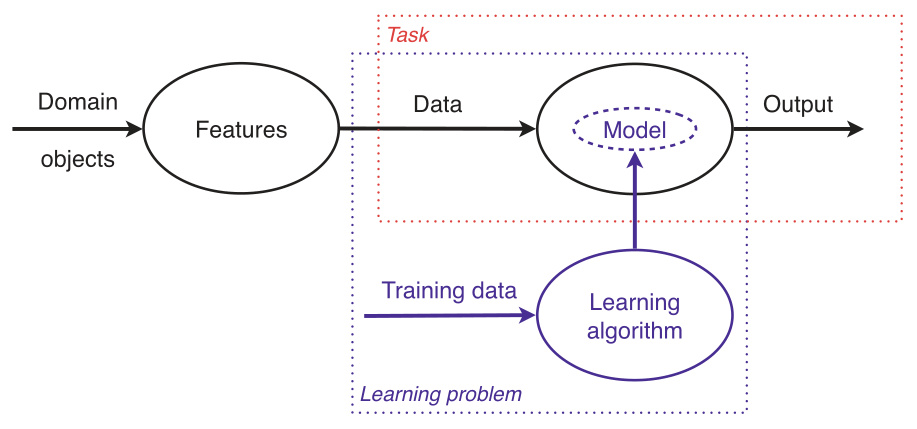
\includegraphics[width = 0.8\textwidth]{./Figures/machine_learning_peter_flach.jpg}
\rule{35em}{0.5pt}
\caption[Machine Learning]{Machine Learning is used to perform complex tasks. A task will require a mapping - a model - of inputs to outputs. The creation of the mapping by using sample data the model will encounter is a machine learning problem. }
\label{fig:machine_learning}
\end{figure}

%Kinds of Machine Learning
Machine Learning comes in three main categories; \textit{Supervised}, \textit{Unsupervised} and \textit{Reinforcement Learning}.
%Supervised
In Supervised Learning the algorithm is provided with many examples of input and the desired output for training.
To be more precise, given a set of data $D = ((\vo{x^n}, y^n), n = 1, ..., N )$, the algorithm must learn the relationship between the input vector $\vo{x}$ and the output $y$.
$\vo{x}$ is a vector of $m$ values, $\vo{x} = (x_1, x_2, ..., x_m)$ and $y$ is the corresponding output\citep{domingos2012few}.
A trained model can then take new input $\vo{x^\star }$ and predict the correct output $y^\star$.
We measure the degree of predictive success with the \textit{cost function}, $C(y^{pred}, y^{true})$, which takes the predictions and correct output as parameters.
Training the model is done by minimizing the cost function with respect to the model parameters.

%Supervised: Regression 
Supervised Learning itself has two sub-types - \textit{Regression} and \textit{Classification}.
Regression problems are concerned with giving real-valued output as a function of the input\citep{sammut2011encyclopedia}, see Figure ~\ref{fig:regression}.
There are many applications requiring numerical predictions on a continuum such as stock prices, temperatures and power generation.
\begin{figure}[htbp]
	\centering
		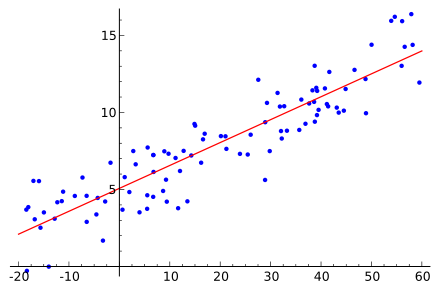
\includegraphics[width = 0.8\textwidth]{./Figures/regression.png}
		\rule{35em}{0.5pt}
	\caption[Regression]{In Regression a continuous output as a function of the features is learned. Here the examples (blue dots) have an output shown on the $y-axis $ as a function of a single feature, corresponding to the $x$-axis. While the examples clearly have the unmistakable pattern of an ascending straight line the regression model must be confused by the noise. The fitted model (shown in red) can be used to make predictions, $y_{pred} $, for the output of a new example input, $x^\star $, that is close to the true output of $y^\star $.}
		\label{fig:regression}
\end{figure}

%Supervised: Classification
Classification is predicting classes having learned from examples.
For example, a bank may wish to classify loan applicants into `high-risk' and `low-risk' groups.
Unlike regression, the output $y$ can only take on the discrete values of `high-risk' or `low-risk'.
A model is built from the customers' historical data of income, savings, professions, ages and debt histories that can predict the risk class of a new applicant.
These items of information about the applicant are known as \textit{features}.
If we look into the \textit{feature space}, a space made with each feature as a spacial dimension, we can create a model that separates the two classes, see Figure ~\ref{fig:classification}.
Features relevant to an applicant's financial capacity can provide many weak relations associated with their loan risk\citep{alpaydin2004introduction}.

This resulting model can also be analysed to reveal the data's underlying structure.
In the bank example, researchers can find common attributes of low-risk customers useful for target advertising for new and safe loans.
\begin{figure}[htbp]
	\centering
		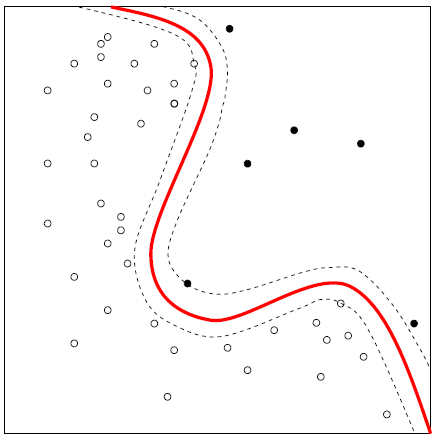
\includegraphics[width = 0.4\textwidth]{./Figures/classification.png}
		\rule{35em}{0.5pt}
	\caption[Classification]{Two different classes (circles and dots) fill the two dimensional feature space. Classification is the building of a model that can separate the classes such that for any new feature vector, $x^\star$, the correct class can be predicted. The model shown by the red line cuts across the feature space to differentiate the class of objects on one side versus the other.
	This algorithm used here tries to produce a boundary that is equally distant between the nearest examples, as shown by the broken lines to either side of the border. If a new object which lies to the top-right of the feature plane were discovered the model can be used to predict that it should be a dot. }
		\label{fig:classification}
\end{figure}

A regression model can tackle classification problems by assigning a level of confidence for an object belonging to a class.
This is often done by giving a prediction between zero and one.
The continuous output is then discretized, often by thresholding, to get a discrete label.
For example, output above 0.5 would be classified as a cat and below 0.5 as a dog.
Multi-label problems however cannot be answered by a single-valued output.
A classic example used within machine learning texts\citep{lecun2007mnist} is that of optical character recognition; recognizing printed or written numeric characters from their scanned images.
Such multi-label problems are treated by producing an output vector, $\vo{y}$, of ten values between zero and one.
Should the second value in the vector be the largest this would mean the digit is classified as a two.
The vector $\vo{y}_i = (0, 1, 0, 0 , 0, 0, 0, 0, 0, 0)$ would symbolise the label as being a two as the $1$ is in the second position.
Similarly $\vo{y}_i = (0, 0, 1, 0, 0, 0, 0, 0, 0, 0)$ represents a three.
This method of numerically encoding discrete labels is known as \textit{one-hot encoding}.

%Unsupervised Learning
Ideally machines would learn about the world as babies in that they learn to distinguish objects and people without being given explicit labels.
Machine Learning could then be much more useful as there is far less labelled data.
Learning models without data labels is known as \textit{Unsupervised Learning}.
Unsupervised algorithms attempt to find an accurate but compact description of the data\citep{barber2012bayesian}.
Once built, the model can be used to find clusters, as in Figure ~\ref{fig:Clustering}, compress the data or generate more with the same structure.
%[show this twice, once without colour] 
\begin{figure}[htbp]
	\centering
		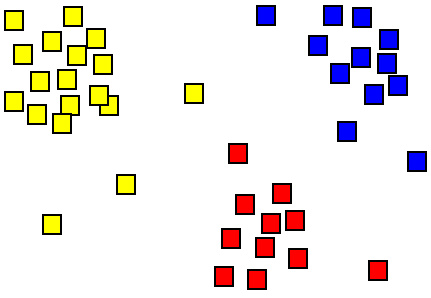
\includegraphics[width = 0.5\textwidth]{./Figures/clustering.jpg}
		\rule{35em}{0.5pt}
	\caption[Clustering]{While data may not have labels, Unsupervised Learning may still be used to uncover some inherent structure. Here indistinguishable objects, shown as squares, are in the two dimensional feature space. A common Unsupervised Learning method of \textit{Clustering} may be used to uncover how many clusters there are within the data and where in the feature space they lie.}
		\label{fig:Clustering}
\end{figure}

Semi-supervised learning is the common scenario in which there is little labelled but plenty unlabelled data.
For example, there are many millions of images of trees on the internet, but few of the images will specify the species.
Pure Supervised Learning would be forced to use only the labelled images and cast away the rest, losing valuable information.
Semi-supervised learning takes a more advanced approach and uses the unlabelled data to enhance the learning process.
The unlabelled data is used to `prime' the model, narrowing in on a range of useful parameter initializations before supervised learning begins.
The \textit{pre-training} makes the model come to recognize trees, even though it cannot yet distinguish species.
It will come to expect trunks, branches, green leaves and bark.
From there, the subtleties of variations that distinguish species can then be taught using the limited labelled data.
The final model will generally be better than one trained on the labelled data alone as shown in Figure ~\ref{fig:Unsupervised_learning}.
\begin{figure}[htbp]
	\centering
		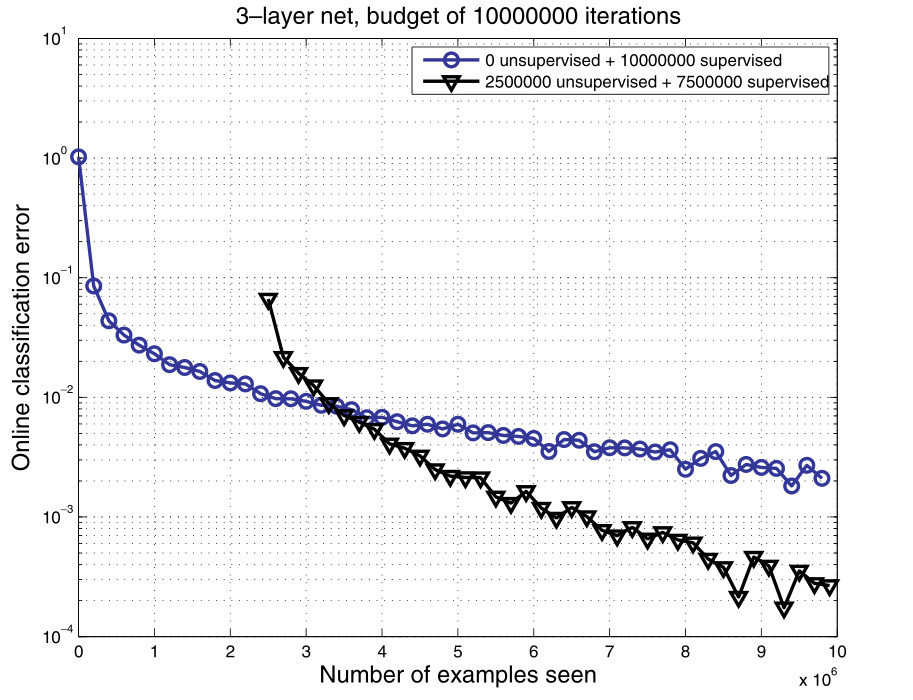
\includegraphics[width = 0.8\textwidth]{./Figures/Learning_deep_architectures_for_AI_Bengio_unsupervised_learning.jpg}
		\rule{35em}{0.5pt}
	\caption[Semi-supervised Learning]{A semi-supervised model (shown in black) was shown 2.5 million examples without labels. These were used to instantiate the model parameters with better starting values than randomness would have produced. In this case, the semi-supervised model outperforms the supervised model (shown in blue), with parameters settled on sub-optimal values due to the worse initialised parameter values. Analogously it is much easier to teach someone to recognize different bird species (the labels) when they are accustomed to what birds generally look like. The oscillations to the far right of the semi-supervised model result from the error being so close to zero that sampling variations appear large on the log-scale.}
	\label{fig:Unsupervised_learning}
\end{figure}

Instead of predicting output or uncovering structure, \textit{Reinforcement Learning} handles an agent in an environment, like a character in a game world.
The object is to maximize the agent's behaviour - its actions in response to its environment - when a reward is received over time or only at the very end.
Figure ~\ref{fig:Reinforcement _Learning_2} shows an AI system that can learn to play Atari games without explicit instructions at all.
Unlike Supervised Learning the agent is not informed of correct and incorrect behaviours but unlike Unsupervised Learning there is some feedback on performance.
If the game character's reward is its survival time it must learn life-span enhancing behaviour, such as eating, and avoiding dangerous actions, like drinking poison.
\citep{barber2012bayesian}

\begin{figure}[htbp]
	\centering
		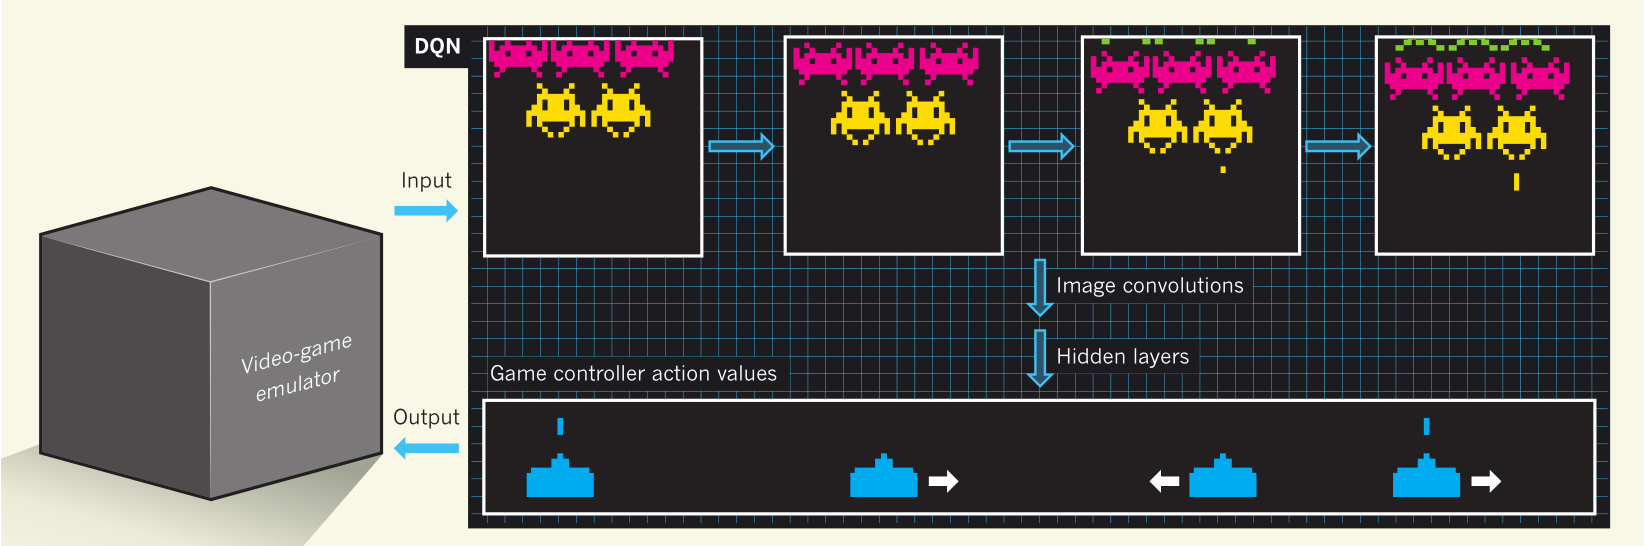
\includegraphics[width = 1.0\textwidth]{./Figures/Reinforcement_Learning_Learning_to_see_and_act.jpg}
		\rule{35em}{0.5pt}
	\caption[Reinforcement Learning]{The `Deep Q-Network' analyses four sequential video frames and predicts future game score for each possible action. This system is not even given instructions as to what objects to avoid, the characteristic elements of the game or how each control will impact the score. Instead information is extracted from the pixels through image convolutions and hidden layers [described in Section ~\ref{sec:neural_networks}] and fed to the Reinforcement Learning algorithms which must learn to recognize game elements and their attributes and which actions in different game states most improve the score.}
	\label{fig:Reinforcement _Learning_2}
\end{figure}

Sometimes new information becomes available over time. 
This means the model would have to be entirely retrained on the expanded data-set, a time-consuming task. 
\textit{On-line learning} is used to combat this problem.
Predictions are made on each instance in a series and it will receive a reward or loss after each one\citep{sammut2011encyclopedia}.
It is not necessarily supervised or unsupervised as incoming data may or may not have labels.
The model's objective is to maximise accumulated reward (or minimize the accumulated loss).
Expressed formally:
For each item in the sequence $s = 1, 2, 3, ...$, the algorithm:
\begin{enumerate}
\item Takes input $x_s \in X$
\item Makes prediction $y_s \in Y$
\item Receives a response $z_s \in Z$
\item Incurs a cost $c_s = c(y_s, z_t)$
\end{enumerate}
On-line learning is similar to reinforcement learning however the reward is instantaneous.

\subsection{Features}
%Features:Binary/Nominal/Continuous
In all machine learning applications features come in three types.
\textit{Binary Features} can take on only True or False values (numerically represented as $1$ and $0$).
For instance a feature `being human' can only be true or false.
\textit{Nominal Features} are multi-valued but discrete, such as a person's shoe size.
\textit{Real Features} can take on a continuous range of values such as someone's height.

%Features:correlated redundant irrelevant 
Not all features are equally useful for a machine leaning practitioner.
Some features are irrelevant and only serve to add noise to the data-set which can decrease performance.
A person's favourite colour would likely not help predict their income.
Correlated features are ones that are related to each other.
For example a person's weight is strongly correlated with their height.
As a person's height increases, their weight usually does too.
Including their weight to the feature-set would add information but not as much as an uncorrelated (but relevant) feature would.
Lastly, a feature may be entirely redundant (a correlation coefficient of 1 or -1) adding no new information that is not already captured in the data.
For example, a copied column of useful features would be relevant but redundant. 

\section{Neural Networks}\label{sec:neural_networks}
%Introduction
%History Outline
%The perceptron (natural comparison)
%Activation Function
%Networking Perceptrons
%MLPs

%Introduction
\textit{Artificial Neural Networks} (ANNs) are one of many Machine Learning algorithms used.
In Deep Learning applications, which we shall cover in Section ~\ref{sec:deep_learning}, ANNs are almost exclusively used.
For us they will make an indispensable start toward Deep Learning techniques and serve as a platform for more in-depth ML understanding.
A simple definition of an ANN was provided by an influential figure in neuro-computing, Dr. Robert Hecht-Nielson.
He defines a neural network as ``\textit{...a computing system made up of a number of simple, highly interconnected processing elements, which process information by their dynamic state response to external inputs}"\citep{caudill1989neural}.
ANNs derive their name from being simplistic models of biological neural networks found within brains, see Figure ~\ref{fig:Biological_Neuron} 
\begin{figure}[htbp]
	\centering
		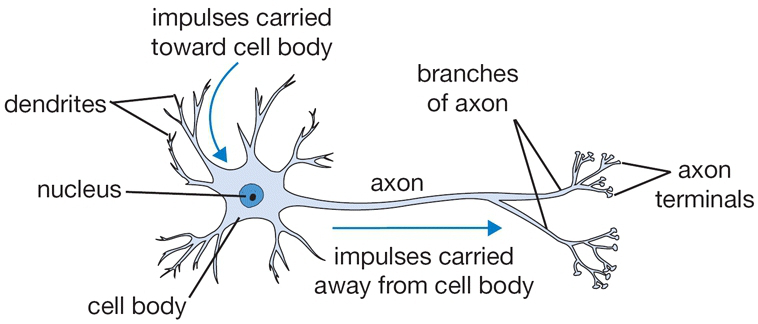
\includegraphics[width = 0.7\textwidth]{./Figures/neuron.png}
		\rule{35em}{0.5pt}
	\caption[Biological Neuron]{ANNs are loosely inspired by the structure and operation of biological neurons. The neuron receives information in the form of of potential differences at the tips of the dendrites. These electrical impulses are then carried toward the cell body which will itself emit an electrical signal along the axon to other neurons. The emission of an electric spike is dependent on the information received at the dendrites and the `chemical computation' of those inputs within the cell. Biological neurons either fire or they do not, but do not emit a continuous range of potential differences as an artificial neuron does.}
	\label{fig:Biological_Neuron}
\end{figure}

%History Outline
The first neural network model was developed with electrical circuits by Warren McCulloch and Walter Pitts in 1943\citep{mcculloch1943logical}.
However the model lacked a mechanism for learning.
Since then there have been many improvements\citep{bengio2009advances}.
The advent of significantly faster computers in the 50's allowed for larger networks\citep{bengio2009advances} leading IBM to form a research group to study pattern recognition and information theory under the leadership of Nathaniel Rochester\citep{bengio2009advances}.
They developed and simulated abstract neural networks on the new IBM 704 computer.
By 1959 neural network models called ``ADALINE" and ``MADELINE'' were designed that were similar to the ANNs of today\citep{bengio2009advances}.
MADELINE was more advanced than her counterpart and was the first ANN applied to solve a real problem; eliminating echoes on phone lines.
Then in 1962 a significant step was made; a learning algorithm, the Windrow-Hoff rule, was developed that could change parameter values as a function of the prediction error\citep{bengio2009advances} making the neuron perform better.

Despite the promising success with neural networks, interest faded in favour of Von Neumann computing architecture in a period known as the \textit{AI winter}\citep{kurzweil2014singularity}. 
This was partly the result of the early successes which led to over-expectations for what neural networks are capable of.
The inevitable disappointment led to research and funding being drastically decreased.

In 1986 three independent research groups tackled a method to extend the Windrow-Hoff rule to multi-layer networks and came up with similar ideas regarding the what is now called \textit{back-propagation} 
The development of this powerful training algorithm combined with faster computers thawed neural networks out of obscurity.

%The perceptron (natural comparison)
No understanding of neurons would be complete without first understanding \textit{Perceptrons}\citep{mo2012survey}.
Developed in the 50's and 60's by Frank Rosenblatt, a perceptron consists of one or more inputs, a processor and a single output\citep{mo2012survey} illustrated in in Figure ~\ref{fig:Perceptron}.
The flow of information follows a ``feed-forward model".
This means $m$ inputs, represented by the real-valued $\vo{x} = (x_1, x_2, x_3, ... , x_m)$, are fed to the perceptron which computes a single result.
Each input value, $x_i$, is multiplied by a corresponding real-valued \textit{weight} $w_i$ when grouped forming a real-valued weightings vector $\vo{w} = (w_1, w_2, w_3, ..., w_m)$.
All weighted inputs are summed, which can be represented as a dot-product
\be
\sum^m_{i = 1} x_i w_i = \vo{x} \cdot \vo{w}
\ee
where $m$ is the number of inputs.
Should the sum be greater than the threshold $0$, the perceptron outputs a $1$, otherwise a $0$.
Expressed as a function this reads,
\be
    f(\vo{x}) = 
\begin{cases}
   	1	,		& \text{if } \vo{x} \cdot \vo{w}\geq 0\\
    0	,     	& \text{otherwise}
\end{cases}
\ee
The larger the absolute value of a weighting $|w_i|$ the more the corresponding input $x_i$ contributes to the sum.
A positive weighting increases the likelihood of `exciting' the neuron which leads to an output of $1$.
Negative weights will reduce the sum and so `inhibit' the neuron.
Weightings can be tuned so the neuron is more responsive to specific inputs, some of which will be excitatory and others inhibitory.
Similarly changing the threshold affects the output but in the reverse manner to the weightings.
\textit{Decreasing} the threshold increases the likelihood of the neuron `firing' whereas increasing the threshold decreases the likelihood.
Threshold varying is equivalent to holding the threshold constant and adding a \textit{bias}, a constant $b$, to the dot-product.
\be
    f(\vo{x}) = 
\begin{cases}
   	1	,		& \text{if} \vo{x} \cdot \vo{w} + b \geq 0\\
    0	,     	& \text{otherwise}
\end{cases}
\ee
A positive bias is then excitatory, and negative is inhibitory.
This still is not optimal as now weightings and an additional bias term must be tuned.
Instead the bias is absorbed into the dot-product by introducing an extra input of $x_0$ which is always equal to one with its corresponding weighting of $w_0$.
By varying the weighing $w_0$ this is equivalent to changing the value of the bias term.
Now all neuron tuning is done on the weightings.

%Activation Function
Till now we made the neuron output only a zero or one according to a threshold.
There is no reason why the output cannot be some other function $f(\vo{x} \cdot \vo{w})$, known as the \textit{activation function}.
Many different activation functions have been used throughout ANN's development.
The function favoured today is the Rectified Linear Unit (ReLU) or $max(0, X)$.
ReLU activations will grow linearly for $X > 0$ but are $0$ where $X < 0$.
Research has shown they make training quicker and have better overall results\citep{NIPS2012_4824}.

%Networking Perceptrons
A perceptron can learn a limited number of relations between inputs\citep{mo2012survey}.
In particular the exclusive-or (XOR) function is beyond its learning capability as shown in 1969 by Marvin Minsky and Seymour Papert\citep{minsky1969perceptrons}.
However the output of one neuron may fed as the input to another neuron and so on forming a network.
Combining many simple elements into a network can produce a much more complex system\citep{bar1997dynamics}.
Networks differ in kind but all share the same components: \textit{nodes}, and connections between them\citep{gershenson2003artificial}.
Individual nodes can be thought of as computational units or neurons.
Each receives input and processes the information to generate an output.
The processing may be very basic (such as a simple summation of the input) or more complex.
Connections between the nodes determine the direction of information flow.
Interactions between the nodes lead to the complex emergent behaviour of the network.
\begin{figure}[htbp]
	\centering
		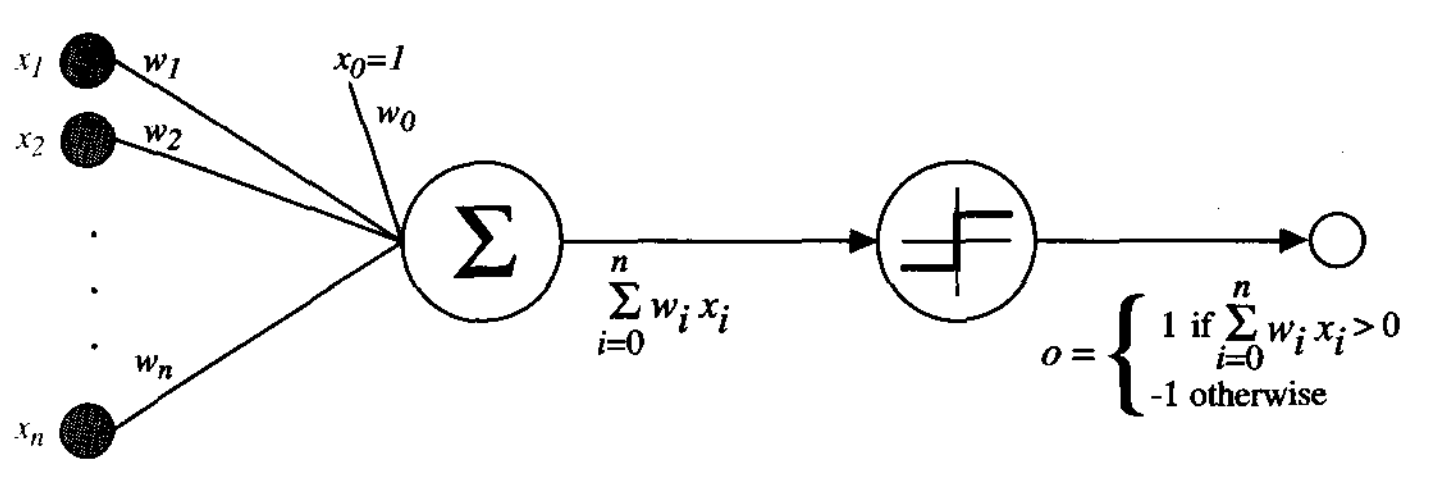
\includegraphics[width = 1.0\textwidth]{./Figures/ML_tom_mitchel_perceptron.PNG}
		\rule{35em}{0.5pt}
	\caption[The Perceptron]{A Perceptron is a simple model of a neuron. Input is given in the form of a linear weighted sum, $\sum^n_{i = 0} w_i x_i$, over all $n$ input values. The result is used as input for the (often non-linear) \textit{activation function}. For the first perceptrons this was the step-wise function which outputs $1$ if the sum is greater than $0$, otherwise a $-1$}
	\label{fig:Perceptron}
\end{figure}

%MLPs
\begin{figure}[htbp]
	\centering
		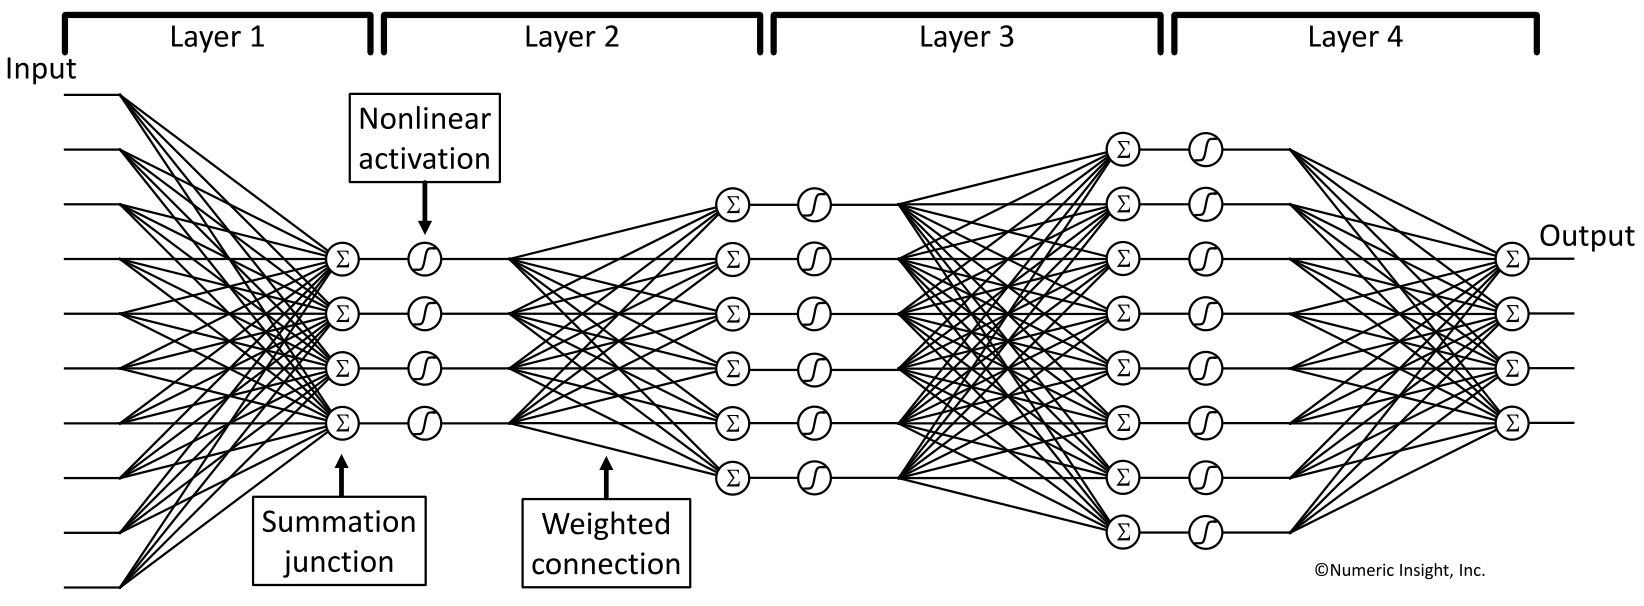
\includegraphics[width = 1.0\textwidth]{./Figures/MLP_a_survey_time_travel_in_DL_4.jpg}
		\rule{35em}{0.5pt}
	\caption[Multi-Layer Perceptron]{Pictured above is the architecture of a Multi-Layer Perceptron (MLP). An MLP is an example of a `feed-forward' network as information flows through the network in one direction only (left to right in the figure). The network is composed of an arbitrary number of layers but will always have an \textit{input layer} (on the far left) which receives the features and an \textit{output layer} (on the far right) which returns the model results. Each perceptron within Layer 1 takes a weighted sum - connection weightings can differ between neurons - of the input features through a non-linearity (often a sigmoidal function). The singular output of each input node forms one feature for the next layer to the right, the first \textit{hidden layer}. Similarly output from each of the Layer 2 neurons serves as input features to Layer 3, the second hidden layer. Finally layer 4, the \textit{output layer}, computes the model result. As there are four output nodes, this MLP provides four different answers. For example each of the four neurons may give output representing the model's confidence that the input example image features belong to a cat, dog, man or mouse respectively. The Layer 4 neuron with the largest output will then determine to which of the classes the item belongs. }
	\label{fig:MLP}
\end{figure}
Feed-forward ANNs, are organized into layers.
There are at least two layers to a neural network such as in Figure ~\ref{fig:MLP}; the first layer, or \textit{input layer}, and the last layer, the \textit{output layer}.
Should there be layers between, they are known as \textit{hidden layers}.
The output from all input layer neurons are fed as input to second layer neurons.
The second layer's output is now based on the results from the input layer.
A feed-forward system allows proceeding layers make decisions at a more abstract level than preceding layers\citep{krose1993introduction}.
These networks are much more capable of fitting to arbitrary feature relations.
In fact they can compute any continuous function\citep{hornik1989multilayer}.
Changing one neuron to act as an AND logic gate is easily done by hand.
However for ANNs that have hundreds or thousands of neurons an algorithm must be used to train the weightings.

\subsection{Training}
%backpropogation
	%Last Layer
	%Hidden Layers
%SGD
%Momentum, Adagrad etc..
%Learning Decay
%Activation Fucntions
%Weight Initialization
%Batch Norm
%Final layer norm
%GPU acceleration

%Regularization
	%Dropout
	%Early Stopping

Geoffrey Hinton, around 1985, developed a multi-layer neural network that could learn more functions than the single layer perceptron could\citep{mo2012survey}\citep{williams1986learning}.
Hinton also developed the training algorithm for multi-layered neural networks called \textit{back-propagation}\cite{mcclelland1986parallel}.
Back-propagation is a supervised learning training method whereby the cost is calculated.
The cost is a measure of the difference between output nodes of the network and their target values.

Mean Squared Error (MSE) is a common cost function used in regression models.
It is just the difference between the true value of example $i$, $y_i$, and the predicted value, $y_i^\star$.
\be
MSE = \frac{\sum^n_{i = 1}(y_i - y_i^\star)^2}{n} 
\ee
where $n$ is the number of examples in the test set, $y_i$ is the true label for example $i$, and $y_i^\star$ is the predicted value,

Back-propagation is aptly named as the cost is propagated backward though the network, adjusting connection weightings, or moving to a different location in `weight space' to reduce the error at every stage.
%\begin{figure}[htbp]
%	\centering
%		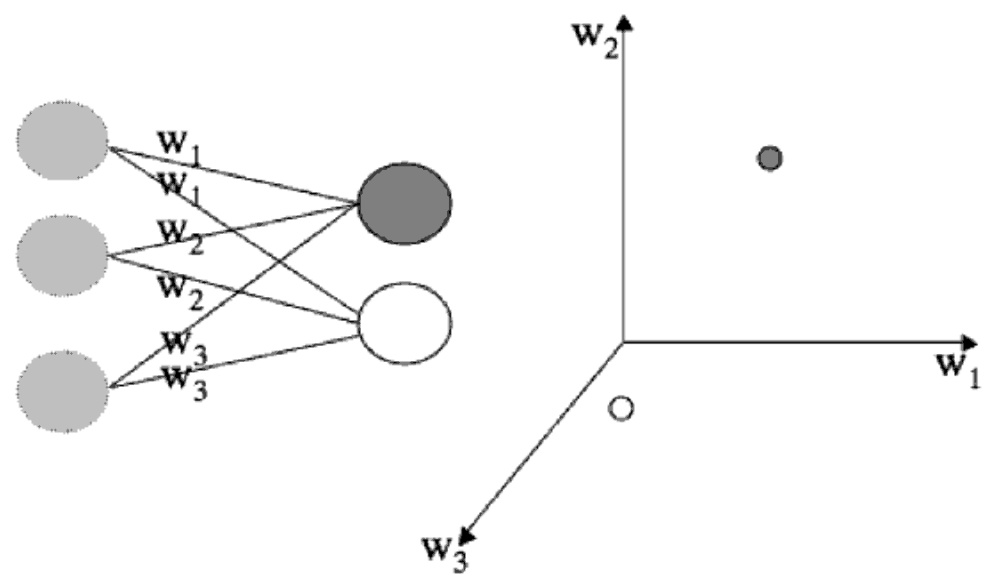
\includegraphics[width = 0.5\textwidth]{./Figures/machine_learning_an_aglorithmic_perspective_weight_space.jpg}
%		\rule{35em}{0.5pt}
%	\caption[Weight Space]{All the parameters in a model can be thought of as dimensions of `Weight Space'. All weightings of a neural network are represented by a single point in weight space. The objective of model training is to move this point in weight space from where it is currently located (in gray) to one in which the network makes better predictions (outlined).}
%	\label{fig:Weight_space}
%\end{figure}
\begin{figure}[htbp]
	\centering
		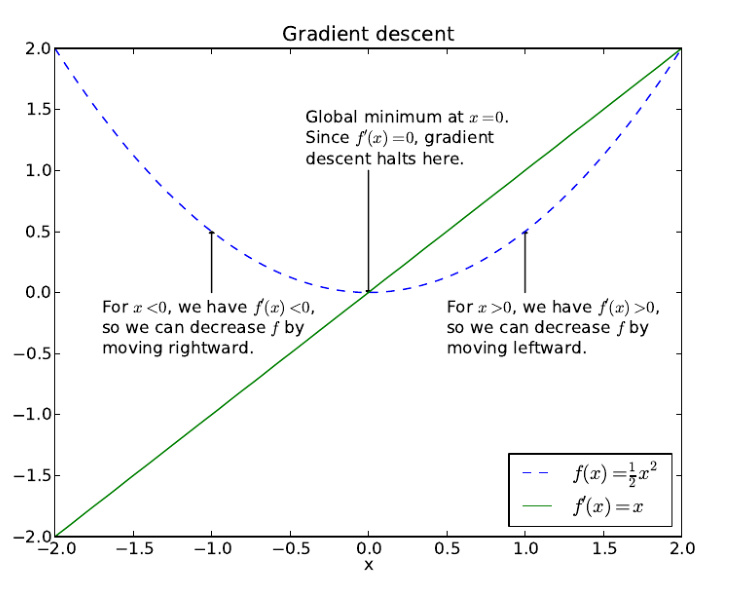
\includegraphics[width = 0.8\textwidth]{./Figures/gradient_descent_DL_textbook_8.jpg}
		\rule{35em}{0.5pt}
	\caption[Gradient Descent]{A neural network like many machine learning models can be highly complex, non-linear and non-convex. 
A function, $f(x)$, is convex over an interval $[a, b]$ if the second derivative $f^{\prime \prime}(x) \geq  0$ for all $x$ in $[a, b]$.
It may not be possible to analytically calculate the optimal parameters for the model. However we can use gradient descent to slide down the surface of the cost function to a minima. Consider the simplified cost equation of $f(x) = \frac{1}{2}x^2$. Left of the minima at $x = 0$ the derivative, $f^\prime(x) = x$, will be negative. So we can decrease the value of $f(x)$ by choosing a new value for $x$ to the right of its previous position. Similarly where $x$ is positive the derivative will be positive and so moving leftward will bring us closer to the minima.}
	\label{fig:Gradient_descent}
\end{figure}
\begin{figure}[htbp]
	\centering
		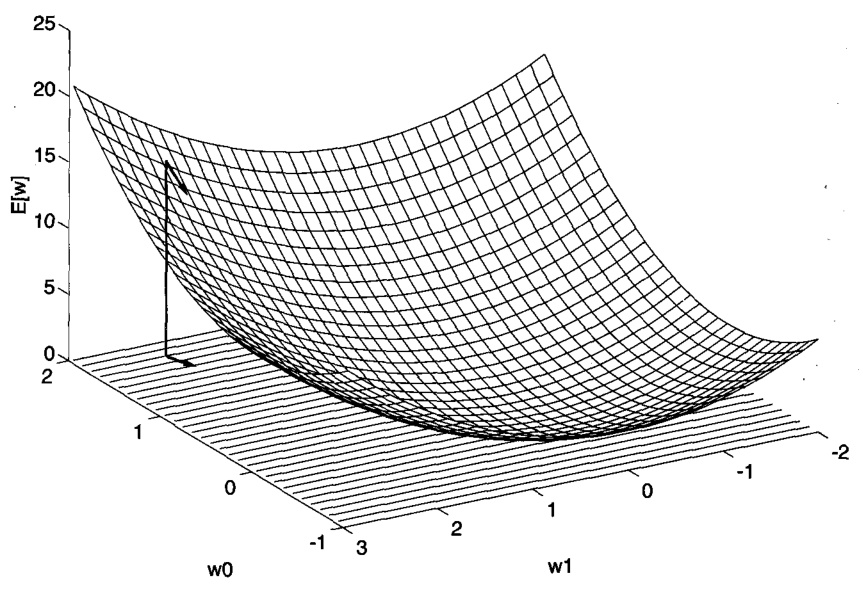
\includegraphics[width = 0.6\textwidth]{./Figures/ML_tom_mitchel_gradient_decent.jpg}
		\rule{35em}{0.5pt}
	\caption[Multi-dimentsional gradient descent]{Where the cost function is a surface in a multidimentsional space, here $w0$ and $w1$, the negative of the derivative at any point will point in the direction of steepest decent. Updating the weights to new values close to the last position but in the direction of steepest descent will reduce the cost of the model.}
	\label{fig:Gradient_descent_2}
\end{figure}

\textit{Gradient descent} is the method used to tune the weights once we have the cost.
The cost function can be pictured as a surface of height parametrised by the weightings, see Figure ~\ref{fig:Gradient_descent} for a detailed picture.
The cost-surface will have many peaks, local maxima, and troughs, local minima.
Weights are usually initialized to take on random values; the exact distribution from which they are sampled can vary.
All the weight co-ordinates will specify a point in the cost-landscape.
The lowest possible cost, and so the best fit of the neural network, lies in the deepest trough, the global minima.
Gradient descent looks at the immediate area around the current location, see Figure ~\ref{fig:Gradient_descent_2}, and walk down the path of steepest descent.
As gradient descent only walks downhill, and not up, there is no guarantee that it will reach the global minima.
Gradient descent cannot climb a peak to get to a deeper trough.
Finding the gradient of a function is in principle straight forward but can get messy.
First lets define some notation referring to Figure ~\ref{fig:MLP_2}:
$z_j$ is the weighted input sum of node $j$ in layer $l$.
$g_j$ is the activation function applied to $z_j$ at node $j$ in layer $l$.
$a_j$ is the activation, the output of $a_j = g_j (z_j)$ at node $j$ in layer $l$.
$w_{ij}$ is the weight connecting node $i$ in layer $(l-1)$ to node $j$ in layer $l$.
$t_k$ is the target prediction for the $k$'th neuron in the output layer.

\begin{figure}[htbp]
	\centering
		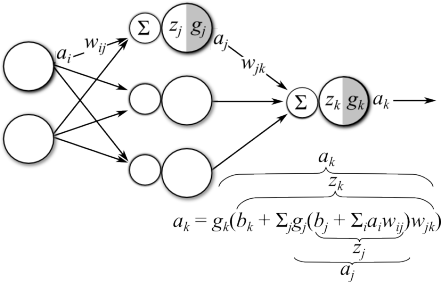
\includegraphics[width = 0.7\textwidth]{./Figures/neural_net.png}
		\rule{35em}{0.5pt}
	\caption[MLP Notation]{The effective algebraic function of an MLP takes the form of activation functions nested inside each other. Input activation values, or features, $a_i$ are used in the weighted summation, $z_j = b_j + \sum_i a_i w_{ij}$, as part of the input to the next activation function, $g_j$, which determines the activation, $a_j = g_j(z_j)$. These values are in turn used in the weighted sum, $z_k = b_k + \sum_j a_j w_jk$ as input to the final activation function, $g_k$, to produce the activation of $a_k$. If the model parameters are tuned correctly $a_k$ should be close to the true output, $t_k$, corresponding to input features $a_i$. The training method of back-propagation uses the chain-rule of calculus to see what the effect a slight change to each parameter would make to the final result. The model will then update each parameter in the direction that to first-order brings the output closer to the true value\citep{backpropagationImage}.}
	\label{fig:MLP_2}
\end{figure}

%Last Layer
To take you through the back-propagation algorithm we will consider a \textit{Multi-Layer Perceptron} (MLP) with one hidden layer.
The first case we will look at is the weights connecting the final hidden layer to the output layer.
Nodes in the hidden layer are indexed by $j$, where there are $J$ nodes in the final layer.
The $K$ output nodes are similarly indexed by $k$.
For the cost function we will the squared difference between target values and the network predictions.
This is often used in regression problems, here we use it for simplicity.
The cost function $C$ is therefore
\be
C = \frac{1}{2}\sum_{k\epsilon K} (a_k - t_k)^2
\ee
A factor of $\frac{1}{2}$ does not affect the results and is used for later convenience.
The function returns the cost of a single feed-forward prediction relating to a single example's features.
The total cost is the sum of every individual prediction's cost.
This is because we do not wish to make the network very good at recognizing only one item, but instead predict very well on the whole data set.

We can use the chain rule to calculate the gradient of the cost with respect to each weight, $w_{ij}$.
\be
\begin{aligned} \label{eq:cost_derivitive}
\frac{\partial C}{\partial w_{jk}} 	&= \frac{\partial}{\partial w_{jk}} \left(\frac{1}{2} \sum_{k\epsilon K} (a_k -t_k)^2\right)\\
									&= (a_k-t_k)\frac{\partial}{\partial w_{jk}} (a_k -t_k)\\
\end{aligned}
\ee
We drop the summation as only one term survives the differentiation.
The weight $w_{jk}$ connects the $j'th$ neuron in layer $l-1$ to only the $k$th output node therefore every other output node has no dependence on $w_{jk}$ and so all other derivatives are zero.
Looking at the partial derivative in Equation ~\ref{eq:cost_derivitive} we get
\be
\frac{\partial C}{\partial w_{jk}} = (a_k-t_k)\frac{\partial}{\partial w_{jk}} (a_k)
\ee
since $t_k$ is independent of the weights.
Now we use the chain rule again on the activation $a_k = g_k (z_k)$
\be
\begin{aligned} \label{eq:z_d_w}
&= (a_k-t_k)\frac{\partial}{\partial w_{jk}} [g_k (z_k)]\\
&= (a_k-t_k) g_k^\prime (z_k) \frac{\partial}{\partial w_{jk}} z_k
\end{aligned}
\ee
The weighted sum in the output layer is given by $z_k = \sum_{j\epsilon J} g_j (z_j)w_{jk}$.
Taking the partial derivative we get $\frac{\partial z_k}{\partial w_{jk}} = g_j (z_j) = a_j $.
Again only one term survives from the summation, but this time of index $j$.
Substituting this simple result in place of $\frac{\partial z_k}{\partial w_{jk}}$ in Equation ~\ref{eq:z_d_w} we have 
\be
\frac{\partial C}{\partial w_{jk}} = (a_k-t_k) g_k^\prime (z_k)a_j
\ee
where $g_k^\prime$ is shorthand for $\frac{\partial g_k(z_k)}{\partial w_{ij}}$.
We see the derivative is a product of three terms:
The difference between prediction and target value of neuron $k$; second is the derivative of node $k$'s activation function from the last layer; lastly is the activation of node $j$ in the previous layer.
Grouping all terms involving $k$ under $\delta_k$ we get
\be
\frac{\partial C}{\partial w_{jk}} = \delta_k a_j
\ee
where
\be
\delta_k = (a_k-t_k) g_k^\prime (z_k)
\ee
The $\delta_k$ can be thought of as a measure of the error at $t_k$.
The error is back propagated to all the weights $w_{1k}, w_{2k}, w_{3k}, ... , w_{Jk}$ in proportion to activation values $a_1, a_2, a_3, ... , a_J$.
In doing this we find each weight's contribution toward the error we wish to minimize.
So we now update the weights as $w_{jk}\leftarrow w_{jk} - \eta \frac{C}{w_{jk}}$ where $\eta$ is the magnitude of the step, or the \textit{step size}.
For all $N$ examples within the data-set we sum the $N$ steps $\eta \frac{C}{w_{jk}} $ so as to average the best possible step to minimize the total cost.
Too small a step size means the algorithm will take too long to converge, and perhaps get stuck in local minima.
Too large a step size and gradient descent can overshoot minima altogether, or oscillate over the minima never settling in the local minima, see Figure ~\ref{fig:global_and_local_minima} for better understanding.
\begin{figure}[htbp]
	\centering
		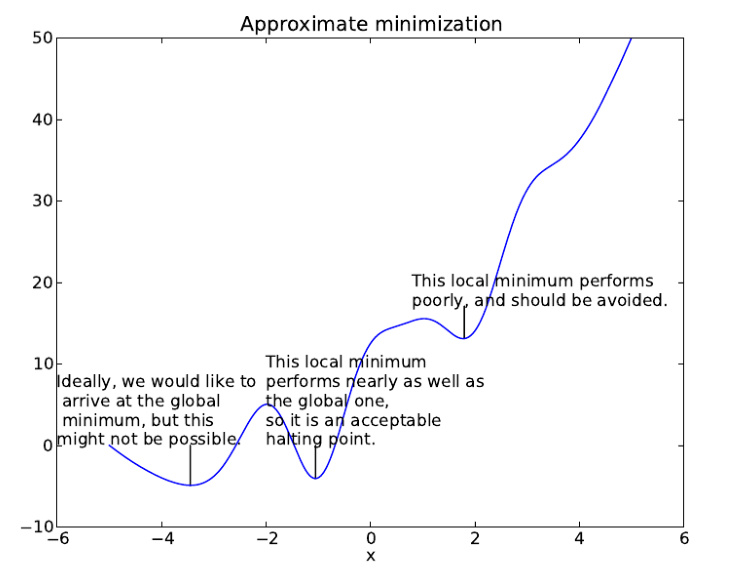
\includegraphics[width = 0.9\textwidth]{./Figures/global_verse_local_minimum_DL_textbook_9.jpg}
		\rule{35em}{0.5pt}
	\caption[Local Minima]{Navigating the cost function is not as simple as the case in Figure ~\ref{fig:Gradient_descent_2}. The surface will likely not have one local minima but many. Training the network by sliding down the cost surface can trap the model in a sub-optimal local-minima. The ideal is to find the global minima as in the image above, however this may be too hard to find. Therefore many local-minima which perform nearly as well as the global minima are acceptable halting points for training.}
	\label{fig:global_and_local_minima}
\end{figure}
%Middle Layer
We now proceed with how to update the weights for all layers other than the last hidden one.
Now $i$ indexes nodes in layer $(l-1)$ and $j$ those of layer $l$.
The derivative with respect to inner layer weights is
\be
\begin{aligned} \label{eq:dC_dw}
\frac{\partial C}{\partial w_{ij}} 	&= \frac{\partial}{\partial w_{ij}}\frac{1}{2} \sum_{k\epsilon K} (a_k -t_k)^2\\
									&= \sum_{k\epsilon K}(a_k-t_k)\frac{\partial}{\partial w_{ij}} (a_k)
\end{aligned}
\ee
This time the sum is not dropped as every node in the hidden layer affects every node in the output layer.
Substituting $a_k = g_k (z_k)$ into Equation ~\ref{eq:dC_dw} we obtain
\be
\frac{\partial C}{\partial w_{ij}}	= \sum_{k\epsilon K}(a_k-t_k) \label{eq:derivitive_into} g_k^\prime(z_k)\frac{\partial}{\partial w_{ij}} (z_k)
\ee
Now 
\be
\begin{aligned} \label{eq:Z_kDecompose}
z_k &= \sum_{j\epsilon J} a_j w_{jk}\\
	&= \sum_{j\epsilon J} g_j (z_j)w_{jk}\\
	&= \sum_{j\epsilon J} g_j \left(\sum_{i\epsilon I} z_i w_{ij}\right)w_{jk}
\end{aligned}
\ee

After decomposing $z_k$ in Equation ~\ref{eq:Z_kDecompose} we determine $\frac{\partial z_k}{\partial w_{ij}}$ with the chain rule.
\be
\begin{aligned}
\frac{\partial z_k}{\partial w_{ij}} &= \frac{\partial z_k}{\partial a_j} \frac{\partial a_j}{\partial w_{ij}}\\
 & = \frac{\partial}{\partial a_j}(a_j w_{jk}) \frac{\partial a_{j}}{\partial w_{ij}}\\
 & = w_{jk} \frac{\partial a_j}{\partial w_{ij}}\\
 & = w_{jk} \frac{\partial g_j(z_j)} {\partial w_{ij}}\\
 & = w_{jk} g_j^\prime (z_j)\frac{\partial z_j }{\partial w_{ij}}\\
 & = w_{jk} g_j^\prime (z_j)\frac{\partial }{\partial w_{ij}}\left(\sum_{i\epsilon I} a_i w_{ij}\right)\\
 & = w_{jk} g_j^\prime (z_j) a_i
 \end{aligned}
\ee
plugging in this solution for $\frac{\partial z_k}{\partial w_{ij}} $ into Equation \ref{eq:derivitive_into} we have
\be
\begin{aligned}
\frac{\partial C}{\partial w_{ij}} &= \sum_{k\epsilon K}(a_k-t_k) g_k^\prime(z_k) w_{jk}g_j^\prime(z_j)a_i\\
&= a_i g_j^\prime(z_j) \sum_{k\epsilon K}(a_k-t_k) g_k^\prime(z_k) w_{jk}\\
&= a_i g_j^\prime(z_j) \sum_{k\epsilon K} \delta_k w_{jk}
\end{aligned}
\ee

Again we see errors back propagate with the error signal now being
\be
\delta_j = g_j^\prime (z_j) \sum_{k\epsilon K}\delta_k w_{jk}
\ee
such that

\be
\frac{\partial C}{\partial w_{ij}} = \delta_j a_i
\ee

To update the weights at layer $l-1$ the error signal of layer $l$ is back-propagated and weighted by the activation $a_i$.

What is particularly convenient about back-propagation is that all the operations are easily vectorizable.
There are many programming modules that perform vectorized equations significantly faster than iterating through all weights in a layer.
Graphics processing cards have thousands of cores which can do many thousands of algebraic equations at one.
We will come to the use of graphics cards later.

We can express this as a pseudo algorithm.

For each example $n$ in the training set of $N$ in total\citep{neuralnetworkswebsite}
\begin{enumerate}
\item Feed forward through each layer $l = 2, 3, .., L$ with
\be
z^{x,l} = w^l a^{x, l-1}
\ee
where 
\be
a^{x, l-1} = g(z^{x, l})
\ee
\item Compute the error at layer $L$:
\be
\delta^{x ,L} = \Delta_a C_x \odot g^\prime(z^{x, L})
\ee
where 
\be
\Delta_a C_x = \left[\frac{\partial C}{\partial a^L_1}, \frac{\partial C}{\partial a^L_2}, \frac{\partial C}{\partial a^L_3}, ..., \frac{\partial C}{\partial a^L_J}\right]
\ee
The element-wise product e.g.
$
\begin{bmatrix}
    2  \\
    3  \\
\end{bmatrix}
\odot
\begin{bmatrix}
    6  \\
   	7  \\
\end{bmatrix}
=
\begin{bmatrix}
    2\times 6  \\
    3\times 7  \\
\end{bmatrix}
$
is denoted by $\odot$.
\item Back-propagate through layers $l = (L, L-1, L-2, ..., 0)$ and
compute the error
\be
\delta^{x,L} = \left[(w^{l + 1})^T \delta^{x, l + 1}\right]\odot g^\prime(z^{x, l})
\ee
\item Update all weights according to Gradient Descent
for each layer update the weights according to
\be
w^l \leftarrow w^l - \frac{\eta}{N} \sum_{n\epsilon N} \delta^{n,l}(a^{n, l-1})^T
\ee
Each sweep through the entire data set is called an \textit{epoch}.
\end{enumerate}

\subsection{Advanced Training Methods}

%Weight Initializations
%SGD, Momentum, Adagrad, learning decay
Training an MLP with back-propagation as it was originally designed can take a long time.
Every training iteration requires several time-consuming stages even with vectorized computation.
Each training example must be fed-forward through the network.
Then each error must be back-propagated through the network.
Finally all the weights must be updated.
And that is just one iteration.
Back-propagation may not converge for thousands.

%Gradient Descent = Batch Gradient Descent
Standard gradient descent computes the gradient of the cost function, $C(\theta)$ , with respect to the parameters $\theta$ for the entire training set.
This is known as \textit{Batch Gradient Descent} and where weights are updated according to the following rule,
\be
\theta = \theta - \eta \dot \Delta_\theta C(\theta)
\ee
As the gradients need to be computed for the entire training set this can be a very slow training process and may be limited by memory size.
Such training is guaranteed to converge to the global minimum for convex surfaces such as in Figure ~\ref{fig:Gradient_descent_2}, and to a local minimum for non-convex surfaces.
%Stochastic gradient Descent
\textit{Stochastic Gradient Descent} (SGD) differs from batch gradient descent in that the model parameters are updated for each example $x^{(i)}$ and label $y^{(i)}$
\be
\theta = \theta - \eta \dot \Delta_\theta C(\theta; x^{(i)}; y^{(i)}) \label{eq:updateEquation}
\ee
Batch training may perform redundant calculations in large datasets where there are similar examples.
SGD however, performs a single update at a time and is much faster and can be used for on-line training.
On average the gradient will point in the correct direction with much less computation.

%Mini batch gradient decent
\textit{Mini-batch gradient descent} learns from both SGD and batch training and instead performs an update for every batch of $n$ training samples.
\be
\theta = \theta - \eta \dot \Delta_\theta C(\theta; x^{(i:i + n)}; y^{(i:i + n)})
\ee
In this way the high variance of parameter updates from SGD is reduced and training is faster\citep{lecun2012efficient}.
Common batch sizes vary between 2 to 256 examples.
Mini-batch training is what is commonly employed for training neural networks.
The term SGD is often used to describe mini-batch training.

The stochastic nature of the batch means the batch gradient will often differ from the complete set.
While that seems to be counter-productive the occasional mis-step means it is possible to step over local minima and find a deeper one.
Fewer samples increases the random mis-steps allowing much more exploration of the parameter-space.
However using too few samples has the side-effect of increasing the training time.
Every batch loaded contributes to the memory overhead.
SGD will spend a lot of time randomly jumping through the parameter space it will take a long time to converge.
However, the likelihood of finding a deeper minima is increased.

Too many samples within the batch will dampen the stochastic effect.
The more samples in a batch, the less time each epoch will take.
For best results the order in which the examples are fed to SGD in each epoch should be randomized\citep{lecun2012efficient}.

%Momentum
\textit{Momentum} is a method that helps SGD navigate surfaces which curve more steeply in one direction than in another, see Figure ~\ref{fig:Momentum_2}\citep{bengio2012practical}\citep{werbos1990backpropagation}.

This is done by smoothing out the SGD updates by adding a weighted average of prior gradients
\be
\mu = \gamma \mu_{t-1} - \eta.\Delta_\theta C(\theta)
\ee
\be
\theta = \theta - \mu_t
\ee

where $\gamma$, a hyper-parameter, is usually set to 0.9.
The momentum term increases the step-size for dimensions where gradients tend to point in the same direction and reduces step-size for dimensions where gradients often change directions.
The idea is that it removes some of the noise and oscillations SGD has, especially in the directions of high curvature, see Figure ~\ref{fig:Momentum_2} for an illustration.

Other extensions like Adagrad by Duchi\citep{duchi2011adaptive}, Nesterov accelerated GD\citep{nesterov1983method}, Adadelta by Zeiler\citep{zeiler2012adadelta} and Adam by Kingma and Ba\citep{kingma2014adam} are known to work equally well, if not better than standard momentum in certain cases.
\begin{figure}[htbp]
	\centering
		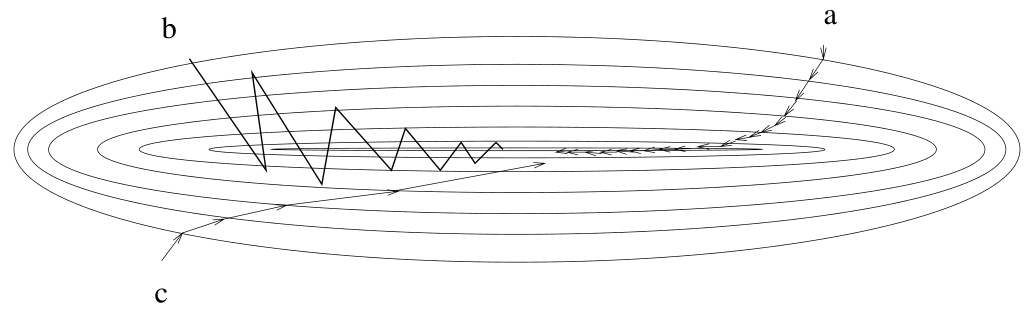
\includegraphics[width = 1.0\textwidth]{./Figures/momentum_An_introduction_to_NNs.jpg}
		\rule{35em}{0.5pt}
	\caption[Gradient Descent Comparisons]{The size of the step in weight space should be small enough so as to be in the region where the derivative is tangential to the surface, but too small and training may take a long time to converge, as in the case of path a. Too large a step-size will encourage the model to leap over the minima to the other side where the gradient has changed direction altogether. This leads to oscillatory behaviour, path b, where the model may never converge. Momentum, path c, starts with a small step-size, but increases the step size for the next iteration in the direction in which it last moved reaching the minima in much fewer steps.}
	\label{fig:Momentum_2}
\end{figure}

%Momentem Nesterov
Too much momentum will cause gradient descent to overshoot.
If the updates have a high momentum in one direction they will tend to overshoot the local minima repeatedly.
\textit{Nesterov Accelerated Gradient} tries to take into account the levelling off near the bottom in order to forcefully reduce the momentum.
If we use the momentum term $\gamma \mu_{t-1}$ to do the updates we can get an approximation for the next position by computing $\theta - \gamma_{t-1}$.
We can use this information to calculate the gradient not with respect to the \textit{current} parameters but with respect to the approximate future parameters:
\be
\mu_t = \gamma \mu_{t-1} - \eta \dot \Delta_\theta J(\theta-\gamma \mu_{t-1})
\ee
\be
\theta = \theta - \mu_t
\ee
where $\gamma$ will again be approximately 0.9.
%%adagrad
%\be
%g_{t,i} = \Delta_\theta J(\theta_i)
%\ee
%\be
%\theta_{t + 1,i} = \theta_{t,i} - \eta.g_{t,i}
%\ee
%\be
%\theta_{t + 1,i} = \theta_{t,i} -\frac{\eta}{\sqrt{G_{t, ii} + \epsilon}}.g_{t,i}
%\ee
%\be
%\theta_{t + 1} = \theta - \frac{\eta}{\sqrt{G_t + \epsilon}}\cdot g_t
%\ee
%%adadelta
%\be
%E[g^2]_t = \gamma E [g^2]_{t-1} + (1-\gamma)g_t^2
%\ee
%
%\be
%\Delta \theta_t = -\eta \dot g_{t,i}
%\ee
%
%\be
%\theta_{t + 1} = \theta_t + \Delta \theta_t
%\ee
%
%\be
%\Delta \theta_t = -\frac{\eta}{\sqrt{G_t + \epsilon}} \cdot g_t
%\ee
%
%\be
%\Delta \theta_t = -\frac{\eta}{\sqrt{E[g^2]_t + \epsilon}} g_t
%\ee
%
%\be
%\theta_t = -\frac{\eta}{RMS[g]_t}
%\ee
%
%\be
%E[\Delta \theta^2]_t = \gamma E [|delta \theta^2]_{t-1} + (1-\gamma) \Delta \theta^2_t
%\ee
%
%\be
%RMS[\Delta \theta]_t = \sqrt{E[\Delta \theta^2]_t + \epsilon}
%\ee
%
%\be
%\Delta \theta_t = -\frac{RMS[\Delta \theta]_{t-1}}{RMS[g]_t}g_t
%\ee
%
%
%\be
%\theta_{t + 1} = \theta_t + \Delta \theta_t
%%RMS prop
%\be
%E[g^2]_t = 0.9 E [g^2]_{t-1} + 0.1 g^2_t
%\ee
%\be
%\theta_{t + 1} = \theta_t - \frac{\eta}{\sqrt{E[g^2]_t + \epsilon}}g_t
%\ee
%%ADAM
%\be
%m_t = \Beta_q_m_{t-1} + (1-\Beta_1)g_t
%\ee
%\be
%\mu_t = \beta_2 \mu_{t-1} + (1-\beta_2)g^2_t
%\ee
%\be
%m^{^}_t = \frac{m_t}{1-\beta^t_1}
%\ee
%\be
%\mu^{^} = \frac{\mu_t}{1-\beta^t_1}
%\ee
%\be
%\theta = \theta - \eta.\Delt_\theta J(\theta)
%\ee
%
%\be
%\theta_{t + 1} = \theta_t - \frac{\eta}\sqrt{\mu^{^}_t} + \epsilon} m^{^}_t
%\ee

\section{Optimization}
	\subsection{Normalization}

In many machine learning problems some features will consistently have much larger values than others.
Consider the case of predicting house market value.
Two of the features may be the last sale price and the number of rooms.
Pricing may vary between R$500,000$ to R$20,000,000$, leaving a huge range in between, whereas the typical number of rooms varies over the small range of $1$ to $4$.
Some machine learning classifiers are immune to feature scaling, however gradient descent is negatively affected by features with values over different scales, making the process take longer\citep{featureScaling}.
For many algorithms, if there is a large discrepancy in the magnitude of features this can translate into the model overestimating the role of the larger magnitude feature.
Some algorithms for clustering, or for feature reduction, can produce completely different results based on whether features are scaled or not as they are sensitive to the variance within each feature.
Even in cases where the training algorithm is immune to such confusion, training is significantly sped up by the appropriate normalization of features.

To solve this issue we can \textit{normalize} the features to have a similar range.
The most basic form of normalization is \textit{rescaling}:
\be
x_i^\prime = \frac{x_i - min(x)}{max(x) - min(x)}
\ee
where $x$ is the original feature and $x^\prime$ is the rescaled value.
This effectively forces each feature to vary between $0$ and $1$.
\begin{figure}[htbp]
	\centering
		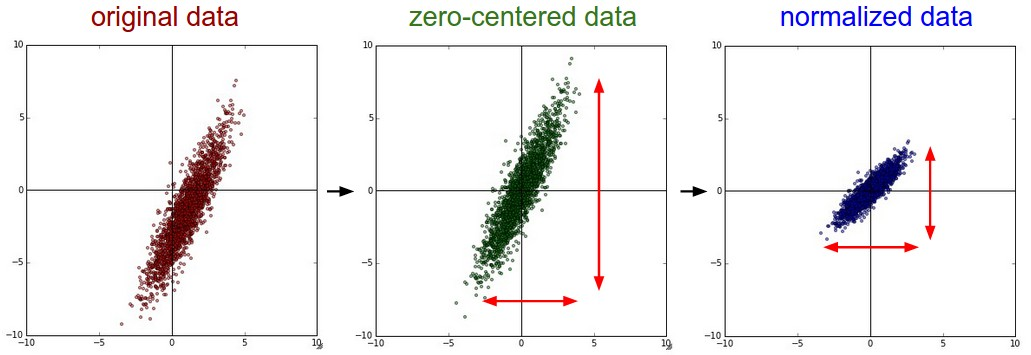
\includegraphics[width = 1.0\textwidth]{./Figures/normalization_1_prepro1.jpeg}
		\rule{35em}{0.5pt}
	\caption[Normalization]{Initialized weights of a neural network are usually randomly assigned between $-1$ and $1$. So on average a feature that has large values will contribute more to the weighted sum than another smaller scaled feature by virtue of having a greater product with the weighting. The arbitrary scaling of feature values should ideally not alter the results but it has been found to at best slow learning down, and at worst severely reduce model performance. Data will be normalized such that features are zero centred (centre graph), and the range of each feature made equivalent(right graph). By convention the range is between $-1$ and $1$}
	\label{fig:Normalization_2}
\end{figure}

\textit{Standardization} is another normalization method that not only rescales values over a similar range centered at the origin but to also have unit-variance as in Figure ~\ref{fig:Normalization_2}.
\be
x^\prime = \frac{x-\bar{x}}{\sigma}
\ee
where $\bar{x}$ is the mean of feature $x$ and $\sigma$ is the standard deviation.

In addition, feature variable may often be correlated.
This causes a problem for gradient descent, making optimization take longer\citep{featureScaling}.
Frequently a decorrelation method is used to transform the current set of features to a new set without correlation between variables.
Consider Figure ~\ref{fig:Normalization_3} where two features are strongly correlated with one another.
This can be treated simply with a linear transform to the feature vector which effectively rotates the axes to lie along the lines of correlated variables.
While most decorrelation algorithms are linear, non-linear decorrelation transforms do exist.
Decorrelation of features is often known as \textit{data whitening}
\begin{figure}[htbp]
	\centering
		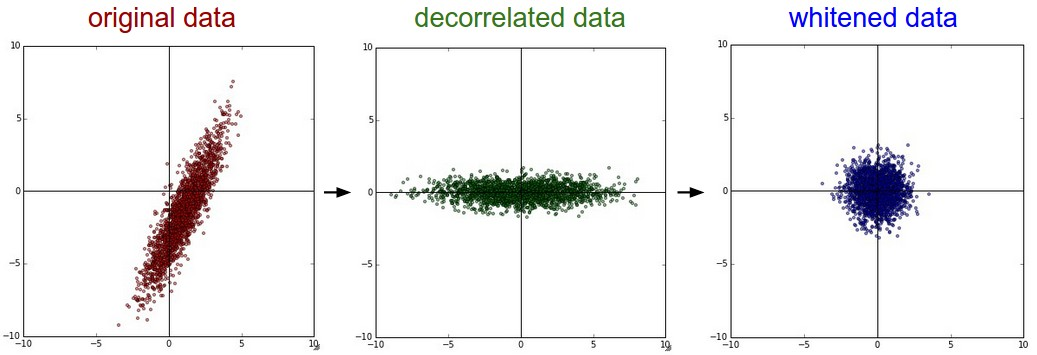
\includegraphics[width = 1.0\textwidth]{./Figures/normalization_2_prepro2.jpeg}
		\rule{35em}{0.5pt}
	\caption[Decorrelation]{Rescaling and centering data will still not be optimal for many machine learning algorithms. After zero centering, as in Figure \protect\ref{fig:Normalization_2}, there are still correlations in the data. That is, knowing the value of feature $x$ can inform you about the value of feature $y$. The slanted elliptical data distribution means the greater in value feature $x$ is, the more likely feature y will be larger. This is not ideal for learning because weightings on different features are now related which slows down the learning process and makes model interpretation more difficult. This issue can be dealt with by decorrelation. For linear correlations a rotation in feature space after zero-centering will work (center image). The features will still be on different scales. Decorrelation followed by rescaling the data (image on right) is known as \textit{data whitening}.}
	\label{fig:Normalization_3}
\end{figure}

%Batch Norm
So far we have spoken only of feature normalization, but neuron activations between layers may also be normalised in what is known as \textit{batch-normalization}.
Although inputs may be normalised, as the features are processed through the network, neuron activations may have gradually deviated from zero mean, unit-variance and become correlated in what is called \textit{co-variate shift}.
To correct for this Batch Normalization is often applied, which means for every batch of examples fed through the network a transformation is applied to the activations to keep the mean close to 0 and the standard deviation close to 1.
Batch Normalization ultimately results in faster, more accurate networks\citep{ioffe2015batch}.

\subsection{Learning Decay}
Throughout training, learning-rates tend to be either too small or too large for the local cost-surface.
Early in training a large step-size is desirable to quickly navigate down to a minima.
If the learning rate were to be smaller in these regions gradient descent can converge to the local minima.
Near the bottom a smaller step-size prevents over-shooting or oscillating over the minima.

Learning-decay tackles this by making the learning-rate, $\eta$, a function of the epoch number $i$
\be
\eta(i) = \eta_0 \frac{1}{(1 + \gamma i )}
\ee
where $\eta_0$ is the initial learning-rate and $\gamma$ is the decay constant.
Empirically learning decay has been shown to speed up learning and train more accurate models\citep{bengio2012practical}.
\begin{figure}[htbp]
	\centering
		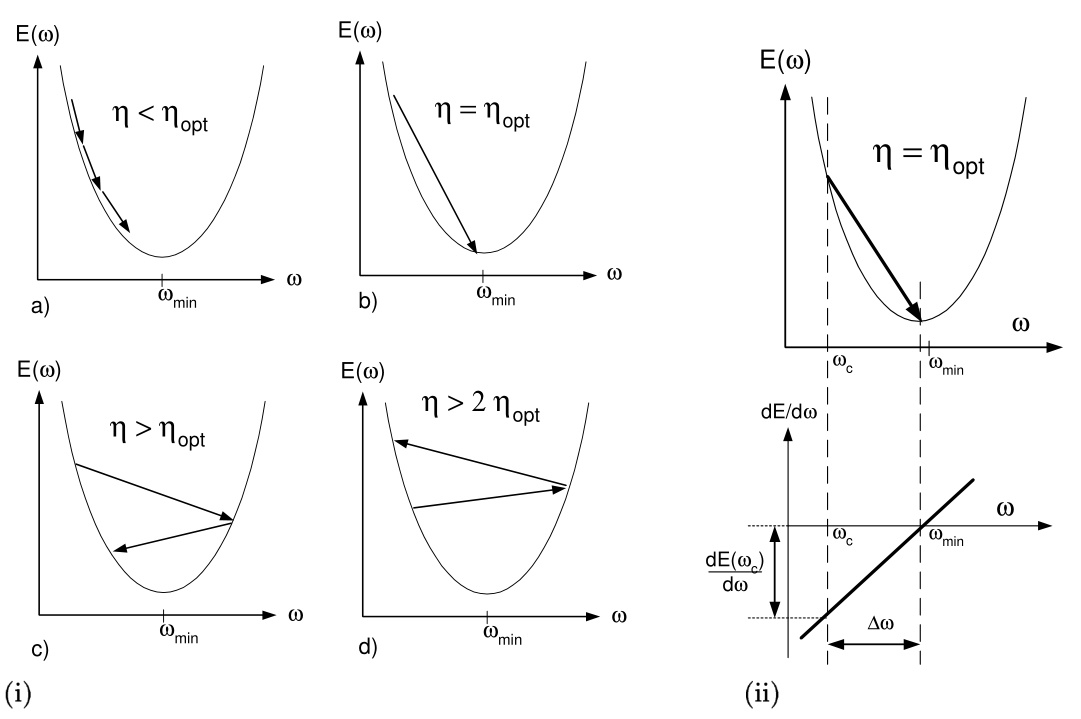
\includegraphics[width = 1.0\textwidth]{./Figures/efficient_backprop_learning_rate_issues.jpg}
		\rule{35em}{0.5pt}
	\caption[Optimum Learning Rates]{Where the gradient is negative the minima lies to the right, so adding the negative of the derivative multiplied by some constant $\eta$ will take the weight toward $\omega_{min}$. An optimal magnitude for $\eta$ will update the weight perfectly, as in (ii). This optimum value is usually not known ahead of time, so (i) explores the results of having a differing value. Where $\eta < \eta_{opt}$, see a), the weight updates will slowly approach the minima. Where $\eta$ is slightly larger than $\eta_{opt}$, see c), weight updates will oscillate over the minima. Too large a learning rate -  $\eta > 2\eta$ in the simplified case of a parabolic cost function - and the model weights will diverge.}
	\label{fig:Learning_rate_tuning}
\end{figure}


\subsection{Activation Functions}
Non-linear activation functions are used so as to be able to approximate non-linear relationships in the data\citep{bengio2009advances}.
A commonly used activation function is the sigmoid, shown in Figure ~\ref{fig:sigmoid}, which is given by the equation
\be
f(x) = \frac{1}{1 + e^{-x}}
\ee
and the hyperbolic tanh function\citep{bengio2009advances}.

Weights must be initialized such that activations are not saturated, especially in higher layers.
A saturated neuron is one that outputs a value near an activation function asymptote where the gradients are tiny.
should the neuron start, or become, saturated during training the back-propagated signal multiplied by the gradient will approach zero, effectively stopping the back-prolongation signal\citep{krizhevsky2012imagenet}.
\begin{figure}[htbp]
	\centering
		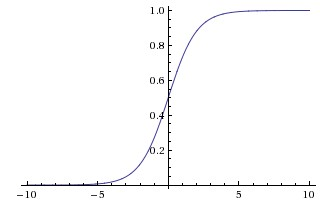
\includegraphics[width = 0.5\textwidth]{./Figures/sigmoid.jpeg}
		\rule{35em}{0.5pt}
	\caption[The sigmoid]{The ReLU funciton, $max(x,0)$, trains better performing networks significantly faster
	than the equivalent MLP using the $tanh$ or sigmoid activation functions.
	However where $x<0$ the neuron is \textit{dead}, or has a gradient of zero.}
	\label{fig:sigmoid}
\end{figure}


In theory, no non-linearity has more expressive power than any other, as long as they are continuous, bounded and monotonically increasing\citep{hornik1991approximation}.
However, the rectified linear unit (ReLU), shown in Figure ~\ref{fig:ReLU}, has been found to train faster\citep{nair2010rectified}.


Being a simple $max(0,x)$ operation, ReLUs quickly compute and are trained faster than both $sigmoidal$ and $tanh$ activations, see Figure ~\ref{fig:Relu_vs_sigmoidal} and Figure ~\ref{fig:Relu_vs_tanh}\citep{krizhevsky2012imagenet}.
In addition they do not require normalization to prevent saturation\citep{krizhevsky2012imagenet}.
If just a few examples produce a positive input to a ReLU, then learning will take place on that neuron.
However, ReLUs can die during training.
A dead ReLU is one in the $-\infty < x < 0$  region where the gradient is zero which prevents training of the neuron and layers below.
\begin{figure}[htbp]
	\centering
		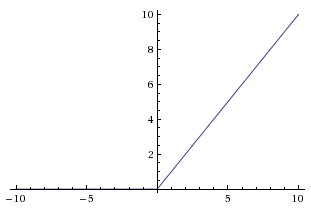
\includegraphics[width = 0.5\textwidth]{./Figures/relu.jpeg}
		\rule{35em}{0.5pt}
	\caption[The ReLU]{Of recent invent\citep{nair2010rectified} was the use of the ReLU activation function in MLPs. $g(z)_{ReLU} = max(0, z)$ has been found to train networks significantly faster which perform better than equivalent MLPs using sigmoidal activation functions..}
	\label{fig:ReLU}
\end{figure}
\begin{figure}[htbp]
	\centering
		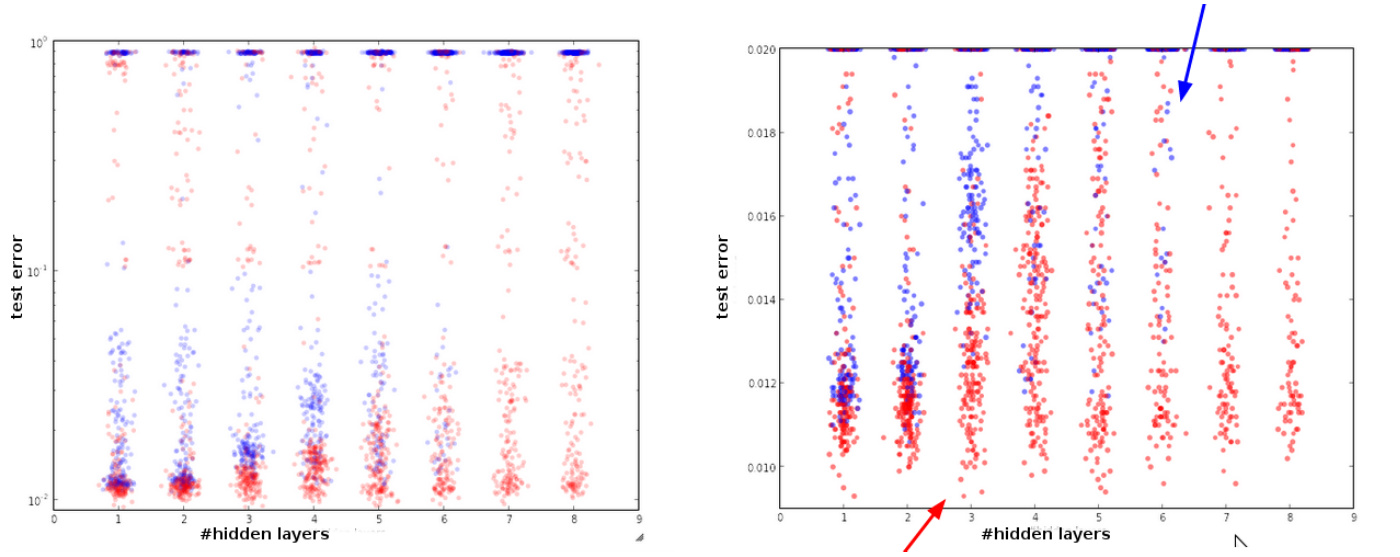
\includegraphics[width = 1.0\textwidth]{./Figures/effects_of_hyperpram_on_SGD_Bruel_relu_vs_sigmoidal.jpg}
		\rule{35em}{0.5pt}
	\caption[ReLU vs. Sigmoidal]{Models learned after being initialized with different weight parameters may differ in performance. One study\citep{nair2010rectified} explored the effects of using ReLU over the more traditional Sigmoidal activation functions. Many models of differing number of hidden layers and initialized weights were trained on the same data to see how activation functions affect performance. The graph on the left showing log(Test Error) vs. number of hidden layers shows a clear patter of ReLU models (in red) outperforming sigmoidal models (in blue) by two orders of magnitude at peak model performance densities. Zooming in on errors of order $10^{-2}$ on the right, the affect becomes more pronounced in larger models where ReLU models not only perform better on average but have error-rates no sigmoidal MLP ever achieves. }
	\label{fig:Relu_vs_sigmoidal}
\end{figure}
\begin{figure}[htbp]
	\centering
		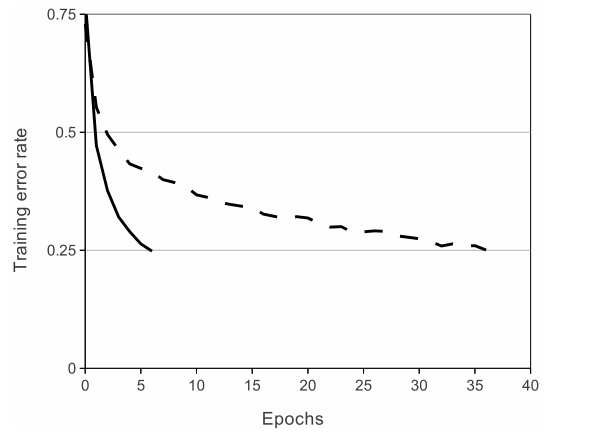
\includegraphics[width = 0.9\textwidth]{./Figures/Image_classification_with_DCNNS_relu_vs_tanh.jpg}
		\rule{35em}{0.5pt}
	\caption[ReLU vs tanh]{ReLU activation functions have been demonstrated to not only produce more accurate models but train significantly faster. Shown above the Training Error rate vs No. of Training Epochs. A four layer Neural Net achieves 25 \% training error rate on the popular image recognition CIFAR-10 data-set\citep{krizhevsky2009learning} six times faster than the equivalent network using $tanh(z)$ activation functions. Learning rates were optimized independently for each model so as to make training as fast as possible for that activation function. The magnitude of the effect will vary for different model architectures however models trained with ReLUs tend to consistently learn several times faster than their tanh or sigmoidal model equivalents. }
	\label{fig:Relu_vs_tanh}
\end{figure}



 \subsection{Weight Initialization}

Initial weight values have significant importance in training speed and accuracy\citep{lecun2012efficient}.
Weights cannot all be set the same value.
If all neurons where equally weighted they would produce the same output leading to the same gradients in back-propagation making training futile.
This is not true for biases which are generally set to $0$.
ReLU biases however are set to be a small positive value such as $0.01$ to ensure all ReLU activations are in the positive regime.

It has been discovered that output variance grows with the number of neuron inputs.
Training is more effective when the variance is normalized to $1$  with scaling by the $\sqrt{fan_{in}}$ (the number of inputs)\citep{neuralnetworkinitialization}.
\be
w = \frac{\Sigma(1,1)}{\sqrt{fan_{in}}}
\ee
where $fan_in$ is the number of inputs and $E$ is a Gaussian of mean $0$ and standard deviation $1$.

More recent analysis by Glorot et al\citep{glorot2010understanding} suggests weights should be sampled from the Gaussian $E(r,r)$
where $r = \sqrt{\frac{6}{fan_{in} + fan_{out}}}$ and $fan_{out}$ is the number of output neurons.

From a comparative study Larochelle et al. found that using the same neuron-count in each layer fares better than a decreasing or increasing neuron-count.
The first hidden layer cannot be too small else it cannot capture enough information from the input, but too many neurons risks over-fitting.
However. for most tasks an over complete first hidden layer works better than an under complete one.
A rule of thumb for the first hidden layer is $2n + 1$ where $n$ is the number of input features.

\subsection{GPU Speed Up}
%time-consuming 
%Parallizable
%CPU
%GPU
%Practical Implementations

%time-consuming 
When dealing with neural networks of many millions of parameters and tens of thousands of training samples the training process can take weeks.
Most of the training time is spent on matrix operations.
These are matrix-vector products, used in forward and back-propagation. and vector outer-products when calculating weight updates.

%Parallizable
Matrix-matrix multiplications can be done substantially faster than an equivalent sequence of matrix-vector products thanks to parallelism.
Firstly by smart caching mechanisms as implemented in the BLAS library, and thanks to parallelism\citep{wang2013augem}.
The speed-up is generally not in proportion to the number of cores used due to high data transfer and the associated latency\citep{ciresan2012multi}.
For small matrices the multi-core computations may take even longer than a single core because of this.
However, parallelism is more efficient with larger matrices.
Each neuron in a layer receives input as a weighted sum, or dot-product.
As such, neural networks are highly parallelizable by nature.
Entire training batches can be processed simultaneously.


In recent years GPU's decreased training times by some two-orders of magnitude compared to CPUs\citep{ciresan2012multi}.
The typical CUDA-capable\citep{cuda} GPU has several multi-processors(MP)\citep{chen2014big}; each of which contains several streaming multiprocessors (SMs) to form a building block.
Within each SM there are several stream processors (SP) that share control logic and global low-latency high bandwidth memory bank.
The high bandwidth comes at the cost of a small amount of RAM and lower clock speed.
GPU's typically have between 2-8Gb compared to up to a terabyte for a CPU.
Unfortunately information must be sent to the GPU by the CPU via the PCI-E connector which is slow and with large latency.
A GPU's architecture allows for thousand of threads, or processes, to run concurrently, shown in Figure ~\ref{fig:GPU_and_CPU}.
While CPUs are designed to handle general computing workloads, with units capable of processing high accuracy 64-bit floating point numbers, GPU's are less capable in the kinds of operations they can handle but can execute many at once making them excel at linear algebra and matrix multiplications.
\begin{figure}[htbp]
	\centering
		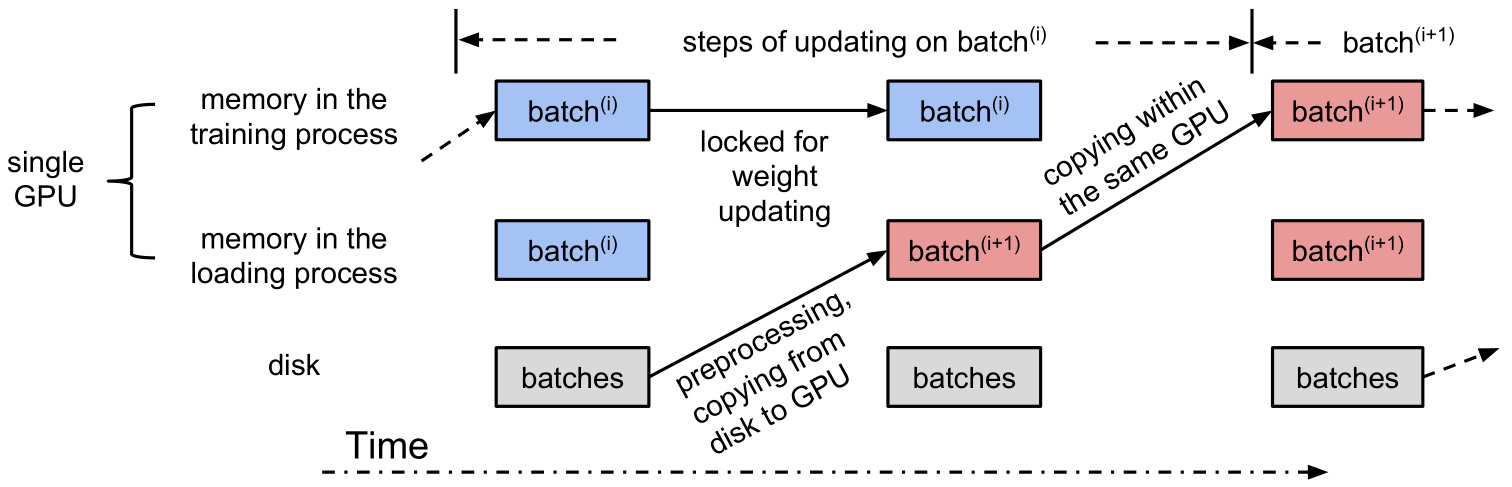
\includegraphics[width = 0.9\textwidth]{./Figures/Theano_based_large_scale_cisual_gpu_and_cpu_process.jpg}
		\rule{35em}{0.5pt}
	\caption[GPU Parallelized Training]{Graphics Processing Units (GPUs) excel at algebraic operations. GPUs were initially developed to use many cores for image-processing and the gaming industry. Despite each core being slower and with less allocated memory than a CPU, parallization allows for faster algebraic operations. Using a GPU, SGD on a GPU is handled like a production-line. Training batches are loaded onto the GPU (often pre-processed by the CPU). Then batches are simultaneously processed through the network to determine weight updates. Finally, model weights which are stored on the GPU are updated while the next training batch is loaded.
	\citep{neuralnetworkswebsite}}
	\label{fig:GPU_and_CPU}
\end{figure}


Unfortunately, programming GPUs is difficult, hard to optimize and requires specialized compilers.
Fortunately many software libraries, as in Figure ~\ref{fig:Theano}, have been developed at a higher level of abstraction to the GPU instructions.
For deep learning GPUs have become indispensable for model training in a reasonable time-frame. 
Together with libraries such as Theano and TensorFlow, models have been trained with over 100 million parameters.

\begin{figure}[htbp]
	\centering
		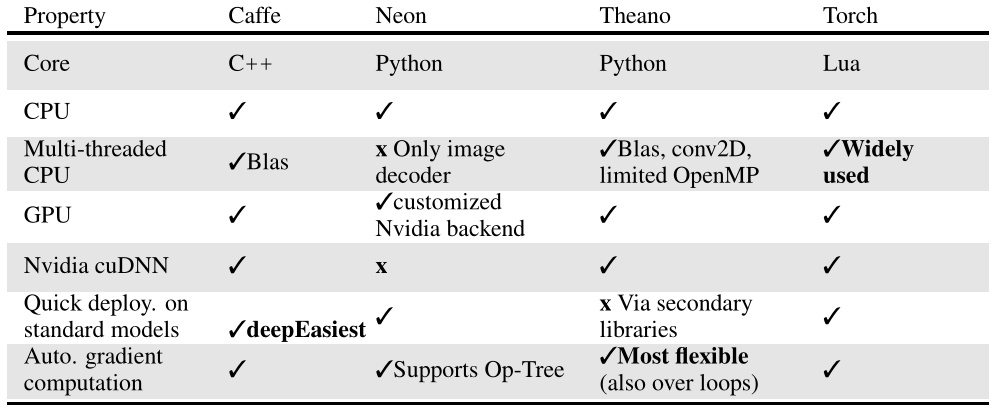
\includegraphics[width = 1.0\textwidth]{./Figures/theano_comparatives_study_of_cafe_neo_theano.jpg}
		\rule{35em}{0.5pt}
	\caption[Deep Learning Frameworks]{Several deep learning frameworks have been developed to accelerate model construction and training. Popular learning packages are shown above. The research in this thesis has been implemented using libraries built on top of the Python Theano framework. The open-source Theano, like several other frameworks, includes built in automatic gradient computation, commonly used functions, CPU multi-threading and GPU parallel processing on Nvidia hardware\citep{2016arXiv160502688short}.}
	\label{fig:Theano}
\end{figure}

  \section{Over/Under-fitting}
For a model to be useful it must generalize beyond the training data.
A model could have 100\% accuracy on the training data just by memorizing every example, but then it has not generalized at all. 
For an analogy; a student can learn to score 100\% on past paper questions if they appear in an exam but s/he has sacrificed general understanding for knowledge of particular questions and will likely perform poorly on unseen questions\citep{flach2012machine}.
S/he has \textit{over-fit} the training set of past papers but would not perform well on the test set (the exam), see Figure ~\ref{fig:Overfitting_2}.
\begin{figure}[htbp]
	\centering
		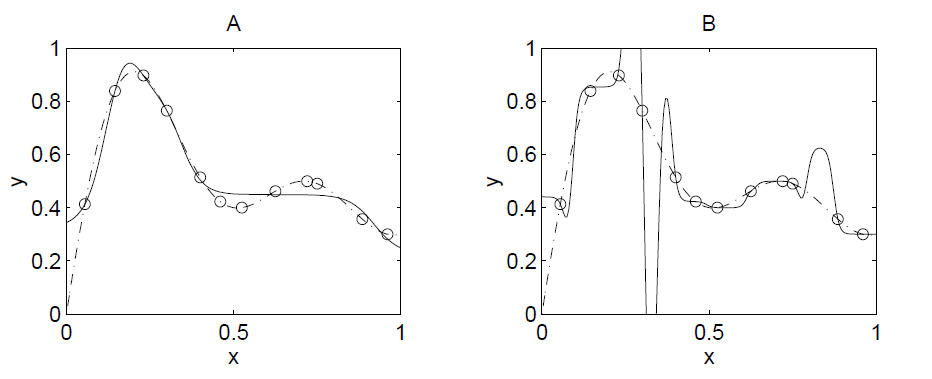
\includegraphics[width = 0.85\textwidth]{./Figures/An_intro_to_NNs_overfitting.jpg}
		\rule{35em}{0.5pt}
	\caption[Over-fitting]{A neural network is trained to predict $y$ from the $x$ feature based on the 12 examples, shown as circles. The dashed line shows the function from which the points were sampled. A) A network of 5 neurons in the hidden-layer is fitted to the data producing the function approximation shown by the solid line. The model fits well but appears to have some bias in the $0.4 < x < 0.9$ region where the model is insensitive to the variance within the training data. B) A network 20 hidden units is fitted. The significant number of parameters allows the model to fit perfectly, giving the correct prediction for every example feature. Bias is quite low in that the model is quite sensitive to variations within the data. However, variance is high as a small change in $x$ has extreme effects on the prediction. The model thus over-fits the training data and would not generalize to new data sampled from the original function.}
	\label{fig:Overfitting_2}
\end{figure}

This illustrates the need for splitting all the data into a \textit{training set} and \textit{test set}, illustrated by Figure ~\ref{fig:Training_and_Test}.
In order for this to work training and test samples must be representative of the underlying problem.
The test set must not be used in any way for training to remain an unbiased evaluation of the model's performance.
Should it be used for training, even indirectly, then the model can learn to fit the test set; like a student learning to pass a particular test and not have understanding of the subject.
This suggests that the model should not fully optimize performance on the training-set, see Figure ~\ref{fig:Peaking_effect}.
Over-fitting occurs more often in regression problems where the output is dependent on more than the information contained in the data set, such as environmental noise.
Should the model over-fit training data it is fitting to the noise and not the general trend.

\begin{figure}[htbp]
	\centering
		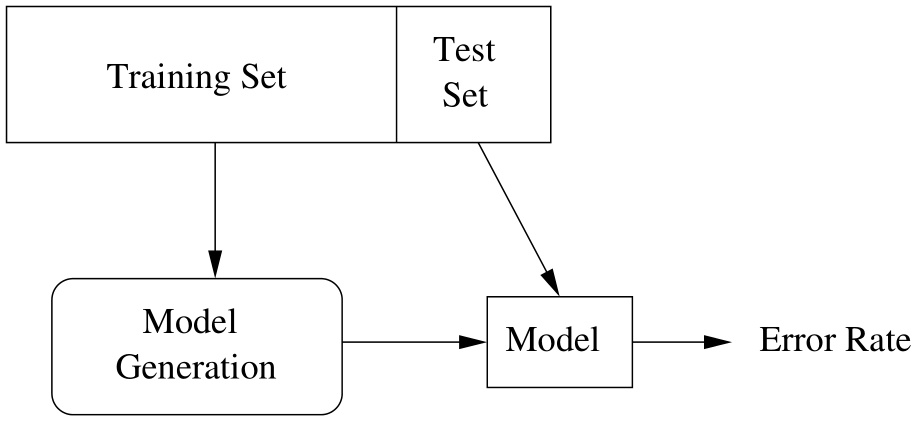
\includegraphics[width = 0.5\textwidth]{./Figures/training_and_test_sets_Mining.jpg}
		\rule{35em}{0.5pt}
	\caption[Model Training and Testing]{Model performance cannot be measured  with the training data as the result can be misleading. With enough degrees of freedom a model can fit the training data perfectly but generalize badly to unseen data. To avoid over-fitting the data is split into a training-set, and a test-set used only for an unbiased performance measure of the model.}
	\label{fig:Training_and_Test}
\end{figure}

\begin{figure}[htbp]
	\centering
		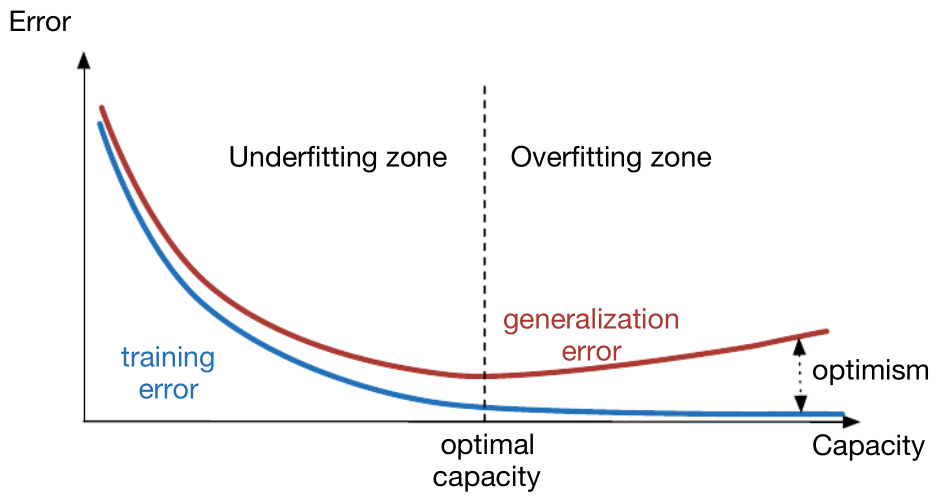
\includegraphics[width = 0.75\textwidth]{./Figures/overtraining_DL_textbook_6.jpg}
		\rule{35em}{0.5pt}
	\caption[Optimal Model Capacity]{The more parameters the more capacity (horizontal axis) a model has to fit training-data (bottom curve, blue) thereby reducing test error(top curve, red). Increasing capacity also expands the number of training samples a model can always fit. Training performance increases because the model fits the noise inherent to training data more than the general trend. Beyond the optimal capacity is the \textit{over-fitting regime}. Prior to the optimal model capacity, in the \textit{under-fitting regime}, there are not enough parameters to characterise the training data producing poor training and test performance results.}
	\label{fig:Peaking_effect}
\end{figure}

The `no free lunch' theorem formalized by Wolpert\citep{Wolpert96thelack} stipulates that no algorithm can beat random guessing over all possible functions to be learned seemingly supplanting machine learning altogether. 
However, real-world functions are not uniformly drawn from the set of all possible functions. 
Therefore it is reasonable to make assumptions that functions should be smooth, similar examples should have similar classes and simple functions are favoured over complex ones. 
Every algorithm must make assumptions beyond the data in order to generalize beyond the training data\citep{domingos2012few}.

Over and under-fitting can be described in term of \textit{bias} and \textit{variance}.
With too little complexity, loosely the number of parameters, a fitted model is \textit{biased}; insensitive to variation in the data.
For example a straight line fitted to points sampled from a sine function will not capture any of the oscillatory behaviour; the model has \textit{under-fit}.
In contrast, a highly complex function, as in the second frame of Figure ~\ref{fig:Overfitting_2}, can go through every point but introduces unnatural wiggles.
The model has high \textit{variance}; minor variations in the data would result in a very different model.
This illustrates the \textit{bias-variance dilemma}; too low complexity introduces systematic bias that no amount of data can resolve but too high and generalization is lost.

\subsection{Curse of Dimensionality}
Naively, intuitions formed in a 3D world suggest that the addition of features could only increase classifier performance.
However, with a large number of features potential benefit may be outweighed by the Curse of Dimensionality - a phrase coined by Bellman in 1961\citep{domingos2012few}.
Models generalize poorly in high dimensional data-sets for several reasons:

\begin{figure}[htbp]
	\centering
		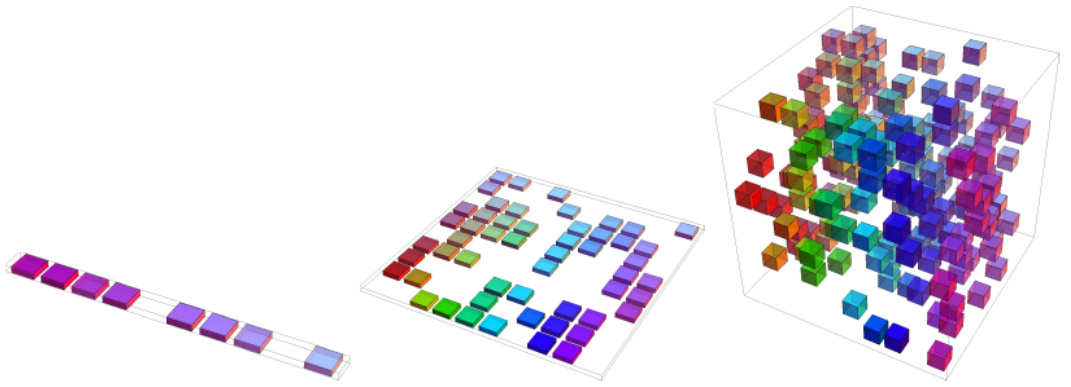
\includegraphics[width = 0.5\textwidth]{./Figures/Curse_of_dimentionality_DL_textbook_7.jpg}
		\rule{35em}{0.5pt}
	\caption[Curse of Dimensionality]{If 8 of 10 regions in a 1D feature space (leftmost image) are known; a density of 8/10 is sufficient to estimate values for the two unknown regions. In a 2D plane (center image) the number of regions grows to $10^2=100$. The number of samples needed to maintain the density is $0.8*10^2=80$. For a 3D feature-space (rightmost image) this escalates to 800 samples. In general the number of samples needed scales as $O(V^d)$ where $d$ is the number of dimensions and $V$ is the number of distinguishable regions per dimension.}
	\label{fig:Curse_of_dimensionality}
\end{figure}

\begin{enumerate}
\item When features are added to a fixed number of samples they cover a dwindling fraction of the feature-space.
If $n$ samples are required for an $R^1$ feature space to be considered dense, then $n^d$ samples are required to maintain the same density in $d$ dimensions, see Figure ~\ref{fig:Curse_of_dimensionality}.
The low data density in high dimensional space will require stronger and more accurate constraints\citep{cherkassky2007learning}.

\item Algorithms relying on similarity between samples (often a measure of the distance between points) break down.
Consider the K-nearest neighbour classifier. 
Unknown points are classified by comparing to the closest $K$ samples.
This is powerful in a densely packed low-dimensional space such as $R^2$.
However, with the addition of 98 irrelevant features ($R^100$), the irrelevant noise from the many features dominate the distance measure effectively making decisions random.

\item Even if all additional features are relevant, in a high dimensional space all examples can appear as nearest neighbours.
Consider the idealized case were examples are laid out on a regular grid.
In one dimension, the two nearest neighbours will lie on either side at the same distance from a sample $x_t$.
In two dimensions the four nearest neighbours lie at the corners of the square surrounding $x_t$. 
In general for a sample $x_t$ in $d$ dimensions the number of nearest neighbours is given by $2d$. 
In a high dimensional space so many samples can be considered nearest neighbours, effectively making the $K$ nearest neighbours random.


\item Objects in higher dimensional spaces have a larger amount of surface area for a given volume than objects in low dimensional spaces.
For example most of the volume of a multivariate Gaussian distribution comes not from near the mean (where the values are large) but much further out where the tails of the distribution are small but sweep into a much larger volume than near the core.
Put in another way, most of the volume of a higher dimensional orange comes not from the pulp but the thin sliver of skin far from the center.
it follows that in order to enclose even a small fraction of the data a large radius is required\citep{vladimir1998learning}.
The edge length of a unit-hypercube required to contain a fraction $p$ of the samples is given by 
\be
e_d(p) = p^{1/d}
\ee
where $d$ is the number of dimensions.
In order to enclose just 10 percent of the total data the edge length is $e_{10}(0.1) = 0.8$.
Therefore very large regions are required to capture a small amount the of the data making it difficult to provide a local estimate for high dimensional data.

\item Most samples will be closer to an edge that to any other sample.
For a scenario in which $n$ data points are uniformly distributed in a $d$ dimensional sphere of unit radius, the mean distance between the origin and the closest data point is
\be
D(d, n) = \left(1-\frac{1^{1/n}}{2}\right)^{1/d}
\ee
In a $200$ dimensional space with 200 data points this translates to a median distance of $D(10,200)\approx 0.57$.
The nearest point to the origin is over half the way from the origin to the radius, which is closer to the boundary of the data.
Most data points are outliers in their own projection.
This can be illustrated by the idea of standing at the end of a porcupine quill.
Every other quill will appear far away and clumped near the center.
This illustrates the difficulty in prediction of the label at a given point as any point will on average be closer to the edge than the training data point and so require extrapolation.

\end{enumerate}

There is some respite from the curse of dimensionality.
In general examples do not populate the feature space uniformly but are concentrated in a lower dimensional manifold.
For example k-nearest neighbours performs well for handwritten digit recognition though the feature space is large even for small images.
A $28\times 28$ pixel image equates to a feature space of $28^2 = 784$ dimensions, however the digits will only live in a much smaller sub-space of the full feature space.


\subsection{Data Augmentation}
Data Augmentation is using label-preserving transformations on already existing data to generate more 

Consider training a dogs and cats classifier.
If it so happens that many of the cats face toward the left the network may learn to only recognize those facing leftward facing cats and not 'realize' the class in not dependent on orientation.
To reduce over-fitting of this kind for images it is common practice to apply label-preserving transformations to already existing data to generate more. 
This is known as \textit{Data Augmentation}\citep{chatfield2014return} \citep{goyal2014object}\citep{krizhevsky2012imagenet}.
Using augmented data typically boosts performance by about 3 percent\citep{chatfield2015fly} even in large datasets, such as Galaxy Zoo\citep{lintott2008galaxy}\citep{goyal2014object}.
Commonly applied image transformations are skewing\citep{mo2012survey}, translation, reflection, brightness adjustment\citep{krizhevsky2012imagenet} and rotation\citep{chatfield2014return}.

The use of data augmentation does introduce a new problem.
If every image has many variations made the resulting dataset will be many times larger than the original.
Some datasets, such as ImageNet\citep{deng2012imagenet}, are already massive and it would be impractical to store all this data\citep{goyal2014object}.
This problem is treated by applying data augmentation on the fly while the original image is in memory, producing a temporary training batch before being discarded.
In many implementations image transformations are applied by the CPU while the GPU is training on the previous batch of images being even more economical with computing time.


\subsection{Regularization}
If the model has more parameters than necessary it will tend to over-fit the training data\citep{goyal2014object}.
\textit{Regularization} is a method of ensuring over-fitting does not occur even when the model is over-complex for the task.

\subsubsection{Weight Decay}
The idea behind \textit{weight decay}, also known as \textit{L2 regularization} is to add a \textit{regularization term} to the cost $C_0$ to obtain the modified cost $C$:
\be
C = C_0 + \frac{\lambda}{2n}\sum_\omega \omega^2
\label{eq:L2_cost}
\ee
where $\omega$ is the weights vector, $n$ the number of samples and $\lambda$ is a scaling constant.
All things being equal the network will now prefer to use small weights.

To see why this helps reduce over-fitting consider back-propagation with the modified cost function of Equation ~\ref{eq:L2_cost}.
The partial derivative used in back-propagation will be 
\be
\frac{\partial C}{\partial \omega} = \frac{\partial C_0}{\partial \omega} + \frac{\lambda}{n}\omega
\ee
and 
\be
\frac{\partial C}{\partial b} = \frac{\partial C_0}{\partial b} 
\ee
Substituting this into the weight update rules from Equation \ref{eq:updateEquation} we see
\be
b \rightarrow b - \eta \frac{C_0}{\partial b}
\ee
and 
\be
\omega \rightarrow \omega - \eta \frac{C_0}{\partial \omega} - \frac{\eta \lambda}{n}\omega = \left( 1 - \frac{\eta \lambda}{n}\right)\omega - \eta \frac{C_0}{\partial \omega}
\ee
The update rule for the biases is unchanged but the weights are rescaled by a factor of $1-\frac{\eta \lambda}{n}$ referred to as \textit{weight decay}.
This rescaling is what is refereed to as weight decay.
The first term favours few and small weights, however weight can still increase if it causes a decrease in the unregularized cost function\citep{bengio2012practical}.

In L1 regularization the added term is the sum of weight absolute values:
\be
C_0 + \frac{\lambda}{n}\sum_w |w|
\ee
Naturally this is similar to L2 in that the model prefers smaller and fewer weights.
To consider the difference between L1 and L2 regularization let us again consider the update rule with the modified cost function:
\be
\frac{\partial C}{\partial w} = \frac{\partial C_0}{\partial w} + \frac{\lambda}{n} sgn(w)
\ee
where $sgn(w)$ is the sign of $w$.
A small caveat is that the derivative $\partial C / \partial w$ is not defined when $w = 0$.
So in that case the standard update rule will be followed\citep{neuralnetworkswebsite}, equivalent to defining $sgn(0) = 0$.
The update rule is then
\be
w \rightarrow w - \frac{\eta \lambda}{n}sgn(w) - \eta \frac{\partial C_0}{\partial w}
\ee
Both L1 and L2 regularization shrink weights, however in L1 regularization weights are shrunk by a constant amount, whereas in L2 it is in proportion to $w$.
For a large weight the L1 regularization term $|w|$ is smaller than that of L2, and so the decay is less than for L2.
However when weights are small L1 will decay more than L2.
L1 therefore tends to result in a more sparse network; one with a small number of heavily weighted neurons with the rest close to zero.
Of course both types of regularization terms can be included in the model.
The linear combination of both L1 and L2 is termed an \textit{elastic net}.

\subsubsection{Drop-out}
\textit{Drop-out} is a powerful regularization method introduced by Hinton\citep{hinton2012improving} in 2012 which has been shown to work well for large neural nets.
\begin{figure}[htbp]
	\centering
		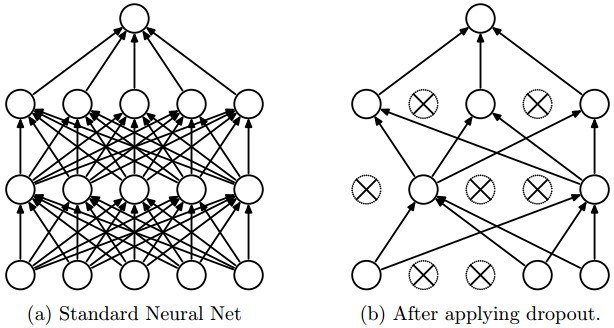
\includegraphics[width = 0.8\textwidth]{./Figures/dropout.jpeg}
		\rule{35em}{0.5pt}
	\caption[Drop-out]{Drop-out is an effective regularization method for MLPs. For every sample fed to the network only a fraction of randomly selected neurons may propagate the signal forward. This effectively creates a different architecture that shares weights with the original network. As a result neurons cannot rely on particular neurons from the layer below. This forces the network to generate a more robust representation of features from one layer to the next.}
	\label{fig:Dropout}
\end{figure}



In Drop-out a fraction $f$ of randomly selected neurons within a layer are prevented from propagating their signal to the layer above.
Neurons dropped out in this way contribute neither to forward-propagation nor back-propagation, as in Figure ~\ref{fig:Dropout}.
Instead of the layer computing $a=g(w.x)$ it now computes $a=m*\star g(w.x)$ where $m$ is a masking vector and $\star$ is the element-wise operator.
Activations of remaining neurons are multiplied by $1/f = 2$ to account for their being less active neurons\citep{goyal2014object}.
Now every time the input is injected, the neural network effectively samples from a different architecture sharing the same weights\citep{krizhevsky2012imagenet}.
As a result a neuron cannot rely on particular neurons firing from the layer below.
Instead individual neurons learn to detect more robust features, see Figure ~\ref{fig:Dropout_training}, which are helpful regardless of the large variety of internal contexts.

With Dropout the resulting model is the equivalent of training multiple networks and averaging their predictions.
Dropout may add up to a factor of two to training time but generates the equivalent of an ensemble in much less time\citep{krizhevsky2012imagenet}.

\begin{figure}[htbp]
	\centering
		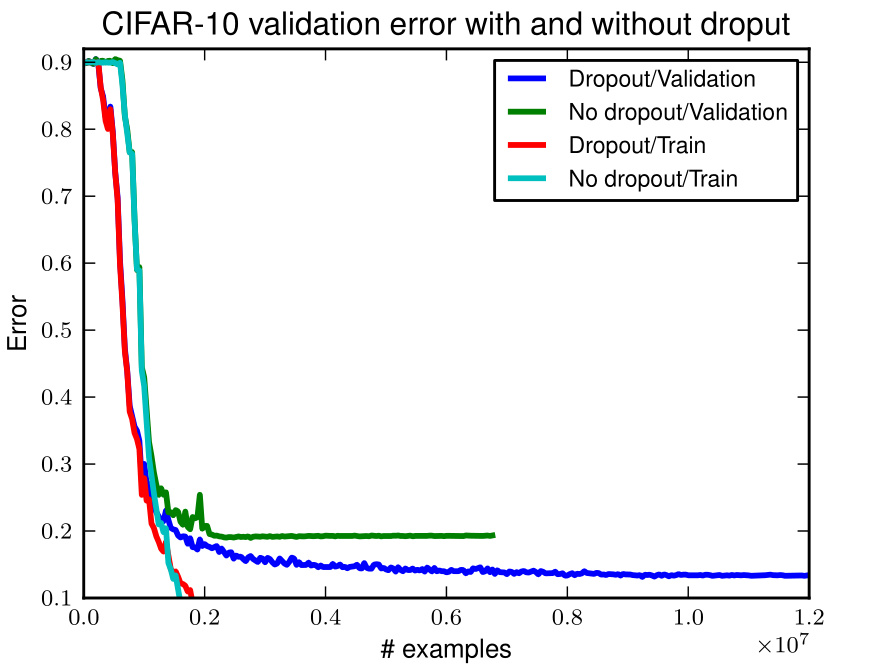
\includegraphics[width = 0.9\textwidth]{./Figures/training_with_dropout.jpg} %Dropout Benefits
		\rule{35em}{0.5pt}
	\caption[Drop-out Training]{A study\citep{wu2015towards} studied the effects of dropout on CNNs. Plotted above is model error vs the number of training samples. Error on the training set with drop-out (in red) is lower than without (in teal). The trend changes after $\approx 0.16\times 10^7$ training examples where the standard model over-fits the training set. Standard model validation error (in green) gets stuck in a local minima whereas the model with dropout (in blue) is continuously improving. This can be attributed to the changing network structure which alters the cost function and back-propagation signal. For few samples, < $1.6 \times 10^7$, performance is similar, however dropout helps prevent over-fitting.}
	\label{fig:Dropout_training}
\end{figure}

\subsubsection{Validation}
It is not enough to split the data into training and test sets to avoid over-fitting.
The practitioner could then tune model hyper-parameters by seeing which values lead to the best performance on the test set.
Doing this is indirectly training on the test data and no longer function as an independent source to evaluate the model\citep{witten2005data}.

This concern is what motivates the split of all the data into a training, validation and test set illustrated in Figure ~\ref{fig:Training_validation_and_Test}.
Typically the validation set is smaller than the training set so as to maximise training data.
Common practice is to split 70/30 for training and validation sets respectively.

\begin{figure}[htbp]
	\centering
		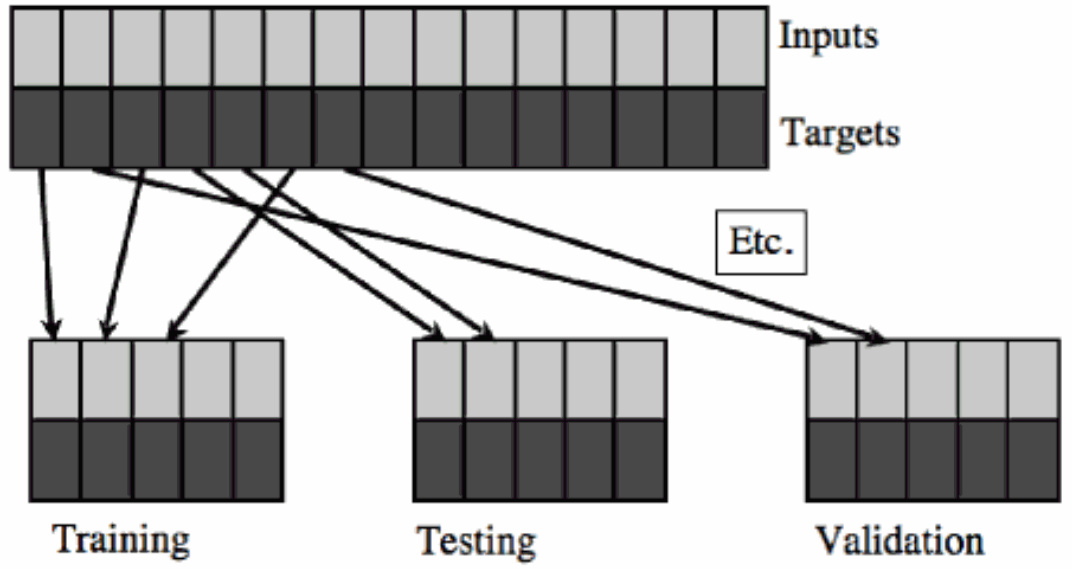
\includegraphics[width = 0.7\textwidth]{./Figures/training_validation_and_test_sets_ML_an_algorithmic_perspective.jpg}
		\rule{35em}{0.5pt}
	\caption[Validation]{If hyper-parameters are chosen based on test-set performance then the test-set is being indirectly fit to. This motivates splitting the data into three parts for training, validation and testing. The validation set is used for tuning hyper-parameters and the test set is used for measuring performance at the end.}
	\label{fig:Training_validation_and_Test}
\end{figure}

Hyper-parameters are tuned to maximise performance on the validation set and the completed model's performance is measured on the test set.\citep{barber2012bayesian}.

Once the hyper parameters have been selected and the model evaluated on the test set, it is possible to retrain the model on all the data.
With some well-behaved learning methods this is a reliable method to enhance the model\citep{witten2005data}.
However, to evaluate this new model a new source of test data must be created altogether.

\subsubsection{Cross Validation}
The more training data; the better the model. However, too little validation and test data makes for unreliable performance measures.
A commonly used method of K-fold cross-validation is used to handle the trade-off and is especially useful when there is little data altogether.

In K-fold cross validation the total data is split into $K$ equal sized partitions\citep{barber2012bayesian}.

See Figure ~\ref{fig:k_fold_validation_2} for an illustration of 5-fold cross validation.
\begin{figure}[htbp]
	\centering
		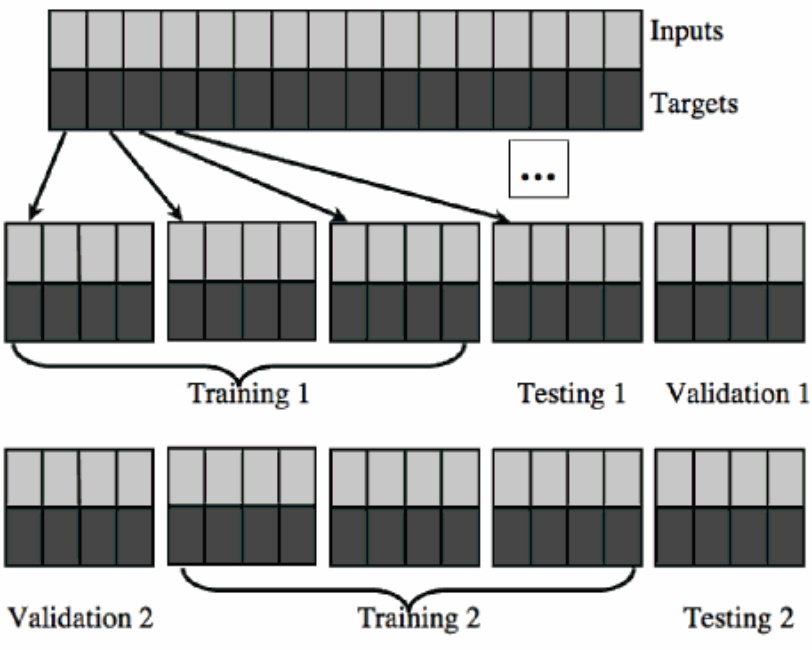
\includegraphics[width = 0.7\textwidth]{./Figures/ML_an_algorithmic_perspective_2_K_fold_validation.jpg}
		\rule{35em}{0.5pt}
	\caption[k-fold Validation]{For small datasets there may not be enough for training and validation sets. In K-fold cross validation the data is split in $K$ pieces to train $K$ different models each withholding a different piece for validation. The validation score is the average over all models.}
	\label{fig:k_fold_validation_2}
\end{figure}

The model is trained on the first $K-1$ partitions, leaving out the $K$'th partition as the validation set.
This is repeated for all $K$ combinations.
The validation performance is measured by taking the average performance of all $K$ models.
There is no objective rule what value to use for $K$. In practice it is common to use 10-fold validation.
An entirely unused test set must to used to measure the models final performance.

\subsubsection{Early Stopping}
%Early Stopping
If the model is over-complex it may over-fit if trained to convergence.
\textit{Early stopping}, see Figure ~\ref{fig:Overfitting_1}, is an inexpensive way to avoid over-fitting by stopping training ahead of convergence.
\begin{figure}[htbp]
	\centering
		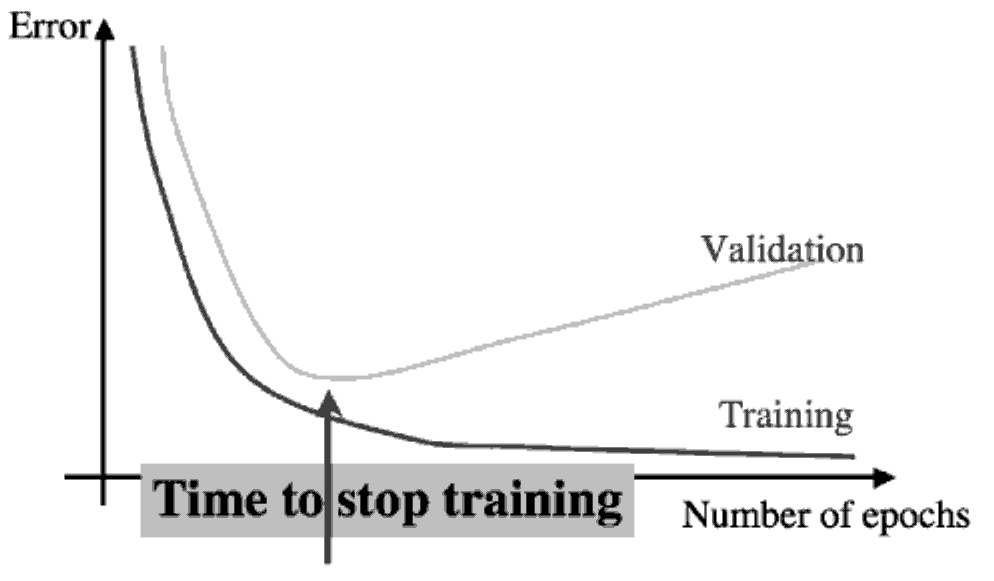
\includegraphics[width = 0.5\textwidth]{./Figures/machine_learning_an_aglorithmic_perspective_overfitting.jpg}
		\rule{35em}{0.5pt}
	\caption[Early Stopping]{\textit{Early-stopping} is a method of stopping training after a set amount of epochs to prevent over-fitting\citep{bengio2012practical}.}
	\label{fig:Overfitting_1}
\end{figure}

In one early stopping implementation the model is tested on the validation set after every $N$ updates.
Training is stopped when the model has performed best on the validation set\citep{bengio2012practical}.
Practically, training must go beyond the point of best validation error in order to detect the optimum epoch number.
Even if the model overshoots the optimum epoch-number, early-stopping will reduce over-fitting damage.
Unfortunately there is no a-priori  method to determine when to stop.
Instead, a few heuristics exist.
The one used in this thesis uses patience, which is the minimum number of training epoch before validation scoring which saves time in early training stages.
Once the threshold has been reached the validation score will be recorded after a further $N$ updates.
Should the new validation score be better than the previous training will continue for another $N$ updates otherwise training is halted.\citep{bergstra2010theano}\citep{bastien2012theano}.

\section{Deep Learning}\label{sec:deep_learning}
Machine learning methods typically use shallow-structured architectures.
These techniques have only one layer of non-linear feature transformations such as an ANN\citep{dengthree}.
Shallow architectures have proven to be successful in solving many simple or well-constrained problems, however their limited modelling and representational power is often insufficient for various real-world problems.
For example, image recognition\citep{dengthree} problems require the model to be insensitive to irrelevant variations, see Figure ~\ref{fig:Image_challenges}, such as lighting conditions, translations, rotations, pose, scale conformation and obstructions\citep{liu2014deep} while being sensitive to relevant variations such as distinguishing features of dog breeds.
A linear classifier would likely classify two different breeds of dogs as the same if they are in the same position and background.
Similarly a single breed of dog could be classified differently when in differing image contexts.

As a result shallow classifiers require smart feature extraction that solves the \textit{selectivity-invariance dilemma}; features must be selective of important variations and invariant to irrelevant ones.
Constructed features tend to be case-specific and require deep knowledge of the problem and data\citep{bengio2009advances}.
Depending on initial model performance features would then be redesigned in an iterative and time-consuming process, see Figure ~\ref{fig:deep_vs_classic_ml}.
\begin{figure}[htbp]
	\centering
		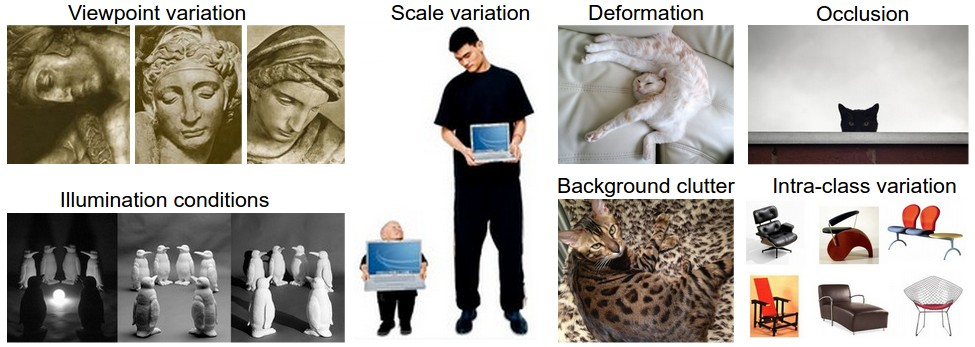
\includegraphics[width = 1.0\textwidth]{./Figures/challenges.jpeg}
		\rule{35em}{0.5pt}
	\caption[Image Recognition]{Image recognition is a difficult task as the very same object can appear with many irrelevant variations. For a model to be successful it must be impervious to these changes. For example, an object may vary in orientation(top left), lighting (bottom left), scale(middle) and distortion(one left of top right). In addition there may be contextual changes such as background clutter (one left of bottom right) and occlusion (top right). In addition the object class may vary in structure and colouring (bottom right) and yet still belong to the same class.}
	\label{fig:Image_challenges}
\end{figure}

\begin{figure}[htbp]
	\centering
		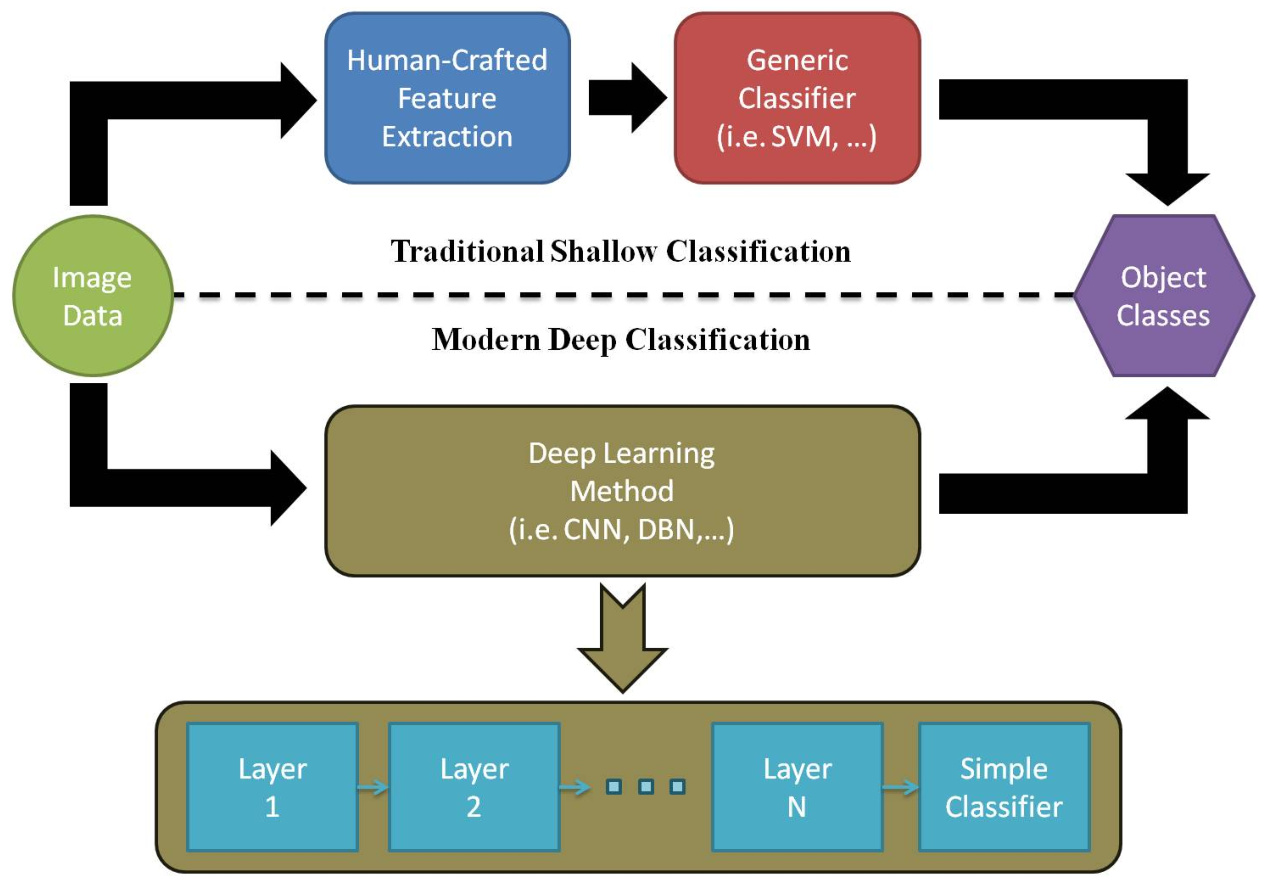
\includegraphics[width = 0.8\textwidth]{./Figures/deep_vs_classic_machine_leanring_sparse_coral_classification.jpg}
		\rule{35em}{0.5pt}
	\caption[Shallow vs. Deep Learning]{In shallow architectures features are manually created based on human analysis of the problem. Crafted features are then fed to one of many possible classifiers and tuned for peak performance. In contrast, no human-crafted features are necessary in deep-learning. Instead, the multi-layered architecture will learn the appropriate feature transformations to construct the most useful features. The final layer of the network presents these learned features to a simple classifier.}
	\label{fig:deep_vs_classic_ml}
\end{figure}

Speech exhibits hierarchical layered structure from the waveform level of sound to a linguistic level of speech\citep{baker2009variability}.
Similarly the visual systems are also hierarchical in nature.
Pixels may be assembled into edge-lets, edge-lets to motifs, motifs to parts, parts to objects, and finally objects to scenes\citep{lecun2010convolutional}.
This suggests that machine learning methods adopt hierarchical structure.
A \textit{deep-learning} architecture is a multilayer stack of simple modules which compute non-linear input-output mappings.
Each module in the stack performs a transformation on the input to increase selectivity and invariance of the feature-set.
See Figure ~\ref{fig:learning_complex_features} for an example of a multi-layered architecture developing better feature representations at every layer for facial recognition.
A deep architecture can eliminate feature extraction altogether\citep{lecun1995convolutional}.
The first few layers learn features directly from the input data, illustrated in Figure ~\ref{fig:first_layer_features}.
\begin{figure}[htbp]
	\centering
		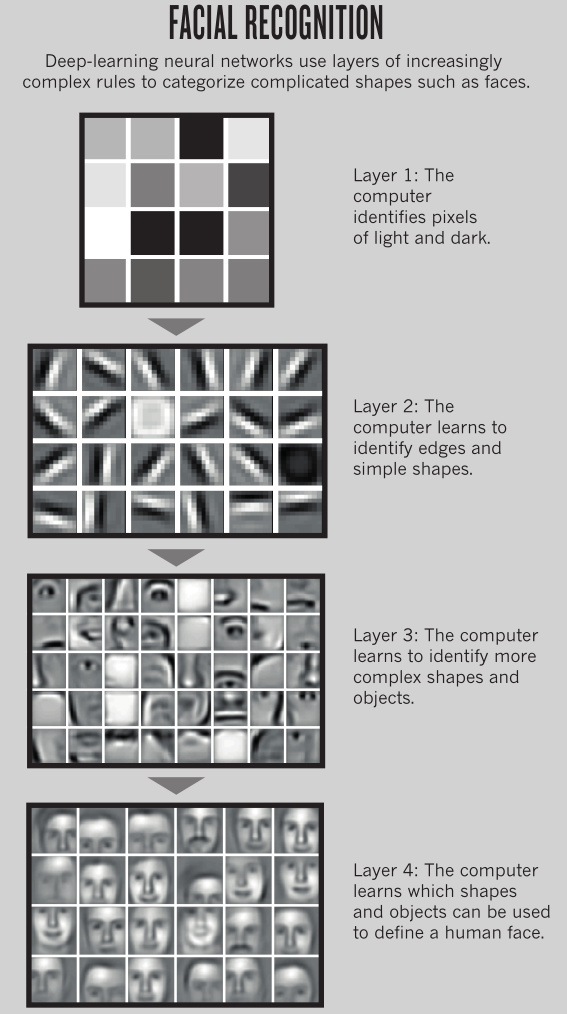
\includegraphics[width = 0.7\textwidth]{./Figures/learning_complex_features_the_learning_machine_nature.jpg}
		\rule{35em}{0.5pt}
	\caption[Learning Complex Features]{Deep Learning utilizes a multi-layered architecture to construct complex features of the input data. A model for facial recognition takes in pixel values as input. Layer 1 identifies light and dark pixels. Layer 2 learns to identify edges with different orientations and simple shapes from the output features of Layer 1. Layer 3 identifies more complex shapes and features from simpler shapes and edges. Layer 4 learns which complex shapes and objects define a human face. A face's image decomposed into its different parts and shapes can then be used to identify the person.}
	\label{fig:learning_complex_features}
\end{figure}
\begin{figure}[htbp]
	\centering
		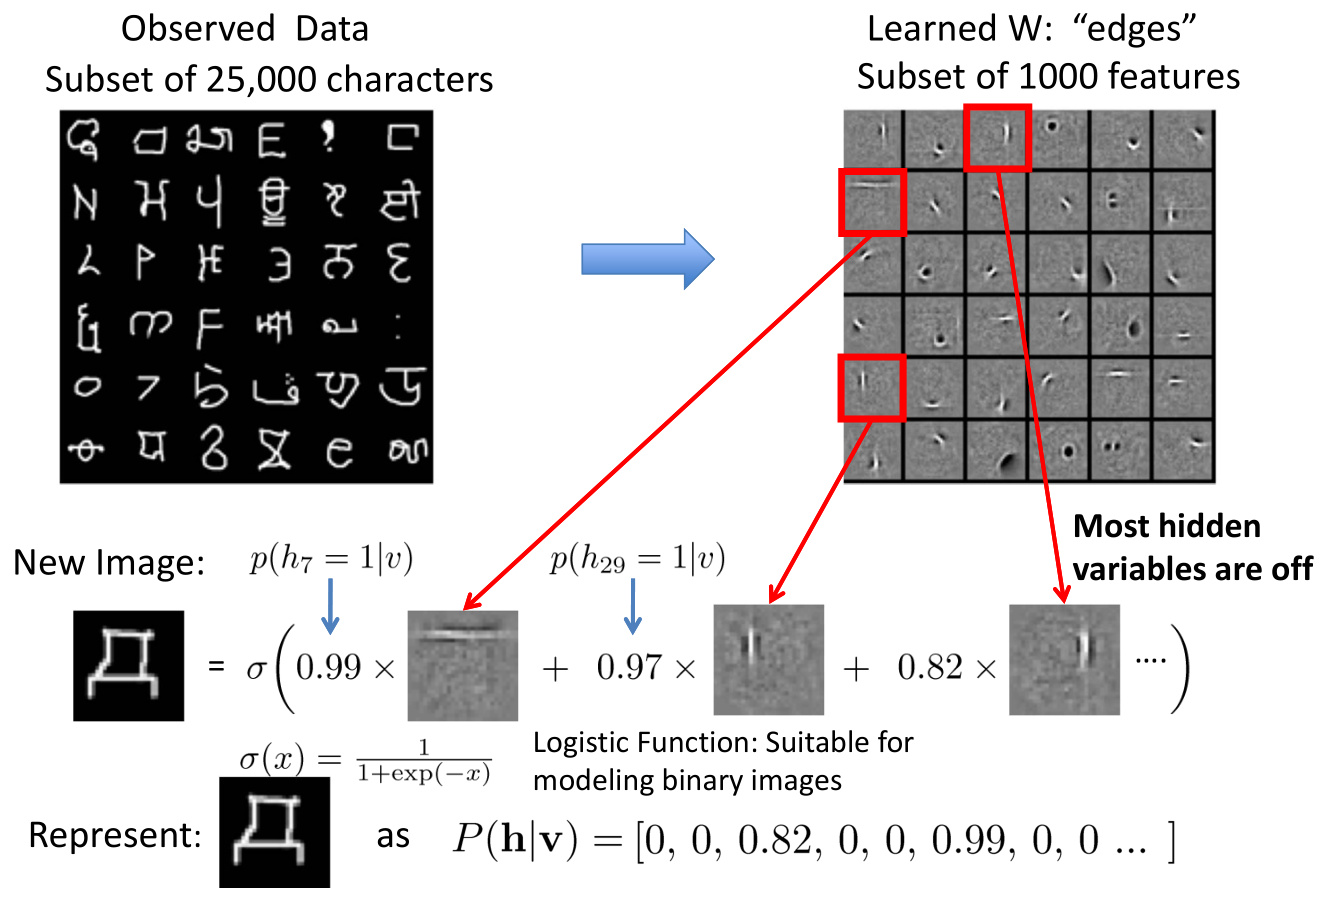
\includegraphics[width = 0.85\textwidth]{./Figures/Deep_Learning_Russ_Salakhutdinov_first_layer_features.jpg} %First layer visualization
		\rule{35em}{0.5pt}
	\caption[Learned Features]{Samples characters from a 25, 000 character dataset are shown above\citep{salakhutdinov2009deep}. Designing features that best capture information relating to these characters would take plenty work and insight. Deep Learning can learn complex features directly from the data. On the right we can see a sample of what image characteristics provide the most activation to neurons higher up in the network. The network has learned to use edge detectors at different locations and orientations. Now a character can be decomposed into 1000 coefficients of the feature maps rather than manual feature construction.}
	\label{fig:first_layer_features}
\end{figure}

\textit{Deep Learning} (DL) algorithms are inspired by the human brain\citep{mo2012survey}\citep{chen2014big}.
The brain quickly processes complex data, learns in different domains and solves complicated tasks.
DL aims to deal with high-dimensional data efficiently and quickly; performing complicated tasks such as image and sound recognition.
As Bengio and Lecun put it, ``Deep architectures are compositions of many layers of adaptive non-linear components, in other words, they are cascades of parametrized non-linear modules that contain trainable parameters at all levels''\citep{bengio2007scaling}.
DL refers to supervised or unsupervised algorithms with many layers of information processing that learn hierarchical representations of the data\citep{chen2014big}\citep{dengthree}.
While there were multiple deep architectures before 2006, almost none were successful is terms of accuracy and efficiency with the exception of Convolutional Neural Networks (CNNs)\citep{lecun1995convolutional}. 

DL methods have had many successful applications.
Visual document analysis\citep{simard2003best}\citep{karnowski2010deep}, facial\citep{le2013building}\citep{farfade2015multi} and speech recognition, natural language processing, human action recognition\citep{ji20133d}\citep{mo2012survey}, facial location \citep{liu2014deep}, image semantic discovery\citep{liu2014deep}, image compression\citep{goyal2014object}, collaborative filtering\citep{chen2014big}, and Medical Diagnosis\citep{goyal2014object}.
Companies such as Google, IBM, Apple and Facebook have all been aggressively pursuing DL projects.
Google has used DL for voice recognition, Street View and image recognition; Microsoft for their real-time language translation in Bing voice search\citep{dahl2011large}, and IBM for their Jeopardy winning Watson\citep{ferrucci2013watson}\citep{chen2014big}.
Siri, the iOS assistant, gives weather reports, provides news, answers questions and gives reminders all with the power of DL\citep{chen2014big}.
The recent enthusiasm for DL is largely a result of increased hardware capabilities, specifically GPUs, cheaper computing equipment and recent advances in research\citep{dengthree}.
As Big Data only gets bigger, DL will play a larger role in predictive analytics especially considering the advances in computing power and use of parallel processing in GPUs\citep{chen2014big}.

Bengio and Lecun proposed the following requirements for a successful DL implementation\citep{bengio2007scaling} \citep{bengio2009learning}\citep{chen2014big}.
The algorithm must:

\begin{enumerate}
\item function with a large range of architectures.
\item handle deep architectures, and manipulate intermediate features with many levels of non-linear transformations.
\item sample from a large space of possible functions with many millions of parameters.
\item scale efficiently with the number of parameters and samples. This prohibits algorithms that iterate many times over the data.
\item discover multi-use concepts(multi-task learning) and may use unlabelled data.
\end{enumerate}

\subsection{Convolutional Neural Networks}

\subsubsection{Introduction}

The Universal Approximation theorem by Hornik\citep{hornik1991approximation} states that a neural network with a single hidden layer can model any continuous function.
However, Bengio\citep{bengio2009learning} showed that a shallow network would require an exponentially large number of neurons when compared to a Deep Neural Network(DNN) with many hidden layers.
Recently in 2014, Romero\citep{romero2014fitnets} and Ba and Caruana\citep{ba2014deep} showed that a deeper neural network can be trained to perform much better than a comparatively shallow one.
However, DNNs typically require huge computational resources that make their training and real-time application difficult to implement\citep{goyal2014object},

DNNs face several challenges\citep{mo2012survey}:
\begin{enumerate}
\item DNN's cannot train on unlabelled data, which greatly outnumbers labelled data.
\item Back-propagation correction signals get severely weakened travelling through the neural network.
This results in layers near the top being altered, but layers near the bottom are largely unaffected; the \textit{gradient dilution problem}\citep{bengio2009learning}.
\item Learning is very slow for networks of many layers due to the many millions of weighted sums, activations and back-propagation signals that need to be computed.
\item The network is likely to end up in a poor local minima rather than the global one.
The severity of poor local minima increases significantly as network depth increases\citep{dengthree}.
\item The main deficiency of unstructured nets is their lack of built-in invariance with respect to translations and distortions\citep{lecun1995convolutional}.
For example, digits may appear with differing slants, sizes and positions.
Words are spoken with varying pitch, speed and intonation.
In principle, a sufficiently large network can learn to be invariant to such transformations, however that will likely result in multiple units with identical weight patterns and the number of training instances required is very large\citep{lecun1995convolutional}.
\item Due to the input data being vectorised and fed to the first layer, the topology of the input is ignored.
This is contrary to the fact that spectral representation of speech and images have strong local 2D structures and times series strong 1D local structure.
For example, pixels that are spatially or temporally nearby are highly correlated\citep{lecun1995convolutional}.
\item The large number of trainable parameters allows for easy over-fitting.
\end{enumerate}

In 1962 Hubel and Wiesels' revealed from studies of cats' primary visual cortex\citep{lecun1995convolutional}\citep{bengio2009advances}\citep{goyal2014object} that there is a hierarchy operating within neurons of the visual cortex in living organisms.
Simple neurons in the up-most layer connect to a small region of complex neurons below\citep{gabor1946theory}.
The first neural nets based on this insight were Fukushima's Neocognition and Lecun's Net-3\citep{bengio2009advances}.
In such an architecture the lower layer is divided into a smaller number of regions called \textit{Receptive Fields}, each of which is mapped to a single of the layer above\citep{bengio2009advances}.
The connection is called a \textit{feature extractor}.
Many such feature extractors are applied to the same receptive field generating a corresponding feature vector.

Advantages for this architecture include\citep{lecun2015deep}:
\begin{enumerate}
\item Sparse Connectivity - Rather than connect an entire layer to the layer above, each receptive field is connected to a single neuron, see Figure ~\ref{fig:sparse_vs_fully_connected}.
This significantly reduces the number of parameters which makes training much easier\citep{bengio2009advances} and faster.
Trials have consistently shown, see Figure ~\ref{fig:Sparsity}, that sparsely connected networks outperform their fully connected versions.
\item Shared weights - This means each receptive field is connected to the upper layer by an identical set of weights\citep{krizhevsky2012imagenet}\citep{lecun1995convolutional}, see Figure ~\ref{fig:parameter_sharing}.
Elementary feature detectors useful in one part of the image are likely to be useful everywhere\citep{lecun1995convolutional}.
This is a strong, yet justified, assumption in the locality of pixel dependencies.
This again significantly reduces the number of parameters that need to be learned improving training\citep{mo2012survey}\citep{bengio2009advances} and model generalization while the best possible theoretical performance is only slightly worse than for a fully connected DNN\citep{krizhevsky2012imagenet}\citep{lecun1995convolutional}.
\item Sub-sampling - Between layers input data is sub-sampled in what is known as \textit{pooling} which significantly reduces the number of parameters and computations required\citep{bengio2009advances}\citep{chen2014big}\citep{ciresan2012multi}.
\item Deep Architecture  - The many layered architecture allows for extracting highly non-linear and robust features.
\end{enumerate}
\begin{figure}[htbp]
	\centering
		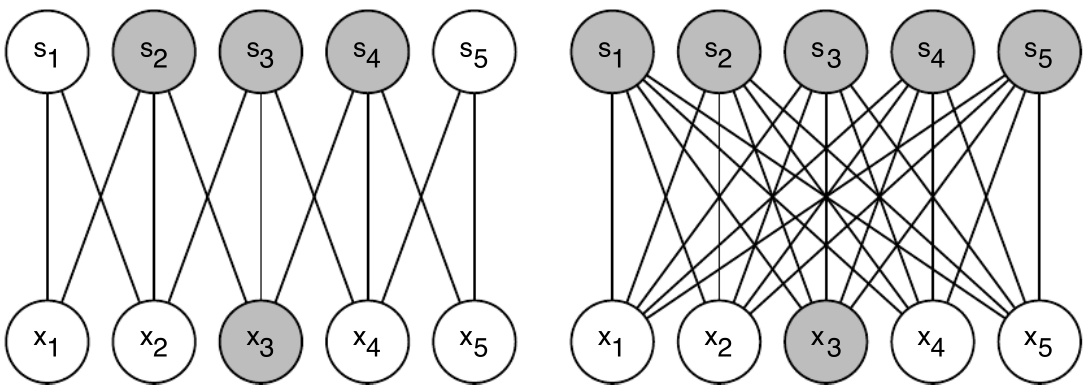
\includegraphics[width = 0.5\textwidth]{./Figures/Spars_verse_fully_connected_DL_textbook.jpg} %Sparse Connections
		\rule{35em}{0.5pt}
	\caption[Sparse Connectivity]{MLPs with full-connectivity between layers $L_1$ and $L_2$ have $N_1 \star N_2$ parameters, where $N_i$ is the number of neurons in layer $i$. For two layers of 5 neurons each there will be $ 5 \times 5 = 25$ connections. However, if neurons in $L_2$ may only connect to a local subset of neurons there is a significant reduction in the number of parameters $ 3 \times 3 + 2 \times 2 = 13 $ connections.}
	\label{fig:sparse_vs_fully_connected}
\end{figure}
\begin{figure}[htbp]
	\centering
		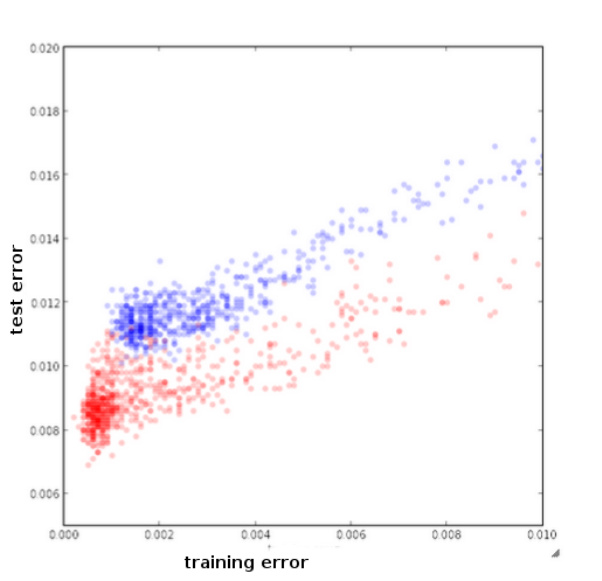
\includegraphics[width = 1.0\textwidth]{./Figures/effects_of_hyperpram_on_SGD_Bruel_CNN_Sparsity.jpg} %CNN vs Fully connected
		\rule{35em}{0.5pt}
	\caption[CNN vs. Fully Connected]{Naively on would think a fully connected network should outperform a CNN. However, the sparse and shared connections ensure back-propagation signals do not disappear and improves invariance to label-preserving transformations. The scatter plot depicts converged model performance on test and training sets for both CNNs (in red) and MLPs (in blue). Points to the bottom left are preferable as they have both low training and test errors. CNNs consistently outperform their fully connected counterparts in both test and training error for the majority of random parameter initializations.}
	\label{fig:Sparsity}
\end{figure}
\begin{figure}[htbp]
		\centering
			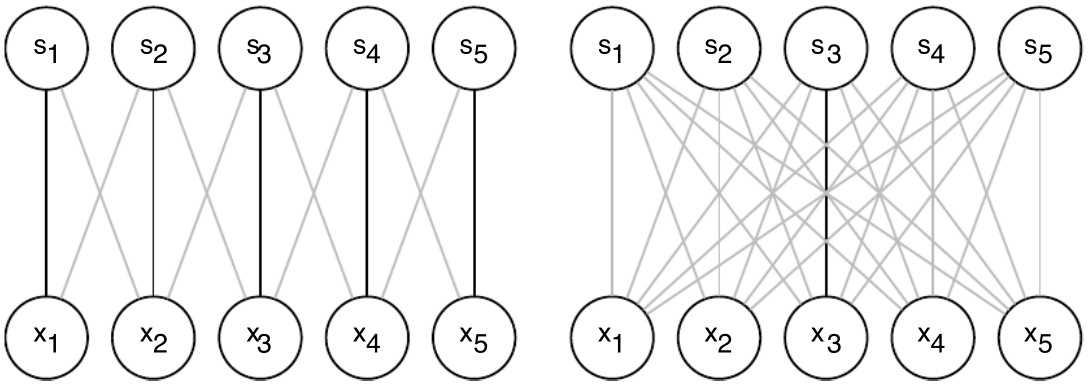
\includegraphics[width = 0.9\textwidth]{./Figures/parameter_sharing_DL_textbook_2.jpg} %parameter sharing
			\rule{35em}{0.5pt}
		\caption[Parameter Sharing]{The network on the left makes use of parameter-sharing; bold lines show all the connections equal to the $x_3$ to $s_3$ weight. In total there are three unique weights. In contrast, the fully-connected network on the right has $5^2 = 25$ unique weights.}
		\label{fig:parameter_sharing}
\end{figure}

The resulting model, a \textit{Convolutional Neural Network}(CNN)\citep{dengthree}, learns hierarchical representations of the data using local receptive fields, shared weights and sub-sampling and is more resilient to variations within the data\citep{lecun2010convolutional}.

A typical CNN is composed of many layers; some for feature representations, known as \textit{feature maps}, and others as conventional neural networks.
The input and output of each stage is a set of matrices called feature maps.
In the case of a colour image, the input to the first layer can be thought of as an input of three feature maps; each a 2D array containing a colour channel of the image.
For audio input this is a 1D feature map, for video or a volumetric image (such as an MRI) the feature maps are 3D.
Each feature map represents a particular feature at all locations over the image, such as vertical lines.
A CNN alternates between two types of layers, \textit{convolutional} and \textit{pooling}, which together make up a single CNN stage\citep{chen2014big}.
There will be several such stages followed by a set of fully connected neurons to form a classification module\citep{lecun2010convolutional}.

CNNs have been successfully used in many commercial projects including Optical Character Recognition, handwriting recognition (including Arabic and Chinese),video surveillance\citep{bengio2009advances} and speech recognition\citep{dengthree}\citep{haffner1998high}\citep{krizhevsky2012imagenet}\citep{donahue2014decaf}\citep{simonyan2014very}\citep{abdel2012applying}\citep{sainath2013learning}.
The first commercial deployment was for check reading ATM machines in Europe in 1993\citep{bengio2009advances}.

\subsubsection{Convolution}
Each convolutional layer constructs several feature maps convolving input with different feature filters (weight matrices).
The value of each pixel in the feature map is the result of connecting a small defined region of the input below to a single neuron above, refer to Figure ~\ref{fig:CNN_2}.
Weights used in this connection are the filter which will move over the whole image to generate different pixels in the above feature map.
The application of several different filters will produce the same number of feature maps\citep{lecun2010convolutional}\citep{mo2012survey}.
Expressed as a vector equation with pixel location indices suppressed,
\be
y_j^{(l)} = f\left(\sum_i K_{ij} \otimes x_i^{(l - 1)} + b_j \right)
\ee
where $Y_j^{(l)}$ is the $j$-th feature map of the $l$-th convolution layer, and $f$ is a non-linear activation function\citep{lecun2010convolutional}\citep{mo2012survey}\citep{chen2014big}.
$K_{ij}$ is a trainable filter (or \textit{kernel}) that convolves with feature map $x_i^{(l - 1)}$ from the previous layer to produce a new feature map in the current layer as illustrated in Figure ~\ref{fig:Convolution}.
Symbol $\otimes$ is the discrete convolution operator and $b_j$ the bias term.
Each filter $K_{ij}$ can connect to all or a portion of the feature maps from the previous layer.
The weights $K_ij$ are trained via back propagation.

\begin{figure}[htbp]
	\centering
		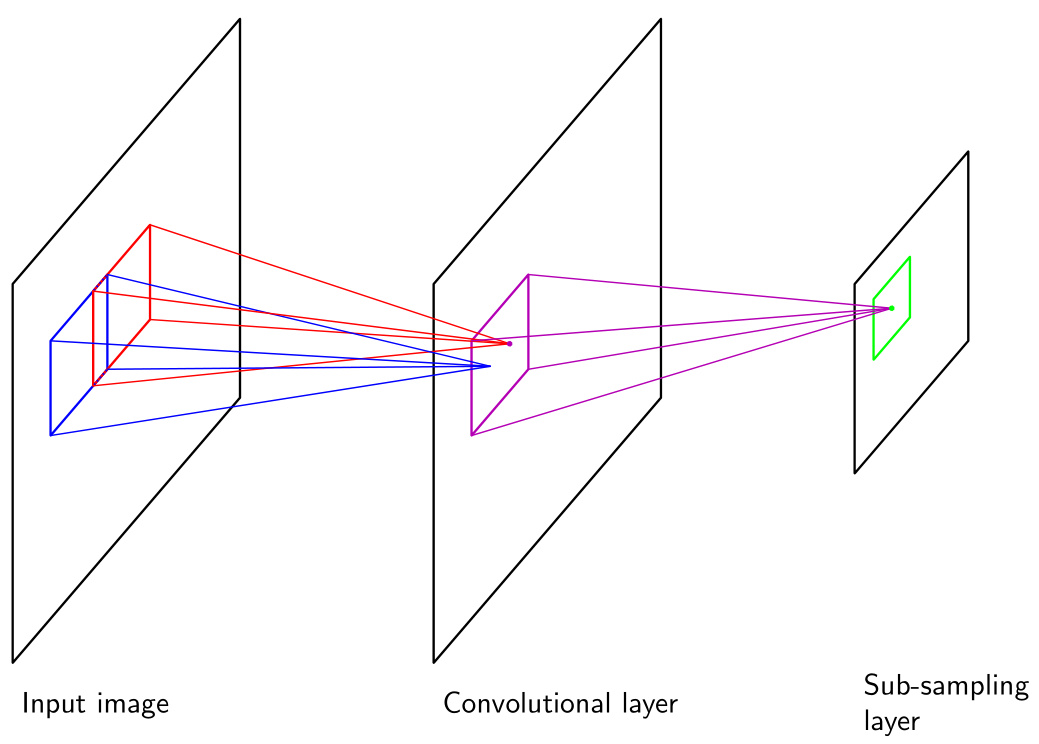
\includegraphics[width = 1.0\textwidth]{./Figures/pattern_recognition_and_machine_learning_CNN.jpg} % SIngle CCN layer
		\rule{35em}{0.5pt}
	\caption[A CNN Layer]{A CNN is made up of many alternating convolution and pooling layers. Each convolutional layer can make use of many kernels. The output feature maps are then subjected to a pooling or sub-sampling layer. A convolution and pooling stack together form one of several successive layers of a CNN.}
	\label{fig:CNN_2}
\end{figure}
\begin{figure}[htbp]
	\centering
		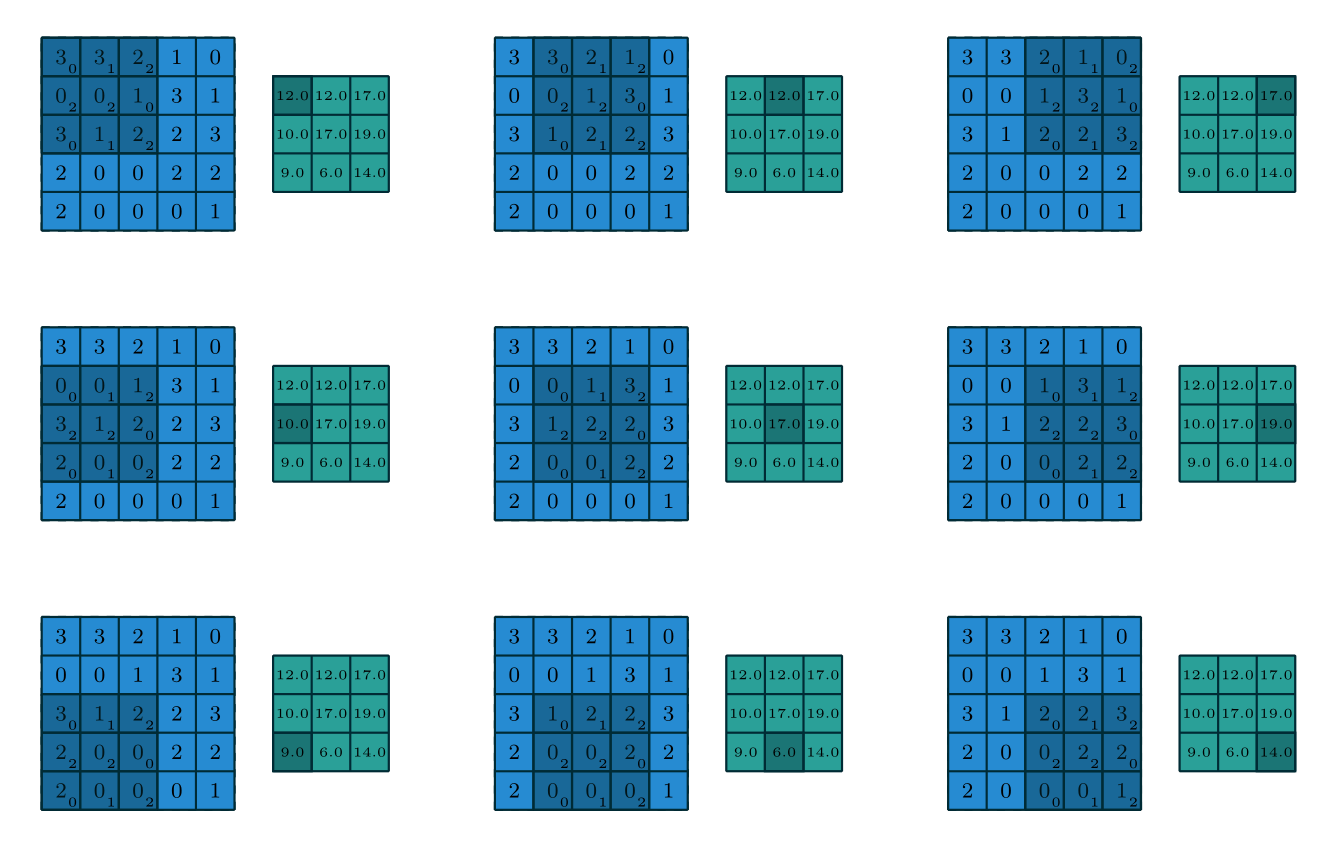
\includegraphics[width = 1.0\textwidth]{./Figures/1603_07285v1_convolving.PNG} %convolving
		\rule{35em}{0.5pt}
	\caption[Convolution]{Activations from layer 1 (shown as the blue grid) are convolved with the kernel (shown by subscript values in the convolution window) to produce a weighted sum for every neuron in the layer above (shown by the green grid). As the kernel size is $3\times 3$, a convolution with a single block stride to all sides will produce a $3\times 3$ grid. This can be altered by padding grid with zeros.}
	\label{fig:Convolution}
\end{figure}

\subsubsection{Pooling}
Following convolution \textit{pooling} is applied.
The role of pooling is to merge semantically similar features into one.
For example, the relative positions of the features forming a alphabetic letter can vary.
A way to reliably detect the feature can be done by coarse-graining (reducing the spacial resolution of) the position of each feature in a manner that preserves relevant information whilst removing sensitivity to noise, translations and distortions\citep{dengthree}\citep{lecun1995convolutional}\citep{bengio2009advances}.

The pooling layer subdivides the convolution layer output into regions of size $z \times z$ known as \textit{pooling windows}\citep{chen2014big}. 
Each window is reduced to a single value with the \textit{pooling function}, see Figure ~\ref{fig:Pooling}.
Pooling windows may be over-lapping but this has empirically been shown increase over-fitting\citep{bengio2009advances}\citep{krizhevsky2012imagenet}.

\begin{figure}[htbp]
	\centering
		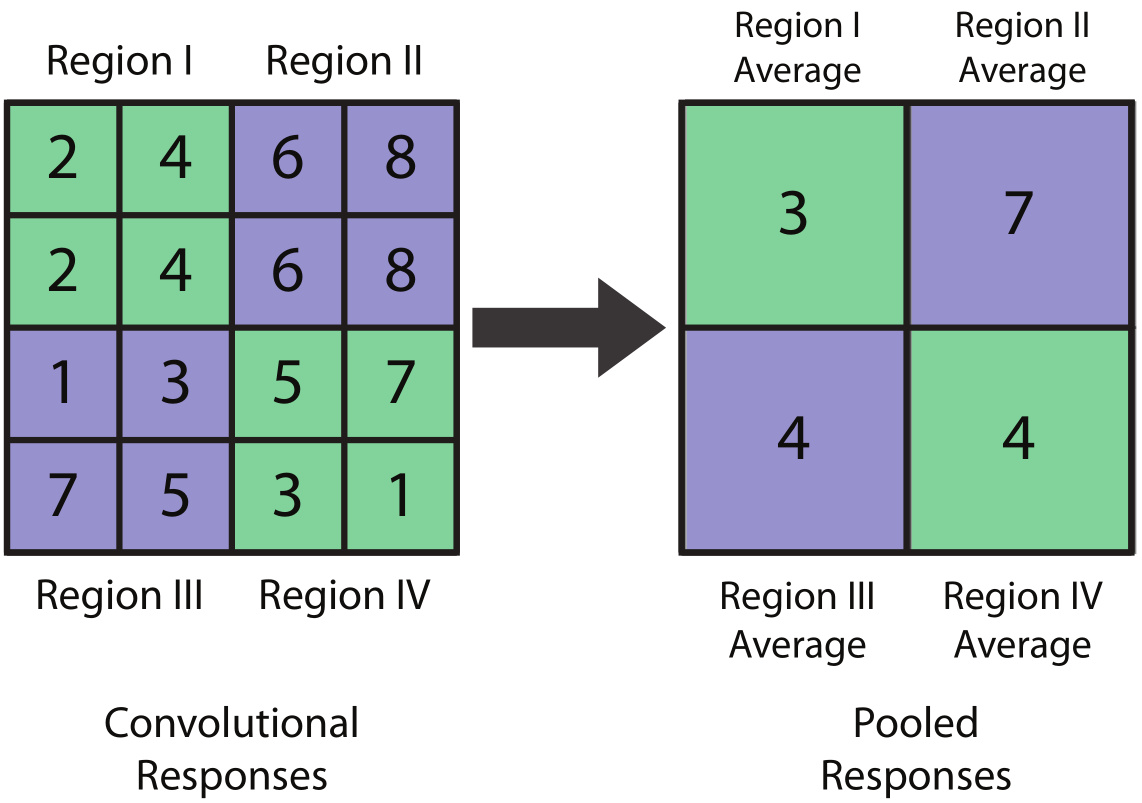
\includegraphics[width = 0.6\textwidth]{./Figures/convolution_end_to_end_recognition_with_cnns.jpg} %Pooling
		\rule{35em}{0.5pt}
	\caption[Pooling]{Convolution responses are pooled with an averaging function using non-overlapping windows.}
	\label{fig:Pooling}
\end{figure}

The net effect of weight sharing in the convolutional layer followed by a pooling scheme provides the CNN with natural translation in-variance properties\citep{dengthree}, see Figure ~\ref{fig:CNN}.
The pooling function is usually \textit{xax-out}.
This is the maximum, $max(f_i)$, where $f_i$ refers to all elements in the pooling window\citep{bengio2009advances}\citep{lecun2010convolutional}.

Maxout serves two purposes:
\begin{enumerate}
\item It picks out the highest activation in a local region, thereby providing a small degree of spatial invariance.
\item It reduces the number of activations for the next layer by a factor of $z^2$.
With a smaller feature-map less parameters to be learnt in the later layers.
\end{enumerate}

Alternatively, the pooling function may be the average, $\sum_i(f_i)/z^2$, as in Figure ~\ref{fig:Pooling}.
Typically pooling window size and stride are hand-designed, however algorithms exist which generate learn-able pooling regions\citep{bengio2009advances}\citep{lecun2015deep}.
\begin{figure}[htbp]
	\centering
		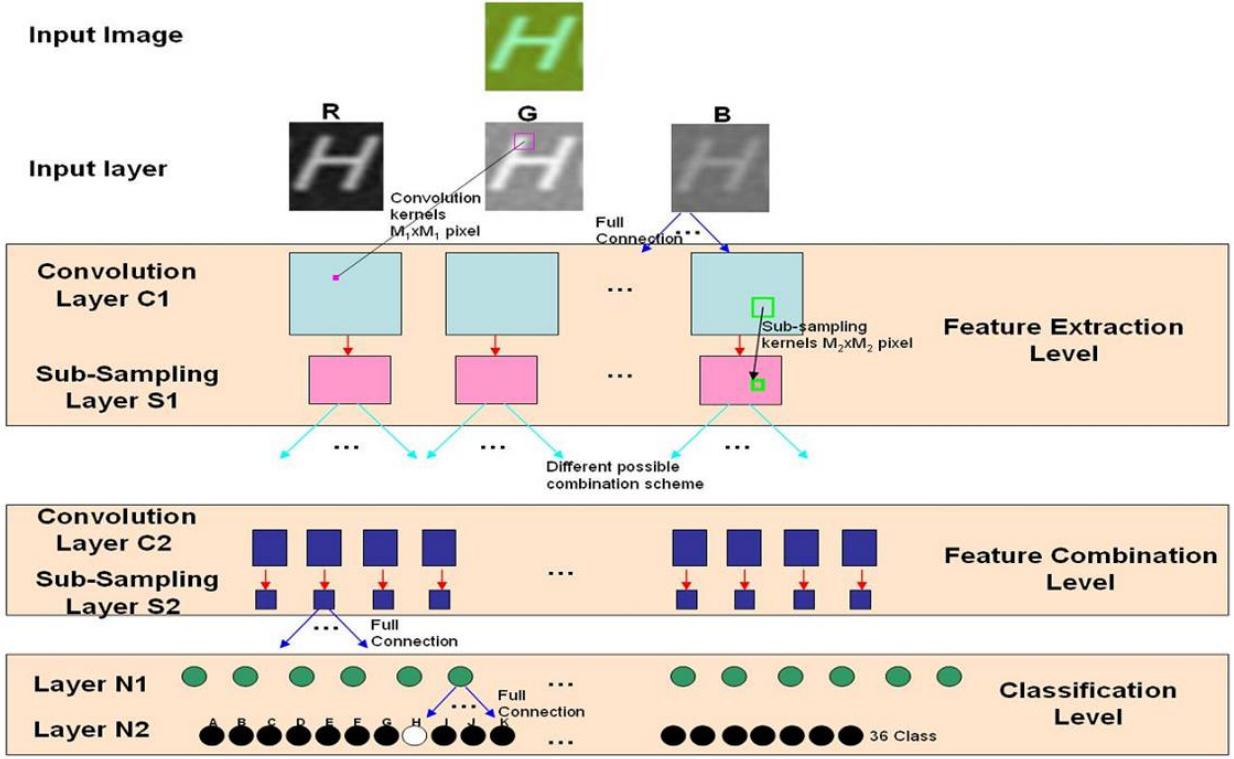
\includegraphics[width = 1.0\textwidth]{./Figures/CNN_network_sparse_coral_classification_3.jpg} %CNN Structure
		\rule{35em}{0.5pt}
	\caption[CNN Architecture]{A standard image will have three layers of intensity values for the red, green and blue pixels respectively. A stacked tensor of RGB values can be convolved with a 3D kernel or, as in the case above, each layer is convolved with a 2D kernel separately. All produced feature-maps are subsequently sub-sampled with pooling. CNN architectures may vary in may ways such as kernel shape, pooling window size, pooling functions and number of layers. After several stages there are many small feature maps. Commonly they are connected to an MLP used for classification or regression tasks.}
	\label{fig:CNN}
\end{figure}

As all kernel weights are learned via back-propagation CNNs can be understood to be synthesizing their own feature generators\citep{lecun1995convolutional}.

\begin{figure}[htbp]
	\centering
		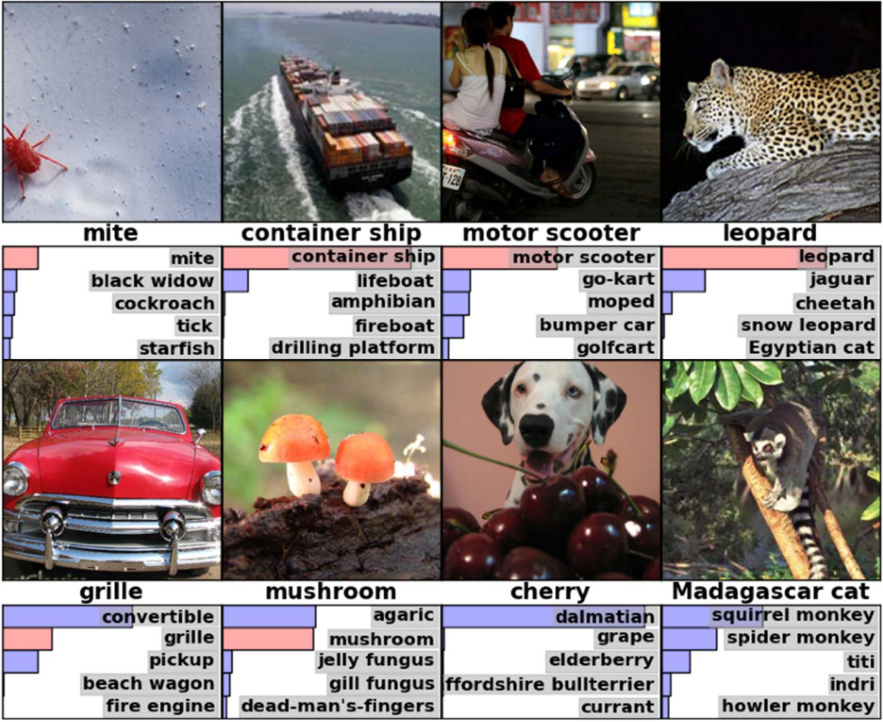
\includegraphics[width = 0.8\textwidth]{./Figures/CNN_image_prediction_krizehevvsky_nips_2012.jpg} %IMAGENET example
		\rule{35em}{0.5pt}
	\caption[Image Recognition]{A CNN was trained as part of the Imagenet Recognition Challenge\citep{deng2012imagenet}. The dataset was composed of approximately 1000 images for each of 1000 categories. Shown above are the top 5 predictions for each of the test images. The model achieves a top-1 and top-5 error rate of $37.5\%$ and $17.0\%$ respectively. A top-5 error rate is the fraction of test-objects not seen in the top five model predictions. Even where the top-1 is wrong the top-5 predictions seem reasonable. In fact, on the bottom row the model appears to be more accurate than the provided labels.}
	\label{fig:Image_predication}
\end{figure}

\section{Measuring Performance}
Two primary sources of data exist when producing a model, a training and test set.
The training data is used to tune the model parameters; the model learns from training data.
However, in order to produce an independent measure of the model's performance a test set must be used.
It may be quite intuitive to think a model's success can be completely measured by the accuracy of predictions on the test set, however this does not tell the whole story.
%Accuracy
%Motivation for Precision Recall F-measure 
%Confusion Matrix
%AUC.
%Critical Evaluation

\subsection{Test Performance Error}
If we measure a model to have an accuracy of $85\%$ this does not tell us how much the true value may differ with different degrees of confidence.
We would be more confident of the accuracy being near the $85\%$ if we got that result from a test set of 10,000 instances than of 100.
We consider the test to be like a Bernoulli process in order to give some measure of confidence.
In statistics, a Bernoulli process is one in which a succession of independent events can have one of two results, like pass or fail, correct or not.

This has a simple method for providing confidence intervals\citep{witten2005data}.
\be
p \pm z \sqrt{\frac{1}{n} p(1 - p)}
\ee
where $p$ is the accuracy estimated from the test set, $z$ is the $1 - \frac{1}{2}\alpha$ quantile often given in the back of many statistical textbooks, and $n$ is the number of samples within the test set.

\subsection{Confusion Matrix} 
If $80\%$ of the test set are dogs, and $20\%$ are not, then a model can get an accuracy of $80\%$ just by guessing `dog' every time; clearly not a very useful model.
This motivates the use of a \textit{Confusion Matrix}.
A confusion matrix is a table counting the occurrences of all the possible model prediction outcomes.
For every classification there are four possible outcomes.
If the model correctly predicts `dog', it is called a true positive (TP); if incorrectly classed as `not a dog' then it is a false negative (FN).
On the other hand, if the model correctly predicts the object to \textit{not} be a dog it is a true negative (TN); but if classified as dog when it is not, then it is a false positive (FP).

We can construct a confusion matrix, also called a \textit{contingency table}, counting all the outcome types from the test set.
Each row in the table refers to the true classes and each column classifier predictions\citep{flach2012machine}, see Figure ~\ref{fig:Confusion_matrix_2}.
\begin{figure}[htbp]
	\centering
		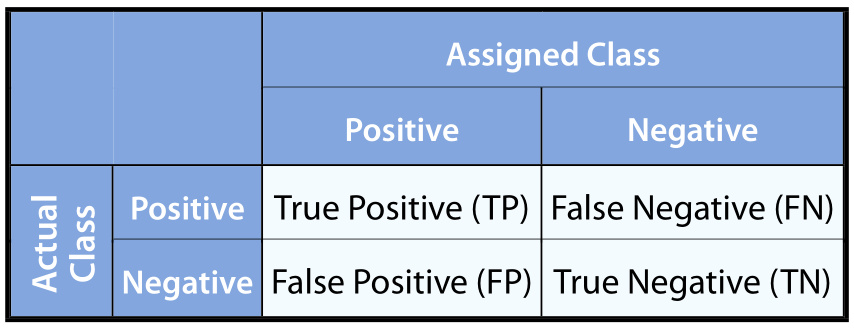
\includegraphics[width = 0.8\textwidth]{./Figures/encyplopedia_of_machine_learning_confusion_matrix.jpg}
		\rule{35em}{0.5pt}
	\caption[Confusion Matrix]{A confusion matrix encapsulates the success of a binary classification model. Ideally all true positive classes will be labelled as positive, \textit{True Positives}; and all negative classes as labelled as negative, \textit{True Negatives}. These will only fill in the tables backward diagonal. The forward diagonal shows cases in which the prediction was incorrect. If predicted positive where truly negative a \textit{False Positive} is committed. Alternatively when predicted negative but truly positive, a \textit{False Negative} has been committed.}
	\label{fig:Confusion_matrix_2}
\end{figure}

From the confusion matrix we can calculate a range of performance metrics.
Accuracy is the simplest
\be
Accuracy = \frac{TP + TN}{TP + TN + FP + FN}
\ee
that is the sum of the correct predictions over the total.

\subsection{Precision and Recall}

Two other useful measures of performance are \textit{precision} and \textit{recall}\citep{flach2012machine}\citep{ball2010data}.
Recall - also known as \textit{Completeness}, \textit{Sensitivity} or \textit{True Positive Rate} (TPR) - is the fraction of objects truly belonging to a category that are correctly classified as such,
\be
Recall = Completeness = Sensitivity = TPR = \frac{TP}{TP + FN} 
\ee

The False Positive Rate(FPR), or `Type 1 error', is the fraction of positive classifications which are incorrect given by
\be
FPR = \frac{FP}{FP + TN}
\ee
which relates to the \textit{Specificity}, or fraction of the negative class correctly classified,
\be
Specificity = \frac{TN}{FP + TN} = 1 - FPR
\ee
\textit{Precision} (also known as \textit{Efficiency}) is the fraction of objects classified as a class that truly belong to that class:
\be
Efficiency = Precision = \frac{TP}{TP + FP} 
\ee

The ideal would be to have both precision and recall to be close to one, however there is often a trade-off between the two.
The preferred balance between precision and recall will be problem-dependent and may hinge on not having too much contamination of the positive class, or the economic costs of incorrect classifications.

In practice Precision and Recall are particularly important measures in the case of \textit{skewed classes}.
Skewed Classes is the scenario in which one class significantly outnumbers the other class or classes in a data set.
For example when detecting fraudulent behaviour in on-line banking, the majority of activity will be normal.
Should a classifier predict the activity is normal all the time (clearly a bad classifier) it will still be right most of the time and score a high accuracy.

\subsection{F-measure}
A measure that combines precision and recall to give an indication of the algorithm's success is the $F_\beta$ measure (for real non-negative values of $\beta$)\citep{sokolova2006beyond}\citep{davis2006relationship}:
\be
F_\beta = \left(1 + \beta^2\right)\frac{precision.recall}{\beta^2.precision + recall}
\ee
The F-score favours Precision when $\beta > 1$, is evenly balanced when $\beta = 1$ and favours Recall where $\beta < 1$.
When balanced we have the \textit{F-measure} or\textit{ balanced F-score},
\be
F_1 = 2\frac{precision.recall}{precision + recall}
\ee
which ranges from zero to one.

\subsection{ROC Curve and AUC Score}
The Receiver Operating Characteristic (ROC) curve is an encompassing visualization of a binary classifier's performance\citep{sokolova2006beyond}\citep{davis2006relationship}\citep{fawcett2006introduction}.
They have long been used in signal detection theory as a way of visualizing and evaluating the trade off between false alarms and correct hits and are commonly used in the design of medical diagnostic tests which are not $100\%$ accurate.
ROC curves are useful because they allow for better analysis of the trade-off between the false positive rate and the true positive rate.

Consider a case of two classes.
Formally each example $E$ is mapped to one of the set $\{p, n\}$ which are positive and negative labels respectively.
The classier or model is a mapping from each example to one of the classes.
Some models will do this by producing continuous output, often a number between $0$ and $1$, to which thresholding is applied.
If the output surpasses the threshold it is classified as $1$, for positive, otherwise $0$ for negative.

The ROC curve is a plot of TPR on the Y-axis vs FPR on the X-axis.
For a model that produces continuous output, by changing the threshold you can obtain many pairs of $(TPR, FPR)$ values which on a scatter-plot produce an \textit{ROC curve}, see Figure ~\ref{fig:ROC_curve_2}.
For a model that has discrete output, even before any threshold, this will only be a single point on the graph corresponding to the only $(TPR, FPR)$ pair.
Such discrete scoring classifiers can often have their internal state converted into a score rather than a discrete outcome which will provide a full ROC curve.
An example of this is in the decision tree algorithm that produces its discrete output based on the proportion of one instance over another at the final node.
By just using the ratio, and not choosing the most common label you have a continuous score.
\begin{figure}[htbp]
	\centering
		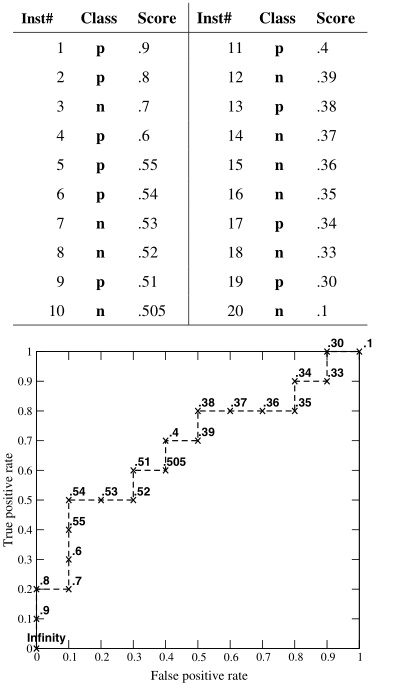
\includegraphics[width = 0.7\textwidth]{./Figures/ROC_curve.jpg}
		\rule{35em}{0.5pt}
	\caption[The ROC Curve]{A classification model that produces continuous output can vary in performance based on the threshold chosen. To provide an unambiguous measure a Receiver Operating Characteristic (ROC) Curve is used. In the example above continuous scores have been assigned to each of the 20 instances where their true class is known. The curve is made by plotting the True Positive Rate (TPR) vs the False Positive Rate (FPR) for all possible threshold values (shown above the crosses). The final threshold selected is problem-dependent. In general terms a model with ROC curve that hugs the $(0,1)$ point is preferred.}
	\label{fig:ROC_curve_2}
\end{figure}

The ideal model should go through the point $(0, 1)$, that is where there are no false positives and a $100\%$ true positive rate.
Classifiers that appear toward the left hand side of the plot can be thought of as conservative, in that they require strong evidence to make a positive classification.
However, their stringent criteria will make few examples classified as positive.
Classifiers appearing toward the upper right are quick to label an example as positive, so they are likely not to miss positive classifications.
Their lax criteria will likely contaminate the pool of positives with many incorrectly labelled negatives.
As there are generally more negative cases than positive, more non-cats then cats, behaviour of the ROC curve toward the upper left tends to be the most informative.

If a models ROC curve lies along the 45 degree $y = x$ line it means the classifier is either randomly guessing, or it has not learned a useful data representation.
For example ,if it guesses positive half of the time it will have a TPR equal to $0.5$, however as now half of the negatives will be incorrectly classified the FPR will equal $0.5$ as well.
This $TPR = FPR$ trend will be true for any percentage of a random example being positive, yielding a line along $y = x$.
In fact, if the proportion of positive to negative classes changes an ROC curve will not be affected at all.
This insensitivity to skew classes is what makes ROC curves so useful.
Classes that outnumber their opposite class are very common in real world problems making a performance measure invariant to skewness even more valuable.
In some cases the skewness of classes may alter with time, such as the number of infected people over time, but that should not change the fundamental characteristics of what identifies someone as infected by a disease.
Should a model appear below the $y = x$ line this means it performs even worse than random guessing.
This is not necessarily a bad thing as the model has captured a useful data representation but is making incorrect conclusions.
Should label predictions be swapped around, positive to negative and vice versa, the model performance is improved.

It will often be the case that the most natural threshold of $0.5$, for a model output between $0$ and $1$, is not the best.
Depending on the model and the problem it may be that selecting the threshold to be $0.6$ has a better TPR without increasing the FPR.

A common way of comparing models to each other in a single measure is to use the \textit{Area Under an ROC Curve} (AUC), see Figure ~\ref{fig:AUC_score}.
A perfect classifier would reach a TPR of 1 and FPR of 0, so the curve would be a straight line along $TPR = 1$ with an area underneath of 1.
A classifier that performs no better than random, a line of $y = x$, would score half of the total area, $0.5$.
It is still possible for a model with a lower AUC score to perform better than a model of higher AUC score in a particular domain.
Therefore, one should not necessarily select the model with the highest AUC score as it depends on the costs of true positives and a false negatives.
For example, if astronomers make a classifier of abnormal galaxies in order to follow them up with further study, it is more important to have a high TPR, even at the risk of weeding out some abnormal galaxies, than it is to have a low TPR but high FPR.
If there are a large number of false positives the data set is essentially contaminated with a large pool of galaxies the astronomers cannot afford telescope time to waste on.
Here fewer positives of high quality is better than many positives of low quality.
So if a model happens to perform best in the ROC region of interest even though it has lower AUC score it would be the `economical' choice.
\begin{figure}[htbp]
	\centering
		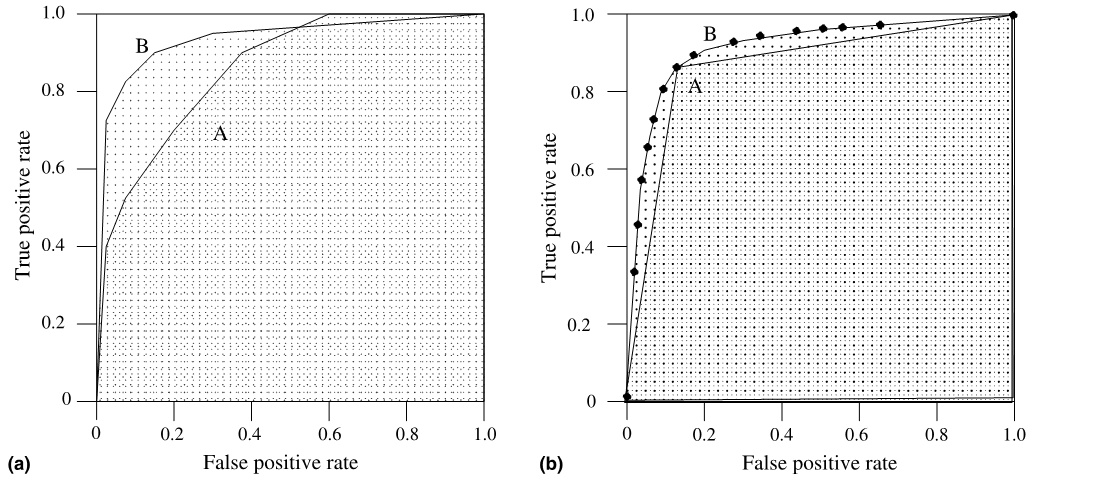
\includegraphics[width = 1.0\textwidth]{./Figures/AUC_measure_introduction_to_roc_analysis_2.jpg}
		\rule{35em}{0.5pt}
	\caption[The AUC Score]{The Area Under Curve (AUC) score is the area under the ROC curve. A perfect model will have an area of 1 $unit^2$. This measure is better for evaluating the general performance of one model vs another when the model with higher TPR may vary depending on the FPR domain.}
	\label{fig:AUC_score}
\end{figure}

Selecting the model with the highest AUC score suffers from the same problem as picking a model of higher accuracy.
Without a measure of the variance this score can only be trusted so much.
This can be done by testing on multiple test sets generated via cross-validation and then averaging.

\section{SDSS Survey}
This section supplies the necessary knowledge of supernovae for this thesis.
Following this machine learning as a tool for handling astronomy data is discussed.
Thereafter, we discuss the Sloan Digital Sky Survey (SDSS), the objectives, data and current methodology for data handling.
As a potential solution to data handling problems of modern astronomy this thesis proposes the use of deep learning techniques as superior to the more classical machine learning methods.
In this light we discuss results for prior work on the application of machine learning to supernovae detection.
%Supernovae
%Transient Types

%The LDSS Survey
%Data origin

%Difference Imaging
%State of other research
%Critical Evaluation

%Data Specs
%Fakes
%Specto Confirmed
%Data Splitting
\subsection{Supernovae}
A supernova (SN), illustrated in Figure ~\ref{fig:supernovae}, is a powerful explosive event at the end of a stars lifetime\citep{du2014machine}.
In fact so much energy is released that the star briefly outshines the host galaxy\citep{baade1938photographic}.
Different supernovae (SNe) types may be classified by their spectral features.
Type I SNe have no hydrogen lines, unlike Type II SNe which do.
Type 1 may be broken up into a three subtypes: Type Ia have strong signatures of higher-mass elements such as silicon, sulphur, iron and calcium but little of hydrogen and helium; Type Ib have prominent helium lines and Type Ic have neither hydrogen nor helium.
The features arise from differences in the explosion source.
Type Ia are the result of the thermonuclear explosion of a white dwarf, which is the last stage of many stars' lifetimes where the envelope of gases has been expelled to reveal a degenerate core - extremely dense matter that is supported from collapsing in on itself by the Pauli exclusion principle.
%Add reference
The other types, Ib, Ic and II, are the result of a star's core collapsing in on itself.
\begin{figure}[htbp]
	\centering
		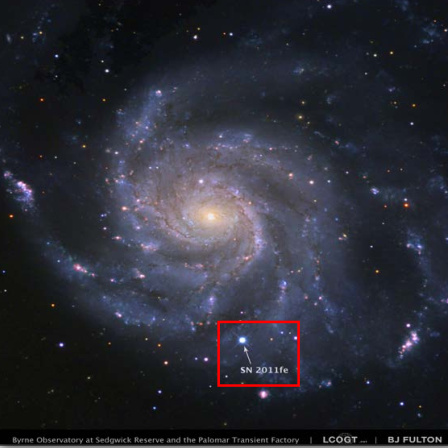
\includegraphics[width = 0.8\textwidth]{./Figures/encyplopedia_of_machine_learning_SN.jpg}
		\rule{35em}{0.5pt}
	\caption[Supernovae]{An image captured by the Palomar Transient Factory of the Pinwheel Galaxy (M101) shows a single exploding star (framed in red), a \textit{supernova}, which can outshine an entire galaxy.}
	\label{fig:supernovae}
\end{figure}
\begin{figure}[htbp]
	\centering
		\includegraphics[width = 0.8\textwidth]{./Figures/lise_thesis_SDSS.jpg}
		\rule{35em}{0.5pt}
	\caption[Supernovae Types]{There are several classes of SNe. Type Ia originate from the nuclear explosion of a low mass star and has consistent light curves. Their spectra have no hydrogen but contain silicon. Type Ib has helium unlike Ic, but both lack hydrogen and silicon. Type II is the only type with hydrogen. Type Ib, Ic and II all originate from core collapse of a massive star and vary greatly in light curve features.}
	\label{fig:supernovae_types}
\end{figure}

A Type Ia occurs in binary systems where two stars, a white dwarf and a larger companion star, orbit one another.
If the companion star enters its red giant phase 1 it starts to inflate to a point where some matter can no longer be bound.
The free matter leaking off the red giant is then slowly accreted by the white dwarf.
The white dwarf's mass will increase, but it cannot do so indefinitely as the nuclear forces preventing collapse can only handle so much.
Once the Chandrasekhar limit ($1.4M_{\odot}$, where $M_{\odot}$ denotes solar mass) is reached the core collapses resulting in a thermonuclear explosion which destroys the star within seconds leaving an expanding gaseous remnant rich in metals.
The remaining supernovae types occur when a massive star ($M > 9M_{\odot}$) can no longer withstand its own gravitational pressure and collapses.
The imploded core can remain either as a neutron star (usually in the form of a pulsar) or collapse further into a black hole, or it can be entirely destroyed.
Supernovae differ not only in spectra but light curves too.
A light curve is a plot of a supernova's intensity over time.
The light curves of types Ib, Ic and II SNe can vary substantially depending on the progenitor's metallicity and mass, as shown in Figure ~\ref{fig:supernovae_curve_types}.
As a Type 1a occurs when a white dwarf accretes exactly the right mass their light curves are typically brighter and have very similar light curves.
\begin{figure}[htbp]
	\centering
		\includegraphics[width = 0.9\textwidth]{./Figures/lise_thesis_light_curves_of_SN.PNG}
		\rule{35em}{0.5pt}
	\caption[Supernovae Light Curves]{Star mass, metallicity and other factors cause SNe to have different light curves. Even within different SNe types there is variation with the exception of Type Ia. }
	\label{fig:supernovae_curve_types}
\end{figure}
It is for this reason that Type Ia SNe are particularly useful for cosmologists to measure distance.
The further away the SN the dimmer it will appear.
In addition, the obtained spectra will be appropriately red-shifted in accordance with their recession from us due to the expansion of the universe.
If one knows how bight a candle burns and how dim it appears one can tell how far away the candle is.
Type Ia light curves and spectra allow for exactly this on a cosmological scale, making them `standard candles', see Figure ~\ref{fig:light_curves}.
In this manner the accelerating expansion of the universe was discovered\citep{riess1998observational}\citep{perlmutter1999measurements} which has since motivated even larger supernovae surveys.
\begin{figure}[htbp]
	\centering
		\includegraphics[width = 1.0\textwidth]{./Figures/lise_paper_light_curves.jpg}
		\rule{35em}{0.5pt}
	\caption[SNe Ia Light Curves]{A Supernova event can be seen for weeks. A time-series of the light intensity is known as a \textit{light curve}. For Type Ia, the trigger conditions are so similar as to produce nearly the same light curves viewed at the same distance. As they are equivalently as bright as one another the change in flux, and Doppler shifted light-curves can be used to infer their distance; making them very useful \textit{standard candles}\citep{branch1992type} in cosmology. }
	\label{fig:light_curves}
\end{figure}

\subsection{The SDSS Survey}
%What is the SDSS
The Sloan Digital Sky Survey (SDSS-II) is a multi-spectrum spectroscopic red-shift survey run during three-month campaigns in the Fall of 2005, 2006, and 2007 as part of the extension of SDSS-I.
The SDSS-II SNe Survey was commissioned to address the following goals\citep{abazajian2009seventh}:
\begin{enumerate}
\item Refine the SNe Type Ia Hubble diagram.
At the time the Hubble diagram  was constructed from low - $(z \approx 0.1)$ and high-red-shift $(z \approx 0.3)$ Type Ia samples from multiple telescopes of differing passbands and selection criteria, introducing systematic errors.
The SDSS-II SNe Survey would gather distance estimates for Type Ia SNe in the sparsely populated red-shift range $0.05 < z < 0.35$ to better constrain the Hubble parameter.
\item Minimise SNe systematics.
At the time most SNe surveys had systematic errors comparable to their statistical errors.
Systematic errors in the SDSS-II SNe Survey would be significantly reduced.
Photometric calibration errors of $1\%$ in Stripe 82 were achieved from the many years on the large-scale calibration of the data during SDSS-I.
In addition, the spectroscopic filters had well measured transmission curves and were all situated on the same stable camera.
\item Fix rest-frame ultraviolet light curves.
SNe at red-shift $z > 1$ have their light curves matched to templates of the rest-frame light curve to reduce systematic errors.
For example the 3600 \AA (the u-band) in the SN rest-frame corresponds to $ \approx 8000$ \AA at a red-shift of $1.2$.
At very far red-shift, $z = 0.3$, the SDSS would be capable of observing this region at $4700$ \AA, the g-band.
The measurements can then be used to improve template data in the rest-frame ultraviolet region.
\item Explore photometric methods to measure SNe characteristics.
Spectra measurements of candidates are a luxury available only when other telescopes have free time and favourable conditions.
The SDSS large depository of photometric data would allow a search for a more practical photometric method of SNe classification and red-shift determination.
\item Study SNe types, rates and host galaxies.
SNe rates of occurrence per galaxy could be estimated for the different SNe types.
In addition, the SNe host galaxies identified could be studied for information about progenitor properties.
\item Finally, SDSS-II would serve as a probe for rare and interesting objects as yet unknown to astronomy.
\end{enumerate}

%Operation
The SDSS 2.5 m telescope and imaging camera are located at the Apache Point Observatory in New Mexico which produces photometric measurements in each of the $u$, $g$, $r$, $i$ and $z$ spectrum filters spanning wavelengths 350 to 1000 nm.
SNe are difficult to detect in the $u$ and $z$ filters except at low red-shifts ($z \approx 0.1$ for Type Ia) due to the relatively poor filter throughput.
Beyond a red-shift of 0.4, Type Ia can still be detected, but after $z \approx 0.2$ the ability to obtain high-photometry quality deteriorates quickly.
During the survey the camera is operated under a ``rolling search''.
This is where a portion of the sky is repeatedly scanned to discover new SNe and measure their respective light curves in the intermediate red-shift range of $0.05 < z < 0.35$.

%Camera 
The SDSS telescope camera, illustrated in Figure ~\ref{fig:sdss_camera}, is comprised of six sensor columns each of which contains five CCD chips corresponding to the $r$, $i$, $u$, $z$ and $g$ filters, see Figure ~\ref{fig:band_efficiencies} for corresponding frequency sensitivities.
The telescope is oriented such that a patch of sky drifts through the cameras field of view; known as \textit{drift-scanning}.
The focused image will drift across the columns providing 55 seconds worth of exposure to each CCD.
Sensor readings for a single point in the sky cannot be taken simultaneously as not all CCD’s are exposed to that point.
Instead CCD’s are read out in sync with the drifting i.e. 55 seconds apart.
Such drift scanning allows the telescope to image long continuous strips of the sky.
\begin{figure}[htbp]
	\centering
		\includegraphics[width = 0.8\textwidth]{./Figures/lise_paper_sdss_camera.jpg}
		\rule{35em}{0.5pt}
	\caption[SDSS Camera]{The SDSS photometric camera has five CCD chips for each of the $riugz$ bands in each of six sensor columns. The camera is oriented such that by the natural rotation of the sky the point of exposure drifts down over the column, taking 55s to cross over each of the rows. }
	\label{fig:sdss_camera}
\end{figure}
\begin{figure}[htbp]
	\centering
		\includegraphics[width = 0.8\textwidth]{./Figures/SDSS_EDR_band_effieciency.jpg}
		\rule{35em}{0.5pt}
	\caption[Response Curve]{The upper curves are the quantum efficiencies for light absorption for each of the $ugriz$ filters ignoring atmospheric effects. The lower curve includes the atmospheric effects assuming an air mass - the optical path length through Earth's atmosphere - of 1.3. Further scattering within the chips affects only the $r$ and $i$ bands with the corresponding response curve given by the dashed lines.}
	\label{fig:band_efficiencies}
\end{figure}

%Location
Exposure time per unit area limits the survey from operating over the whole sky.
Instead only Stripe 82, shown in Figure ~\ref{fig:sky_coverage}, was observed.
This is a 300 $deg^2$ area along the celestial equator, 2.5 deg wide in Declination and between Right Ascension of 20 h and 04 h.
It takes about two nights to cover all of Stripe 82 in this way.
However, the average \textit{cadence}(frequency of observation) was approximately four nights as a result of bad weather conditions and interference from moonlight.
Stripe 82 was used to take advantage of the already extensive object databases, reference images and photometric calibration created by SDSS-I.
As both surveys used the same telescope for photometrics this minimised systematic errors that may occur from differing photometric standards on different telescopes.
\begin{figure}[htbp]
	\centering
		\includegraphics[width = 0.7\textwidth]{./Figures/SDSS_EDR_sky_coverage.jpg}
		\rule{35em}{0.5pt}
	\caption[SDSS Coverage]{The SDSS survey is limited in the area of the sky that it can scan by both being ground-based and requiring long exposure times. Shown above is Stripe 82 which was scanned roughly every four nights.}
	\label{fig:sky_coverage}
\end{figure}

%Difference Imaging
SDSS imaging software\citep{stoughton2002sloan} was used to process the raw images and SNe were identified via a frame subtraction technique\citep{alard1998method}).
Each picture of the sky, the \textit{Search Image}, would be subtracted from the most recent previous image of the sky, the \textit{reference image} in the same position, see Figure ~\ref{fig:transient_detection}, resulting in a \textit{Difference Image}.
This was only done in real-time using the $g$, $r$ and $i$ bands, as they are most useful for SNe detection.
Using just 3 bands allows for more easily interpretable false-colour RGB image to be made.
Unless a transient occurred, this will leave a pure noise image.
The SNe candidates would then be filtered by an automated object detection algorithm requiring that difference images have a noticeable difference detected in two or more filters, not coincide with existing catalogued stars or variable objects, and were not seen to be moving during the $r$ and $g$ band exposures.
In 2006 and 2007, further software cuts were made to lessen the number of images for hand scanning.
The change significantly reduced the number of moving objects, diffraction spikes, and long-term variable objects by cross-matching with a veto catalogue.
Now, single-epoch detections would be sent on-wards to manual scanners if they were not moving, bright enough ($M_r < 21$ or $M_g < 21$) and detected in at least two epochs.
\begin{figure}[htbp]
	\centering
		\includegraphics[width = 1.0\textwidth]{./Figures/Transient_detection_The_difference_imaging_pipeline_for_the_transient_search.jpg}
		\rule{35em}{0.5pt}
	\caption[Transient Classification]{A difference images is produced by subtracting a new image from a reference image. Should a peak with large signal to noise ratio be detected it is a transient. Shown above is the difference image for the $i$-band in deep field C3 on 13 October 2013. Noted transients are outlined (in red) below. Outlined in dashed red-boxes are objects that failed initial detection cuts. Objects in solid red boxes passed the cuts but were then ruled out by an \textit{autoScan} algorithm. The objects outlined in yellow circles path both tests and are potential SNe candidates.}
	\label{fig:transient_detection}
\end{figure}

%Detection
In the past, removal of false detections was done manually by astronomers, see Figure ~\ref{fig:hand_scanning} for the decision-tree.
During hand scanning, obvious artefacts such as in Figure ~\ref{fig:transient_examples} were removed.
Artefacts can be produced via diffraction spikes, CCD saturation, bleeding and registration errors among others.
However, this hand-scanning process was imperfect and led to a large number of artefacts that constituted $70\%$ or more of the candidates.
A team of roughly twenty hand scanners used the $g$, $r$ and $i$-band search and difference images (each having a size of $51 \times 51$ pixels) and object history to classify each of the candidate objects into one of ten possible classes: dipoles, artefacts, saturated stars, transients, variables, moving objects, SN Gold, SN Silver, SN Bronze and SN Other\citep{frieman2007sloan}.
For SDSS-II supernova survey, this meant hundreds or thousands of images being manually scanned each night.
Unfortunately it has been found that classification is done inconsistently between people or even the same person over time depending on mood and exhaustion.
\begin{figure}[htbp]
	\centering
		\includegraphics[width = 0.9\textwidth]{./Figures/lise_paper_hand_scanning.jpg}
		\rule{35em}{0.5pt}
	\caption[Hand-scanning]{Hand-scanners labelled the transients in the dataset according to the decision tree above.}
	\label{fig:hand_scanning}
\end{figure}

Even if the transient is genuine it may not be a SN but an asteroid, variable star, cosmic ray or artificial satellite, see Figure ~\ref{fig:transient_examples} for some examples.
\begin{figure}[htbp]
	\centering
		\includegraphics[width = 1.0\textwidth]{./Figures/transient_examples_Real-time_detection_of_transients_in.jpg}
		\rule{35em}{0.5pt}
	\caption[Artefacts]{Many apparent transients are imaging artefacts or are not supernovae. Each of the difference images above show artefacts and their source of occurrence.}
	\label{fig:transient_examples}
\end{figure}

Figure ~\ref{fig:transient_types} shows a summary of the many different genuine transients.
Should other telecopes be available they can be used to validate the remaining SNe candidates\citep{adelman2008sixth}.
\begin{figure}[htbp]
	\centering
		\includegraphics[width = 1.0\textwidth]{./Figures/Transient_types_Thirty_metre_deatiled_science_case.jpg}
		\rule{35em}{0.5pt}
	\caption[Transient Variability]{The variability tree summarizes the potential sources of detected transients.}
	\label{fig:transient_types}
\end{figure}

As hand-scanning accuracy is paramount, fake SNe were injected into the pipeline to provide quality control and calculate the average detection efficiency per human\citep{kessler2015difference}\citep{dilday2008measurement}.

%Research Motivation
Regardless of human accuracy, eye-scanning of future sky surveys such as the Large Synoptic Survey Telescope (LSST) will not be possible due to the millions of detections per night.
The LSST is expected to find 1,000 new supernovae each night for 10 years; at least a million Type Ia SNe over its lifetime, effectively generating one SDSS each night\citep{abell2009lsst}\citep{mickaelian2015astronomical}.
Such Big Data demands new statistical inference and machine learning techniques for processing and analysis.
This concern is what motivates this dissertation on applying Deep Learning techniques to the detection of SNe.

%Data Specs
Throughout the SDSS-II SNe Survey 10,258 new variable objects were discovered and 500 Type Ia were spectroscopically identified including 81 core-collapse SNe.
The final data release was of all transient sources brighter than $\approx 22.5$ mag that had no known variability prior to 2004 and excludes known active galaxies.
The obtained full data-set contains 27,480 objects of which 11,959 are not-real and 15,521 are real.
Data from 2005 were omitted because of the different threshold cuts employed at the time so as not to introduce unnecessary variation into the data-set.
For classification purposes, the original classes were regrouped into three new visual classes, ``artefacts'', ``real objects'' and ``dipoles/saturated''.
Residuals of real objects are point-like (convolved with the telescope and atmosphere’s seeing), artefact residuals resemble diffraction spikes and dipoles/saturated objects are often quite point-like, typically with negative flux in some part of the image stemming from saturated CCD effects or registration errors.

\subsection{Previous Results}
%Prior Research
Prior work on automatic classification has been done as part of the SNe factory where difference image attributes such as position, shape, Full Width Half Maximum (FWHM) and distance to the nearest object in the reference image are used to discriminate between fakes and transients\citep{bailey2007find}\citep{romano2006supernova}.

Recently several `classical' machine learning algorithms to the classification of candidate SNe\citep{du2014machine}.
These include Naive Bayes(NB), Support Vector Machines(SVM), K-Nearest Neighbours(KNN), a three layer MLP(using the python SkyNet package), Minimum-Error Classification(MEC) and Random Forests(RF).
The features used in all these algorithms were derived with several data-reductions methods.
Principal Components Analysis(PCA)\citep{jolliffe2002principal} performs an orthogonal rotation in the complete feature space such that the first axis of the new set of co-ordinates, or the first principle component, is oriented in the direction of greatest variance.
The second PCA component direction will have less variance and so on.
In doing so this also removes any linear correlation between PCA components.
Each sample in the dataset can be entirely described by using the $N$ PCA co-ordinates instead of the original $N$ features.
However, the reducing variance of the PCA components means that earlier PCA components likely carry more information.
If only the first $M$ components are used and the remaining $N - M$ components discarded then the number of features can be severely reduced without losing much information.
Five different feature sets were made with 0, 5, 10, 25, 50, 100 and 200 PCA components respectively.

In addition to PCA, another feature reduction method called Linear Discriminant Analysis(LDA) was used. %reference LDA
LDA projects the data in a direction that maximises the variance between classes and minimises the variance within a class.
LDA can only produce $\leq n_{classes} - 1$ and so can only produce a few components.
As there are only two classes (real and non-real) each object had only one LDA component as a feature.

By creating feature sets with the varied number of PCA components from the original $51\times 51$ image or the central $31\times 31$ image, either including or excluding the LDA component and using either normalized or non-normalized versions a total of 56 data-sets were created.
During training the choice of data-set was treated as a hyper-parameter to be optimized by cross-validation.
Using this exhaustive process to create feature sets the results are shown in Figure ~\ref{fig:classic_result}.

\begin{figure}[htbp]
	\centering
		\includegraphics[width = 0.7\textwidth]{./Figures/classic_ML_result_lise_paper.jpg}
		\rule{35em}{0.5pt}
	\caption[Previous Results]{The ROC Curve and corresponding AUC scores for `classic' machine learning methods on the SDSS dataset\citep{du2014machine}.}
	\label{fig:classic_result}
\end{figure}

The performance results for each of the classifiers on the fake sub-set of SNe is listed in Figure ~\ref{fig:fake_result}.
\begin{figure}[htbp]
	\centering
		\includegraphics[width = 0.45\textwidth]{./Figures/lise_paper_results3_fake.PNG}
		\rule{35em}{0.5pt}
	\caption[Fake SNe QA]{Previous performance results on the fake sub-set of SNe.}
	\label{fig:fake_result}
\end{figure}

Performance on the spectroscopically confirmed SNe sample are shown in Figure ~\ref{fig:spectro_result}.
\begin{figure}[htbp]
	\centering
		\includegraphics[width = 0.5\textwidth]{./Figures/lise_paper_results_spectro.PNG}
		\rule{35em}{0.5pt}
	\caption[SNe confirmed QA]{Previous results by on the spectroscopically confirmed SNe.}
	\label{fig:spectro_result}
\end{figure}

Whilst these results are impressive, deep-learning offers to bypass the laborious creation of feature sets and CNNs have shown impressive results on image recognition tasks.
The rest of this dissertation will focus on the application of CNNs to the data-set in an effort to improve the current state-of-the-art.

To make the clearest comparison between previous results\citep{du2014machine} and this research the exact same data-split was used.
25\% is reserved for the test-set and 75\% of the remaining data is used for training leaving the rest for cross-validation.
% Chapter 1

\chapter{Research Design} % Main chapter title

\label{Chapter2} % For referencing the chapter elsewhere, use \ref{Chapter1} 

\lhead{Chapter 2. \emph{Research Design}} % This is for the header on each page - perhaps a shortened title

%----------------------------------------------------------------------------------------



\begin{comment}
You should begin the Research Methodology chapter by stating, again, the
research objectives of the project. This will enable the reader to make an
assessment as to the validity of your chosen research methodology. 
 
The methodology section should discuss what methods you are going to use in order to
address the research objectives of your dissertation.
Research Design – describes the methods that will be used to collect data or organize
creative products. May include the following depending on the department:
a. Description of the design
leave no question as to the procedures used to complete the study. 
You need to justify why the
chosen methods were selected as the most appropriate for your research, amongst the
many alternative ones, given its specific objectives, and constraints you may face in
terms of access, time and so on. Reference to general advantages and disadvantages of
various methods and techniques without specifying their relevance to your choice
decision is unacceptable. Remember to relate the methods back to the needs of your
research question.

b. Criteria for judging credibility and trustworthiness of results (where relevant)
9. Sampling – describe the aspects of the cases on which data collection and analysis will
focus (where relevant)
a. Indicate how access to the study population will be achieved
10. Variables – describe aspects of the cases on which data collection and analysis will focus
(where relevant)
11. Methods of Data Collection – explain how each variable will be measured (where
relevant)
12. Data Analysis Procedures – describe



The conclusion of this chapter should provide a summary of the main points
that have been covered. The conclusion should also direct the reader as to how
the contents of this chapter link in with the contents of the next chapter, your
findings. This chapter will be usually be between 1,000 and 2,000 words.
\end{comment}





%Data summary 
%Fits Files
%gri bands
%what is measured.



Many things to investigate

Diff/ and Search Images
Data normalization
No. Layers
filters per layer,
filter size
Pooling 
Dropout

Weight initializaton
learning rate
loss fucntion

Batch norm
optimizers
l1 and l2 regularization
patience
no epoch
activations
number of neurons in final layers
Batch size
Data Augmentation:
	


Binary vs Multiple Classifiaction


Computing resources
floating point operations
Theano
Keras
Sklearn
cnmem
fastmath
cudnn
skimage
theano
numpy
pyfits
tsne
buffering on CPU

SKA server (4 Titan X GPUs)



% Chapter 1

\chapter{Results} % Main chapter title

\label{Chapter3} % For referencing the chapter elsewhere, use \ref{Chapter1} 

\lhead{Chapter 3. \emph{Results}} % This is for the header on each page - perhaps a shortened title

%----------------------------------------------------------------------------------------
\begin{comment}
Order of Presentation
Offer your results in an order that is similar to the order you presented your
hypothesis or research questions.

Descriptive Data
Provide all the descriptive data such as demographic results.

Results of Statistical Testing
Give the results of the statistical processes conducted for your study. Provide
only the results and avoid offering conclusions or interpretations of the results.

Interpretations of Statistical Results
Offer a brief summary of the results with foundational interpretations of what the
statistics provide.






This chapter presents the evidence and/or results of primary research which
you have undertaken. 
Depending upon your subject area this can be in the form
of detailed quantitative models, hypothesis testing to some basic analysis using
basic descriptive statistics or qualitative techniques dealing with structured
content analysis, textual analysis, to case study descriptions.
The main part of the chapter is the presentation of the data that you obtained.
Even projects of relatively moderate dimensions will generate a large amount
of data which has to be considered. 
This data must be organised in a logical
and coherently ordered whole so that your thought processes and
interpretation are clear to the reader.
Whatever form of data analysis has been undertaken, it must be accomplished
with care and attention to detail, as should the way in which the results are
presented. 
Nothing is guaranteed to frustrate a reader more than to have to
plough their way through an arid mass of tables, figures and statistics. Better by
far to describe in an accessible manner (which does not mean that you should
talk down to the reader) what the research has uncovered and to include only
the most pertinent figures as evidence of your findings. 
Dissertations which
included detailed modelling or quantitative analysis will clearly need to show
all relevant assumptions, relationships and methods. Your academic supervisor
will be able to advise on the level of detail required in the main body as
opposed to that included in the Appendix.
Graphs, diagrams, pie-charts etc. are all useful ways of presenting research
results; they are an imaginative way of ‘breaking up’ solid blocks of text – they
let a little ‘light’ into the body of the text as long as they are relevant and
illustrate your points. 
Keep your review to those items which are relevant to
your research question and not just everything I found out.
There will be problems in the execution of any research project and their
occurrence should be brought to the attention of the reader. 
Without stating
them, one of the essential elements of the context in which the research took
place will be missing.
Not all dissertations contain quantitative data. In many situations, students will
have made extensive use of qualitative research techniques such as focus
groups and/or in-depth unstructured interviews. 
While quantitative data lends
itself to graphs, tables and so on, qualitative data, and the way it is presented,
12
pose particular challenges for students. 
As ever, your objective should be based
on the belief that the data must be presented in such a manner as to make it
easy for the reader to follow the logic of the analysis.
The analysis of qualitative data should be based on the research questions and
issues that you explored during your fieldwork. 
For instance, you may have
addressed six or seven critical questions in a series of interviews. 
Each of these
questions should be examined separately, rather than describing each focus
group in turn. This provides a degree of logical flow and development to the
analysis. 
In addition, it is advisable to focus on the points of agreement and
disagreement that emerged during the interviews. 
This should be supported
with relevant quotations from the transcripts of the interviews. You should
avoid lengthy quotations, unless they are of critical importance. 
However, short
excerpts enrich the reader’s understanding of the issues and provide you with
the opportunity to shed a clearer insight on the topic.
Many students make the mistake of providing a very superficial, descriptive
analysis of qualitative data. 
This does not allow you to demonstrate that the
research you undertook was of a substantive nature. 
Tables can also be
included that reflect the respondent’s overall attitudes, perceptions and views
about the themes.
You are not required to include all the transcripts of interviews, surveys or data
sheets. 
Only include the summarised data in the main body of the dissertation.

Appendixes should be restricted to no more than 25 pages. 
You can keep additional information in a folder for use by the markers if requested.
In the case of company projects you may need to include some brief outline about the company and its activities. 
Again keep these comments focused on the topic area and not just a broad and general description of everything you know about the organisation.




\end{comment}

\section{SDSS Data}

matrix plot of examples
% \begin{figure}[htbp]
%   \centering
%     \includegraphics{./Figures/file_name}
%     \rule{35em}{0.5pt}
%   \caption[title]{caption.}
%   \label{fig:}
% \end{figure}

% Class_Moving Object0_rescaled_diff_img.jpg
% Class_Other SN3_rescaled_diff_img.jpg
% Class_Saturated Star0_rescaled_diff_img.jpg
% Class_Silver SN1_rescaled_diff_img.jpg
% Class_Transient4_rescaled_diff_img.jpg
% Class_Variable1_rescaled_diff_img.jpg
% Class_Artifact4_rescaled_diff_img.jpg
% Class_Bronze SN2_rescaled_diff_img.jpg
% Class_Dipole2_rescaled_diff_img.jpg
% Class_Gold SN2_rescaled_diff_img.jpg




TSNE Plots

\begin{figure}[htbp]
  \centering
    \includegraphics[width = 0.8\textwidth]{./Figures/binary_perp0.png}
    \rule{35em}{0.5pt}
  \caption[Binary TSNE]{caption.}
  \label{fig:}
\end{figure}

\begin{figure}[htbp]
  \centering
    \includegraphics[width = 0.8\textwidth]{./Figures/10Classes_perp0.png}
    \rule{35em}{0.5pt}
  \caption[Multi-class TSNE]{caption.}
  \label{fig:}
\end{figure}



\section{Training Tricks}

Data Augmentation
	Translation
    Rotation
    
    


    \begin{figure}[htbp]
  \centering
    \includegraphics[width = 0.8\textwidth]{./Figures/AUC_rotation_mdl0.png}
    \rule{35em}{0.5pt}
  \caption[Rotation Augmentation]{caption.}
  \label{fig:}
\end{figure}

    Normalization
    
\begin{figure}[htbp]
  \centering
    \includegraphics[width = 0.8\textwidth]{./Figures/AUC_augmentation_mdl0.png}
    \rule{35em}{0.5pt}
  \caption[Some vs. None Augmentation]{caption.}
  \label{fig:}
\end{figure}



CNN Model Designs

Model Selection

\section{Hyper-parameter Optimization}

  Batch Size

  Search and/or difference images
  
\begin{figure}[htbp]
  \centering
    \includegraphics[width = 0.8\textwidth]{./Figures/AUC_search_mse.png}
    \rule{35em}{0.5pt}
  \caption[Search and/or Difference Images]{caption.}
  \label{fig:}
\end{figure}


  Batch Normalization
  
\begin{figure}[htbp]
  \centering
    \includegraphics[width = 0.8\textwidth]{./Figures/AUC_batchnorm.png}
    \rule{35em}{0.5pt}
  \caption[Batch Normalization]{caption.}
  \label{fig:}
\end{figure}


  Drop-out
  
\begin{figure}[htbp]
  \centering
    \includegraphics[width = 0.8\textwidth]{./Figures/AUC_dropout_mdl0.png}
    \rule{35em}{0.5pt}
  \caption[Dropout Performance]{caption.}
  \label{fig:}
\end{figure}

\begin{figure}[htbp]
  \centering
    \includegraphics[width = 0.8\textwidth]{./Figures/training_dropout_mdl0.png}
    \rule{35em}{0.5pt}
  \caption[Dropout Training]{caption.}
  \label{fig:}
\end{figure}


  Regularization
  
\begin{figure}[htbp]
  \centering
    \includegraphics[width = 0.8\textwidth]{./Figures/AUC_regularization_mdl0.png}
    \rule{35em}{0.5pt}
  \caption[Regularization]{caption.}
  \label{fig:}
\end{figure}


  Network Activation Function
  
\begin{figure}[htbp]
  \centering
    \includegraphics[width = 0.8\textwidth]{./Figures/AUC_activations.png}
    \rule{35em}{0.5pt}
  \caption[Activations]{caption.}
  \label{fig:}
\end{figure}


  Filter Size
\begin{figure}[htbp]
  \centering
    \includegraphics[width = 0.8\textwidth]{./Figures/AUC_filters_mdl0.png}
    \rule{35em}{0.5pt}
  \caption[Filter Size Performance]{caption.}
  \label{fig:}
\end{figure}

\begin{figure}[htbp]
  \centering
    \includegraphics[width = 0.8\textwidth]{./Figures/training_filter_size_mdl0.png}
    \rule{35em}{0.5pt}
  \caption[Filter Size Training]{caption.}
  \label{fig:}
\end{figure}

  Update Algorithm

  Loss Function
\begin{figure}[htbp]
  \centering
    \includegraphics[width = 0.8\textwidth]{./Figures/AUC_loss_functions.png}
    \rule{35em}{0.5pt}
  \caption[Loss Functions]{caption.}
  \label{fig:}
\end{figure}


  number of neurons in final layers
\begin{figure}[htbp]
  \centering
    \includegraphics[width = 0.8\textwidth]{./Figures/AUC_final_neurons.png}
    \rule{35em}{0.5pt}
  \caption[Last Hidden Layers]{caption.}
  \label{fig:}
\end{figure}


BEST MODELS
\begin{figure}[htbp]
  \centering
    \includegraphics[width = 0.8\textwidth]{./Figures/training_slow_mdl0.png}
    \rule{35em}{0.5pt}
  \caption[Slow Training]{caption.}
  \label{fig:}
\end{figure}

\begin{figure}[htbp]
  \centering
    \includegraphics[width = 0.8\textwidth]{./Figures/AUC_best_models.png}
    \rule{35em}{0.5pt}
  \caption[Slow Training Performance]{caption.}
  \label{fig:}
\end{figure}

\section{Model Analysis}

  TSNE of final layer of activation
  
  Layer Kernel Visualization

  Confusion Matrices



% \subsection{Multi-class Classification}

%   AUC Score
  
%   Confusion Matrices

%   Multi-Class to Binary performance

%   TSNE at final layer of activation
  
\section{Comparative Performance}

  AUC Score

  Fake SNe

  Confirmed SNE
  
  miss-classified examples

% Chapter 1

\chapter{Discussion/Conclusions} % Main chapter title

\label{Chapter4} % For referencing the chapter elsewhere, use \ref{Chapter1} 

\lhead{Chapter 4. \emph{Discussion}} % This is for the header on each page - perhaps a shortened title

%----------------------------------------------------------------------------------------
\section{Summary of Findings}
\begin{comment}
Here you will bring together the work of the dissertation by showing how the initial research plan has been addressed in such a way that conclusions may be formed from the evidence of the dissertation. 
No new material or references should be placed here. 
The conclusions should make a statement on the extent to which each of the aims and objectives has been met. 
You should bring back your research questions and state clearly your understanding of those questions.
Be careful not to make claims that are not substantiated from the evidence you have presented in earlier chapters.
If you are undertaking a company project based around a business issue do not confuse recommendations for the company with conclusions. 

Provide inferences and implications that the results of the study provide you and
the reader or others who may have interest in the results. This is a time to
expound on your results and offer insight into what your study does or does not
contribute to the body of information on your topic.

Conclusions Drawn by Results
Identify specific conclusions resulting from you study. Offer specific insight to
what your findings reveal. This section should synthesize your findings with the
current knowledge in your area of study.



\section{Recommendations for Further Research}
Provide recommendations to further research on this topic or how parts of your
study could be improved upon. If you found as a result of your study that
another topic should be looked at in order to offer more insight into this topic,
then suggest that at this time. It is important that this part of your conclusion
chapter incorporate the implications of your findings in terms of other research in
your area of study.

If you want to include a list of recommendations then do so in a separate short chapter. 
The conclusions address the wider understanding of the issue you have been studying.
You should include a short sub section on any suggestions for further research for colleagues who might wish to undertake research in this area in the future.
There should also be a short statement of the limitations of the research. 
Often as a single case study or limited range of companies you can not really claim
that your research holds for all companies. 
However, by adopting a rigorous approach to your literature review and methods which have validity and can be repeated you can make a reasonable but limited claim that your conclusions
should be taken seriously.
\end{comment}




%% Chapter 1

\chapter{Machine Learning Theory} % Main chapter title

\label{Chapter1} % For referencing the chapter elsewhere, use \ref{Chapter1} 

\lhead{Chapter 1. \emph{Machine Learning Theory}} % This is for the header on each page - perhaps a shortened title

%----------------------------------------------------------------------------------------

\section{What is Machine Learning?}
Machine Learning is a field related to both artificial intelligence and statistics.
It is about creating the capacity for computer programs to learn from data.
Machine Learning algorithms developed models of the data that can be used to extrapolate, interpolate, generate more data and make predictions.
Training is the process of finding and tuning the appropriate model in the hypothesis space that encapsulates the data.
Exponential growth in computing power and data has made machine learning an attractive source of knowledge discovery.
In addition the ability to learn from data has wide application in a variety of problems.
Machine Learning is particularly useful when providing programmed instructions beforehand is either too difficult or simply unknown as to what those instructions would be.

Computers often cannot solve problems we find trivial, despite being capable of performing many tasks significantly better than humans.
Consider face-recognition to appreciate the difficulty computers face.
A digital image contains information about the intensity values of red, green and blue pixels on a 2 dimensional grid.
It is not clear exactly what configurations and intensities these pixels may have that will correspond to a face.
To a computer it is just an array of numbers.
The problem is even more challenging when faces are obscured, in different orientations or lighting conditions.
Their hair, eye, and skin colours will differ, they will come in different sizes and characteristics and yet all of them belong to this class of `face'.
If this were not hard enough, to then recognize one persons face over another adds further complication.


The data the machine learning algorithms use to perform their task are called \textit{features}.
For example, features of people can be gender, hair colour and height.
There are three types of features; binary, like male or female; nominal,which are multi-valued such as hair colour; real, a continuous range of values such as height.
Sometimes features do not contribute new information of use to the problem at hand.
For example, if one feature is a persons address, the addition of their GPS coordinates to the data only serves to add more dimensions to the problem.
Some features will be correlated but not entirely redundant.
For example, height and weight are strongly correlated, but including weight in the data set may add valuable insight into the problem.
Of course, a feature can be entirely irrelevant, like including the current GDP on a facial recognition problem


Machine Learning comes in three broad categories; supervised, unsupervised and reinforcement learning \citep{barber2012bayesian} and a few nuanced ones such as semi-supervised learning, online learning and anomaly detection.


	\subsection{Supervised Learning}


In supervised learning the algorithm is provided with example input and the desired output which it then uses to make predictions on new input. 
To be more precise, given a set of data $D = ((x^n,y^n), n =1, ..., N )$, the algorithm must learn the relationship between the input $x$ and output $y$ so that the model can take new input $x^*$ and produce accurate output $y^*$. 
To define a measure of what is meant by `accurately' we use what is called a \textit{loss function}, $L(y^{pred},y^{true})$, as a function of the predictions and true output.
This then produces a quantitative measure of how close the output $y_{pred}$ is to $y_{true}$.

Two primary sources of data exist when producing a model like this, a training and test set.
The training data is used to tune the model parameters, i.e. the model learns from training data.
However in order to produce an independent measure of the models performance it must be tested on a a separate source of data, the test set. 

Supervised learning itself has two subcategories - \textit{regression} and \textit{classification}.
		
        \subsubsection{Regression}
 
In regression we are concerned with predicting real valued output as a function of the input.
Formally, in regression problems we seek a function, $y_i = f(x_i)+\epsilon_i$ of the - often noisy - input $x_i \in \mathbf{R}^d$ to output $y_i \in \mathbf{R}$\citep{sammut2011encyclopedia}. 
The output is often called a \textit{label}, particularly when discussing classification (up next)\citep{barber2012bayesian}.
There are many examples of predictions that can be on a continuum such as stock prices, temperatures, power generation etc.

\begin{figure}[htbp]
	\centering
		\includegraphics{./Figures/regression.png}
		\rule{35em}{0.5pt}
	\caption[Regression]{Regression: In this 1D example the data (blue dots) has one feature, plotted on the $x$-axis, with corresponding output plotted on the $y$-axis. Regression is the task of fitting some model (the red line) to the data such that a prediction can be made for any new instance with feature $x$.}
	\label{fig:regression}
\end{figure}

		\subsubsection{Classification}

Classification, as the name suggests, is assigning labels to new data having learned from examples.
Unlike regression the output, ${y}$, can only take on a discrete values.
The learning algorithm takes as a training set, $(\vo{x}_i,y_i)$, where $\vo{x}_i$ is a vector of $m$ features, $\vo{x} = (x_1, x_2, ..., x_m)$ and $y_i$ is the corresponding output\citep{domingos2012few}.
A regression model can also be used in classification problems by predicting the continuous probability of an object belonging to a class.
The output can be converted to a classification by discretization of the continuous output, like picking the class of maximum probability or thresholding.
However, there are many cases where this is impractical\citep{barber2012bayesian}.

Machine learning for classification has many useful applications.
For example, a bank can distinguish loan applicants into high-risk and low-risk groups based on spending habits.
Features relevant to a loan applicant's financial capacity can provide many weak relations associated with loan risk\citep{alpaydin2004introduction}.
A model is built from the training set of past customers' income, savings, profession, age and debt history that can predict the risk class of a new customer.
The bank uses this information to aid them in deciding if a loan should be granted.
This model is more useful than just performing classification as it also allows for knowledge extraction.
Analyzing the model that explains the data can reveal more about the underlying structure in the data and how the model recognizes differences to perform classifications.
The bank can discover attributes of low-risk customers which can help them to target advertise for new and safe loans.
% The classic example used within machine learning texts\citep{lecun2007mnist} is that of optical character recognition; recognizing printed or written characters from their scanned images.
% Handwritten characters are more interesting than printed fonts as their subtle differences in width, size, loop shapes and slants make it difficult to design a formal description of a `2' that covers all `2's and excludes all non-`2's.
% Such a character recognition system is useful in forming editable documents from scanned images and automated posting of letters from a snapshot of the address.

% Facial recognition tasks are used extensively on common platforms like the social networking website Facebook\citep{taigman2014deepface} to auto-tag friends in uploaded photos.
% This problem is significantly more difficult than optical character recognition as there are far more classes, more possible variations, larger input images and the solution must account for different orientations, lighting conditions and  facial obstructions from glasses, beards and other objects.

% Speech recognition is another classification problem with uses in popular programs such as Siri\citep{Siri} and Google Voice\citep{schalkwyk2010your}, which act as a personal assistants that can recognize spoken commands and questions.
% What makes this so challenging is the huge space in which the same word can vary in feature space.
% There are different pronunciations, accents, pitches, tones, speeds of talking and the spoken sentence must be recognized from microphone that picks up many sources of sound.




    %fraud detection\citep{domingos2012few}
%Spam filters for email are often developed through machine learning techniques, were a classifier learns to classify as spam or not.
	%[pattern recognition]

\begin{figure}[htbp]
	\centering
		\includegraphics{./Figures/classification.png}
		\rule{35em}{0.5pt}
	\caption[Classification]{Classification: Plotted are two different classes (circles and dots) in their two dimensional feature space. Classification is the building of a model that can separate the classes such that for any new feature vector, $\vo{x}$, the class can be predicted.}
	\label{fig:classification}
\end{figure}

	\subsection{Unsupervised Learning}
    
When machine learning uses data which does not come with labels this is known as \textit{Unsupervised Learning}.
Unsupervised algorithms attempt to find structure within data without the use of labels or, put in another way, learn an accurate but compact description of the data\citep{barber2012bayesian}. 
A compact model serves as an explanation of the data that is simpler than the data itself.
The model can be used to then compress the data, requiring far less memory.

Ideally we would like machines to learn from sensor data like babies learn different objects without being explicitly told what they are.
We have yet to achieve this level of performance.
Nevertheless unsupervised learning has many applications.
A very common use is in what is known as \textit{recommender systems}\citep{domingos2012few}.
These systems are used to recommend items or advertisements that seem appropriate to the user.
You can see these systems in place on the distributer website Amazon \citep{amazon}.
After having bought or browsed items for sale, a recommender system will suggest other items for sale that users with a similar buying history to you bought themselves.
Features that will be useful here can be the items browsed, the duration of time on each, your purchase history and even your internet browsing habits picked up by cookies.

Unsupervised learning is useful for more than recommender systems.
It can be used to identify clusters in data so a company can identify the common users of its services and change its marketing strategy appropriately.
There are two main approaches to identifying clusters, generative and discriminative\citep{sammut2011encyclopedia}.
Generative assumes a parametric form of the data; that a model exists whose parameters are learned such that it could generate the data.
Discriminative borrows ideas graph theory, and works by computing a similarity matrix from the data input.
Google News searches too use this kind of machine learning \citep{das2007google}.
When a user searches for `Taiwan GDP', the engine must learn what associated links are relevant, other related links, most recent hits and popular sources without being told what to do for every possible search.


Semi-supervised learning is the common scenario in which little labeled data, but plenty of unlabeled data is available.
For example, there are many millions of images of trees on the internet, but few of those images will specify what species of tree it is.
Classifiers can still be trained on a limited amount of labeled data, if there is enough.
Semi-supervised learning takes a more advanced approach and uses the unlabeled data to enhance the classifier. 
This is generally done by narrowing in on a range of useful parameter initializations before supervised learning begins.
The motivation behind this come from the fact that when a person learns a new face, they do not have to learn what a face is altogether but just the aspects that signify the face's identity.
Unsupervised learning trains the model to be used to `seeing' trees, regardless of type, so it becomes used to their attributes even if it cannot distinguish species yet.
It will come to expect trunks, branches, green leaves and bark.
From there, the subtleties of what distinguishes one species of tree from another can then be taught using the limited labelled data.
The final model will generally be better than one trained on the labelled data alone.

\begin{figure}[htbp]
	\centering
		\includegraphics{./Figures/clustering.png}
		\rule{35em}{0.5pt}
	\caption[Clustering]{Clustering: Shown in a two dimensional feature space are all data instances. One application of unsupervised learning is the uncovering of structure, in this case three separate clusters of instances (highlighted by red, blue and yellow respectively).}
	\label{fig:Clustering}
\end{figure}
	\subsection{Reinforcement Learning}

Reinforcement Learning is rather different from supervised and unsupervised learning.
Instead of being given data and learning to predict output or uncover structure, reinforcement learning is given an agent and an environment.
The object is to maximize the agents behavior - its actions in particular environment states - when a reward is received over time or only at the end.
Unlike supervised learning the agent is not told ahead of time what the correct and incorrect behaviors are, and unlike unsupervised learning there is some feedback that can be used.
The concept is best illustrated in terms of a real-life creature.
To survive as long as possible - the reward - it must learn the best actions appropriate to its environment.
Some actions may have a negative impact on its lifespan, such as eating poison, while others will have a positive impact, like avoiding dangerous objects.
The reward does not have to be survival and can any long term reward.
Actions that has a positive effect are reinforced, much like training a dog with treats.

	\subsection{Online Learning}
 
Online learning, rejects the assumption made in supervised and unsupervised learning that the data $D$ is provided before the learning takes place.
Here the model must make predictions about a series of instances and it will receive a reward or loss after each one\citep{sammut2011encyclopedia}.
After each prediction and feedback the model learns from what new information was gained.
The goal is to maximize the accumulated reward, or minimize the accumulated loss.
Online learning is not uniquely supervised or unsupervised as incoming data may or may not have labels.
Expressed in a more formal manner.
For each sequence $s = 1, 2, 3, ...$, the algorithm
1) Takes input $x_s \in X$
2) Makes prediction $y_s \in Y$
3) Receives a response $z_s \in Z$
4) Incurs a loss $l_s = l(y_s,z_t)$

Online learning is similar to reinforcement learning in that appropriate predictions, rather than actions, are rewarded but the reward is instantaneous.
One common incentive for online learning is that training supervised models is often time expensive.
If you gain more data for facial recognition, a supervised model has to be trained all over again as it has no memory of what trained it before and how much it should adjust based on the new information.
Online learning however allows for the model to improve as more data comes in.
If what the model learned over time is the same as one that would be made using supervised learning using all the current data accrued, this is known as \textit{incremental learning}.

	\subsection{Anomaly Detection}
        
In anomaly detection - or outlier detection - the goal is to learn a representation of what normal data looks like.
The model generated can then be used to identify anomalies, and offer a score of the degree of abnormality\citep{barber2012bayesian}.
As regular input data does not need to be labeled, anomaly detection is an example of unsupervised learning.

The machine learning method has many useful applications.
For instance, anomaly detection is useful in the manufacturing of engines.
Having mass-produced many engines and having subjected them all to a series of quality control checks one can use anomaly detection to isolate those engines which require attention.
Another important example is that of fraudulent spending behavior or bot activity in social networks such as Twitter \citep{wang2010detecting}.

\section{Cost Functions}

The cost - also known as loss - for a prediction $y^\prime$ is a measure of relative utility of the prediction, or how different the prediction is to the correct value $y$.
The internal evaluation function , the loss function, used by the algorithm may differ from the external one we wish the classifier to optimize.

A common loss function used with classification learning is zero-one loss. 
Zero-one loss assigns  to loss for a correct classification and for an incorrect classification. 
Cost sensitive classification assigns different costs to different forms of misclassification. 
For example, misdiagnosing a patient as having appendicitis when he or she does not might be of lower cost than misdiagnosing the patient as not having it when he or she does. 

A common loss function used with regression is error squared is the square of the difference between the predicted and true values.


	\subsection{Mean Squared Error}

Mean Squared Error (mse) is a common loss function used in regression models .
It is the mean of the squared prediction errors over all examples in the test set.
The prediction error is just the difference between the true value of example $i$, $y_i$, and the predicted value, $y_i^\prime$.
\be
mse = \frac{\sum^n_{i=1}(y_i − y_i^\prime)^2}{n} 
\ee
where $n$ is the number of examples in the test set.
As the loss is proportional to the square of the difference between the prediction and true value, mse will tend to over-emphasize incorrect predictions.
This quality means the overall loss function is quite sensitive to outliers.

Similar to mse is the Mean Absolute Error (mae) given by
\be
mae = \frac{\sum_{i=1}^n abs(y_i - y_i^\prime)}{n}
\ee

	\subsection{Cross Entropy}

Cross entropy cost is appropriate to classification where the goal is to minimize the number of mis-classified training samples by imposing an exponentially increasing error the closer an output comes to being "1" when it should be "0", and vice versa\citep{mannor2005cross}.
\be
BCE = \sum^n_{i=1}[y_i ln(y_i^\prime) - (1-y_i)ln(1-y_i^\prime]
\ee

\section{Over/Under Fitting, Variance and Bias}

The main goal with machine learning is to generalize beyond the example data given in the training set.
It would be easy to guarantee 100\% percent success with a machine learning algorithm on just the training data.
The data could just be memorized by the algorithm and when any of the example input vectors are fed to the classifier it will score perfectly.
As an analogy; if you only studied for a test by doing learning how to answer questions in past papers you are sure to do incredibly well should those questions appear.
However you have sacrificed general knowledge of the subject for knowing those particular questions.
Should the exam have questions you have not seen before you will likely perform poorly \citep{flach2012machine}.
In machine learning terms you were \textit{over-fitting} to the training set, the past papers, and were not generalizing well to perform well on the test set.

This illustrates the need for splitting all the data you have into a training and test set.
It is important that the training and test samples are representative of the underlying problem.
The test set must not in any way be used to create a classifier.
Should it be used for training then your model can learn to fit the test set; like a student learning to pass a particular test and not be generally good at the subject.
This idea of over-fitting suggests the surprising result that it is often better not to fully optimize the model fit to the training data.
Over-fitting can occur quite easily in regression problems where the output is dependent on more than the information contained in the data set, like environmental noise.
Should your model fit the training set too well it is essentially fitting to the noise and not to the general trend.

As a rule of thumb it is best to have far less model parameters than training examples.
The issue of over and under-fitting can also be described in terms of bias and variance.
To illustrate, if you have three spread data points on an $X-Y$ axis to which you fit a straight line it will likely not be a good fit.
The model has insufficient complexity - loosely the number of parameters - to model the data, it has a high bias.
The model fitted is far too general, much like fitting a horizontal line to equidistant data points generated from a sine graph.
True, a sine function oscillates around $y=0$ but a straight line fit will not capture the oscillatory behavior at all. 
If we underestimate the number of parameters of the model, we will not be able to fit well, regardless of how much training data we have, we have \textit{under-fit}.
As there are more than two points, a 2nd degree polynomial, a parabola, will likely fit better.
A multinomial can be made directly through all three points, but may introduce wiggles that seem unnatural.
Taking the example to the extreme, a hundred degree polynomial has an infinite number of ways of modeling the three points but most of those will have a large variance, that is unnecessary `wiggle'.
A model with too many degrees of freedom will be too sensitive to the training sample, and small variations in the training sample can result in a considerably different model. 
This trade-off phenomenon is know as the \textit{bias–variance dilemma}: a low-complexity model suffers less from variability from random variations in the training data, but may introduce a systematic bias that even large amounts of data cannot resolve; on the other hand, a high-complexity model eliminates such bias but can suffer non-systematic errors due to variance in the data.

\begin{figure}[htbp]
	\centering
		\includegraphics{./Figures/overfit.png}
		\rule{35em}{0.5pt}
	\caption[Over-fitting]{Over-fitting: Data, represented by points, is plotted with the $x$-axis representing the single feature and the $y$-axis to the corresponding output. A model that fits well will capture the general surface, like the straight line in this example. An 8th order polynomial (the curved line) can be made to go through all the data exactly but introduces unreasonable predictions like the bumps on the top right and bottom left. It is said to be over-fitting the data. }
	\label{fig:over-fitting}
\end{figure}

Another important aspect of generalization is this.
Data alone may never be enough, regardless of how much you have\citep{domingos2012few}.
Consider the case of a boolean function with 100 parameters from a million examples.
There are $10^6$ examples whose class you do not know.
In the absence of further information there is no method of classification that would beat flipping a coin.
Every algorithm must make use of some knowledge about the data, or make some assumptions beyond what is given in order to generalize.
This `no free lunch' theorem was formalized by Wolpert which stipulates that no algorithm, can beat random guessing over all possible functions to be learned\citep{Wolpert96thelack}.
This seems to drown out any possibility for machine learning to be effective in the real world.
On closer inspection however, the functions we want to learn in the real world are not drawn uniformly from the set of all mathematically possible functions.
We make assumptions such as smoothness, similar examples having similar classes, limited dependencies and favour mathematical functions that are less complex.
This has to do with the difference between deduction and induction.
Through deduction, deriving results from assumed axioms, we are very limited in what we can deduce from data.
In comparison, induction, what Sherlock Holmes actually does, we can turn a small amount of input data into models that generalize very well if not necessarily all the time.
	\subsection{Regularization}
    
If the model has more parameters than necessary it will tend to over-fit the training data\citep{goyal2014object}.
\textit{Regularization} is the process of ensuring over-fitting does not occur.
The simplest method is to add a penalty term to the error.

\be
E(W) = \frac{1}{n}\sum^n_{i=1} e_i =\frac{1}{n}\sum^n_{i=1}(y_i - y_i^\prime)^2
\ee
\be
\widetilde{E}=E(W) + \frac{\lambda}{2}W^T W
\ee
where $E$ is the Mean Square Error as a function of the parameters weightings (values) $W$, $y_i$ are the correct labels, $y_i^\prime$ the predicted labels, $\lambda$ is a constant given before learning and $\widetilde{E}$ is the modified error with the addition of a penalty term.
Mean Squared Error is the base loss used in this example but regularization terms can be added to any loss function.
Now as the weights increase in value of the regularization term will increase.
The model is thereby punished for utilizing parameters by the added cost, the more parameters used and the larger the weights the greater the cost will be from the regularization term\citep{goyal2014object}.
In order to minimize the loss, the model is now encouraged to fit the training data as before and to do so with the fewest parameters.

Lambda is an example of a hyper parameter, which is a variable that guides the learning algorithm in its operation.
Common to many learning algorithms is the learning rate which affects how fast the model learns.
It is important to find the appropriate hyper-parameters for the problem at hand as they can effect the speed at which learning happens and the ultimate success of the model built.
So how do you decide the value of $\lambda$, or how much to value the regularization cost?
That we will cover in the next section.


        \subsection{Validation}

It is not enough to split the data into training and test sets to avoid avoid over-fitting.
The practitioner cannot tune hyper parameters by seeing which values lead to the best performance on the set set.
To do this is effectively training on the test data and it is no longer an independent source of data with which to evaluate your model\citep{witten2005data}.

This concern is what motivates the split of all the data into a training, cross-validation and test set.
Commonly a validation set, $D_{valid}$ is made by splitting the complete data $D$ into two parts, $D_{train}$ and $D_{valid}$.
The validation set is routinely chosen to be smaller than the training set so that the majority of the data is used in training.
There is no absolutely correct ratio for the validation/training split, however it is common practice to split the data 70/30 for training and validation sets respectively.

If regularization is used there will be a regularization parameter $\lambda$ that can take on many values.
The best lambda value (or any other hyper parameter) can be found by exploring the range of possible values and comparing the resultant models.
The hyper parameters that result in the best performance on the validation set, $D_{valid}$, are chosen.
Then the model is finally tested on the test set for its unbiased performance evaluation.

To summarize: training is done on the training set, fine-tuning of parameters on the cross-validation set and the final performance measure will be on the test set\citep{barber2012bayesian}.

Once the hyper parameters have been selected and the model is tested on the set set, it is alright to then include the test and validation sets along with the training set to then retrain the model with all the data.
With some well-behaved learning methods this is a reliable method to enhance the model\citep{witten2005data}.
However to evaluate this new model a new source of test data must be created altogether.


	\subsection{Cross Validation}

Of course, all this splitting of the data reduces that available for training.
A further difficulty is that the less data used for testing the less reliable are the error estimates on the models accuracy.
There are multiple approaches to how this trade-off problem is handled.
One method is to partition the data randomly into training and validation sets multiple times.

\begin{figure}[htbp]
	\centering
		\includegraphics{./Figures/k_fold_validation.jpeg}
		\rule{35em}{0.5pt}
	\caption[k-fold Validation]{K-fold validation: The total data set is split into $k$ pieces. The model is then trained using all but 1 piece of the data which is the validation set. This is done $k$ times where the withheld validation set is a different for every run.}
	\label{fig:k_fold_validation}
\end{figure}

A common method of doing this is $K$-fold cross validation which is particularly useful when there is not much data to begin with\citep{barber2012bayesian}.
The total data is split into $K$ equal sized  partitions so there are now $K$ potential validation sets.

The model is trained on the $K-1$ partitions, leaving out the $K$'th piece as the validation set.
This will be repeated for all possible training set combinations and the validation success will be measured by the average of all $K$ validation performances.
The average of all these results is used for fixing the hyper parameters,
In practice many machine learning practitioners use 10-fold validation.
As before the model's true prediction error should be tested on an entirely unused test data set.

\section{Performance Measures}

It may be quite intuitive to think a model's success can be measured by accuracy alone however this does not tell the whole story.
 
	\subsection{Test performance Error}

If we measure a model to have an accuracy of $85\%$ this does not tell us how much the true value may differ with different degrees of confidence.
We would be more confident of the accuracy being near the $85\%$ if we got that result from a test set of 10,000 instances than of 100.
We consider the test to be like a Bernoulli process in order to give some measure of confidence
In statistics, a Bernoulli process is one in which a succession of independent events can have one of two results, like pass and fail, correct or not. 

This has a simple method for providing confidence intervals\citep{witten2005data}.
\be
p \pm z \sqrt{\frac{1}{n} p(1-p)}
\ee
where $p$ is the accuracy estimated from the test set, $z$ is the $1-\frac{1}{2}\alpha$ quantile often given in the back of many statistical textbooks, and $n$ is the number of samples within the test set.
For the commonly used confidence level of $95\%$ the value for $z$ is $1.96$.

	\subsection{Confusion Matrix} 
    
If we have a classification model and give it a test instance, there are four possible outcomes. 
If the instance is positive and the model predicts positive, it is called a true positive (TP); if classified as negative, it is a false negative (FN). 
On the other hand if an instance is negative and classified as negative, it is a true negative (TN); but if classified as positive, it is a false positive (FP). 

We can construct a confusion matrix, also called a contingency table, with the outcomes from the test set.
Each row in the table refers to the true classes as recorded in the test set, and each column to classes as predicted by the classifier\citep{flach2012machine}. 

\begin{figure}[htbp]
	\centering
		\includegraphics{./Figures/confusion_matrix.jpg}
		\rule{35em}{0.5pt}
	\caption[Confusion Matrix]{A confusion matrix encapsulates the success of a classification model. Rows refer to the true classes, columns to the models predictions of those examples.
	If correctly classified as Positive/Negative it is a True Positive/Negative. Otherwise it is False Positive/Negative.}
	\label{fig:confusion_matrix}
\end{figure}

From the confusion matrix we can calculate a range of performance metrics. 
Accuracy is the simplest which you are already familiar with
\be
Accuracy = \frac{TP+TN}{TP +TN+FP+FN}
\ee

	\subsection{Precision and Recall}
        
        
        
Two useful measures of classification performance are completeness and efficiency\citep{flach2012machine}
These two measures are defined from the outcomes on the confusion matrix\citep{ball2010data}.

Completeness (also known as Recall, Sensitivity or True Positive Rate (tpr)) is the fraction of objects truly belonging to a category that are classified correctly,

\be
Completeness = Recall = Sensitivity = tpr = \frac{TP}{TP+FN} 
\ee

The False Positive Rate(fpr) or `Type 1 error' is given by
\be
fpr = \frac{FP}{FP + TN}
\ee
which relates to the Specificity,
\be
Specificity = \frac{TN}{FP + TN} = 1 -fpr 
\ee
Precision (also known as Efficiency) is the fraction of objects classified as a class that truly belong to that class:
\be
Efficiency = Precision = \frac{TP}{TP+FP} 
\ee

The ideal would be to have both precision and recall to be close to one, however there is often a trade-off between the two.
The preferred balance will be problem dependent and may hinge on not having too much contamination of positive, or the economic costs of incorrect classifications etc.
For example, if you wish to find as many positive examples as possible, requiring high recall, this will come at the cost of contamination, or lower Precision.
However, if you wish to more confident of the objects classified and are willing miss some instances than a high Precision is important at the expense of Recall.

In practice Precision and Recall are particularly important measures in the case of skewed classes.
Skewed Classes is a problem in which one class is significantly outnumber the other class or classes in the data set.
If you are detecting fraudulent behavior in online banking, the majority of activity will be normal.
Should a classier predict the activity is normal all the time (clearly a bad classifier) it will still be right most of the time and score a high accuracy.

	\subsection{F-measure}
    
A measure that combines precision and recall to give an indication of the algorithm's success is the $F_\beta$ measure (for real non-negative values of $\beta$)\citep{sokolova2006beyond}\citep{davis2006relationship}:
\be
F_\beta=\left(1+\beta^2\right)\frac{precision.recall}{\beta^2.precision + recall}
\ee
The F-score favours Precision when $\beta > 1$, is evenly balanced when $\beta = 1$ and favours Recall where $\beta < 1$.
When balanced we have the F-measure or balanced F-score
\be
F_1=2\frac{precision.recall}{precision +recall}
\ee
with a range of zero to one.

	\subsection{ROC Curve and AUC Score}
     


The Receiver Operating Characteristic (ROC) graph is an encompassing visualization of a binary classifiers performance \citep{fawcett2006introduction} \citep{davis2006relationship} \citep{sokolova2006beyond}.
They have long been used in signal detection theory as a way of visualizing and evaluating the trade off between false alarms and correct hits.
It has been used commonly in medicine in the design of diagnostic tests which are not 100\% accurate.
As mentioned when discussing Precision and Recall, accuracy does not paint a full picture of the models performance.
To understand thus picture a database of skew classes - classes in which one category is far more abundant than another - with 90\% cat images and 10\% dogs.
The model can score 90\% accuracy simply by guessing `cat' every time.
If you accepted this accuracy at face value you might conclude the model is fantastic at distinguishing between the two classes when in fact it could never recognize a dog.
ROC curves are useful even in cases even where there are no class imbalances because they allow for better analyzing the trade-off between the false positive rate and the true positive rate.
        
Consider a case of two classes.
Formally each example $E$ is mapped to one of the set $\{p,n\}$ which are positive and negative labels respectively.
The classier or model is a mapping from each example to one of the classes.
Some models will do this by producing continuous output, say a number between $0$ and $1$, to which threshold is applied.
If the output surpasses the threshold it is classified as $1$, for positive, otherwise $0$ for negative.
Some models themselves output a discrete class label, for this example $0$ or $1$.

The ROC curve is a plot of tpr on the Y-axis vs fpr on the X-axis.
For a model that produces continuous output, by changing the threshold you can obtain many pairs of (tpr,fpr) values which will produce a curve on the ROC graph.
For a model that has discrete output, even before any threshold, this will only be a single point on the graph corresponding to the only (tpr,fpr) pair.
Such discrete scoring classifiers can often have their internal state converted into a score rather than a discrete outcome which will provide a full ROC curve.
An example of this is in the decision tree algorithm that produces its discrete output based on the proportion of one instance over another at the final node.
By just using the ratio, and not choosing the most common label you have a continuous score.

The ideal model should go through the point (0,1), that is where there are no false positives and a 100\% true positive rate.
Classifiers that appear toward the the left hand side of the plot can be thought of as conservative, in that they require strong evidence to make a positive classification. 
Because they are so stringent few examples will be classified as positive.

Classifiers appearing toward the upper right are quick to label an example as positive, so they are likely not to miss positive classifications.
Their lax criteria will however likely contaminate the pool of positives with many incorrectly labelled negatives.

As there are generally more negative cases than positive, more non-cats then cats, behavior of the ROC curve toward the upper left tends to be the most informative.

If a models ROC curve lies along the 45 degree $y=x$ line it means the classifier is either randomly guessing, or that the model has not learned any useful representation of the data and has no better prediction than random guessing.
If it guesses positive half of the time it will have a tpr equal to 0.5, however now half of the negatives will be incorrectly classified the fpr will equal 0.5 as well.
This $y=x$ trend will be true for any percentage of a random example being positive, yielding a line along $y=x$.
In fact, if the proportion of positive to negative classes changes an ROC curve will not be affected at all.
This is part of What makes ROC curves so useful.
Classes that outnumber their opposite class are very common in real world problems making a performance measure invariant to skewness even more valuable.
In some cases the skewness of classes may alter with time, such as the number of diseased people, but that does should not change the fundamental characteristics of what identifies someones as part of the class

Should a model appear below the $y=x$ line this means it performs even worse than random guessing.
However, should label predictions be swapped around the point will end up in the top left.
This means the model does capture some information about the classes, but is using it incorrectly.


It will often be the case that the most natural threshold of $0.5$ for a model output between $0$ and $1$ is not the best.
Depending on the model and the problem it may be that selecting the threshold to be 0.6 has a better trp without increasing the fpr.

As continuous models may produce output between different values, 0 to 1 and -1 to 1, it is not possible to compare the the models at equivalent threshold to see their performance.
In fact, even when their output range is the same, they are still not comparable at equivalent thresholds as the output scores are relative, not proper probabilities.
Another way of saying this, is that the scores are not properly calibrated.

\begin{figure}[htbp]
	\centering
		\includegraphics{./Figures/ROC_curve.png}
		\rule{35em}{0.5pt}
	\caption[ROC Curve]{ROC Curve: The model scores vary between 0 and 1. The threshold(shown above the crosses) is varied over all score values in the test set and the true positive rate (tpr) and false positive rate (fpr) you can produce the 2D ROC curve.}
	\label{fig:roc_curve}
\end{figure}



A common way of comparing models to each other in a single measure is to use the Area Under an ROC Curve (AUC).
A perfect classifier would reach a tpr of 1 and fpr of 0, so the curve would be a straight line along $tpr=1$ with an area underneath of 1.
A classifier that performs no better than random would score half of the total area, $0.5$.
It is still possible for a model of low AUC curve to perform better than its high AUC curve in a particular region, but the AUC implies it is inferior over all.
Therefore one should not necessarily select the model with the highest AUC score as it depends on the costs of making a true positive and a false negative.
For example, if astronomers make a classifier of abnormal galaxies in order to follow them up with further study, it is more important to have a high true positive rate, even at the risk of weeding out some, than it is to have a low true positive rate but high false positives.
IF there are a large number of false positives the data set is essentially contaminated with a large pool of galaxies the astronomers cannot afford telescope time to waste on. 
Here fewer positives of high quality is better than many positives of low quality.
So if a model happens to perform best in the ROC region of interest even though it has lower AUC score it would be the `economical' choice.
In addition to this `economics' problem, selecting the model with the highest AUC score from a single test score is very similar to selecting the model with the highest test accuracy.
Without a measure of the variance this score can only be trusted so much.
This can be done by testing on multiple test sets, generated via cross-validation or bootstrapping (covered in Model Ensembles) and then averaging.
There exist multiple methods for averaging ROC curves that preserve information of interest.
Multiple class/dimension ROC curves can be made for where there are more than two classes, although this is uncommon and can be difficult to analyze.
Methods exist to obtain a desired tpr/fpr performance that lies between two models ROC curves.
These methods are can all be found in the main source for this section \citep{fawcett2006introduction} on ROC curves, but are beyond the needed scope of this masters  .

\section{Model Ensembles}

Empirical observations show that the best machine learning algorithm to use depends on the application\citep{domingos2012few}.
Combining many different models often produces much better results than a single algorithm could achieve alone \citep{witten2005data}.
There are pathological cases in which an ensemble of models can actually perform worse than any of the models individually, however that will seldom be the case in real world problems.
Model ensembles can be made with many methods, the two most common being; Bagging and Boosting.

Bagging is one of the simplest techniques.
Each member of the ensemble is constructed from a different training dataset.
A different dataset is generated by sampling from the total $N$ data examples, randomly choosing $N$ items with replacement.
Each set is known as a bootstrap.
The name Bagging is derived from an acronym of Bootstrap AGGregatING \citep{hothorn2003double}. 
As items are selected with uniform likelihood and replacement the probability of a single data item not being selected is $p = (1−\frac{1}{N})^N$ 
For large $N$, a single bootstrap will likely contain 63.2\% of the complete set.
The net result of Bagging is greatly reducing the variance while increasing bias by only a little.

From here it is as simple as having the multiple classifiers cast votes on the final output.
That said, instead of taking votes from the discrete outcomes, it often makes more sense to average the continuous output used to create the individual labels.
These are often more accurate and can often be used to produce probability estimates as well.
For a regression problem the average output of the models is used.
Models are given equal weight for both voting and averaging in Bagging\citep{witten2005data}.

Bagging can be done with just one learning algorithm, provided the algorithm is unstable.
An unstable algorithm is one that produces a different model each time with just a small change to the training data.
The reason for this is that several machine learning algorithms have some element of randomness, such as randomly initialized weights or randomness introduced in training, which likely results in different classifiers.
These are also known as high variance models, common examples being decision trees and neural networks.
As such Bagging does not work well with linear models because bootstrap sampling will produce almost identical (low diversity) models.
Many non-random models can have an element of randomness introduced, which often has the drawback of making the individual model worse, but the ensemble generally benefits.
One difficulty with Bagging is that the resultant model ensembles are particularly hard to analyse to understand their internal workings.


Boosting is really a family of model ensemble techniques.
Here training samples have weights and these are altered so that each new classifier focuses on examples the previous classifier tends to get wrong\citep{witten2005data}.
In this way the method seeks multiple models that complement each other.
Unlike bagging this process is iterative, each new model is influenced by the performance of previous models\citep{witten2005data}.
Finally Boosting also gives models a different weighting when voting or averaging to reflect the confidence of each model.
Adaboost is the most well known and successful of the Boosting techniques though there are many others.
Some Boosting techniques are designed to be specialized for being cost-sensitive and noise-tolerant.

%% Chapter 2

\chapter{Data Handling} % Main chapter title

\label{Chapter2} % For referencing the chapter elsewhere, use \ref{Chapter1} 

\lhead{Chapter 2. \emph{Data Handling}} % This is for the header on each page - perhaps a shortened title

%----------------------------------------------------------------------------------------

\section{Introduction}

This chapter tackles issues facing data collection, handling, training implications and methods of enhancing performance.


Data collection methods include creating your own, querying existing databases and performing data fusion, a term for cross-matching and data combining \citep{ball2010data}.
Combining data from diffirent sources is also know as data enrichement.
A common area where data fusion is used is the use of multi-wavelength data from astronomy.
Data can be gathered from Astronomical surveys specializing in one or more regions in the electromagnetic spectrum.
This is commonly done by matching the objects position in the sky to within some degree of accuracy and gathering different survey data on those co-ordinates.
In bussiness, data enrichement can be done by purchasing socioeconomic data about individual customers 
Such Automated data collection processes run the risk of introducing ambiguous matches, faulty data, large processing time and data storage issues among other difficulties.
In collecting data it is important to account and be aware of biases that may be present in the data.
Historical data may have been easy to collect or was collected for a specific purpose.
This can mean the data is not representative of the problem you now study.
The quality of the data itself may be suspect as there may have been little commitment to data assurance when the data was gathered.
A common bias that comes into play can be seen when default values are included in a data capturing system.
These default values tend to be substantially overrepresented by the data capturers.
Other concerns about acquired data include a lack of precision, and simply being out of date.

Often the data you have will not be best expressed as a means for classification or regression.
In these cases, which is nearly all the time, it is desirable to create derived values. 
For
example, data may contain purchase price, costs, and sale price information. 
This data can be complemented by calculating the corresponding profits from the information you already have.
Such generation of tertiary features is now as feature construction.
It is important ot be aware of numerical issues that arise when developing features.
Anything from unit conversions to crafting features can cause errors where division by zero and loss of accuracy may occur.
Examples of bad data within astronomy related datasets include magnitude values that are set to $-9999$, equal to $NaN$, flagged as incorrect, missing altogether or are correctly formatted but clearly non-physical.
A common example from photometric surveys is where the recorded redshift of an object is beyond the instruments capability of detecting in the first place.
There are many means to deal with such data, sometimes the entire object is scrapped, or bad values interpolated.
Naturally the advisability of interpolation is problem dependant.
There will also be known outliers to the data, where values are correct but are outside the range of analysis.
These may be excluded outright or excluded depending on the severity of their extremity (such as how many standard distributions they are from the mean) or just down-weighted in importance.


\section{Data Preprocessing}

	\subsection{Normalization}

Normalizing refers to the rescaling of features.
For many algorithms, if there is a large discrepancy in the magnitude of features this can translate into the model overestimating the role of the larger magnitude feature.[cite andrew ng]
Even in cases where the training algorithm is immune to such confusion, training is significantly sped up by the appropriate normalization of features.
There may also be interaction of very large and very small numbers causing loss of accuracy
Normalization examples include linear transformations such as scaling such that each feature has a range from 0 to 1, and scaling each feature to have a  mean of 0 and a standard deviation of 1.
The latter method is known as standardization.

What is commonly done is to transform the data to have zero mean, by centering\citep{barber2012bayesian}:
A data set of $x^1, x^2, ... , X^N$ with dimension $D$ can be transformed to data $y^1, y^2, ... , y^N$ which has zero mean with
\be
y^n = x^n-m
 \ee
where $m$ is the mean of the data given by 

 \be
m=\frac{1}{N} \sum^N_{n=1} x^n
\ee




	\subsection{Whitening}

A more advanced process of data normalizing in which data is not only scaled to a similar range but correlations between features are removed.
This is achieved by transforming their covariance matrix to the identity matrix.
The transformation can be thought of as just a linear change in coordinates.
What results is data with zero mean and unit covariance.
\be
X^n = S^{-\frac{1}{2}}(X^n-m)
\ee
where $S$ is the covariance matrix of the data
\be
S= \frac{1}{N} \sum^N_{n=1} (x^n-m)(x^n-m)^T
\ee

        \subsection{Category Transformations}

The way in which the data is encoded can have a huge effect on the performance of the model.
Therefore it is important to consider the different ways of representing data\citep{barber2012bayesian}.

Categorical data is where the label $y$ is one of a discrete number of classes that has no inbuilt ordering.
An example is a feature that is the animal species in the data; dog, cat and mouse.
A very common way of expressing these categories numerically is to use 1-of-m encoding or scalarization.
Here we use a vector with the same number of elements as categories.
All elements will be zero except the i'th one corresponding to the i'th class which will be one.
For example the classes `cat', `dog' and `mouse' can be labelled but eh vectors [1,0,0],[0,1,0] and [0,0,1] respectively.

A problem would arise if the categories were labelled instead as 1,2 and 3.
If the model was confused if the animal is a dog or mouse it may output a value in between, 2, suggesting that it thinks it is looking at a cat even though that is not the case.
Handled by the vector scheme also allows the model to output how certain it is on any object classification.
For example an output of [0.2,0.9,0.1] would suggest a strong classification as a cat but weak classification as a dog or mouse.

Ordinal data is categorical data which has inbuilt rankings such as A-grade, B-grade and C-grade apples.
Here one can use 0 for A-grade, 1 for B-grade and 3 for C-grade Apples, so movement along the number line corresponds with the ordering of the classes.

Numerical data is perhaps the most easy to work with.
This data takes on real numbers as values, e.g. housing prices, population sizes and temperatures.
If necessary numerical data can be made categorical by many transformations.
One example being binning, where the bins may be user-specified or optimally generated.
Either way issues may be encountered where two identical floating point numbers are not considered so, or numbers sit on bin edges, there are empty bins and values that cannot be binned such as NaN(Not a Number).


%To determine the response normalized activity $b^i_{x,y}$ we use the activity of a neuron, $a^i_{x,y}$ computed by applyiong kernel $i$ at position $(x,y)$ and applying the ReLU non-linearity in the expression\citep{krizhevsky2012imagenet}.
%
%\be
%b^i_{x,y}=a^i_{x,y} (k+\alpha \sum^{min(N-1,i+n/2)}_{j=max(0,i-n/2)}(a^j_{x,y})^2)^\beta
%\ee
%The sum runs over $n$ adjacent kernel maps at the same spacial position, where $N$ is the number of kernels in the layer.
%Ordering of the maps is arbritrary and determined prior to training.
%This Normnalization ecourages lateral inhibition, inpired byt eh action of real neurons, creating competition for large activity among neuron outputs computed with different kernels\citep{krizhevsky2012imagenet}..
%Constants $k$,$n$,$\alpha$ and $\beta$ are hyper-parameters[define this] with their values determined using a validation set.
%This approach is similar to locntrast normalization of [Jarett et al], but this is more aptly thought of as brightness normalization as the mean activity is not subtractes as in the case of local contrast normalization\citep{krizhevsky2012imagenet}.


	\section{Curse of Dimensionality}
The Curse of Dimensionality - a phrase coined by Bellman in 1961 - refers to the issues faced by many learning algorithms when the feature sets have many dimensions\citep{domingos2012few}.
Naively one would think designing more features could only increase the classifier's effectiveness, however their potential benefit may be outweighed by the curse of dimensionality. 
In general, our intuitions formed in a 3D world do not follow into higher dimensions.
Generalizing becomes harder for a machine learning algorithm to perform for larger feature dimensions for several reasons.
The first issue is that for a set number of examples, as the feature dimension increases, the training set covers a dwindling fraction of the total feature space.
The sample size must increase exponentially with dimension in order to yield the same density\citep{cherkassky2007learning}.
If there are $n$ samples within $R^1$ to be considered dense, it will take $n^d$ data points to achieve the same density when in $d$ dimensions.
Consider a feature space of 100 dimensions, with 1 trillion training examples; while there may be many examples they actually only cover approximately $10^{-18}$ of the input space.
High dimensional learning problems are more difficult because the low data density requires stronger, more accurate constraints on the problem solution\citep{cherkassky2007learning}.

Secondly not only is the feature space more sparsely covered but algorithms sensitive to similarity between points (as a measure of distance between points in the feature space) break down in higher dimensions.
Consider a nearest neighbour classifier - that is a classifier that determines the class of an input feature vector by comparing to its closest neighbours - in high dimensions.
If the class is really just dependant on two features $x_1$ and $x_2$, then the nearest neighbour classifier would have a simple time.
However, if we add 98 irrelevant features, the noise(regardless of what type) from them swamps the true signal from the $x_1$ and $x_2$ features, and so the nearest neighbour classifier effectively makes random decisions.
Even more surprising is that even if all 100 features in the previous example were relevant, a nearest neighbour algorithm still has a problem.
The counter-intuitive result comes from the fact that in high dimensional spaces all examples can look alike.
This issue can be explained by considering what happens in the idealized case when examples are laid out on a regular grid.
For a test example $x_t$ in $d$ dimensions, $x_t$'s $2d$ nearest neighbours will lie the same distance from it.
In one dimension, the two nearest neighbours will lie on either side and the same distance form $x_t$.
In two dimensions, the 4 nearest neighbours lie at the four corners of a square surrounding $x_t$.
Stepping up the number of dimensions we see more and more examples can become nearest neighbours of $x_t$ until the choice of nearest neighbours is close to random giving meaningless results for the class of $x_t$.


Objects in higher dimensional spaces have a larger amount of surface area for a given volume than objects in low dimensional spaces.
For example most of the volume of a multivariate Gaussian distribution comes not from near the mean (where the values are large) but much further out where the tails of the distribution are small but sweep into a much larger volume than near the core.
Put in another way, most of the volume of a higher dimensional orange comes not from the pulp but the thin sliver of skin far from the center.
In order to enclose even a small fraction of the data a large radius is required.
The formula below gives the edge length of a hypercube required to contain a fraction of the samples.
\be
e_d(p) = p^{1/d}
\ee
where $p$ is the specified faction of the samples, and $d$ the dimension.
The third issue is that enclose just 10 percent of the total data the edge length is $e_{10}(0.1)=0.8$.
Very large neighbourhoods are required to capture even a small amount the of the data making it difficult to provide a local estimate for high dimensional data.

Most data points are outliers in their own projection.
This can be illustrated by the idea of standing at the end of a porcupine quill.
Every other quill will appear far away and clumped near the center.
illustrate the difficulty in prediction of the label at a given point as any point will on average be closer to the edge than the training data point and so require extrapolation, not even interpolation.

Finally, most data points are more closely situated to a edge than to any other data point,
For a scenario in which $n$ data points are uniformly distributed in a $d$ dimensional ball of unit radius, the mean distance between the origin and the closest data point is 
\be
D(d,n) = \left(1-\frac{1^{1/n}}{2}\right)^{1/d}
\ee
In a $200$ dimensional space with 200 data points this translates to a median distance of $D(10,200)\approx0.57$.
The nearest point to the origin is over half the way from the origin to the radius, which is closer to the boundary of the data.

There is an effect which partly counteracts the curse of dimensionality.
In general most examples do not span throughout the features space uniformly but are concentrated in a lower dimensional manifold.
Auto-encoders, Principal Component Analysis (to be elaborated on later) and other machine learning gear exploit this fact.
For example k-nearest-neighbours works well for handwritten digit recognition even though the images makes a features space of one dimension per pixel. 
For a $28\times28$ image that equates to a feature space of 784 dimensions, however the digits will only live in a much smaller sub-space of the full feature space allowing such neighbouring algorithms to still be successful.

\section{Data Reduction}

[doing so include 7Principal Components Analysis and
7Kernel Methods.
Another approach to reducing dimensionality is
to select only a subset of the available features (see
7Feature Selection).]



[Instead of the term features one
can use interchangeably the term dimensions, because
an object with n features can also be represented as
a multidimensional point in an n-dimensional space.
Therefore, dimensionality reduction refers to the pro-
cess of mapping an n-dimensional point, into a lower
k-dimensionalspace.
Tisoperationreducesthesizefor
representing and storing an object or a dataset gener-
ally; hence, dimensionality reduction can be seen as a
methodfordatacompression.
Additionally,thisprocess
promotes data visualization, particularly when objects
aremappedontotwoorthreedimensions.
Finally,inthe
context of classifcation, dimensionality reduction can
be a useful tool for the following: (a) making tractable
classifcationschemesthataresuper-linear withrespect
to dimensionality, (b) reducing the variance of classi-
fersthatareplaguedbylargevarianceinhigherdimen-
sionalities, and (c) removing the noise that may be
present, thus boosting classifcation accuracy.]


[Tere are many techniques for dimensionality reduc-
tion. Te objective of dimensionality reduction tech-
niques is to appropriately select the k dimensions (and
also the number k) that would retain the important
characteristicsoftheoriginalobject.
Forexample,when
performing dimensionality reduction on an image,
usingawavelettechnique,thenthedesirableoutcomeis
for the diference between the original and fnal images
to be almost imperceptible.
When performing dimensionality reduction not on
a single object, but on a dataset, an additional require-
ment is for the method to preserve the relationship
Dimensionality Reduction D 
D
between the objects in the original space. Tis is partic-
ularlyimportantforreasonsofclassifcationandvisual-
ization in the new space.
Tere exist two important categories of dimension-
ality reduction techniques:
● Feature selection techniques, where only the most
important or descriptive features/dimensions are
retained and the remaining are discarded. 
More
details on such techniques can be found under the
entry 7Feature Selection.
● Feature projection methodologies, which project the
existing features onto diferent dimensions or axes.
Te aim here is again, to fnd these new data axes
that retain the dataset structure and its variance as
closely as possible.]


[In general, dimensionality reduction is a commonly
practicedandusefuloperationindatabaseandmachine
learning systems because it generally ofers the follow-
ing desirable properties:
● Data compression: the dataset objects are repre-
sented in fewer dimensions, hence saving important
disk storage space and ofering faster loading of the
compressed data from the disk.
● Better data visualization: the relationships between
the original high-dimensional objects can be visual-
ized in two- or three-dimensional projections.
● Improved classifcation accuracy: this can be attri-
buted to both variance reduction and noise removal
from the original high-dimensional dataset.
 D Dimensionality Reduction
c b a
Original data on 3D PCA mapping on 2D ISOMAP mapping on 2D
Dimensionality Reduction. Figure . Nonlinear dimensionality reduction techniques produce a better
low-dimensional data mapping, when the original data lie on a high-dimensional manifold
0 20 40 60 80 100
0
0.1
0.2
0.3
0.4
0.5
0.6
0.7
0.8
0.9
1
Number of dimensions
Probability of finding neighbor within range w
w=0.99
w=0.97
w=0.9
Dimensionality Reduction. Figure . Probability P w (d)
against dimensionality d. The data becomes sparse in
higher dimensions
● More efcient data retrieval: dimensionality reduc-
tion techniques can also assist in making faster
and more efcient the retrieval of the original
uncompressed data, by ofering very fast pre-
fltering with the help of the compressed data rep-
resentation.
● Boosting index performance: more efective use of
indexing structures can be achieved by utilizing the
compressed data, since indexing techniques only
work efciently with lower-dimensional data (e.g.,
from  to  dimensions, depending on the type of
the index).]


[Every data object in a computer is represented and
stored as a set of features, for example, color, price,
dimensions, and so on. Instead of the term features one
can use interchangeably the term dimensions, because
an object with n features can also be represented as
a multidimensional point in an n-dimensional space.
Terefore, dimensionality reduction refers to the pro-
cess of mapping an n-dimensional point, into a lower
k-dimensionalspace.Tisoperationreducesthesizefor
representing and storing an object or a dataset gener-
ally; hence, dimensionality reduction can be seen as a
methodfordatacompression.
Additionally,thisprocess
promotes data visualization, particularly when objects
aremappedontotwoorthreedimensions.
Finally,inthe
context of classifcation, dimensionality reduction can
be a useful tool for the following: (a) making tractable
classifcationschemesthataresuper-linear withrespect
to dimensionality, (b) reducing the variance of classi-
fersthatareplaguedbylargevarianceinhigherdimen-
sionalities, and (c) removing the noise that may be
present, thus boosting classifcation accuracy.]

	\subsection{Feature Extraction and Selection}


[Feature selection is the study of algorithms for reducing
dimensionality of data to improve machine learning
performance. 
For a dataset with N features and M
dimensions (or features, attributes), feature selection
aims to reduce M to M ′ and M ′ ≤ M. 
It is an important
and widely used approach to 7dimensionality reduc-
tion. Another efective approach is 7feature extraction.
One of the key distinctions of the two approaches lies
at their outcomes. 
Assuming we have four features
F  ,F  ,F  ,F  , if both approaches result in  features,
the  selected features are a subset of  original fea-
tures (say, F  ,F  ), but the  extracted features are some
combination of  original features (e.g., F ′

= ∑a i F i
and F ′

= ∑b i F i , where a i ,b i are some constants). 
Fea-
ture selection is commonly used in applications where
original features need to be retained. Some examples
are document categorization, medical diagnosis and
prognosis, gene-expression profling. 
We focus our dis-
cussion on feature selection. 
Te benefts of feature
selection are multifold: it helps improve machine learn-
ing in terms of predictive accuracy, comprehensibility,
learning efciency, compact models, and efective data
collection.
Te objective of feature selection is to remove irrel-
evant and/or redundant features and retain only rele-
vant features. 
Irrelevant features can be removed with-
out afecting learning performance. 
Redundant fea-
tures are a type of irrelevant features. Te distinction
is that a redundant feature implies the copresence of
another feature; individually, each feature is relevant,
but the removal of either one will not afect learning
performance.
Motivation and Background
Te rapid advance of computer technology and the
ubiquitous use of Internet have provided unparalleled
opportunities for humans to expand the capabilities in
production,services,communications,andresearch.
In
this process, immense quantities of high-dimensional
data are accumulated, challenging the state-of-the-art
machinelearningtechniquestoefcientlyproduceuse-
ful results. Machine learning can beneft from using
only relevant data in terms of learning performance
(e.g., better predictive accuracy and shortened training
time) and learning results such as improved compre-
hensibility to gain insights and to facilitate validation.
At frst glimpse, one might think a powerful machine
learningalgorithmcanautomaticallyidentifytheuseful
features in its model building process. 
In efect, remov-
ing irrelevant and/or redundant features can afect
machine learning. First, let us look at what constitutes
efective learning. In essence, the 7hypothesis space is
largely constrained by the number of features. Learning
can be viewed as searching for a “correct” hypothesis
in the hypothesis space. A hypothesis is correct if it is
consistent with the training data or the majority of it
in the presence of noise, and is expected to perform
equally well for the unseen data (or instances that are
not present in the training data). 
In some sense, the
more instances we have in the training data, the more
constraints there are in helping guide the search for a
correct hypothesis.
Broadly speaking, two factors matter most for efec-
tive learning: () the number of features (M), and
() the number of instances (N). For a fxed M, a larger
N means more constraints and the resulting correct
hypothesisisexpectedtobemorereliable.
ForafxedN,
adecreasedM istantamounttoasignifcantlyincreased
number of instances. Consider the following thought
experiment for a binary domain of a binary classifca-
tion problem: F  ,F  ,F  ,F  are binary and class C is also
binary (e.g., positive or negative). If the training data
consists of  instances (N = ), it is only a quarter
of the total number of possible instances (  = ).
Te size of the hypothesis space is  

= ,. If
only two features are relevant, the size of the hypothesis
Feature Selection F 
F
space becomes  

= , an exponential reduction of
thehypothesisspace.
Now,theonlyavailableinstances
mightsufceforperfectlearningifthereisnoduplicate
instance in the reduced training data with two features.
And a resulting model of  features can also be more
complexthanthatoffeatures.
Hence,featureselection
can efectively reduce the hypothesis space, or virtu-
ally increase the number of training instances, and help
create a compact model.
An unnecessarily complex model subjects itself to
oversearching an excessively large hypothesis space. 
Its
consequence is that the learned hypothesis overfts the
training data and is expected to perform poorly when
applyingthelearnedmodeltotheunseendata.
Another
way of describing the relationship between N and M in
the context of learning is the so-called curse of dimen-
sionality, the need for the exponential increase in data
size associated with linearly adding additional dimen-
sions to a multidimensional space; or the concept of
proximity becomes blurry in a high-dimensional space,
resulting in degrading learning performance. 
Teoreti-
cally, the reduction of dimensionality can eventuate the
exponential shrinkage of hypothesis space.
Structure of the Learning System
Te structure of a feature selection system consists of
four basic components: input, search, evaluation, and
output. 
Te output of any feature selection system can
be either a ranked list of features or a subset of features.
For the former, one can select top k highly ranked fea-
turesdependingontheneed.
Inthecontextoflearning,
the input to a feature selection system is the data which
can be () supervised – all instances are associated with
classlabelsasinsupervisedlearning;()unsupervised–
noclasslabelsareavailableasinunsupervisedlearning;
and () some instances have class labels and the rest do
notas insemi-supervised learning.To rankthe features
orselectafeaturesubsetcanbephrasedasasearchprob-
leminwhichvarioussearchstrategiescanbeemployed.
Dependingonhowafeatureselectionsystemisworking
together with a learning system, we can study diferent
models of feature selection (Kohavi \& John, ) such
as wrapper, flter, or embedded. An inevitable question
about feature selection is whether the removal of fea-
tures can help machine learning. Tis necessitates the
evaluation of feature selection. We will review these
aspects of feature selection research next.
Categories of Feature Selection
Feature selection algorithms can be categorized into
supervised,unsupervised,andsemi-supervised,corres-
pondingtodiferenttypesoflearningalgorithms.Tere
has been a substantial gamut of research on supervised
featureselection.
Asinsupervisedmachinelearning,the
data available for feature selection contains class labels.
Te class information is used as a dominant factor in
determining the feature quality. For example, we can
simply measure the correlation between a feature (or a
subsetoffeatures)andtheclassandselectthosefeatures
withhighestcorrelations.Anotherwayofusingtheclass
information is to see if a feature can help diferentiate
two neighboring instances with diferent classes: obvi-
ously, a relevant feature can, but an irrelevant feature
cannot.
Unsupervised feature selection has gained much
attention in the recent years. 
Most data collected are
without class labels since labeling data can incur huge
costs. Te basic principle of unsupervised learning is
to cluster data such that similar objects (instances)
are grouped together and dissimilar objects are sep-
arated. In other words, if we had all similar objects
in their corresponding designated clusters, we would
have the minimum intracluster distances and the max-
imum intercluster distances among all objects. For data
ofhigh-dimensionality,distancecalculationcanbeabig
problem due to the 7curse of dimensionality. 
One idea
istofndfeaturesthatcanpromotethedataseparability.
InDyandBrodley(),thegoalofunsupervisedfea-
ture selection is defned as fnding the smallest feature
subset that best uncovers “interesting natural” clusters
fromdataaccordingtothechosencriterion.
Avariantof
unsupervised feature selection is subspace clustering. It
explores the fact that in a high-dimensional space, clus-
ters can ofen be found in various subspaces of very low
dimensionality. 
Some subspace clustering algorithms
are reviewed in Parson, Haque, and Liu ().
Unsupervised feature selection is a more loosely
constrained problem than supervised feature selec-
tion. 
When a large number of labeled instances are
infeasible to obtain, could we use a small number
of labeled instances? Semi-supervised feature selection
attempts to take advantage of both the size of unla-
beleddataandthelabelinginformationofasmallnum-
ber of labeled instances. 
In the same spirit of 7semi-
supervised learning, semi-supervised feature selection
takes advantage of the two biases inherited in labeled
 F Feature Selection
and unlabeled data, respectively, in the hope that the
problemoffeatureselectionbecomesmoreconstrained.
Te basic idea is to fnd features that can not only help
groupthedata,butalsoencouragetofnd,amongmany
equallygoodgroups,thosegroupsinwhichinstancesof
diferent classes are not in the same group (Zhao \& Liu,
b).
Searching for Relevant Features
Te search for relevant features can be realized in two
ways: () feature ranking – features are ranked accord-
ing to the intrinsic properties of the data so that top
k features can be chosen according to the need or a
giventhreshold;and()subsetselection–asubsetoffea-
ture is selected from the full set of features, and there
is no relevant diference between the features in the
selected subset. Subset selection can be carried out in
variousways:forwardselection–startingwithanempty
feature subset and adding more iteratively, backward
elimination – beginning with a full set of features and
eliminating some gradually, and random – the starting
subsetcanbeanynumberwhichisthenadjusted:ifthis
number of features sufces according to some quality
measure, it may be decreased, otherwise it should be
increased. Te exhaustive search is usually too expen-
sive for either forward or backward search. Hence, a
sequential search strategy is ofen adopted. 
Sequential
forwardsearch(SFS)selectsonefeatureatatime;oncea
featureisselected,itwillalwaysbeintheselectedfeature
subset and also helps determine which feature should
be selected next within the already selected features.
Sequential backward search eliminates one feature at
a time; once it is ruled out, it will never be consid-
ered for selection or inclusion in the selected set of
features.
Here we briefy illustrate two efective and ef-
cient algorithms with disparate ideas. 
One is ReliefF
(Robnik-Sikonja \& Kononenko, ). 
It selects a
feature by checking how efectively it can diferenti-
ate the neighboring data points with diferent classes.
A feature’s weight is increased if it is efective in doing
so. 
Te features are then ranked according to their
weights, and the top ranked features are deemed rel-
evant. 
Te second is FCBF (Yu \& Liu, ), which
adds the feature-feature correlation into the selection
process with feature-class correlations. 
Te basic idea
is that for two features and the class, we can consider
notonlyeachfeature’scorrelationwiththeclass,butalso
the correlation between the two features. 
If the feature-
feature correlation is greater than the smaller of the
two feature-class correlations, the feature with smaller
feature-class correlation is redundant and can thus be
removed.
Models of Feature Selection
Treeclassicmodelsoffeatureselectionareflter,wrap-
per, and embedded. 
Research shows that, generally
speaking, even for a classifer with embedded feature
selection capability, it can beneft from feature selection
in terms of learning performance. 
A flter model relies
onmeasuresabouttheintrinsicdataproperties.Mutual
information and data consistency are two examples
of measures about data properties. A wrapper model
involvesalearningalgorithm(e.g.,aclassifer,oraclus-
tering algorithm) in determining the feature quality.
For instance, if removing a feature does not afect the
classifer’s accuracy, the feature can be removed. 
Obvi-
ously,thiswayfeatureselectionisadaptedtoimproving
a particular classifcation algorithm. 
To determine if
the feature should be selected or removed, it needs to
build a classifer every time when a feature is consid-
ered. 
Hence, the wrapper model can be quite costly.
An embedded model embeds feature selection in the
learning of a classifer. 
A best example can be found
in decision tree induction in which, at each branching
point, a feature has to be selected frst. When feature
selection is performed for data preprocessing, flter and
wrapper models are ofen employed. When the pur-
pose of feature selection goes beyond improving learn-
ingperformance(e.g.,classifcationaccuracy),themost
applied is the flter model.
Evaluation of Feature Selection
Te efcacy of feature selection can be validated via
empirical evaluation. 
Two natural questions related to
classifcationlearningare()whetherusingselectedfea-
tures can do as well as using the full set of features, and
() how to compare two feature selection algorithms
when one wants to fgure out which is more efective.
Te frst question can be considered as a special form
of the second one if we assume the full set of features
is selected by a dummy feature selection algorithm that
simply selects all given features. 
We therefore address
Feature Selection F 
F
only the second question here. 
When we need to com-
pare two feature selection algorithms (A  ,A  ), if the
relevant features are known (the ground truth) as in
the experiments using synthetic data, we can directly
compare the selected features by A  and A  , respec-
tively, and check which result is closer to the ground
truth. In practice, one seldom knows what the relevant
featuresare.
Aconventionalwayofevaluatingtwoalgo-
rithms is to evaluate the efect of selected features on
classifcation accuracy. 
It is a two-step procedure: frst,
selecting features from data D to form D ′ i with reduced
dimensionality; and second, obtaining estimated pre-
dictiveaccuracyofaclassiferonDandD ′ i ,respectively.
Which algorithm is superior can be statistically mea-
suredbyaccuracydiferencebetweenA  andA  .
Ifthere
isnosignifcantdiference,onecannottellwhichoneof
thetwofeatureselectionalgorithmsisbetter;otherwise,
the algorithm resulting in better predictive accuracy is
better.
Another issue arising from feature selection eval-
uation is about feature selection bias. 
Using the same
training data in both feature selection and classifca-
tionlearningcanresultinthisselectionbias.
According
to statistical theory based on regression research, this
biascanexacerbatedataoverfttingandnegativelyafect
classifcation performance. 
A recommended practice is
to use separate data for feature selection and for learn-
ing.Inreality,however,separatedatasetsarerarelyused
in the selection and learning steps. 
Tis is because we
ofenwanttouseasmuchdataaspossibleinbothselec-
tionandlearning.
Itisagainstthisintuitiontodividethe
training data into two datasets leading to the reduced
dataineithertask.TeworkpresentedinSinghiandLiu
() convincingly demonstrates that in regression,
feature selection bias caused by using the same data
forfeatureselectionandclassifcationlearningdoesnot
negatively impact classifcation as expected.
Feature Selection Development and Applications
Te advancement of feature selection research enables
ustotacklenewchallenges.
Featureinteractionpresents
a challenge to feature selection. 
If we defne relevance
usingcorrelation,afeaturebyitselfmighthavelittlecor-
relationwiththetargetconceptasinclassifcationlearn-
ing,butcanbeveryrelevantifitiscombinedwithsome
otherfeatures,becausethesubsetcanbestronglycorre-
latedwiththetargetconcept.
Teunintentionalremoval
of these features can eventuate poor learning perfor-
mance. It is, in general, computationally intractable to
handlefeatureinteraction.
InZhaoandLiu(a),itis
shown that it is feasible to identify interacting features,
in the case of using data consistency as a feature quality
measure,bydesigningaspecialdatastructureforlinear-
time backward elimination in terms of M features and
by employing an information-theoretic feature ranking
heuristic. 
Te authors also point out that the key chal-
lenge of employing the ranking heuristic is the feature
order problem – a lowly ranked feature is more likely to
be eliminated frst.
Data fusion of multiple data sources presents
another challenge for feature selection. 
Multiple data
sources, each with its own features, need to be inte-
grated in order to perform an inference task with the
same objective optimally. 
Instead of selecting the most
relevant features from each data source, one now needs
to consider selecting complementary features. 
It is also
very likely that performing conventional feature selec-
tion on the single aggregated dataset by combining all
the data sources cannot accomplish the task. 
Te prob-
lemofcomplementaryfeatureselectionseemsrelatedto
thatoffndinginteractingfeatures.
Itwillbeworthwhile
toexaminehowbothresearchefortscanbootstrapeach
other in attacking the two recent challenges.
Te recent developments in feature selection wit-
ness many new eforts on studying causal relation-
shipsamongfeatures(Guyon,Aliferis,\&Elisseef,)
to distinguish actual features and experimental arti-
facts; on text feature selection (Forman, ) that were
widely employed in thwarting spam emails, automatic
sorting of news articles, Web content management,
and customer support; on small data sample problems
that present challenges to reliable estimation of fea-
ture quality and detection of feature interactions, and
on connecting feature selection and feature extraction.
Both feature selection and extraction aim to reduce the
dimensionality of the data by removing the nonessen-
tial (redundant or noisy) information, but the two
areas have been researched largely independently. 
Tey
can, however, indeed complement each other. On the
one hand, feature extraction approaches, such as lin-
ear discriminant analysis, are efective for reducing
data dimensionality, but sufer from the high computa-
tionalcomplexity,especiallyforhigh-dimensionaldata;
on the other hand, feature selection algorithms can
 F Feature Selection in Text Mining
handle large-scale data and also lead to easy interpre-
tation of the resulting learning model, but they may
not select interacting features. 
Te challenges of high-
dimensional data suggest a need for the two to work
together.
Tere is little work in the literature discussing about
selecting structural features and sequential features.
When data evolve, the variety of data types increases.
Semi-structuralorstructuraldatanowbecomeincreas-
ingly common. 
Consequently, some features in these
data may contain a structure (e.g., a hierarchy that
defnes the relationships between some atomic fea-
tures). 
It can be commonly seen in the data with meta
data.
Clearly,extantfeatureselectionalgorithmshaveto
evolve in order to handle structural feature selection.
Another area that requires more research attention is
the study of sequential features for data streams and
for 7time series. 
Tey are very diferent from the types
of data that are well studied. Data streams are massive,
transient, and ofen from multiple sources. 
Time series
data present their continuous temporal patterns.
Feature selection research has found its applica-
tion in many felds where the presence of large (either
row-wise or column-wise) volumes of data presents
challenges to efective data analysis and processing.
High-throughput technologies allow for parallel mea-
surements of massive biological variables describing
biological processes. 
Te inordinate number of the bio-
logical measurements can contain noise, irrelevance,
andredundancy.
Featureselectioncanhelpfocusonrel-
evant biological variables in genomics and proteomics
research. 
Te pervasive use of Internet and Web tech-
nologies has been bringing about a great number of
new services and applications, ranging from recent
Web . applications to traditional Web services where
multimedia data are ubiquitous and abundant. Fea-
ture selection is widely applied to fnd topical terms,
establish group profles, assist categorization, simplify
descriptions, facilitate personalization and visualiza-
tion, among others.]

As we have seen, the curse of dimensionality gives reason to want fewer, more powerful, features.
Machine learning algorithms will require some form of dimension reduction using methods that retain as much information as possible in as few features as possible.
In particular, redundant features will play havoc with some algorithms.

Most basically one manner to reduce feature sets is to do so manually, using ones judgment as to which contain the least information and can be excluded.
Being quite subjective and very tedious there are other more powerful approaches.
Principal Component Analysis (PCA)  returns the eigenvectors of the input data.
This is a linear coordinate transform, i.e. rotation in the feature space, where the directions that have the greatest information (greatest spread of data) can be selected and throw away features of the new coordinates that contribute little.

Another method is that of forward selection.
Here one starts with one attribute, the algorithm then selectively adds new features that gain the most information.
Alternatively forward selection can be done in reverse in a process called backward elimination; start with all the attributes and selectively remove the least useful.

Other dimension reduction methods use Machine learning algorithms themselves.
Neural Networks can perform what can be considered as non-linear PCA when set up as an auto-encoder (to be explained in a  later chapter).
Genetic algorithms can be employed to select the most successful feature set by creating `individuals', in a larger population, who are subsets of the feature set.
The most successful individuals at the problem are allowed to `breed' more, mutating and altering successive generations in a way similar to evolution, allowing for the most fit subset to propagate and survive.
Other methods include information bottleneck, which exploits information theory, Fisher Matric, Independent Component Analysis and wavelet transforms.
[reference references from astronomy ML paper]

Signal Processing TEchniques such as SIFT\citep{lowe2004distinctive} and HOG\citep{dalal2005histograms} are used to provide features features  for an image.
They decompose an image into a set of descriptors.
Then an unsupervised learning algorithm, often dicionary learning, builds a dictionary (bases of the descriptors) in order to encode the image as a feature vector, a the weights of the bases\citep{yang2015deep}.
Common examples include bag-of-words using K-means\citep{sivic2003video}, fisher vectror using Gaussian Mixture Models\citep{perronnin2010improving} or other generative models.

        \subsection{PCA}
        
        
        \subsection{LDA}



    \section{Data Augmentation}
    
    
    
    
    
Data Augmentation is the generation of new data with label -preserving transformations, from already existing data, in an effort to reduce overfitting, improve generality\citep{goyal2014object}\citep{krizhevsky2012imagenet}.
Use elastic distortions to expand the the number of training examples\citep{mo2012survey}.
In the case of images, common methods of augmentation include making new images that are translations, reflections, rotations,and skews versions of the original.
In addtion altering the intensity and colour of illumination light should also not alter what object we are looking at\citep{chatfield2014return}.
For example, learnign to classify dogs and ca ts, if it so happens many of the cats are facing toward the left the network may learn to only recognize those facing leftward and not `realise' the object is not dependant on which way it faces.
Again with images is it often common practice to extract 5 images, situation dependant, 4 from the corners and one from the middle\citep{chatfield2014return}.
Then applying horizontal reflections and other transfromations on the go to significantly increase the size and generality of the data.
Generating alternate images on the fly with the tru image in memory is efficient and saves on data storage that would be used should all alternates be produced and saved beforehand\citep{goyal2014object}.

Another form of data augmentation is in altering the RGB intensities in trained images.
PCA  may be performed on the entire set of RGB values in the training set.
Then to generate new images, multiples of the principle components are added to each training image\citep{krizhevsky2012imagenet} with magnitudes proportional to the correspand onding eigenvalues times a random variable drawn from a Gaussian of mean zero and variance 0.1.
The result for the intensity, $I$, of a pixel at position $(x,y)$ is
\be
I'_{xy}=[I^R_{xy},I^G_{xy},I^G_{xy}] + [\vo{p_1},\vo{p_2},\vo{p_3}][\alpha_1\lambda_1,\alpha_2\lambda_2,\alpha_3\lambda_3]
\ee
where $I'$ is the new pixel intensity, $\vo{p_i} $  and $\lambda_i$ the $i$th eignevevtor and eigenvalue of the $3\times 3$ covariance of the RGB pixel values respectively.
$\alpha_i$ is the Gaussian distribution generated variuable, each of wich is drawn only once for all the pixels of a single image until the image is used for training again until that training image is again useed for training where new $\alpha_i$ are drawn\citep{krizhevsky2012imagenet}.
The method effectively vaptures the property of naturalimages that object identity is invariant to changes in intesity and colour of illumination\citep{krizhevsky2012imagenet}.

Publically available Datasets often have bad labels, many objects in the image.
Crowd Sourcing, as with Galaxy Zoo [cite], has been used to creat massive datasets\citep{goyal2014object}.

This section details the handling of data input to machien learnign algorithms. 
In particular the inotu toward DL algorithms.
For images , a method known as Local Response Normalization (LRN)\citep{krizhevsky2012imagenet} contributes some lateral inhibition, similar to true neurons.
This can be thought of as Brighness normalization, this is partiularly effective in images where the brightnress is liekly to vary, and you don't want the CNN to be sensitive to lighting conditions in classification tasks.

Normalizing image data.
Subtracting the mean and dividing byt the standard deviation


		
    
    
    
    
    
    
    
 
%% Chapter 3

\chapter{Deep Learning with Neural Networks} % Main chapter title

\label{Chapter3} % For referencing the chapter elsewhere, use \ref{Chapter1} 

\lhead{Chapter 3. \emph{Neural Networks}} % This is for the header on each page - perhaps a shortened title

%----------------------------------------------------------------------------------------




	\section{Introduction}
    
    
    
    
    
There are two main ways to introduce the concept of nueral networks.
the first being the biological parallel from which it draws it's name.
the second as a means of parametrizing a large non-linear function.
I will inctroduce neural networks by the seceond means, and then revert back to explain some of the comparisons made with and insights drawn from nature.
    	\subsection{Function Fitting}
Imagine you want to build a tractable, highly non-linear parametric function for use as a predictor.
A non-linear function is much more interesting than a linear one as it can capture finer differences in the data.
First step, start with a linear function like in the matrix product $Y = AX$.
Given some input $X$ you can contruct from a linear transform an output $Y$.
Why start with ssomething linear in the first place?
Because they are incredibly efficient to compute, with software (BLAS) and hardware (GPUs) that excel at computing them.
They are numerically stable and have well behaved and efficient to compute derivatives.
Finally, there are $O(N^2)$ parameters for $N$ inputs giving some room to fit to data.

Next up is to introduce a non-linearity, that is what we want after all.
Many types are possible and have been explored throughout machine learning research.
However one of the simplest, but more recent additions to the non-linear arseanl is the Rectified Linear Unit (ReLU) or $max(0,X)$ which grows linearly for $X>0$ but is $0$ for $X<0$.
The dereivitaiove is well behaved at $1$ for $X>0$ and $0$ where $X<0$ whihc is a usefull property for ttaining.

the last step ij the process is tp simple repeat this process of linear function feeding into a ReLUs which again feed into another function and followed by more RelUs etc...
Whilst the parameters are all part of linear functions the stack of such units is non-linear.
Empiraclly deeper models require much fewer parametrs than 'shallow' models of the same representational power(refeernce)

As with all other machine learning algorithms there needs to be a way to train the network tpo fit  the data.

Lumping together many simple elements can produce a complex system\citep{bar1997dynamics}.
One way in to achieve this is through networks.
Networks differ in kind but they can all be characterized by the flowing components: a set of nodes, and connections between those nodes\citep{gershenson2003artificial}.
Individual nodes can be thought of as computational units.
They each receive input and process that information to generate an output.
The processing may be very basic (such as a simple summation of the input) or be quite complex.
Connections between the nodes determine the information flow.
They may be unidirectional or bidirectional.
Interactions between nodes leads to the emergent behavior of the network.



[insert picture]



Since the first neural network model developed by Warren McCulloch and  Walter Pitts in 1943\citep{mcculloch1943logical} who modelled a simple neural network with electrical circuits there have been many different alterations\citep{bengio2009advances}.
These differences may be the activation and output functions, the topology of the network and the learning algorithms employed amongst other changes.
The advent of significantly faster computers in the 50s allowed for larger networks\citep{bengio2009advances}.

In 1955, IBM formed a research group to study pattern recognition and information theory under the leadership of nathaniel Rochester\citep{bengio2009advances}.
They simulated abstract neural networks on their IBM 704 computer.
By 1959 models called "ADALINE" and "MADELINE" that were similar to the perceptrons of today\citep{bengio2009advances}.
MADELINE was more adcanced than her counterpart and was the first neural network applied to a real problem; eliminating echoes on phone lines.
In 1962 a significant step was made, a learning algorithm was developed that could change weight values as a function of the prediction error\citep{bengio2009advances}.


The simplest ANN possible uses nodes known as perceptrons\citep{mo2012survey}. 
Developed in the 50s and 60s by Frank Rosenblatt,a perceptron consists of one or more inputs, a processor and has a single output\citep{mo2012survey}. 
The flow of information follows a "feed-forward model".
This means binary inputs ($x_1$, $x_2$, $x_3$ ...) are sent to the neuron, they are then processed and finally result in some output which can be the next perceptrons input.
(insert perceptron image and cite). 
Inputs are not fed in unchanged but are multiplied by some value ($w_1$, $w_2$, $w_3$...), known as a weighting. (cite)
The weighting can be thought of as expressing the significance of the respective inputs to the output.
The perceptron then sums all the input ($\sum_j w_j x_j$).
Should the sum be greater than some threshold value, the perceptron outputs $1$, otherwise a $0$.
Dropping the threshold allows the neuron to `fire', or output a one, more easily and vice versa.
Just like the weights, the threshold value is a neuron parameter.
The activation function, the function that determines the output of the neuron, a simple threshold in this case, can be modified.
The main activation used today is that of a sigmoidal function which will be discussed shortly.

The single-layer structure limits the possible functions the perceptron may learn \citep{mo2012survey}.
In particular the exclusive-or function is beyond it's learning capability as shown in 1969 by Marvin Minsky and Seymour Papert \citep{minsky1969perceptrons}.


		\subsection{Natural Comparison}

"Neurotalk:"
Where’s my neuron?
‘This is how the brain works’ - G. Hinton
A simple definition of an artificial neural network (ANN) was provided by an influential figure in neuro-computing, Dr. Robert Hecht-Nielson.
He defines a neural network as "\textit{...a computing system made up of a number of simple, highly interconnected processing elements, which process information by their dynamic state response to external inputs.}" (cite)
ANN are processing structures, whether hardware or algorithmic in nature, that are modelled after the neuron network within mammalian brains. (cite)
To date ANNs have many orders of magnitude less neurons than the mammalian brains from which they are born.
However small biological neuronal systems have been simulated rather well. (cite fish brain)
Natural neurons receive input through synapses located on the dendrites of the neuron. [cite]
When the signals received surpass a certain threshold the neuron is activated and emits a signal through the axon.
Such a signal may be received at synapses and in tern activate other neurons.
In the modelling of such a neural network, the true complexity is highly abstracted.
These artificial neurons consist of inputs, like synapses, whose signal is multiplied by weights (or signal strength).
Then a mathematical function determines the activation of the neuron.
A separate function computes the output of the neuron, which may be dependent on reaching a threshold input.
A higher weight means a higher input.
Weights may also be negative, giving the effect of inhibiting the signal.
Adjusting the weights one can change the output of the neuron.
Changing one neuron to act as an AND logic gate is simple enough to do by hand, however for ANNs that have hundreds or thousands of neurons an algorithm must be employed to find all the weighs required fro the network to perform the desired task.



        
	\section{Training}
    
    
    
    	\subsection{Backpropogation/Gradient Descent}
        
        
        
[stochastic gradient descent]

Geoffrey Hinton, around 1985, developed a multi-layer neural network that could learn more functions than than the single layer perceptron could \citep{mo2012survey}.
Hinton also developed the learning algorithm for muti-layered neural networks call backpropogation.

Backpropogation is a an algorithm used to train ANNs \cite{mcclelland1986parallel}.
This is used in feed-forward ANNs, meaning networks where the neurons are organized into layers, each layer sending their signals forward to the next layer.
There are at least two layers to such a neuronal network.
The first layer, or input layer, and the last layer, the output layer.
Should there be layers between, they are known as hidden layers.
The output from all the input layer neurons are fed to all of the neurons within the second layer.
Each of the neurons within the second layer are now making decisions of what to output based on the results from the first layer of decision making.
This feed-forward system allows proceeding layers to make decisions at a more complex and abstract level than preceding layers \citep{krose1993introduction}.
Backpropogation uses supervised learning so that the error, the difference between the expected and actual results, may be calculated.
The algorithm trains the network by trying to reduce this error by alternating the weights.

The activation function in this idealized network is just the weighted sum of all the input.

\begin{equation}
A_j(\vo{x},\vo{w})=\sum^n_{i=0}x_i w_{ji}
\end{equation}

Here $\vo{A}$ is the weighted sum of the input $\vo{x}$ multiplied by the connections respective weights $\vo{w_{ji}}$ or the dot product of $\vo{x}$ and $\vo{w}$.
The output function is that of sigmoidal neurons,

\begin{equation}
O_j (\vo{x},\vo{w}) = \frac{1}{1+e^{A(\vo{x},\vo{w})}}
\end{equation}

close to zero for large negative numbers, equal to $0.5$ at zero and close to one for large positive numbers the sigmoidal function allows for smooth transition between the low and high neuron output.
This output function is just a function of the activation function which is, in tern, just a function of the weights and input vector.

Backpropogation uses the error defined as the difference between the output of the neurons in the output layer and it's expected output,

\be
E_j(\vo{x},\vo{w},d)=(O_j(\vo{x},\vo{w})-d_j)^2
\ee

where $d_j$ is the desired output of neuron $j$ in the output layer.
The network error is will simply be the sum of all the errors from neurons in the output layer:
\be
E(\vo{x},\vo{w},d)=\sum_j (O_j(\vo{x},\vo{w})-d_j)^2
\ee

The adjustment made to the weights is done by using gradient descent:
\be
\Delta w_{ji}= -\eta \frac{\partial E}{\partial w_{ji}}
\ee
The change in weight $w_{ji}$ is equal to the negative of some user-defined constant ($\eta$) times the derivative of the error of the network with respect to $w_{ji}$.
Segregating the derivative into two parts we obtain the derivative of $E$ with respect to the output $O_j$
\be
\frac{\partial E}{\partial O_j} = 2(O_j - d_j)
\ee
and the derivative of the output with respect to the weights,
\be
\frac{\partial O_j}{\partial w_{ji}}=\frac{\partial O_j}{A_j} \frac{\partial A_j}{\partial w_{ji}}=O_j (1-O_j)x_i
\ee
We can combine these two two derivatives to find that
\be
\frac{\partial E}{\partial w_{ji}} = \frac{\partial E}{\partial O_j}\frac{\partial O_j}{\partial w_{ji}} = 2 (O_j - d_j) O_j (1-O_j)x_i
\ee
Therefore the adjustment to each weight will be
\be
\Delta w_{ji} = -2 \eta (O_j - d_j)O_j(1-O_j)x_i
\ee








Bias

 

		\subsection{Stochastic Gradient Descent}
        
        
        
        \subsection{Momentum, Adagrad etc...}
        
        
        
        \subsection{Learning Decay}
        
        
        
        \subsection{Activation Functions}
        
        
        
All neurons give their output as determined by an activation  function operating on the input.
Non-linear functions are used so as to be able to approximate non-linear functions\citep{bengio2009advances}.
The sigmoidal function $(f(x)=(1+e^{-x})^{-1})$ and $tanh$ are commonly used\citep{bengio2009advances}.
Running gradient descent on such networks with saturating functions require more time to converge than non-saturating ones\citep{krizhevsky2012imagenet}.
Rectified Linear Units, $f(x) = max(0,x))$(ReLUs)\citep{lecun2012efficient} train several times faster than  $tanh()$\citep{bengio2009advances}[Nair and Hinton]. 
Much like the output model function can be trained , there is an activation fucntion itself that can be trained.
In Maxout a single maxpout units makes a piecewise  linear approximation to an arbritary convex function.
Not only are relationships between hidden nodes learn but also each units activation fucntion.
Given input $x \in \mathbf(R)^d$, a maxout layer computes

\be
h_l(x)=max(z_{li}) where i\in [1,n]
\ee
$z_{li}=x^T W_{alm} +b_{lm}$ and $W\in \mathbf{R}^{d\times m\times n}$ and $b\in \mathbf{R}^{m\times n}$are learned parameters.\citep{bengio2009advances}
ReLUs train significantly faster than their equivant with $tanh$ units\citep{krizhevsky2012imagenet}.
They also have the advantageous property on not requiring normalizatiojn to prevent them saturation [meaning?]\citep{krizhevsky2012imagenet}..
If just a few examples produce a positve input to a ReLU, learning will take place on that neuron.
That said, local normalization schemes aid generalizatioon.
%momentum
% Simply put, a weighted average of prior gradient s is added to the gradient descent updates.
%This momentum in a particular directioon makes the algorithm more resistant to minor noisy variations, particualrly in directions of high curvature in the cost function.



        \subsection{Weight Initialization}
        
        
        
        *positive bias init
        \subsection{Auto-encoders and DBN's}
        
        
        
        
Dimensionality reduction serves classification, visualization communication and storage of high dimensional data\citep{hinton2006reducing}.
A commonly used method, Principal Component Analysis (PCA), performs a transformation of the directions in the feature space to ones that have the greatest variance.
Taking only the top N axis of the PCA feature space with greatest variance allows one to reduce the number of features used while still keep most of the information.

Other data reduction algorithms exist that encodes high-dimensional data into a lower-dimensional code.
A non-linear generalization of PCA using a multilayer neural network, known as an Autoencoder, has two parts.
The encoder network transforms the high-dimensional data to a low-dimensional code; the decoder network reconstructs the original feature vector from the code\citep{hinton2006reducing}.
A deep auto-encoder is nothing more than a multi-layered auto-encoder such that the output target is the input data\citep{dengthree}.

Autoencoders start with initial random weights in both parts.
Both networks are trained together by minimizing the discrepancy between the original data and the reconstructed data.

An autoencoder with multiple hidden layers is hard to optimize as optimization schemes find poor local minima.
With small initial weights, using a method such as back-propagation, the gradients in the early layers are insignificant making optimization infeasible.
If however the original weights are close to a good solution back-propagation works well to fine-tune the weights\citep{hinton2006reducing}.

A pre-training procedure was developed that trains one layer at a time.
This procedure uses a two layer neural network called a restricted Boltzmann machine\citep{hinton2006reducing}\citep{ackley1985learning}\citep{hinton2010practical}.
Restricted Boltzmann Machines are different from perceptron type neural networks in two ways.
They are stochastic, neurons activate (become equal to one) with a probability given by the biases, weights and activations of the previous layer, and hidden layers do not connect to each other, hence `restricted'.

A single Restricted Boltzmann Machine can be viewed as a three layer neural network.
The input and output layer have the same number of neurons and the hidden layer neurons are not interconnected.
Each such layer is trained such that the input is generated by last layer.
Generating the input is not the useful aspect of this, but if you consider that the hidden layer has less neurons than the input layer, the information is going though a bottleneck forcing the RBM to find a smaller representation of the input vector to a feature vector.

The joint configuration of the (\textbf{v},\textbf{h})of the RBM has an energy function\citep{hinton2006reducing} given by

\be
E(\textbf{v},\textbf{h})=-\sum_i b_i v_i - \sum_j b_j h_j -\sum_{i,j}v_ih_jw_{ij}
\ee

where $v_i$ and $h_j$ are the values of input vector (i) and feature vector(j) (hidden layer activations), $b_i$ and $b_j$ are their biases and $w_{ij}$ is the weight between them.
The RBM can now assign a probability to every possible output through this energy function.

The probability of the network generating a training image can be increased by adjusting the weights and biases to lower the energy of that image (increasing the odds of its generation) and raise the energy of similar yet different images that the network would prefer to the real data\citep{hinton2006reducing}.


The binary state $h_j$ of each feature detector is set to one with a probability given by $\sigma (b_j+\sum_{vi} w_{ij})$, where $\sigma(x)$ is the logistic function.
Once binary states have been decided for the hidden units, then upper layer is produced by setting each $\nu_i=1$ with a  probability of $\sigma (b_i+\sum_j h_j w_{ij})$ where $b_i$ is the bias of $i$.
Now there is an 'imagined' reconstruction of the data in the final layer that the network would 'prefer' to generate.
The rule for updating the weights such that the network's reconstructions more closely match the input data is\citep{hinton2006reducing}
\be
\Delta \omega_{ij} =\epsilon (\langle\nu_i h_j\rangle_{data} - \langle\nu_i h_j\rangle_{recon})
\ee
where $\epsilon$ is the learning rate, $\langle \nu_i h_j\rangle_{data}$ is the fraction of times that pixel $i$ and feature $j$ are on together when the feature detectors are driven by data (also called the positive gradient), $\langle \nu_i h_j \rangle_{recon}$ is the corresponding fraction for 'imagined' reconstructions (called the negative gradient).
A simplified version of this same learning rule is applied to the bias terms.


A single layer would not be the best way to model data structure.
Instead, once one layer has been learned, we treat that hidden layers activities (when driven by data) as input for the next layer.
The hidden layer of the first RBM becomes the visible first layer of the next RBM\citep{hinton2006reducing}.
This layer by layer learning can be repeated indefinitely.
In fact it has been shown that adding another layer always improves the lower bound on the log probability that the model assigns to the training data - as long as the number of feature detectors per layer does not decrease and their weights are initialized asymmetrically\citep{hinton2006reducing}.
This bound does not apply when higher levels have fewer feature detectors, however a layer-by-layer pre-training algorithm is very effective at training a deep auto-encoder known as Greedy Layer-Wise Training of Deep Networks\citep{bengio2007greedy}.
Each layer in the chain finds high-order correlations between the activities of detectors in the layer below.

After having trained several layers, the entire network can be 'unfolded' making an encoder and decoder network\citep{dengthree}.

A decoder network is simply the encoder running in reverse.
These two networks will initially  use the same weights and the one is the inverse of the other.
At this stage global fine tuning using standard backpropogation can be used to optimize reconstruction, replacing the probabilistic activities with deterministic ones\citep{hinton2006reducing}.

For continuous data the first level's hidden units remain binary whilst the visible units a replaced by linear ones with Gaussian Noise [explain]
If the noise is of unit variance the update rule remains the same for hidden units but for visible it will sample from a Gaussian of unit variance and mean $b_i +\sum_j h_j w_{ij}$ \citep{hinton2006reducing}.


A very deep auto encoder without training reconstructs the average of the training data even after many iterations of backpropogation tuning\citep{hinton2006reducing}.
Auto-encoders of a single layer can learn without pre-training, however pre-training significantly reduces training time, tends to avoid local minima and increase the networks stability\citep{erhan2010does}.
Deep auto encoders may produce lower reconstruction errors than a shallow auto encoder with fewer parameters, however this is not true as the number of parameters increases.
Autoencoders in general outperform latent semantic analysis (LSA) a document retrieval algorithm based on PCA\citep{hinton2006reducing}.
Additionally they perform better than local linear embedding, another non-linear dimensionality reduction algorithm.
Pre-training helps generalization as it ensures most of the information comes from modelling the input data.
information obtained from labels is used to only slightly adjust weights found by the pre-training.
Compared with other non-parametric algorithms auto-encoders provide a map from the data to the lower dimensional code and back, can be applied to huge sources of data and total training scales linearly with the number of training samples\citep{hinton2006reducing}.

Of course this basic introduction ignores the many alterations one can make to an auto-encoder, single or multi-layered.
De-noising auto-encoders for instance operate by corrupting the input to the hidden layer. 
The corruption of data can be done via setting a fraction of the inputs to zero, the fraction of which i




self can be randomised.
Regardless of the corruption procedure, the auto-encoder is now required to output the original, uncorrupted, input despite the added noise using criteria such as KL [?] distance between original inputs and reconstructed inputs.

[generative vs discriminative fine tuning]\citep{mo2012survey}


Autoencoders have found great use as a method to map images a to a short binary code.
Similarly for coding documents, known as semantic hashing, where the flip of any one bit from $0$ to $1$ will call up another document or image very similar to the first.


Borrowing insights from the success of CNNs, Sparse Autoencoders use units that also only connect to a local feature space\citep{bengio2009advances}.

Using an autoencoder of three layers with an overcomplete hidden layer, a layer with equal to or more than the number of imput units.
Auch autoencoders can be useful as feature extractors\citep{payan2015predicting}.
An issue with an overcomplete layer is the risk that the autoencoder simply learns the identity function\citep{bengio2012practical}.
Threfore addtional constraints are rquired, such as asparity constraints\citep{poultney2006efficient}.
Sparsity constraints encourage most hidden units to be lcose to zero, and encourages the learnign of sueful filters fro convolution operations.
This is particualy usefule in order to disentangle factorzs controlling the variability in such data.

\be
\hat{s}_j =\frac{1}{N} \sum^N_{i=1} [ a_j (x^{(i)})]
\ee
where $a_j(x)$ is the activation ofg unit $j$, given input $x$ averaged over the training set of N samples.
$\hat{s}_j =s$ where $s$ is the hyper-parameter , typically close to zero, eg. $0.05$
Such a constraint is enforced byt the addtion of a penalty term to the cost fucntion. based on teh concept of Kullback-Leibler divergence
\be
\sum^h_{j=1}KL(s||\hat{s}_j)
\ee
where $h$ is the number of hidden units in the layer, $j$ the summing index of the hidden units
\be
KL(s||\hat{s}_j)=slog(\frac{s}{\hat{s}_j})+(1-s)log \frac{1-s}{1-\hat{s}_j}
\ee
qauntifies the diergence between a Bernoulli distributomn with mean $s$ and another of mean $\hat{s}_j$.
This term is $KL(s||\hat{s}_j)=0$ where $\hat{s}_j=s$, and increases as $\hat{s}_j$ moves away from $s$.
This causes $\hat{s}_j$ to prefer values close to $s$
The penalty term $\beta KL(s||\hat{s}_j)$ will be added to the cost fucntion, for example a mean squared error, whe $\beta$ is the hyper parameter controlling the relative weight of the of the term\citep{payan2015predicting}.




Cross-entorpy cost function term  commonly used fro lcassification tasks\citep{glorot2010understanding}

\be
-\frac{1}{N}\sum^N_{i=1}\sum^3_{j=1}[\mathbb{1}\{y^(i)=j\}log(h_{W,b}(x^{(i)})_j]
\ee
$j$ sums over the numebr of classes, $h_{W,b}$ the function computed by the netwrok, $x^{(i)}$ and $y^{(i)}$ the input and label of the i'th  



Without addtional constraints, an auto-encoder can learn the identity mapping, particularly if the hidden layer is as large as or larger than the input.
There are several ways this can be countered.
The use of probablasitc RBMs (discussed later), sparse coding and denoising auto-encoders.
A de-noising AE works by trying to reconctruct the clean input from a partially corrupted one.
The input $x$ becomes $\overbrace{x}$ with the addtion of a variable amout $v$ of noise.
This may coem in the form of bianry noise, the inputs are on or off, or uncorrletaed gaussian noise.
The percentage of permissible corruption $v$ .
The denoising AE is trained by finding the latent representation $\textbf{h} = f_\theta(\bar{x}) = \sigma(W\bar{x}+b)$ with wich to reconstruct the original input  $\textbf{y} = f_{\theta'}(\bar{x})=\sigma(W'h+b')$.

Boltzmann machine(BM) is a network of symmetrically connected neuron-like units which activate according to stochastic functions.
In contrast, an Restricted Boltzmann machine(RBN)is a two layer BM where it is restricted in the sense that there are no visible-visible nor hidden-hidden connections w\textbf{v} and within the same layer.
The RBM is a special case of a Markov random field having one layer of (usually Bernoulli) stochastic hidden units and one layer (either Bernoulli or Gaussian) stochastic visible units.
represented as bipartite graphs, there are no visible-visible or hidden-hidden connections.
Generally DBNs can be trained as a discriminative model (inference, classification etc..) or a generative model (generating training data, simulating etc)\citep{mo2012survey}.

In an RBM the joint distribution $p(\textbf{v,h},\theta)$ over the visible units \textbf{v} and hidden units \textbf{h} given model parameters $\theta$ is defined in terms of the energy function $E=(\textbf{v,h},\theta)$ (related to Thermodynamics[reference])\citep{dengthree}:
\be
p(\textbf{v,h},\theta)= \frac{exp(-E(\textbf{v,h},\theta))}{Z}
\ee

where Z is the normalization factor, or partition function, $Z=\sum_\textbf{v} \sum_\textbf{h} exp(-E(\textbf{v,h},\theta))$

The marginal probability that the model assigns to a visible vector $\textbf{v}$ is

\be
p(\textbf{v},\theta)  = \frac{\sum_\textbf{h} exp(-E(\textbf{v,h},\theta}{Z}
\ee

For a Bernoulli(visible to hidden) RBM the energy function is defined as 
\be
E(\textbf{v,h},\theta) = -\sum^I_{i=1} \sum^J_{j=1} w_{ij} v_i h_j - \sum^I_{i=1}b_iv_i - \sum^J_{j=1} a_j h_j 
\ee

where $W_{ij}$ is the symmetric interaction term between visible unit $v_i$ and hidden unit $h_j$, $b_i$ and $a_j$ are the bias terms with $I$ and $J$ are the numbers of visible and hidden units respectively.

It follows that conditional probabilities are then:
\be
p(h_j=1|\textbf{v};\theta)=\sigma(\sum^I_{i=1}w_{ij}v_i +a_j)
\ee

and
\be
p(v_i=1|\textbf{h};\theta)=\sigma(\sum^J_{j=1}w_{ij}h_j +b_i)
\ee

where $\sigma(x)=\frac{1}{1+exp(x)}$


In the case of Gaussian visible units to Bernoulli hidden ones:

\be
E(\textbf{v,h},\theta) = -\sum^I_{i=1} \sum^J_{j=1} w_{ij} v_i h_j - \frac{1}{2} \sum^I_{i=1}(v_i-b_i)^2 - \sum^J_{j=1} a_j h_j 
\ee

changing the conditional probabilities to
\be
p(h_j=1|\textbf{v};\theta)=\sigma(\sum^I_{i=1}w_{ij}v_i +a_j)
\ee

and
\be
p(v_i=1|\textbf{h};\theta)=N(\sum^J_{j=1}w_{ij}h_j +b_i, 1)
\ee
which is to say $v_i$ takes real values from a Gaussian distribution of mean $\sum^J_{j=1}w_{ij}h_j +b_i$ and variance $1$.
A Gaussian Bernoulli RBM is useful to convert real valued stochastic variables to binary stochastic variables, which can then be further utilised by Bernoulli-Bernoulli RBMs.

Other types of conditional distributions for the visible units ij the RBM can also be used[wleling et all 2005].

Taking the gradient of the log-likelihood log $p(\textbf{v},\theta)$ an update rule may be derived as 

\be
\delta w_{ij}=E_{data} (v_i h_j) - E_{model} (v_i h_j)
\ee

where $E_{data}(v_ih_j)$ is the expectation observed in the training set and $E_{model}(v_ih_j)$ the same expectation under the distribution under the distribution defined by the model.
However $E_{data}(v_ih_j)$ is intractable to compute and so the contrastive divergence (CD) approximation to the gradient is used where $E_{model}(v_ih_j)$ is replaced by a Gibbs sampler initialised at eh data for a full step.
Steps are as follows:

Initialize $V_0$ at data

Sample $\textbf{h}_0 \sim \textbf{p(h}\vert \textbf{v}_0 ) $
Sample $\textbf{v}_1 \sim \textbf{p(v}\vert \textbf{h}_0)$
Sample $\textbf{h}_1 \sim \textbf{p(h}\vert \textbf{v}_1)$

We have $\textbf{v}_1\textbf{,h}_1$ which serves as a rough estimate of $E_{model} (v_ih_j) = (\textbf{v}_\infty\textbf{,h}_\infty\textbf{)}$ which is a true sample from the model.
The approximation to $E_{model}(v_i,h_j)$ leads to the one-step algorithm of CD-1.

Similar to Sparse-Autoencoders, Sparse RBMs too can be made except trained by contrastive divergence rather than backpropogation
{bengio2009advances}. 





DBNs(slakhutdinov and hinton 2009,2012)are probabilistic generative models composed of multiple layers of stochastic hidden nodes/variables.
A DBN of only one layer is just as RBM.
Composing many RBMs the hidden layers can be efficiently learned using feature activations of the RBM below as input training data for the next producing a Deep Belief Network (DBN)\citep{dengthree}.
The top two layers have undirected, symmetric connections between them whereas the lower layers receive top-down, directed connections from the layer above\citep{dengthree}.
The ability to learn increasingly complex representations of the data make them apt for object and speech recognition.
Furthermore a large supply  of unlabelled data is enough to build a DBN with a little labelled data required to fine tune it\citep{dengthree}.
This is particularly useful for  image and speech recognition where the supply of unlabelled data is nearly unlimited\citep{dengthree}\citep{lecun1995convolutional}.


Deep Belief Networks employ deep architecture to learn from labelled and unlabelled data effectively\citep{dengthree}.
It makes use of an unsupervised pre-training stage followed by a supervised fine-tuning to build the models\citep{chen2014big}.
Typically a DBN is a stack of Restricted Boltzmann Machines(RBMs) followed by additional layer/s for discriminative tasks\citep{dengthree}.
RBMs are probabilistic generative models that learn a joint probability distribution of the training data without the use of labels.
An RBM consists of two layers, nodes in the one layer are fully connected to nodes in the next\citep{chen2014big}, but there are no connections between nodes of the same layer.

The entire stack of RBMs is trained layer by layer.
Once the bottom layer has been trained -Gaussian-Bernoulli for applications with continuous features, or Bernoulli-Bernoulli for applications with binary features - , it's activation probabilities of it's hidden units  will be the input of the next layer (Bernoulli-Bernoulli) where that layer is now trained\citep{dengthree}.
The training procedure repeats till all RBM's are trained.
The layer by layer training avoids local optima and alleviates over-fitting\citep{dengthree}.
In addition the algorithm is very time efficient which scales linearly with the number and size of the RBMs\citep{chen2014big}.
Upper layer RBMs contain higher level features constructed from lower level ones from the layer below.
In addition the hidden variables in the deepest layer are efficient to compute\citep{dengthree}.
This stacking procedure given by [Hinton et al 2006] improves the variational lower bound on the likelihood of the training data under the composite model, which is to say it achieves maximum likelihood training.



A simple RBM with a Bernoulli distribution for both visible and hidden layers samples from the probability distributions\citep{chen2014big}:

\be
p(h_j=1|\mathbf{v}; W) = \sigma (\sum^I_{j=1} w_{ij}\nu_{i}+a_j)
\ee
and
\be
p(v_i=1|\mathbf{h}; W) = \sigma (\sum^I_{j=1} w_{ij}h_{j}+b_i)
\ee
where $\mathbf{v}$ and $\mathbf{h}$ represent a $I\times1$ visible unit vector and a $J\times 1$ hidden unit vector respectively.
W is the matrix of weights connecting visible and hidden layers.
$a_j$ and $b_i$ are the bias terms and $\sigma(\dot{})$ is the sigmoid function.

Where the visible units are real-valued a Gaussian-Bernoulli distribution is typically assumed, $p(v_i\vert \mathbf{h};W)$ is Gaussian.
Weights are updated with an approximation method developed by Hinton called  contrastive divergence (CD) to avoid the issue of computing the log likelihood gradient\citep{mo2012survey}.
CD is efficient enough to be practical\citep{mo2012survey}.
The $n+1$-th weight will be updated as\citep{chen2014big}:

\be
\Delta w_{ij}^{(n+1)}=c w_{ij}^(n) + \alpha (\langle v_i h_j \rangle_{data} - \langle_i h_j \rangle_{model})
\ee
where $\alpha$ is the learning rate, $c$ the momentum factor, $\langle \dot{} \rangle_{data}$ and $\langle \dot{} \rangle_{model}$ are the expections under the distributions defined by the data and model respectively.
Expectations may be calculated by using Gibbs samplings infinitely many times, in practice however one-step CD is used as it performs well.
Other model parameters such as the bias terms can be updated in a similar manner.

In a generative mode the RBM training involves  a Gibbs sampler to sample hidden units from visible units and vice versa using the two equations [label them]\citep{mo2012survey}.
The weights are then updated through the CD rule and through the the process repeated till convergence.

After pre-training input data is modelled by the weights between adjacent layers \citep{chen2014big}.
A final layer is added on top to represent the output classifications where the entire network is now fine-tuned using labelled data and backpropgation.
What goes to the top layer depends on the application.
For speech recognition problems the output can represent syllables, phones, and sub-phones or phone states or speech units used in the HMM-based speech recognition system\citep{dengthree}.


Some implementations put another layer on top of the RBMs called associative memory also determined by supervised learning methods\citep{chen2014big}.


There are many variations for pre-training procedure.
Instead of using RBMs some use stacked de-noising auto-encoders or stacked predictive sparse coding\citep{chen2014big}.

Recent research has shown that when using large amounts of labelled data,a randomised initial neural network can also 
very well without pre-training.
As an example, a network of a single hidden layer is trained via backpropgation till convergence.
Once completed a new layer is inserted between the output layer and the first hidden layer and again trained to convergence and so on until the previously defined number of hidden layers has been reached\citep{chen2014big}.
Using a DBN to initialize the weights of a correspondingly configured  MLP reliably produces better results than an MLP of randomly initialised weights.
The resulting network of an DNN initialized via a DBN is called a DBN-DNN\citep{dengthree}.

In summary, DBN's use a greedy layer by layer approach to learn weights for each hidden layer and then fine-tune using backpropogation.
This has been shown to increase performance\citep{chen2014big}\citep{jarrett2009best}.
Such greedy-learning training-time increases linearly with the size and depth of the Network\citep{dengthree}.

Insights from DBN greedy training have inspired advances in standard DNNs.
Training DNN's alternatively layer by layer by considering each pair of layers as a de-noising auto-encoder regularized by setting a subset of the inputs to zero.

After the effectiveness of DBN training was established, new methods of doing pre-training were developed. 
One can learn a DNN by starting with a shallow neural network.
Having trained this layer discriminitely - using early stops to avoid over-fitting-, a new layer is inserted between the previous hidden layer and the softmax output layer where the network is again discriminatively trained.
This process is continued till the desired number of layers, or desired accuracy measures are met.
Once the full number of layers have been trained this way a full backpropogation fine-tuning is carried out to further enhance the network\citep{dengthree}.

There are many plausible variants such as a combination of a DBN with a CNN, forming a Convolutional Deep Belief Network (CDBNs) where there’s a pooling layer inserted between adjacent RBM layers in a DBN\citep{mo2012survey}.
CDBNs are useful at dealing with images having large dimensions, performing better than DBNs\citep{mo2012survey}.


        
        
        
		\subsection{Batch Normalization}
        
        
        
        \subsection{Categorization Stages} 
        
        
        
        \subsection{Gradient Clipping}  
        
        
        
        \subsection{Final Layer Normalization} 
        
        
        
	 \subsection{Adverserial Training}
        
        
        \subsection{GPU Speed Up}


The typical CUDA-capable GPU has several multi-processors(MP)\citep{chen2014big} .
Each one contains several streaming multiprocessors (SMs) to form a building block.
Each SM have several stream processors (SP) that share control logic and low-latency memory.
Each GPU has global memory, very high bandwidth, but large latency when accesed by the CPU.
The architecture allows for two levels parallelism, the instruction level, MPs, and the thread level, SPs.
The architecture allows for thousand of threads to run concurrently, suitable for arithmetic operations and low latency.
This has been used to train models with over 100 million parameters from millions of training examples .
For some layers in a CNN half the netowkr is computed on a single GPU, the other half on another.
The two will only communicate on some  other layers.
Such architecture takes advantage of cross-GPU parellization allowing GPUs to have little transfer between them and without using host memory.
This method will be limited by the number of cores and memory capacity on the GPUs.
        
        
              
    \section{Regularization}
    
    
        
        \subsection{Dropout and Dropconnect}
        
        
        
Another method is that of Dropout\citep{hinton2012improving}, particularly useful in Neural networks, deep or shallow.
The result from this method is the equivalent of trainign multiple networks and averaging their predictions.
Considern the case of the neural network:
The input vector, $v=[v_1,v_2,...v_n]^T$ and weight parameters of the corresponding layer, size $d\times n$ are used to produce the output vector for that layer, $r=[r_1,r_2,...r_n]^T$, with the learnt function $a$ like $r=a(Wv)$.
Dropout affects this structure by randomly setting a fraction, \textbf{f=0.5} of the output of hidden neurons to zero.
Neurons dropped out in this way contribute neither to forward -propogation nor backward propogation.
This modifies the output function to now be $r=m*a(Wv)$ where $m$ is a $1\times d$ mask and $*$ an element-wise operator\citep{goyal2014object}.
Now every time the input is injected the neural networks samples a different architecture but all these architectures share weightse\citep{krizhevsky2012imagenet}.
The concept behind this is that dropout prevents co-adaptions from forming, where one neuron cannot rely on the presence of particular other neurons.
Instead individual neurons learn to detect more robust features, helpful regardless of the large variety of internal contexts, or useful with many different random subsets of other neurons.
DropConnect, the generalization of Dropout technique, instead of masking outputs the inputs are randomly turned off.
Output is now given by, $r=a((M*W)v)$ with $M$ as the mask with the same dimension as $W$.
This is a generalization of Dropout, where the mask $M$ is constrained in that \textbf{all} the input weights of particular neurons are either turned on or off\citep{goyal2014object}.
As a result of this manipulation and multiple neural netwroks having been trained, all the outputs must be averaged by
\be
r=\frac{1}{||M||}\sum_M a((M*W)v)
\ee
where $||M||$ is the number oif binary masks.
However, such a computer is infeasible due to the number of masks, $2^{n\times d}$\citep{goyal2014object} and an indicidual neural network often takes several days to traine\citep{krizhevsky2012imagenet}.
Dropout is an efficent version of model combination that costs a dactor of two to training timee\citep{krizhevsky2012imagenet}.
Instead a mean network is produced containing all the hidden units but with their outgoing weights multiplied by, the fraction of dropped units, a half to account for their being twice as many active neurons\citep{goyal2014object}.
This average network is an approximation to the ideal of having an ensemble of such networks.
Mathematically this is represented as

\be
\sum_M a((M*W)v) = a((\sum_M(*W))v)
\ee
This shows good performance but is not a mathematically sound approximation\citep{goyal2014object}.

DropConnet differs from this method.
Here, before the activation function $a()$ we alter the input to be $u_i=\sum_j(W_{ij}v_j)M_{ij}$.
$M_{ij}$ is sampled from a bernoullis distribution.
The of mean and variance of $u_i$ amy be calculated so that, $Mean(u_i)=pWv$ and $Variance(u_i)=p(1-p)(W*W)(v*v)$.
Contructing a Gaussain with this mean and vcariance the values of $u_i$ may be sampled and then passed through the activation fuction $a()$, then avaeraged, and finally passed as input to the next layer\citep{goyal2014object}.

        \subsection{Early Stopping}
%Early Stopping
%Letting the mopdel traing run till convergence may allow the model to overfit.
%Early stopping allows you to prevent this from happening by stopping the algorithm when the model does best on teh valifation set (requiring a memory of prior model parameters and validation test scores), and so is general enough for new data, and not wait for the algorithm yto go all the way to convergence where it may fit the training data really well buyt has gone beyond the point where it is egneral.




        \subsection{Parameter Averaging}
        
        
        
    	\subsection{Gradient Clipping}
        
        
        
    	\subsection{Norm Last Layer}
        
        
        
       


    
    \section{Parallel Training}
    
    
    
        \subsection{Data Parallelism}
        
        
        
        \subsection{Model Parallelism}
        
        
        
\section{Deep Learning}



Most recently machine learning methods used shallow-structured architectures.
These techniques typically use only one layer of non-linear feature transformations on the raw input into a problem-specific feature space.
Popular approach used to be the construction of features from data that required deep knowledge andn insight into the data to engineer each feature\citep{bengio2009advances}.
Commonly used examples of shallow algorithms include:
Gaussian Micture Models(GMMs), Hidden Markov Models(HMMs), linear or non-linear dynamical systems, Conditional Random Fields(CRFs), maximum entropy models (MaxEnt) and the well-known Support Vector Machines (SVMs), logistic and kernel regression as well as artificial neural networks of one layer only\citep{dengthree}.
Shallow architectures has proven to be successful  in solving many simple or well-constrained problems, however their limited modeling and representational power is often insufficient for dealing with complicated real world problems involving natural signals such as speech and image recognition\citep{dengthree}.
For human-speech in particular, speech producing and perceiving systems exhibit hierarchical l;layered structure to take information from the waveform level of sound to a linguistic level of speech.
[Baker et al 2009, 2009a; deng 1999, 2003]
Similarly the visual systems are also hierarchical in nature.
Pixels may be assembled into edgelets, edgelets to motifs, motifs to parts, parts to objects, and finally objects to scenes\citep{lecun2010convolutional}.
This suggests our our machine learning methods adopt hierarchical structure presenting us with new problems.
What do we put in these layers?
How do we train multi-stage architectures?
And how do we utilize the vast amount of unlabelled data?


[George 2008; bouvrie 2009; poggio 2007]
In addition, humans and animals seem to learn from the world without being supplied by labels all the time.
We are also able to recognize future instances of an object with few, or even just one example.
In classical machine learning the nature of animals developing their own internal representations is not tackled\citep{lecun2010convolutional}.
Instead we craft case-specific features for use in a trainable classifier.
This is now changing with the development of deep-learning methods.
Deep learning can eliminate the deatureeztractor component altohgteher, feeding in the raw input the networks first few layers automatically adapt to an appropriate feature extractor\citep{lecun1995convolutional}.


Deep learning is a developing field of Artificial Intelligence taking inspiration from observations of human brain mechanisms \citep{mo2012survey} \citep{chen2014big}.
Capable of processing complex input data, learning in different domains and solving complicated tasks is something the brain does fast.
Deep Learning aims to deal with high-dimensional data efficiently and quickly to perform complicated AI tasks such as visual and auditory recognition.
Deep Architectures refer to multi-layer networks where adjacent layers are connected.
As Bengio and Lecun put it,
"deep architectures are compositions of many layers of adaptive non-linear components, in other words, they are cascades of parametrized non-linear modules that contain trainable parameters at all level" \citep{bengio2007scaling}.
Deep learning refers to supervised and/or unsupervised techniques with many layers of information processing that learn hierarchical representations of the data for classification and feature or representation learning\citep{chen2014big} \citep{dengthree}.          
While there were multiple deep architectures before 2006, almost none were successful is terms of accuracy and efficiency with the exception of Convolutional Neural Networks (CNNs) \citep{lecun1995convolutional}.
In 2006 Geoffrey Hinton discovered Deep Belief Networks (DBNs)\citep{hinton2006fast}.

Deep Learning methods have had many successful problem-solving applications.
Visual document analysis \citep{simard2003best} \citep{karnowski2010deep}, facial\citep{le2013building}\citep{farfade2015multi} and speech, natural language processing and human action recognition \citep{ji20133d}\citep{mo2012survey}, facial location \citep{liu2014deep},image semantic discovery\citep{liu2014deep}image compression\citep{goyal2014object},collaborative filtering \citep{chen2014big}, and Medical Diagnosis\citep{goyal2014object}.

Companies such as Google, IBM, Apple and Facebook have been aggressively pursuing deep learning projects.
Google has used deep learning for voice recognition, Street View and image recogntion; Microsoft for their real-time language translation in Bing[cite] voice search, and IBM[cite] for their Jeaprody winning Watson[cite] \citep{chen2014big}.
For example Siri, the iOS assistant that provides weather reports, news, answers questions, gives reminders utilizes the power of deep learning \citep{chen2014big}.
As Big Data only gets bigger, deep learning will play a larger role in predictive analytics especially considering the advances in computing power and use of parallel processing in GPUs\citep{chen2014big}.

Several other organizations have taken an interest in big Data and application of machine learning\citep{chen2014big} .
In 2012 the USA launched a Big Data and Development Initiative to help solve many of the nations challenges.
Several Federal agnecies have answered the call committing more than \$200 million dollars to support the harnessing of big data.
In 2013, Obama anounced a brain mapping initive BRAIN(Brain Research through advancing Innovative Technologies) to develop the tools to understand the brain, and eventually how to cure brain disorders.
[more...]

The recent resurgence of interest in Deep Learning is a result of:
Increased hardware capabilities, specifically GPUs
Cheaper computing equipment
and recent advances in machine learning research [justify]\cite{dengthree}

Class of algorithyms have shown good results on benchmark datasets\citep{bengio2009advances}.
Recent success in Deep-Learning techniques share additional properties
the generative nature of the model, typically requiring the addition of a top layer for classification\citep{dengthree} making the top two layers with the addition of a label unit layer the associative memory\citep{mo2012survey}.
An unsupervised training step that uses unlabelled data, which is much easier to obtain than labelled, to pre-train the learning-architecture, a method which will bee explained later \citep{dengthree}.

DNNs require no prior knowledge of the data, can approximate any function with abritrary accuracy and can istimate posterioir probablities usefull in classifcation tasks and statistical analysis\citep{bengio2009advances}.

DNNs typically require huge computational resources, that may make their training, and real time application difficult to implement\citep{goyal2014object}

Once a Neural Network is trained new data cannot be added to it without retraining the entire network altogether. 
A better understanding of high-level feature representation may be the key to adding new knowledge to alter the network without retraining the whole system, much like our brains add new information and learn new skills without a `reboot training'.

To improve machine learnign classifaction performance you can collect larger datasets, learn more advanced models and use more powerful methods for overfitting prevention\citep{krizhevsky2012imagenet}.


lthough the space of possible functions for a multi-layered neural network is larger than the single layered perceptron model, there are still several problems for using ANN's for machine learning  \citep{mo2012survey}:
1) ANN's cannot train on unlabeled data, of which there is far more of than labelled data.
2) The backpropogation correction signal gets severely weakened traveling backward through the neural network. Layers near the last layer are altered, however layers near the bottom are largely unaffected. This is known as the gradient dilution problem [begio 2009]
3) Learning is very slow for networks of many layers.
4) As a result of having so many parameters trained by gradient descent, the network is likely to end up in a poor local optima rather than the global optimum.
The severity of poor local optima increases significantly as network depth increases\citep{dengthree}.
5) Main deficiency of unstructured nets is their lack of built-in invariance with respect to translations, and distortions\citep{lecun1995convolutional}.
The input is usally normalized and centered, inevitably imperfectly, for character recognition letters may appear with slant, size and position variations.
Words on the other hand can be spoken at varying pitch, speed and intonation.
In principle a sufficiently large network can learn to be invariant to such trasnformations, however that will likely result in multioplke units with identical weight patterns and the number of training instances required is very large\citep{lecun1995convolutional}.
6) Due to the input data being vectorised and fed to the first layer the topology of the input is ignored.
This is contrary to the fact that spectral representation of speech and images have strong local 2D structures, times series strong 1D local structure; pixels that are spacially or remporally nearby are highly correlated\citep{lecun1995convolutional}. 



Bengio and Lecun proposed the following features would be features of a successful algorithm used in AI architectures \citep{bengio2007scaling} \citep{bengio2009learning}\citep{chen2014big}:
1) functions with a large range of architectures
2) handles deep architectures, manipulating intermediate concepts and many levels of non-linear steps
3) samples from a large space of possible functions with many millions of parameters.
4) trains efficiently when the number of parameters and training examples becomes very large. The learning algorithm must scale with parameters and data in a practical way. 
Such a feature prohibits algorithms that iterate many times over the data.
5) discovers concepts that can be utilised in multiple tasks(multi-task learning) and may use unlabelled data (semi-supervised data)



\section{Feature Extraction Differences}



SiFt
Hog
sift spin image textons



    \section{Convolutional Neural Networks}
    
    
    
Intelligent tasks such as image or speech recognition require the construction of features that are invariant to irrelevant variations of the input.

Deep Neural Networks have two problems
1) The large number of trainable parameters in the fully-connected network allows for easy overfitting of data.
2) Gradient descent does not filter down to lower layers, effectively meaning only the top few layers are trained resulting in a local optimum and not a good solution.

Image variations are lighting conditions, translations, rotations, pose, scale conformation and obstructions amongst others\citep{liu2014deep}.
In 1985 Yann Le Cun developed and algorithm to train Neural Netwrosk.
This involved simplifying the architecture of a fully-connected DNN and use back-propogation to train\citep{bengio2009advances}.
Convolutional Neural Networks are highly desirable in such tasks because of their trainable architecture more resilient to variations\citep{lecun2010convolutional}.
ConvNets have been successfully used in many commercial projects including OCR, handwriting recognition (including Arabic and Chinese) in check reading at ATT and video surveillance\citep{bengio2009advances}.
First commercially deployed in check reading ATM machines in Europe in 1993\citep{bengio2009advances}.
Now Supervised Convolutional networks (ConvNets) are used by Google  to identify faces and license plates in Street-view images and blurs them to protect privacy\citep{bengio2009advances}.
They also power obstacle avoidance for off road mobile robots as in the DARPA-sponsored LAGR program\citep{bengio2009advances}.
Their use expands even further to image restoration and segmentation, which is particularly useful in the biological sciences.
There exist unsupervised learning algorithms of convnets\citep{goyal2014object}. 
Such pre-training has been shown to improve pattern classifcxation\citep{ciresan2012multi}.

Another discriminative deep architecture is the Convolutional neural Network(CNN)\citep{dengthree}. 
Hubel and Wiesels's research in 1962\citep{bengio2009advances} \citep{goyal2014object} indicates that there is a hierarchy within the visual cortex in living organisms in their work on cats primary visual cortex\citep{lecun1995convolutional}.
Simple neurons of the upper layer are connected to a small region of the lower layer, performing a similar role to convolutional filters such as Garbor filters\citep{gabor1946theory}
Their output is then fed to complex neurons whose role we simulate via pooling layers\citep{bengio2009advances}\citep{chen2014big}\citep{ciresan2012multi} .
The first neural nets based on this were Fukushimas Neocognition and Lecun's Net-3\citep{bengio2009advances}.
For several decades ANN research was stagnant, with neural networks unable to perform; they lacked a good trainign technique and sufficiently fast computers\citep{bengio2009advances}.
In such an architecture the lower layer is divided into a smaller number or regions called Receptive Fields, each of which is mapped to a neuron of the upper layer.\citep{bengio2009advances}
The connection is called a feature extractor.
Many such Feature extractors are applied to the to the same receptive fields generating Feature vectors for that field.
Advantages for thus architecture include:
1) Sparse Connectivity - Rather than connect the entire lower layer to the upper layer, each receptive is connected to only one neuron. This reduces the number of parameters significantly making training much easier\citep{bengio2009advances}.
2) Shared weights - Each one of the feature extractors is operated on each of the receptive fields in the lower layer\citep{lecun1995convolutional}.
This significantly reduces the number of parameters that need to be learnt improving feed forward back-propagation\citep{mo2012survey}\citep{bengio2009advances}  improving its gneralization ability whilst their theoretical performance is only slightly worse than that of a fully connected DNN\citep{krizhevsky2012imagenet}\citep{lecun1995convolutional}.
This means each receptive field is connected to the upper layer by an identical set of weights\citep{krizhevsky2012imagenet}.
CNNs make strong, yet justified, assumptions in the stationarity of statistics and locality of pixel dependencies.
Elementary feature detectors useful in one part of the image are likely to ben useful everywhere\citep{lecun1995convolutional}.


\citep{mo2012survey}
A typical CNN is composed of many layers; some for feature representations, known as feature maps, and others as a conventional neural network for classification.
The input and output of each stage is a set of matrices called feature maps.
In the case of a colour image, the input to the first layer can be thought of as an input of three feature maps; each a 2D array containing a colour channel of the image.
For audio input (a time series), a 1D array; for a video (3 dimensions $X$,$Y$ and Time) or a volumetric image (such as an MRI)\citep{payan2015predicting} output feature maps would be 3D arrays themselves\citep{lecun2010convolutional}.
Each feature map represents a particular feature at all locations over the image, such as vertical lines. 
A CNN alternates between two types of layers, convolutional and sub-sampling, making up one stage\citep{chen2014big} .
There will be several such stages followed by a set of fully connected neurons to form a classification module\citep{lecun2010convolutional}.


A convolutional layer performs convolution operations with several filter maps of equal size.
This is equivalent to parsing the image to several different filters each sensitive to different local features, known as the local receptive field, and sometimes the shift window\citep{lecun2010convolutional}\citep{mo2012survey}.
To illustrate we consider an image, a 3D array with $n_1$ 2D feature maps of size $n_2 \times n_3$.
The number of feature maps, $n_1$ is user defined.
Each component within a feature map, denoted by $x_i$, is given by $x_{ijjk}$.
The output is a 3D array, denoted by $y$, of $m_1$ feature maps of size $m_2 \times m_3$. 
A trainable filter, or kernel, $k_{ij}$ in the filter bank of size given by $l_1 \times l_2$ connects input feature map $x_i$ to output feature map $y_j$.
The convolution layer computes $y_j=\sigma(b_j+\sum_i k_{ij}*x_i)$ where * is the 2D discrete convolution operator, $b_j$ is a trainable bias term and $\sigma()$ a non-linear function \citep{lecun2010convolutional}\citep{mo2012survey}\citep{chen2014big} .
As the convolution filter has the same weights over the entire image, shared weights, translating the input will translate the output but otherwise leave it unchanged, something it would be very hard to train a fully connected neural network to do.
Functions for $\sigma()$ in traditional ConvNets were a point-wise $tanh()$ sigmoid function applied to each value (ijk).
This is not unique and there has been much research is more sophisticated non-linearities.
In wide us now is the rectified sigmoid $R_{abs}: abs(g_i.tanh(()))$ where $g_i$ is some other trainable parameter\citep{lecun2010convolutional}.
Following the non-linear function there is often subtractive and divisive local contrast normalization N\citep{lecun2010convolutional}.
Motivating this normalization is the increased local competition between adjacent features in a  feature map and between different feature maps at the same location\citep{lecun2010convolutional}.
A subtraction normalization computes $v_{ijk}=x_{ijk} - \sum_{ipq} w_{pq}.x_{i,j+p,k+q}$ where $w_{pq}$ is the normalized truncated Gaussian weighting window, usually of size $9\times 9$. 
Divisive normalization then computes: $v_{ijk}=\frac{v_{ijk}}{max(mean(\sigma_{jk}),\sigma_{jk})}$
where $\sigma_{jk}=(\sum_{ipq}w_{pq}.v_{i,j+p,k+q}^2)^{1/2}$.


In pooling, outputs of nearby featur detectors are combined into a local or global bag of features, in a manner that preserves relevant information whilst removing sensitivity to  noise, translations and distortions\citep{lecun1995convolutional}{bengio2009advances}.
Pooling treat each feature map separately producing a more compact representation by averaging (or max-pooling) pixels within a small neighbourhood, reducing the data-rate to the layer above\citep{dengthree}\citep{lecun2010convolutional}
\citep{bengio2009advances}
The pooling layer can be understood as a grid of units spaced $s$ pixels apart.
Each unit will summarize a grid from the convolutional layer below of size $z\times z$, centered at the center of the pooling unit, called the pooling window\citep{chen2014big} .
The stride $s$ is usually equal to the window size, i.e not-overlapping, however is $s<z$ the pooling units will have overlapping Poolign Windows.
Overlapping has been shown to be less likely to overfit\citep{bengio2009advances}\citep{krizhevsky2012imagenet}.
\citep{bengio2009advances}

A simple instance of the summary fucntion may be taking the maximum value,$max(f_i)$, where $f_i$ refers to all elements in the pooling window\citep{bengio2009advances}\citep{lecun2010convolutional}.
Alternatively we can take the average, $average(f_i)$.
Stochastic pooling\citep{bengio2009advances} is yet another example of a pololing function in an attempt to fix the issue with $max(f_i)$ and $average(f_i)$ being too strongly affected by the largest value in the pooling windoe.
Each feature in the pooling window is given a probablity

\be
p_i=\frac{f_i}{\sum_{k\in R_j}a_k}
\ee

the pooling unit then returns

\be
a_j=f_l where l \sim P(p_1,....,p_{\vert R_j \vert})
\ee
Typically pooling windows are hand-designed, however algorithms exist which generate learnable pooling regions\citep{bengio2009advances}.

The combination of a convolution layer followed by pooling is equivanlent to a conolution with a small size kernel followed by  a squashing fucntion.

The net effect of weight sharing in the convolutional layer followed by a pooling scheme provides the CNN with natural translational invariance properties\citep{dengthree}.
Then after passing through a non-linearity sub-sampling reduces the dimensionality of the data.
In spacial pooling the outputs of nearby feature detectors are combined into a local bag of features such that is more difficult to over-fit\citep{goyal2014object}.
Traditional ConvNets used to apply another non-linear activation function after the pooling layer, most recent models do not.
Some even dispense with a polling layer entirely by striding the filter with steps greater than one to do filtering and pooling in one move.
Yet other variants pool similar features at the same location in addition to the same feature at nearby locations\citep{goyal2014object}.

CNN's have been found to be highly effective in image recognition tasks\citep{dengthree}.[lecun et all 1998, ciresane et all 2012, le et all 2012, dean et all 2012, krizhevshy et all 2012
CNN's have also been found to be effective in speech recognition tasks [abdel hamid eta ll 2012, 2013;sainath et all 2013. deng et all 2013]

Pooling Unit functions are commonly,
Max Pooling  - The output is given by $max(f_i)$ where $f_i$ are all the features in the Pooling Window.
Average Pooling - The output is given by the average of the $f_i$ in the pooling window.
Stochastic Pooling - Max pooling and average pooling are overly influenced by the largest activation in the pooling window.
In order to ensure other activations are e taken into account each feature in the Pooling window is assigned a probability
\be 
p_i - \frac{f_i}{\sum_{k\in R_J}a_k}
\ee

Pooling units are then outputs 

\be
a_j = f_l where l\approx P(p_1,...,p_{|R_j|}
\ee
Typically pooling windows are manually designed.
Some research has investigated learn-able pooling region size.



In the case of 2D data such as an image of  $N\times N$ - CNNs can deal with more dimensions - is the input.
With only local receptive fields, neurons above the image extract visual features.
Each convolutional layer has several feature maps constructed from convolving input with different feature filters, weight matrices.
The value of each pixel in the feature map is the result of connecting a small defined region of the input below to a neuron.
The weights used in this connection are the filter which will move over the whole image to generate different pixels in the above feature map.
Several filters, or matrices of weights, being applied means that several secondary images, or feature maps will be generated.
Expressed mathematically this is
\be
y_j^{(l)}=f (\sum_i K_{ij} \otimes x_i^{l-1)}+b_j)
\ee

where $Y_j^{(l)}$ is the j-th output for the l-th convolution layer, $C_l$ ; $f(\dot)$ is a non-linear function (often a scaled arctan) as the activation function.
$K_{ij}$ is a trainable filter (or kernel) that convolves with feature map $x_i^{(l-1)}$ from the previous layer to produce a new feature map in the current layer.
Symbol $\otimes$ is the discrete convolution operator and $b_j$ the bias term.

Each filter $K_{ij}$ can connect to all or a portion of the feature maps from the previous layer.
The sub-sampling layer reduces the spacial resolution of the feature map (providing some distortion invariance).
Each pixel in the sub-sampling layer is often constructed using an average the activations of a $2\times2$ area in the feature map.

The parameters which need to be trained are the weights $K_{ij}$ , which are usually trained by back-propagation techniques and gradient descent using a mean-squared error as the loss function.

Inspired by biological processes CNNs learn hierarchical representations of the data using local receptive fields( the filter weight matrices are small),shared weights ( a filters weights are the same regardless of the local field) and sub-sampling (reducing map size).
All filters can be trained through both supervised and unsupervised methods (uncovered here).
Having learnt feature hierarchies prepares the CNN to have some degree of translational and distortional invariance.




Back propogation training of CNNs.
The error signal $\delta_k^{l-1}$ of a neuron $k$ in the previosu layer $l-1)$ has its weights adjusted depending on the error signals, $\delta_j^{(l)}$ of the nearons in the local field of the curent layer $l$.
This backward propogation can be implemented in one of two ways know as pushing and pulling\citep{chen2014big} .

Pulling takes neurons in the previous layer as it's object and pulls error signals from the layer above, the current layer.
This is not incorrect, but is difficult to implement.
Unlike the layer above, $(l)$, where every neuron is connected to the same number of neurons below the layer below $(l-1)$, the neurons in the lower layer connect to differing amounts of neurons in the layer above due to border effects.
This forces you to first compile a list of neurons in the current layer $l$ that connect to neurons of the layer below making this rather inefficient.

The alternative method, pushing, pushes the error signals of the current layer $l$, which are all connected eto the ssme number of neurons below.
For each unit in the current layer we update the units in the previous layer.

[demonstrate with 1D convolutiional layer]
Since =all weights are learned via backpropogation CNNs can be understood as synthesizign their own feature generator\citep{lecun1995convolutional}.



CNN Analysis
We can investigate what obejcts the trained CNN cosiders similar by analysisn the activations in the final hidden layer\citep{krizhevsky2012imagenet}.
The closer the activations are to each other in the activation space, the more simlar those two images must be.
The euclidean distance between activation vectors is
\be 
d=\sqrt{\Delta a_1^2+\Delta a_2^2+ ...\Delta a_n^2}
\ee

where d is the Euclidean distance, $\Delta a_i$ the difference between the $i$'th activation's in the final hidden layer of two differnt images.
This is computationally inefficeitn as there will likely be thousands of neurons in the hidden layer, making it scale as $O(N^2)$.
This can be madde more efficient by training an autoencoder to compress these activation vectorsn to short binary codes [explain method used on text]\citep{krizhevsky2012imagenet}.
Taking the binary code for an image's final hidden layer, one can find similar images by simply taking other images with the same code, or flip any bit to obtain similar photos.
Flipping more bits will return more images, but that are less similar[cite document retrieval system]. 

CNNs also have the advantage of easily being implemented in hardware. 
Specialized chips can process forward propogation in large networks with extreme speed\citep{lecun1995convolutional}.

TDNNs
Fixed size CNNS that share weights along a single temporal dimesnion are called Time-Delay Neural Networks(TDNNs).
These have been succesfulluy used in phoneme, spoekn word and on-line handwriting recongioton tasks\citep{lecun1995convolutional}.


incorporating multiple DNNs seperately trained on teh smae input can become experts on the input processed in deifferent ways\citep{ciresan2012multi}.
Preedictions of these networks may then be averaged to produce a smarter netwrok than any single CNN\citep{ciresan2012multi}.
Such Multi-column DNNs further decrease the rror rate by some 30-40\%\citep{ciresan2012multi}.
Individual DNNS of hundreds of maps per layer and about 6-10 layers can now be trained with the speed up in GPUs.
This number of maps and layers is comparable to teh visual cortex and retina of macaque monkeys\citep{ciresan2012multi}.
Column votes may be avergaed as

\be
y^i_{MCDNN}=\frac{1}{N} \sum^{\#columns}_{j} y^i_{DNN_j}
\ee
where i is the ith class and j runs over the number of DNNS.

High data transfer and the associated latency prevent multi-threading CPU code from speading up teh learning process\citep{ciresan2012multi}.
In recent years GPU's have come to solve the problem being solme two-orders of magnitude faster than the CPU counterpart\citep{ciresan2012multi}.

Much like a DNN's intial weights can be used from a DBM, a CNN can have it's filters initialised with auto-encoders.
This helps learn non-trivial features and discover good CNN initializatioons avoiding local minima whihc plague deep learning problems\citep{masci2011stacked}.
This is simply generalized to CNNs where the k'th map is given by

\be
y=\sigma(x\star W^k +b^k)
\ee

where $\sigma$ is the activation function, $\star$ the convolution operation.
The recontruction would then be obtained via

\be
y=\sigma(\sum_{k\epsilon H} h^k \star \hat{W}^k +c)
\ee

where c is the bias per input channel, H the group of feature maps, $\hat{W}$ the transposed matrix $W$.

This can then be minimised with some cost function, say mean squared error, and minimized with gradient descent.
Stacking several layers of such a Stacked Auto Encoder trained in a greddy layer wise fasion like DBNs.
The weights after this process may be fine tuned with backpropogation with labelled examples, the top level activations used as features for another classifier or can be uszed to initialise a CNN with identical topology priot to it's supervised training stage\citep{masci2011stacked}.
Such pretrained nets tend to beat randomnly initilaised nets slightly, but consistently\citep{masci2011stacked}.




%% Chapter4

\chapter{Big Data in Science} % Main chapter title

\label{Chapter4} % For referencing the chapter elsewhere, use \ref{Chapter1} 

\lhead{Chapter 4. \emph{Big Data}} % This is for the header on each page - perhaps a shortened title

%----------------------------------------------------------------------------------------


\section{What is Big Data?}



Big Data has been used ambiguously in many sources, here it will be defined as the  exponential growth of  and increasing availability of digital data that is difficult if not impossible to be handled by conventional software and hardware tools\citep{chen2014big}.
The National Security Agency has estimated that the Internet handles 1,826 petabytes of data a day\citep{chen2014big}.
By 2020 the amount of data is estimated to be 35 trillion gigabytes \citep{chen2014big}.
Big Data's unprecedented size will require the development of advanced technologies and interdisciplinary teams.
Machine learning has a vital part in the handling of such volumes of data.
Challenges posed by Big Data are summaried with the three V's [c]

Challenges posed by Big Data are summaried with the three V's [cite]\citep{chen2014big} volume, variety and velocity.
That is the size, variation in data types and the processing rate required respectively.

Volume is likely the result of a large number of examples, internet images for instance, with a large variety of class types - 'dogs','planes' etc - and high dimensionality, such as image size.
It is difficult to scale current deep learning systems up significantly beyond their current state.
Whilst computing power, and memory will surely increase, the latency involved in communication costs between cores, CPUs and different machines in a network dominates the time cost.
Better high performance computing platforms with parallel machine learning algorithms will be needed for large datasets, neural nets and training.
An additional difficulty with Big Data is that much of the data is incomplete or has noisy labels.
Contrary to what Supervised algorithms may like most of the data is unlabeled, or if labeled, labeled unreliably.
Deep Learning methods are more robust the difficulties by Big Data lacking labels with their ability to train unsupervised, without labels.

Variety in big data include different sources, label tags and data formats including images, video, audio streams, graphics animations and unstructured text.
To best use the data it seems natural that you would want to integrate as much informtion together to exploit.
Deep learning is uniquely advantages for representation learning, deep-learning can learn good feature representations for classification.
The suggested solution to the issue of variety is to learn data representations for the different sources, then integrate the learned features at different levels.
[Ngiam et al] demonstrated deep learning algorithms may be used to integrate audio and video data.
Their research showed that a single data structure may be learnt from the unlabelled data, and that learning these shared representations is capable of discovering correlations across multiple modalities.
Still, numerous problems with integrating heterogeneous sources remain.
How can conflicts be resolved?
How can different sources be fused together efficiently and effectively?
And will system performance increase with significantly larger and more data sources?

Data is being generated at high velocity in many applications, for instance radio astronomy and the SKA.
One method of dealing with such high throughput is the use of Online LEarning.
Online learnign uses a signle instance at a time where the true label of the isnatcne will soon be available which can then refine the model.[71-76 \citep{chen2014big}]
This is particulary useful for big data where the total dataset may be too large to be one machine at a time.
Despite the promise of online learning, little success has been made.
However the stochastic gradient descent common to some deep learning algorithms may be adapted to for online learning , instead using mini batches rather than single examples at a time.
This compromise offers a good middle-ground between memory and running time.
In association with high velocity is that data is often non-stationary mean data distributions =change over time.
Usually such data is separated in chunks over a small time interval.
The assumption is generally that data close in time are piece-wise stationary and highly correlated following a very similar distribution.
An important result of this suggest that deep learning needs to acquire is the ability to learn data as a stream; deep online learning that is parrelizable, convergence guaranteed and without significant memory requirements.




\section{Big Data Technologies}





\section{Big Data in Science}




  \subsection{LIGO}




  \subsection{LHC}



  \subsection{SKA}



  \subsection{LSST} 
%% Chapter5

\chapter{SDSS Transient Classification} % Main chapter title

\label{Chapter5} % For referencing the chapter elsewhere, use \ref{Chapter1} 

\lhead{Chapter 5. \emph{SDSS Transient Classification}} % This is for the header on each page - perhaps a shortened title

%----------------------------------------------------------------------------------------

\section{SDDS Transient Survey}
  \subsection{Outline}
  \subsection{LDSS Survey}
  \subsection{Case for Machine Learning}
  \subsection{Problem Definition}
  \subsection{Tools}
  \subsubsection{Keras}
\section{Data Augmentation}
  \subsection{Feature Normalization}
  \subsection{Translation}
  \subsection{Rotation and Flips}
  \subsection{Noise}
  \subsection{GPU Utilization}
\section{Model Design Process}
  \subsection{CNN Model Designs}
  \subsection{Training Design Process}
    \subsubsection{Final Activation}
    \subsubsection{Batch Size}
    \subsubsection{Search and/or difference images}
    \subsubsection{Network Activation}
    \subsubsection{Weight Initialization}
    \subsubsection{Batch Normalization}
    \subsubsection{Loss Function Optimization}
    \subsubsection{Optimization Function}
    \subsubsection{Patience and Epoch Length}
    \subsubsection{Regularization and Dropout}

\section{Results}
  \subsection{Binary Classification}
  \subsection{Multi-class Classification}
  \subsection{Comparison to Prior Research}
  \subsection{Conclusions} 
%% Chapter6

\chapter{Radio Astronomy Application} % Main chapter title

\label{Chapter6} % For referencing the chapter elsewhere, use \ref{Chapter1} 

\lhead{Chapter 6. \emph{Radio Astronomy Application}} % This is for the header on each page - perhaps a shortened title

%----------------------------------------------------------------------------------------
%neutral hydrogen

%unaffected by dust
%MOTIVATION
As a result of atmospheric effects little of the electromagnetic spectrum of astronomical origin reaches the Earth \citep{wilson2009tools}\citep{thompson1994interferometry}.
Unless stated otherwise all everything written in chapter 2 is from the two textbooks Interferometry and Synthesis in Radio Astronomy by Thompson, Moran and Swenson and the Tools of Radio Astronomy by Wilson, Thomas, Rohlfs and H{\"u}ttemeister.
Radio, visible light and some ultraviolet light reach sea level.
This is the primary reason we have almost entirely only radio and optical telescopes on Earth.
This radio window available to Earth-based telescopes is from $30$ MHz to $300$ GHz\citep{van2009radio}.

%HISTORY
The first astronomical detection of an extra-terrestrial source emitting radio waves was by Karl Jansky\citep{thompson1994interferometry}.
This source was identified as being from the Milky Way.
Many new objects such as radio galaxies, pulsars and quasars have been discovered as a result\citep{thompson1994interferometry}.


%PARABOLIC REFLECTOR
Circular apertures are the most commonly used radio antennas.
Imaging is done with bolometers (CCD Cameras).
The field of view is set by the instrument at the focal plane.
Images of the sky can be mosaiked together to cover large areas.
Radio Telescopes have a higher velocity resolution than optical telescopes.

%INTERFEROMETER MOTIVATION
Radio astronomy, being based on the much longer electromagnetic radio waves than that of visible light, has difficulty obtaining high resolution images.
The formula
\begin{equation}
\theta=\frac{1.22\lambda}{D}
\end{equation}
where $\lambda$ is the wavelength and $D$ the dish diameter gives an approximation for the size of the resultant resolution of the image\citep{wilson2009tools}.
For optical telescopes using values of $D=5$m and $\lambda=500$nm a resolution of approximately $20$marcsec is achieved.
Contrasted with a radio dish of $D=100$m and $\lambda=2.8$cm the resolution is just $1$arcmin, a stark difference.
Increasing the diameter of the dish, the most obvious way to increase to arcsecond or subarcsecond resolution requires massive dishes that are unfeasibly large and expensive.
The largest single and fully steerable aperture is the $100$m Green Bank Telescope in the USA. 
Larger than that is the Arecibo Observatory with an aperture diameter of $305$m in Puerto Rico.
Such large non-steerable telescopes, due to the nature of their support structure, are limited in their field of view.
The Arecibo Observatory can only has fourty-five degree cone of visibility about the local zenith.
As dishes are limited in their size another means of increasing the effective aperture is needed.
Interferometry is the method by which to use many smaller telescopes to synthesize the equivalent aperture of a massive telescope.

\section{Interferometry}


%projected baseline changes for source



If an extremely large satellite is not possible the most simple way to fill the aperture of what would be a large satellite is to use many small radio telescopes\citep{wilson2009tools}.
The gaps in this array mean that there is much less light collecting power.
Interferometers are sensitive to certain spacial scales as the aperture is not completely filled in a way that will be explained later.
These smaller dishes can then be made to cover more area of the aperture by allowing for the Earth's rotation to drag them out over more area.
In addition moving the very telescopes themselves allows for covering even more area such as in the VLA\citep{VLAWashingtonPost}.
In simple terms an interferometer simulates a large telescope where the more baselines - number of possible pairs of telescopes - the more sensitive\citep{thompson1994interferometry}.
The different lengths of the baselines correspond to mapping the radio on different spacial scales\citep{thompson1994interferometry}.

%SINGLE BASELINE INTERFEROMETER
[picture Aperture Synthesis Imaging Huib Intema]
Consider a single baseline(pair of antennas) of radio telescopes pointing at the same source.
Although they are both gazing at the same object there is a time delay between the arrival of the signal at dish 2 to dish 1.
The detector is sensitive to electric field strength, which will be different at both detectors because of the geometry introduced time-delay.
The time delay is determined by the extra distance the light must travel to the next antenna and the speed at which light travels.

\be
\tau_g = \frac{\vo{b}.\vo{s}}{c}
\ee
where $b$ is the position vector describing the baseline position and $s$ the unit vector in the direction of the source and $c$ is the speed of light.

The readings on telescope 1 and 2 will be
\be
V_1=Ecos[\omega(t-\tau_g)]
\ee

\be
V_2=Ecos(\omega t)
\ee

respectively, where $E$ is the electric field strength and $\omega$ is the angular frequency.

These two readings then go through the correlator which multiplies the signals giving the product
\be
P[cos(\omega \tau_g)+cos(2\omega t -\omega \tau_g)]
\ee
where P is the received power, $P=\frac{E^2}{2}$
The correlator also time averages the output, which will make the second term(rapidly varying in time) average to zero.
What results is the average produce $R_C$, dependent on baseline orientation and source direction,
\be
R_C=Pcos(\omega \tau_g)=Pcos(2\pi \frac{\vo{b}.\vo{s}}{\lambda})
\ee

$R_C$ is not function of the observation time (provided the source is not variable), the baseline location (provided the source is in the far-field) nor the phase of the incoming signal.
Product $R_C$ strength is dependent on the antenna collection area and electronic gains which need to be calibrated for.

To illustrate the response we will consider the dot product $\vo{b}.\vo{s}$ in one dimension.
\be
 \frac{\vo{b}.\vo{s}}{\lambda}= \mu cos(\alpha)=\mu sin(theta)=\mu l
\ee
where $\mu$ is the baseline length is wavelengths $(\vo{\mu}=\frac{\vo{b}}{\lambda})$ and $\theta$ is the angle with respect to the palne perpendicular to the baseline and $l$ is the direction cosine $l=cos(\alpha)=sin(\theta).$

[descriptive picture here, angles and fringes]

For a baseline of $\mu=10$ 
\be
R_C=cosa(20\pi l)
\ee
Over the whole sky as $l$ varies $0$ and $1$ fringes will form over the whole hemisphere of the sky.
There will be $2\mu$ fringes formed with a peak separation of $\frac{1}{\mu}$ radians.

The real sensors do not have isotropic response to the whole sky, but are modulated by what is known as the beam pattern.
For many parabolic telescopes there is a narrow beam of response, but there will be side-lobes making the instrument sensitive to radio signals not directly being pointed at.

There is a complimentary product also generated in the correlator.
A `sine' product is made by inserting a 90 degree phase shift in one of the signal paths which outputs

\be
P[sin(\omega \tau_g) +sin(2\omega t -\omega \tau_g)]
\ee
Taking the time average again nullifies the second term resulting in the product
\be
R_S=Psin(\omega \tau_g).
\ee
We now define a complex function known as the visibility, $V$, from the independent and real correlator outputs $R_C$ and $R_S$.
\be
V=R_C-iR_S=Ie^{-i\phi}
\ee
where $I=\sqrt{R_C^2 +R_S^2}$ and $\phi=tan^{-1}(\frac{R_S}{R_C})$.

As it so happens the visibility is nothing but the Fourier transform of the sky brightness $I_\nu$, at a particular wavelength, and the response $V_\nu$.
\be
V_\nu (\vo{u}=\int \int I_\nu (\vo{l})e^{-2\pi i \vo{u}.\vo{l}}d\vo{l}
\ee

A single baseline interferometer, at any one time, takes one measurement of the visibility function.
Enough such measurements spanning the domain of the visibility function allows one to do the inverse Fourier transform to solve for $I_\nu$.
Sampling enough of the visibility function and over an appropriate range is a difficult challenge.

Taking the spacing between interferometers to zero gets the single-dish (total-power) response as we would expect.
In general, as baselines get longer, the visibility amplitude will decline.
When the visibility is close to zero, the source is considered to be `resolved out', unable to make out.

Interchanging antennas in a baseline, $(\vo{u}\rightarrow -\vo{u})$, causes the visibility to become the complex conjugate of the original.
This property makes the visibility Hermition
\be
V_\nu(\vo{u})=V_\nu^*(-\vo{u})
\ee


For an extended source the correlator can be thought of as casting a sinusoidal coherence pattern of scale $\approx \lambda/b$ onto the sky.
The correlator multiplies the sky brightness by its casted coherence pattern and then sums over the result.
Ideally the sky brightness should appear to be zero from regions outside that of the interest, however due to the side-lobes, power from other regions will be included.
Orientation and coherence of the projected coherence pattern is determined by the baseline geometry.
Orientation of the projected baseline determines coherence pattern orientation.
Baseline length is inversely correlated with the fringe separation, or scale of sensitivity.

From the reference frame of the Earth, sources appear to move across the sky.
Interferometer telescopes can track the object across the sky.
As they point toward different directions $\vo{u}$ changes,(projected baselines will appear different) this in turn changes the correlator coherence pattern orientation and scale.
For fixed telescopes the response to the same source at different elevations will vary, whereas mobile telescopes the response will be the same.
The movement of the interferometer will also change the time delay between baseline pairs.
This needs to be accounted for in the inserted time delay with an accuracy of $\delta \tau << \frac{1}{\delta \nu}$ to minimize bandwidth loss.
This time delay is often done electronically in a delay loop.


What an Interferometer measures is Visibilities.
A Visibility is a complex number; the amplitude tells how much of a certain spacial frequency component is present, the phase tells the orientation of this component.

In any interferometer set-up there will be a central hole in the UV-coverage.
This is because you cannot put two radio telescopes on top of each other.
The shortest baseline will set a maximum angular scale (MAS) that can be observed accurately with an interferometer.
It is for this reason that there needs to be a range of baselines to resolve structures on different scales.
Smooth structures larger than the MAS begin to be resolved out, or not seen.
All flux scales larger than approximately $\lambda \times MAS$ are completely resolved out.
To observe structures of this size either more observations with a single-dish are necessary or a more compact array of telescopes with smaller baselines.
Greater coverage of the UV plane gives greater image fidelity and greater dynamic range.
A measurement set is the set of visibilities measured every few seconds, on every baseline for every frequency channel.

The interferometer sensitivity can be calculated from
\be
\sigma=\frac{\rho T_{sys}}{D^2 \eta_C \sqrt{N(N-1)}\Delta \nu t_{int}}
\ee
where $\rho$ is the antenna efficiency (which included the RMS surface accuracy and area of telescope), $T_{sys}$ is the effective system temperature(a measure of the noise in the receiver),$D$ the diameter of the dish, $\eta_C$ the correlator efficiency, $N$ the number of radio telescopes in the interferometer, $\Delta \nu$ the bandwidth (including the number of polarizations) and $t_{int}$ is the total integration time of the observation.


System noise can be expressed with an equivalent noise temperature from the Nyquist formula:
\be
P_\nu=k_BT_{sys}
\ee
Contributions to the noise power $P_\nu$ and hence $T_{sys}$ ,related by the Boltzmann constant $k_B$, come from the receivers themselves, the atmosphere, Cosmic Microwave Background and spillover from the ground.
The atmosphere attentuates the source signal and emits proportionally to the attenuated signal:
\be
T_{sky}\approx 273L (1-e^{-\tau A})
\ee
where $\tau$ is the opacity and $A$ the airmass.
Attenuation of the signal varies strongly with frequency, generally increasing, and depends heavily on weather conditions (especially the water vapor content) and the source elevation (as this changes the total mass of air in the way)















\section{Radio Frequency Interference}

Radio astronomy measurements are not only limited by the radio window set by Earth's atmospheric attenuation but also by radio frequency interference (RFI) \citep{offringa2010post}.
As radio is the only frequency domain aside from the optical that may be observed with ground based telescopes it is vital to keep this band protected.
Exploring the radio($\approx 300\mu$m-$30$m) spectrum gives us a view of the cosmos that cannot be seen elsewhere in the spectrum.\citep{van2009radio}
Radio telescope sensitivity has doubled every 3 years, a factor of 100 000 since Grote Reber\citep{van2009radio}.
This has led to increasing data loss for passive radio services\citep{fridman2001rfi}.
Basic excision of RFI ruined data trough visualization, accepting the data-loss, has often been the default solution\citep{fridman2001rfi}.
This becomes more difficult when using broadband or multi-station interferometry systems in which their will often be interference in some frequency of baseline respectively.
Advances in technology and computing power must therefore be taken advantage of in order to deal with RFI.
Methods of mitigating RFI come in two broad categories: regulatory (spectrum management) and technical (RFI mitigation)\citep{van2009radio}. 
Regulatory methods means putting legalized limits on the active (signal broadcasting)use of certain radio frequency bands.
Technical methods try to remove the RFI signals from astronomy observations.\citep{van2009radio}

Spectrum management is all about assigning part of the radio spectrum for use by competing services and demands.
This is done by allocating acceptable limits on the band that services may use.
Over a hundred new satellites are added every year and there are new applications and sources of radio that must be accommodated without interference\citep{van2009radio}.
The international Administrative spectrum management body is the International Telecommunication Union, ITU [(www.itu.int)]\citep{van2009radio}.
naturally this is only binding for all members of the ITU.
They have the task of allocating for various sectors such as, telecommunication, safety, aeronautics, science and hobbyists.
For many services the increasing radio noise is not a problem as they are not as sensitive, and can transmit more power to overwhelm the RFI signal\citep{van2009radio}.
However radio telescopes are much more sensitive and cannot "listen" harder for the signal over the noise or increase celestial radio sources' power.
National Administrations often ten to prefer regularization and spectrum pricing.
Billions of dollars are involved with the buying of small regions of the radio spectrum, making it hard for radio telescopes to compete.\citep{van2009radio}
Permissible data loss as a percentage in the allocated RAS bands have been defined in the ITU-R literature as 2\% for single systems and 5\% for aggregate systems.
Data loss from bands allocated to other services are considered acceptable as astronomers have a no-protection principle\citep{fridman2001rfi}.
In some cases there are limits on the acceptable RFI in bands, however the acceptable amount is too much for astronomical use.
In addition, there are multiple levels of administration managing passive and active radio services.
The result, removing RFI sources will require interactions with many levels of administration, often entirely different authorities in different countries.
There is little financial incentive to avoid RFI considering added filters and launch costs resulting from the increase in weight.\citep{van2009radio}

Enhancing RFI protection for radio observatories requires multiple methods; proper regulation, enforced national and local protection, and efficient technical RFI mitigation techniques\citep{fridman2001rfi}.
Radio observatories are set up in remote locations to avoid man-made spectrum use.
Of these, most are surrounded by a Radio Quiet Zone (RQZ)\citep{van2009radio} which is set up using national law.
The RQZ typically is broken up into two zones[cohen et al 2005]. 
The exclusion zone in which radio emissions, housing and industrial developments are forbidden.
A larger co-ordination zone (up to 100km radius) envelops the exclusion zone, in which transmission power is limited based on radio telescope interference studies.\citep{van2009radio}

Regularization will not be enough protection against interference.[paragraph from Radio Frequency Interference [elkers]
Some experiments require the use of particular parts of the spectrum and different times, and different locations, so a flexible approach is possible.
However in order to get the necessary sensitivity and spectral line (redshift) coverage some experiments require the use of very large bandwidths , part of which my be unprotected\citep{fridman2001rfi}.
Astronomers often tackle this problem using 'dynamic access', simply using those bands when they know they'll be quiet and avoiding them otherwise\citep{fridman2001rfi}.
At present, only 1-2\% of the meter and centimeter bands is reserved for astronomy and other passive - no transmission- uses.[morimoto 1993]
The millimeter waveband has much larger sections cordoned off for passive use, however these may not necessarily be in the experiment-required regions.
Increasing regulations may impede development in telecommunications.
In addition, regularization will not be enough to get rid off all interference  effects.

Interference comes in many classes and the word is often used to refer to specific sources - such as man-made.
In this text we will adopt the definition of interference being any unwanted received signal.
As astronomers tend to use a wide spectrum within the radio, much of the artificial interference is legal, but problematic.

RFI can be broken up into two classes, internal and external.
Internal sources may include equipment as part of the telescope itself, cables, computers and cooling systems.
The direct method of throttling these sources of interference will include, shielding, separate power circuits and reducing electronics in the telescopes vicinity.
Equipment such as correlators and computers are commonly surrounded by Faraday Cages.
Some entire buildings are shielded against the possibility of radio emission leaking out.\citep{van2009radio}
External sources may be moving or static.
Mitigation methods will differ for the two cases.
a moving source is hard to model, or re-calibrate the equipment in order to account for it, unlike static constant sources.
Interference doesn't have to be artificial, like the sun, bright radio sources and lightening.
Artificial sources are many; broadcast services such as TV and Radio, telecommunications, computers, navigation systems (GPS), radar, remote sensing,car spark plugs, microwave ovens, electric fences and power lines.[Goris 1998]\citep{ekers2000radio}.
Some of the most significant sources of external RFI  include Digital Video Broadcasts (DVB), GSM, UMTS, aviation broadcasts and radio amateur activity.
The overwhelming majority of such electronics operate in the allowed radio-bands, however their may be leakage into protected bands; interference being $10^{11}$ than signals from the early universe.
Some sources are constant, such as television and radio broadcasts, however transient sources such as radar and aviation radio do exist.
If the affected wavebands and the operation of such artificial sources is known, the outcome can be modeled and interference removed.
Transient sources are more difficult to detect, manage and to understand their impact on measurements.

In general artificial interference can be avoided by placing the detectors in remote and radio-quite locations.
That is easier said than done as the number of such locations is quickly decreasing.
The SKA itself will be in a radio-quite zone in the Karoo.
However, not all external sources of man-made RFI can be escaped like this.
Satellites in orbit with telecom or other communication systems will briefly, but often traverse the sky overhead.

All is not lost in the fight against RFI.
Most RFI enters the telescope through the side-lobes, from directions far from where the telescope is being pointed.\citep{van2009radio}
[increases when pointed along ground level.]
As radio signals live in a high dimensional space there is a lot of information in which they can differ.
Radio signals can differ in several parameters such as: time, frequency, intensity, polarization, distance, positivity and multi-path.
telecommunication services face a similar problem and have tackled the issue with smart antennas and software.
Radio signal attributes that Radio astronomy may exploit are time, frequency, phase among others.
In pulsar studies the time/frequency dispersion relation my be utilized.
Antenna arrays may consider the curvature of the wave-front considering the position and distance phase space.
Man-made RFI is usually polarized, so some astronomical signals can be observed by only measuring the unpolarized component:
\be
\sqrt{I-(U^2+Q^2+V^2)}
\ee
No single method addresses all possible sources of RFI\citep{fridman2001rfi}.
Because all methods require the detection of RFI, a multi-layered approach to RFI removal advisable\citep{fridman2001rfi}.
The many paths to RFI removal include\citep{fridman2001rfi}:
Characterizing the RFI identifying sources and eliminating them where possible.
Spectrum Management
Quiet zones establishment
Cognitive radio and ultra-wife band applications[?]
Identification at which point in the detection scheme different RFI removal methods should be used
Digital and sub-space filtering using knowledge of RFI features.
Post-correlation thresholding using wide-band spectrometers
adaptive noise canceling of well-defined/modeled RFI signals
RFI mitigation algorithms embedded into correlators
Automatic post-correlation RFI flagging algorithms
Identification and removal of terrestrial sources using fringe-rate compared with that of celestial sources in the post-correlation data-stream. 

As RFI removal algorithms are generally non-linear and depend on Interference to Noise ratio as well as RFI characteristics, quantitative evaluation of ,methods is not always possible.
Removing RFI has unintended consequences of removing  good data as well as affecting the gain calibration of the instrument\citep{fridman2001rfi}.



\section{Big Data Challenges}
\section{MeerKAT and the SKA}
\subsection{Current Methods for tagging RFI}

\subsection{Manual tagging of RFI}





\section{Radio Data}
Structure, formats, amount, sources
Issued

a) the Measurement Set (MS)
- developed by Cornwell, Kemball, and Wieringa between 1996 and 2000
- designed to store both interferometry (multi-dish) and single-dish data
- supports (in principle) any setup of radio telescopes
- supports description and processing of the data via the Measurement Equation
- fundamental storage mechanism: CASA Tables (inspired by MIRIAD)
- MS = table for radio telescope data (visibilities) + auxiliary sub-tables 
[http://www.eso.org/projects/alma/arc/tw/pub/External/EUARCCASATutorialJan2012/casa-intro-eso-0112.pdf]



Measurement Set (MS). Logically, it is a generalized description of data from any interferometer or single-dish telescope. Physically, it is several tables in a directory on disk. Tables in CASA are actually directories containing files that are sub-tables. If you create a MS called 'AM675.ms', the sub-tables are stored in the directory AM675.ms/. Calibration solutions or images will also be written to disk as directories and sub-directories.
The MAIN data table is arranged so that each row is a single timestamp for a single spectral window and a single baseline. 
There are several columns. DATA holds the original visibility data, CORRECTED holds the calibrated data, MODEL holds the Fourier inversion of a particular model image, and IMAGING\_WEIGHT holds the weights to be used in imaging.
Occasionally, you will need to specify a column for a particular task, so it is useful to know about them.


Vectors
Visibility = $(u,v)$
Image


$V_{ij} = M_{ij} Bi_{ij} G_{ij} D_{ij} \int E_{ij} P_{ij} T_{ij} F_{ij} S I_v (l,m) e ^{-i2\pi} (u_{ij}l+v_{ij}m)dl dm +A_{ij}$
$A = $additive baseline-based error componentJones Matrices

Matrices are:
$M =$ Multiplicative baseline error
$B = $Bandpass response
$G =$ Generalised electronic gain
$D =$ Polarisation leakage
$E =$ (antenna voltage pattern) - primary beam effects
$P = $Parallactic angle dependancde
$T = $Tropospheric effects
$F = $ionospheric Faraday rotation
$S =$ mapping of $I$ to the polarization basis of the other variables and indicies are:

$l,m$ = image plane coordinates
$i,j$ = telescope ID pairs = baseline
$u,v$ = Fourier plane coordinates

Radio data obtained is from the Kat-7[cite] radio interferometer.

 
 
 
\section{Data Preprocessing}

Data multi-dimensional array.


Visibilities, complex numbers, have to be labelled by several variables 































\begin{verbatim}
#Author: Gilad Amar
#Date: 17-03-2015
#Title: Pixel Extractor v1.0
#Description: 	Make a feature set of pixel attributes from an MS File. 
#		For every baseline 1% of the pixels are extracted.
#		Baselines are iterated through, then random channels and sequenceNo are generated.
#		Many of the featuers are complex numbers, those are hnadled by amplitue and phase.
#		Phases and other features which are angles can wrap around , so the cosibne and sine
#		of phases is taken as extra features.
#		Features are saved to file with the and time are randomized then the 
#		complex-valued intensities for the four polarizations are 
#		extracted and printed to a feature set file.
# ------------------------------------------------------------------------
#import mpi4py.MPI as MPI
from pyrap.tables import table
import numpy as np
import matplotlib.pylab as plt
from matplotlib.colors import LogNorm
import fileinput
import os.path
import sys
import time
import pyrap.measures as pm, pyrap.tables as pt, pyrap.quanta as qa
import pylab

# ----------HYPER PARAMETER INITIALIZATION AND OUTPUT FOLDERs SET UP------------
print 'Number of arguments:', len(sys.argv), 'arguments.'
print 'Argument List:', str(sys.argv)
fractionToExtract=0.01				#Fraction of total pixels to extract
MSfile = sys.argv[1]				#pre-flagged MS file name
pathName, fileName = os.path.split(MSfile)
header="Filename, Object_ID, Antenna1, Antenna2, Channel, Timestamp,\
	XX_amp, YY_amp, XY_amp, YX_amp,\
	XX_stdFromMean, YY_stdFromMean, XY_stdFromMean, YX_stdFromMean,\
	XX_cos, YY_cos, XY_cos, YX_cos,\
	XX_sin, YY_sin, XY_sin, YX_sin, I_amp, Q_amp, U_amp, V_amp,\
	I_stdFromMean, Q_stdFromMean, U_stdFromMean, V_stdFromMean,\
	I_cos, Q_cos, U_cos, V_cos,\
	I_sin, Q_sin, U_sin, V_sin,\
	Flag" 

if not os.path.exists("DATA"):			#Create DATA and PLOTS directories in working directory 	
    os.makedirs("DATA")				#if they don't already exist				
if not os.path.exists("PLOTS"):
    os.makedirs("PLOTS")
# ----------------------------FUNCTION DEFINITIONS-----------------------------
#
def phaseToCosSin(inputPhase):			#returns cosine and sine of angle(rad)
    return np.cos(inputPhase),np.sin(inputPhase)
  
# ----------------------------PROGRAM START------------------------------------
#----------------OPEN MS FILE AND EXTRACT OBSERVATION BASIC PARAMS------------
start_time = time.time()			#Start the program timer

print "Load MS File and obtain meta-info"
t = table(MSfile, readonly=True, ack=False)	#Open MS file in pyrap.tables class
A1 = t.getcol("ANTENNA1")			#Load Antenna1 as numpy row
A2 = t.getcol("ANTENNA2")			#Load Antenna2 as numpy row
totalAntennas= len(np.unique(A1))		#Calculate no. of antennas
baselines=(totalAntennas*(totalAntennas-1))/2	#Calculate no. of baselines
print "totalAntennas=",totalAntennas
print "baselines=",baselines
totalPixels=0.0
totalRFI=0.0

FIELD_TBL=pt.table(t.getkeyword('FIELD'))
fieldID=FIELD_TBL.getcol('SOURCE_ID')
fieldNames=FIELD_TBL.getcol('NAME')
print "Fields=",fieldID
print "Field Names=",fieldNames

# ---------------------BUILD BASELINE LIST FOR ITERATION LATER-------------------
ant1=[]
ant2=[]
for i in range(totalAntennas):			#Build up list of all baselines as two lists eg.
  ant1=ant1+[i]*(totalAntennas-1-i)		#ant1=[0,0,0,0,0 1,1,1,1,...5]
  ant2=ant2+range((i+1),totalAntennas)		#ant2=[1,2,3,4,5,2,3,4,5,...6]
  
# ----------------------------BASELINE ITERATION-------------------------------
for b in range(baselines):				#Iterate through baselines
  #--------------------------ITERATE THROUGH OBJECT IDS----------------------------
  for f in fieldID:
    print "Loading Baseline ",ant1[b],"-",ant2[b]," FieldID ",f," ...(Takes the longest) "
    queryString="ANTENNA1=="+str(ant1[b])+" && ANTENNA2=="+str(ant2[b])+" && FIELD_ID="+str(f)	#String for query command to database	
						#This command only pulls out data relating to basline
						#ANTENNA1=ant1 and ANTENNA2=ant2
						#From here on all data relates to this basline ONLY.
    workingTable=t.query(queryString)		#Execute command. Returns pyrap table.
    DATA=workingTable.getcol("DATA")		#Extract DATA Column(3 dimensional array [no in 
						#sequence,channel,polarization])
						#Pol=0,1,2,3 corresponds to cross correlation XX,YY,XY,YX respectively
    TIME=workingTable.getcol("TIME")		#Extract Time column corresponding to sequence no.
    FLAG=workingTable.getcol("FLAG")		#Extract FLAGS for DATA. Same shape as data.

    # ---------------------------EXTRACT Percent RFI---------------------------

    
    #*********************************************ALTER UNNECCESARY CALCULATION FOR EVERY BASLINE
    sequenceNo,channels,polarizations=DATA.shape[0],DATA.shape[1],DATA.shape[2] #Determine how many data points per time series, 
							#the number of channels and the (unsurprising) no. of polarizations
    print "Sequences= ",sequenceNo
    print "Channels= ",channels
    print "Polarizations= ",polarizations
    
    pixelsPerBaselineFields=sequenceNo*600		#Calculate no of pixels in waterfall plot of channels versus time
    print "pixelsPerBaselineFields= ",pixelsPerBaselineFields
    totalPixels+=pixelsPerBaselineFields		#TOTAL NUMBER OF PIXELS
    totalRFI+=float(np.count_nonzero(FLAG[:,200:800,:]*1))/4.0
    targetCount=int(fractionToExtract*pixelsPerBaselineFields)	#No. of pixels to extract from each baseline image.
    print "targetCount= ",targetCount

    # ---------------------------EXTRACT RANDOM PIXEL INFORMATION---------------------------
    print "Generate random sequenceNo and channels, then extracting corresponding features..."
    Rchannel=np.random.randint(200,800,size=(targetCount))#Excluding pixels in 0-200 and >800 range. 
							  #Bandpass filters have no response here.
    if channels<1023:					  #If the no. of channels is less than the full amount don't do cut.
							  #Usefull on smaller files.
      Rchannel=np.random.randint(600,size=(targetCount))
    RtimeStamp=np.random.randint(sequenceNo,size=(targetCount))
    
    Visibility=DATA[RtimeStamp,Rchannel,:]		#Extract Visibilities
    pixelMask=FLAG[RtimeStamp,Rchannel,:].any(axis=1)*1	#If pixel flagged in any polarization the whole is considered flagged.
							#Flags come as True or False, converted to 1 or 0.
    # ----------------------VECTORISED FEATURE CALCULATION------------------------------
    print "Vectorised feature building..."
    vis1Abs,vis2Abs,vis3Abs,vis4Abs=np.abs(DATA[:,200:800,0]),np.abs(DATA[:,200:800,1]),\
      np.abs(DATA[:,200:800,2]),np.abs(DATA[:,200:800,3])
    Amp1mean,Amp2mean,Amp3mean,Amp4mean=np.mean(vis1Abs),np.mean(vis2Abs),np.mean(vis3Abs),np.mean(vis4Abs)
    Amp1std,Amp2std,Amp3std,Amp4std=np.mean((vis1Abs-Amp1mean)**2),np.mean((vis2Abs-Amp2mean)**2),\
      np.mean((vis3Abs-Amp3mean)**2),np.mean((vis4Abs-Amp4mean)**2)    
    
    XX_vis, YY_vis, XY_vis, YX_vis = Visibility[:,0],Visibility[:,1],Visibility[:,2],Visibility[:,3]	#Pixel visibilities
    XX_amp,YY_amp,XY_amp,YX_amp=np.abs(XX_vis),np.abs(YY_vis),np.abs(XY_vis),np.abs(YX_vis)		#Visibility Amplitude
    XX_stdFromMean,YY_stdFromMean,XY_stdFromMean,YX_stdFromMean=(XX_amp-Amp1mean)/Amp1std,\
      (YY_amp-Amp2mean)/Amp2std, (XY_amp-Amp3mean)/Amp3std, (YX_amp-Amp4mean)/Amp4std			#Std Deviations from mean
    
    XX_cos,XX_sin=phaseToCosSin(np.angle(XX_vis))
    YY_cos,YY_sin=phaseToCosSin(np.angle(YY_vis))
    XY_cos,XY_sin=phaseToCosSin(np.angle(XY_vis))
    YX_cos,YX_sin=phaseToCosSin(np.angle(YX_vis))

    #Stokes parameters are defined by:
    #I=XX_vis+YY_vis					
    #Q=XX_vis-YY_vis
    #U=XY_vis+YX_vis
    #V=-1j*(XY_vis-YX_vis) 
   
    IAbs,QAbs,UAbs,VAbs=np.abs(DATA[:,200:800,0]+DATA[:,200:800,1]),np.abs(DATA[:,200:800,0]-DATA[:,200:800,1]),\
      np.abs(DATA[:,200:800,2]+DATA[:,200:800,3]),np.abs(-1j*(DATA[:,200:800,2]-DATA[:,200:800,3]))
    Imean,Qmean,Umean,Vmean=np.mean(IAbs),np.mean(QAbs),np.mean(UAbs),np.mean(VAbs)
    Istd,Qstd,Ustd,Vstd=np.mean((IAbs-Imean)**2),np.mean((QAbs-Qmean)**2),np.mean((UAbs-Umean)**2),\
      np.mean((VAbs-Vmean)**2)
    
    I,Q,U,V=XX_vis+YY_vis,XX_vis-YY_vis,XY_vis+YX_vis,-1j*(XY_vis-YX_vis)
    I_amp,Q_amp,U_amp,V_amp=np.abs(I),np.abs(Q),np.abs(U),np.abs(V)
    I_stdFromMean,Q_stdFromMean,U_stdFromMean,V_stdFromMean=(I_amp-Imean)/Istd, (Q_amp-Qmean)/Qstd,\
      (U_amp-Umean)/Ustd, (V_amp-Vmean)/Vstd	
    
    I_cos,I_sin=phaseToCosSin(np.angle(I))
    Q_cos,Q_sin=phaseToCosSin(np.angle(Q))
    U_cos,U_sin=phaseToCosSin(np.angle(U))
    V_cos,V_sin=phaseToCosSin(np.angle(V))


    # ------------------------PRINTING PIXEL DATA TO FILE--------------------------------
    print "Printing to File..."
    #Joining pixel attributes as columns together.
    baselineAnt1=np.ones(targetCount)*np.array(ant1)[b]
    baselineAnt2=np.ones(targetCount)*np.array(ant2)[b]
    fileNameArray = [fileName]*targetCount
    ObjectID=np.array([f]*targetCount)
    
    
    output = np.column_stack((fileNameArray,ObjectID.flatten(),baselineAnt1.flatten(),baselineAnt2.flatten(),\
      Rchannel.flatten(),RtimeStamp.flatten(),\
      XX_amp.flatten(), YY_amp.flatten(),XY_amp.flatten(),YX_amp.flatten(),\
      XX_stdFromMean.flatten(),YY_stdFromMean.flatten(),XY_stdFromMean.flatten(),YX_stdFromMean.flatten(),\
      XX_cos.flatten(),YY_cos.flatten(),XY_cos.flatten(),YX_cos.flatten(),\
      XX_sin.flatten(),YY_sin.flatten(),XY_sin.flatten(),YX_sin.flatten(),\
      I_amp.flatten(), Q_amp.flatten(),U_amp.flatten(),V_amp.flatten(),\
      I_stdFromMean.flatten(),Q_stdFromMean.flatten(),U_stdFromMean.flatten(),V_stdFromMean.flatten(),\
      I_cos.flatten(),Q_cos.flatten(),U_cos.flatten(),V_cos.flatten(),\
      I_sin.flatten(),Q_sin.flatten(),U_sin.flatten(),V_sin.flatten(),\
      pixelMask.flatten()))
    
    featureFileName="DATA/"+fileName+"_Field_"+str(f)+"_Baseline_"+str(ant1[b])+'-'+str(ant2[b])+".csv"#Feature file name
    #Save data to csv file with header and 5 sig figures.
    np.savetxt(featureFileName,output,delimiter=',',fmt = "%s,%s, %s, %s,%s,%s, %s, %s, %s, %.5s, %.5s, %.5s,\
	       %.5s, %.5s,%.5s, %.5s, %.5s, %.5s, %.5s,%.5s, %.5s, %.5s, %.5s, %.5s,%.5s, %.5s, %.5s, %.5s,\
	       %.5s,%.5s, %.5s, %.5s, %.5s, %.5s,%.5s, %.5s, %.5s, %.5s,%s",header=header, comments='')
 
    
    # ----------------------GENERATING WATERFALL PLOTS-----------------------------
    print "Generating Waterfall plots and saving to File..."
    
    for p in range(polarizations):		

      picData=np.transpose(DATA[:,200:800,p])
      picMask=np.transpose(FLAG[:,200:800,p])

      masked_data = np.ma.array(picData, mask=picMask)	#Data with mask flagged points
      
      fig = plt.figure(figsize=(25,20))			#Create a figure of specified size
      palette = plt.cm.jet				#Set up a colormap
      palette.set_bad('k', 1.0)				#Set masked values to plot black
      
      mean_amp = np.average(np.abs(masked_data))		#Mean and Min Values used for scaling
      min_amp = np.min(np.abs(masked_data))			#
      
      #Plot Real Part of Visibilities.
      ax1 = fig.add_subplot(411)			
      ax1.set_title('Visibility(Real) - Polarization:'+str(p))
      im = ax1.imshow(picData.real, cmap=palette, vmax=mean_amp, vmin=-mean_amp,aspect='auto')
      ax1.set_xlabel('Time')				#
      ax1.set_ylabel('Channel')	
      #ax1.axis([TIME[0], TIME[-1], 600, 800])#
      
      #Plot Imag. Part of Visibilities.
      ax2 = fig.add_subplot(412)			
      ax2.set_title('Visibility(Imaginary) - Polarization:'+str(p))
      im = ax2.imshow(picData.imag, cmap=palette, vmax=mean_amp, vmin=-mean_amp,aspect='auto')
      ax2.set_xlabel('Time')
      ax2.set_ylabel('Channel')	
    
    
      #Plot Magnitude of Visibilities panel. 
      ax3 = fig.add_subplot(413)			
      ax3.set_title("Visibility(Amplitude) with overlaid Mask- Polarization:"+str(p))
      im = ax3.imshow(np.abs(picData), cmap=palette, vmax=mean_amp, vmin=min_amp, aspect='auto')
      ax3.set_xlabel('Time')				
      ax3.set_ylabel('Channel')				
      
      #Magnitude of Visibilities with black RFI flag overlaid.
      ax4 = fig.add_subplot(414)								
      ax4.set_title("Visibility(Amplitude) with overlaid Mask- Polarization:"+str(p))
      im = ax4.imshow(np.abs(masked_data), cmap=palette, vmax=mean_amp, vmin=min_amp, aspect='auto')
      ax4.set_xlabel('Time')
      ax4.set_ylabel('Channel')

      plt.tight_layout()				#Keep tight layout of plots
      #plt.colorbar()
      #plt.show()

      plotName="PLOTS/"+fileName +"_Field"+str(f)+"_Baseline"+ str(ant1[b])+"-"+\
	str(ant2[b])+"_Polarization_"+str(p)+".png"#Save plot to file PLOTS
      fig.savefig(plotName)      
      plt.close("all")	 #Close all plots. 
			 #Python doesn't automatically write over them and clogs memory.
    
    # ------------------------------------------------------------------------
    end_time = time.time()			#Stop the clock and print the time
    print("Extraction time: %g seconds" % (end_time - start_time))#
# ------------------------------------------------------------------------

percentRFI=totalRFI*100/totalPixels#FIND PERCENTAGE OF PIXELS WITH RFI
#featureFileName="DATA/"+ fileName+"_RFI_FRACTION.txt"#Feature file name
#np.savetxt(featureFileName,percentRFI) #Save data to csv file with header and 5 sig figures.
print "percentRFI= ", percentRFI
\end{verbatim} 
%\input{./Chapters/Chapter7} 

%----------------------------------------------------------------------------------------
%	THESIS CONTENT - APPENDICES
%----------------------------------------------------------------------------------------

\addtocontents{toc}{\vspace{2em}} % Add a gap in the Contents, for aesthetics

\appendix % Cue to tell LaTeX that the following 'chapters' are Appendices

% Include the appendices of the thesis as separate files from the Appendices folder
% Uncomment the lines as you write the Appendices

% Appendix A

\chapter{Appendix Title Here} % Main appendix title

\label{AppendixA} % For referencing this appendix elsewhere, use \ref{AppendixA}

\lhead{Appendix A. \emph{Appendix Title Here}} % This is for the header on each page - perhaps a shortened title

Write your Appendix content here.
%\input{./Appendices/AppendixB}
%\input{./Appendices/AppendixC}

\addtocontents{toc}{\vspace{2em}} % Add a gap in the Contents, for aesthetics

\backmatter

%----------------------------------------------------------------------------------------
%	BIBLIOGRAPHY
%----------------------------------------------------------------------------------------

\label{Bibliography}

\lhead{\emph{Bibliography}} % Change the page header to say "Bibliography"

\bibliographystyle{unsrtnat} % Use the "unsrtnat" BibTeX style for formatting the Bibliography

\bibliography{Bibliography} % The references (bibliography) information are stored in the file named "Bibliography.bib"

\end{document}